% document type
\documentclass[a4paper, twoside, openright]{report}
% character encoding
\usepackage[utf8]{inputenc}
% text encoding
\usepackage[T1]{fontenc}
% borders size
\usepackage[a4paper,top=2.5cm,bottom=2.5cm,left=3cm,right=3cm]{geometry}
% font size
\usepackage[fontsize=12pt]{scrextend}
% language of text
\usepackage[english]{babel}
% lingua per la bibliografia
\usepackage[fixlanguage]{babelbib}
% package per generare testo fittizio. Potrebbe essere
% utile nel controllare quanto un capitolo potrebbe essere
% grande e quindi quanto occupa nella pagina
\usepackage{lipsum}
% per ruotare le immagini
\usepackage{rotating}
% per modificare l'header delle pagine 
\usepackage{fancyhdr}
% per allineare in modo giustificato
\usepackage{ragged2e}
\justifying
% uso delle immagini
\usepackage{graphicx}
\usepackage{float}
% uso dei colori
\usepackage[dvipsnames, table]{xcolor}         
% uso dei listing per il codice
\usepackage{listings}          
% per inserire gli hyperlinks tra i vari elementi del testo 
\usepackage[colorlinks=true, allcolors=black]{hyperref}    
% diversi tipi di sottolineature
\usepackage[normalem]{ulem}
% package e comando per creare pagine vuote
\usepackage{afterpage}
\newcommand\blankpage{%
    \null
    \thispagestyle{empty}%
    \addtocounter{page}{-1}%
    \newpage
}
    
% package per creare comandi personalizzati
\usepackage{xpatch}
% package helper per le liste puntate
\usepackage{enumitem}
% package per l'utilizzo dei colori
% package per l'highlighting del codice
\usepackage{minted}
% package per gestire le caption
\usepackage{caption}
\usepackage{subcaption}
% per gestire tabelle su più pagine
\usepackage{longtable}
% per combinare le righe di una tabella
\usepackage{multirow}
% per creare i tree di directory
\usepackage{dirtree}

% per le icone a fianco dei titoli di sezione
\usepackage{etoolbox}
\newcommand{\icon}[1]{\includegraphics[height=12pt]{#1}}
\robustify{\icon}

\usepackage[absolute]{textpos}

\usepackage{amsmath}


\usepackage{booktabs}  % Per linee più eleganti (\toprule, \midrule)
\usepackage{array}     % Per una gestione avanzata delle colonne
\usepackage{url}
\usepackage{subcaption}
% 1. Per il disegno (l'ambiente tikzpicture)
\usepackage{tikz}

% 2. Per l'opzione [H] che forza la figura esattamente dove l'hai scritta
\usepackage{float}
\usepackage{amsmath}
\usepackage{amssymb}

\usepackage{pgfplots}
\pgfplotsset{compat=1.18} % Usa la versione più recente di pgfplots

\captionsetup[table]{labelformat=simple, labelsep=colon}


% Definizioni dei colori
\definecolor{colGreen}{RGB}{198, 224, 180}   
\definecolor{headBlue}{RGB}{189, 215, 238}   
\definecolor{headOrange}{RGB}{244, 176, 132} 
\definecolor{topRed}{RGB}{192, 0, 0}         
\definecolor{topGray}{RGB}{231, 230, 230}    

% Comandi personalizzati
\newcommand{\inv}[1]{\cellcolor{colGreen}\textbf{Invio #1}}
\newcommand{\ric}[1]{\cellcolor{colGreen}Ricevuto #1}
\newcommand{\rim}[1]{\cellcolor{colGreen}\textbf{\textcolor{red}{Rimosso #1}}}
\newcommand{\disc}{\cellcolor{colGreen}\textbf{\textcolor{red}{DISCONNESSIONE}}}

\usepackage{placeins}

\usepackage{changepage}
% -----------------------------------------------------------------

% Modifica lo stile dell'header
\pagestyle{fancy}
\fancyhf{}
\lhead{\rightmark}
\rhead{\textbf{\thepage}}
\fancyfoot{}
\setlength{\headheight}{15pt}

% Rimuove il numero di pagina all'inizio dei capitoli
\fancypagestyle{plain}{
  \fancyfoot{}
  \fancyhead{}
  \renewcommand{\headrulewidth}{0pt}
}

% comandi per cambiare temporaneamente la lingua
% abstract in inglese, al fine di cambiarne il titolo
\xpretocmd{\abstract}{\selectlanguage{english}}{}{} 
\xapptocmd{\endabstract}{\selectlanguage{italian}}{}{}

% formattazione e highlight del codice
\usemintedstyle{manni}
\setminted[python]{
    framesep=2mm,
    baselinestretch=1.2,
    fontsize=\ttfamily\footnotesize,
    linenos
}

% environment per impostare il codice in piu' pagine
\newenvironment{code}{\captionsetup{type=listing}}{}

% -----------------------------------------------------------------
\begin{document}

\begin{titlepage}
\begin{textblock*}{21cm}(0cm,13.66cm)
	\fontsize{20}{24}\selectfont
	\centerline  {\textbf{Machine Learning For Networking}}
\end{textblock*}


\fontsize{14}{17}\selectfont

\begin{textblock*}{8cm}(12.33cm,23.55cm)
	\noindent	\textbf{Stridi Simone}
\end{textblock*}


\begin{textblock*}{21cm}(0cm,27.34cm)
	\centerline{Anno Accademico 2026/2027}
\end{textblock*}

\end{titlepage}
\afterpage{\blankpage}

\tableofcontents
%\begin{adjustwidth}{0cm}{1.8cm}
%\makeatletter
%\@starttoc{toc}
%\makeatother
%\end{adjustwidth}

%\chapter{Introduction to Machine Learning}

Machine Learning can be defined as a software that automatically finds hidden patterns and connections in large datasets, without requiring a human expert to program every single rule. In a nutshell, ML is a process that aims to learn how to answer to questions based on data without rely to hard-coding algorithm.

\begin{figure}[h]
    \centering
    \includegraphics[width=0.35\linewidth]{images/chapter_1/chapter_1/Data_Science.png}
\end{figure}

\section{Big Data}

Big Data are Data which scale, diversity and complexity require new architectures, techniques, algorithms and analytics to manage it (due to huge volume), extract value and hidden knowledge from it.

Big Data can be generated by user content on the internet, log files, IoT and many other activities.

\subsection{5 Vs of Big Data}
Big Data is often characterized by 5 Vs:
\begin{itemize}
    \item \textbf{Volume:} Data volume increases exponentially over time. We reached the zettabytes of amount of data stored by the average company.
    \item \textbf{Velocity:} Speed at which this data is generated is fast. Fast data processing is needed to ensure timeliness.
    \item \textbf{Variety:} Various formats, types and structures of data.
    \item \textbf{Veracity:} Data quality may be compromised by misrepresenting data, data outliers, distorting and meaningless information. Therefore the accuracy, reliability and precision of data could be compromised.
    \item \textbf{Value:} translate data into business advantage, due to its usefulness in decision-making.
\end{itemize}

\section{Data Science}

Data Science is defined as the science that aims at extracting meaning from large quantities of data. Data Science follows a well-structured process:
\begin{itemize}
    \item \textbf{Data Generation and Data Acquisition}: Observation from real world generates Raw Data.
    \item \textbf{Selection}: Target data (raw data) is chosen in order to produce Clean Data.
    \item \textbf{Data Analysis}: Applying algorithms and statistical models to the data in order to extract meaning and find "Patterns".
    \item \textbf{Interpretation}: The final process of evaluating, summarizing, and communicating the found patterns to generate "Data Product".
    \item \textbf{Action}: Data Product can be used to decide or interact with real world.
\end{itemize}

\begin{figure}[h]
    \centering
    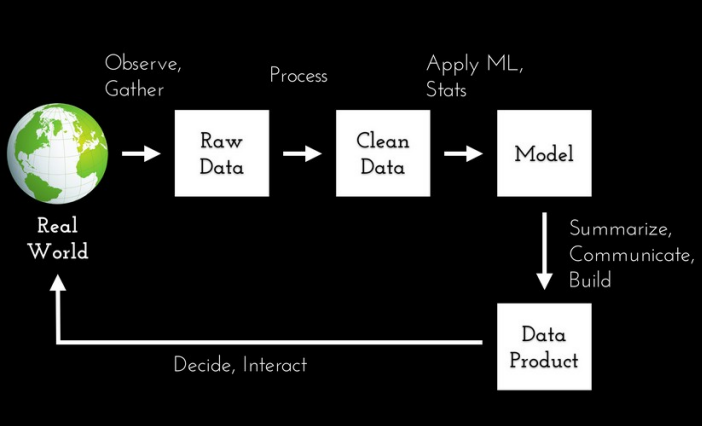
\includegraphics[width=0.5\linewidth]{images/chapter_1/Pipeline.png}
\end{figure}

In addition the Data Science Process is similar to the Knowledge Discovery in Databases (KDD).

\begin{figure}[h]
    \centering
    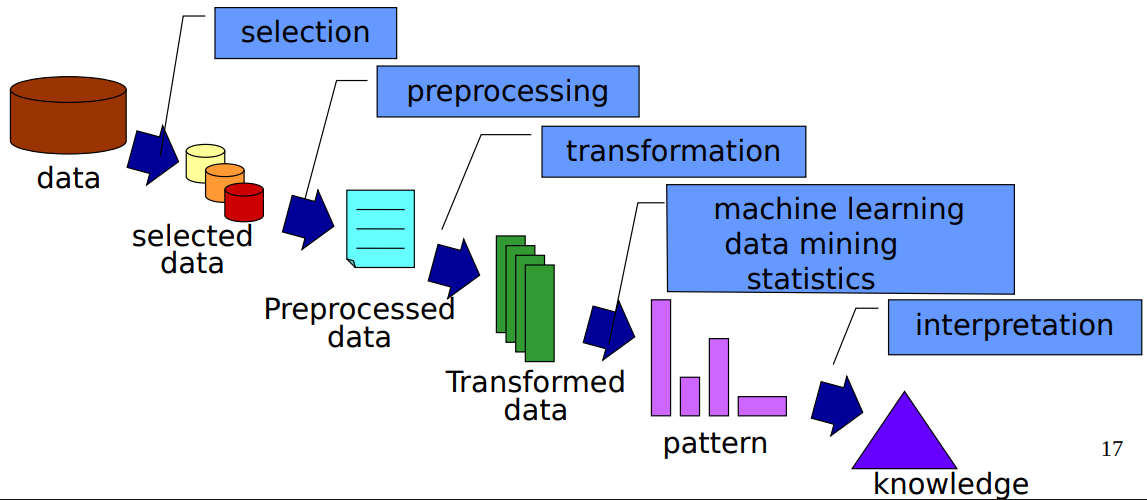
\includegraphics[width=0.5\linewidth]{images/chapter_1/Software_Pipeline.png}
\end{figure}

\subsection{Data Generation}
Data can be generated in different ways:
\begin{itemize}
    \item \textbf{Passive Recording:} log files, archives. Typically structured data.
    \item \textbf{Active Generation:} user-generated content, for instance social networks activity. Usually, semi-structured or unstructured data.
    \item \textbf{Automatic Production:} sensor-based IoT. It is location-aware, context-dependent and highly mobile data.
\end{itemize}

After the generation of data, Data Acquisition is required in order to Collect data. Transmit data to data centers and Prepocess it, in order to clean it, integrate and delete redundancies.

Data can be stored in Physical/Network Storage Infrastructures. The stored data needs then to be managed and processed by specific programming models.

\subsection{Data Preprocessing}
Real world data is considered as dirty and raw data. Without good quality data, no good quality pattern can be found. Therefore, the Data Preprocessing is needed in order to perform:
\begin{itemize}
    \item \textbf{Data Cleaning:} reducing noise effect, identifying or removing outliers and solve inconsistencies.
    \item \textbf{Data Integration:} reconciles data extracted from different sources, manages redundancy, identifies and solves data conflicts and integrates metadata.
\end{itemize}

\subsection{Data Analysis}
Data Analysis can be exploited in order to reach different objectives:
\begin{itemize}
    \item \textbf{Descriptive Analytics:} in order to know more about the data.
    \item \textbf{Predictive Analytics:} in order to take decision.
    \item \textbf{Prescriptive analytics:} in order to solve it in the future.
\end{itemize}

Different methods can be used to perform Data Analysis such as Machine Learning, data mining and statistical analysis.

It is important to note that Machine Learning and Data Mining share the common goal of extracting information from available data. Lastly, in the data science process defining the scope, techniques, evaluation of the process is advised.

\subsection{Artificial Intelligence}
ChatGPT, which is an AI language model, defines AI as the act of machines mimicking human intelligence to perform tasks. In a broader vision, the goals of AI research include reasoning, knowledge, representation, planning, learning, processing, perception, and support for robotics. To sum up, AI is the ability of a machine to imitate intelligent human behavior. Intelligence involves learning as AI Involves ML.

Therefore AI needs Machine Learning, in order to produce its intelligence.

\section{Machine Learning: Recap}

Machine Learning is all about fitting models to data in order to make predictions or forecasts.

It is important to note how Machine Learning is an application of AI. Additionally, Deep Learning is defined as an application of Machine Learning.

Inside Machine Learning, we will study the difference between Supervised and Unsupervised Learning.

\begin{figure}
    \centering
    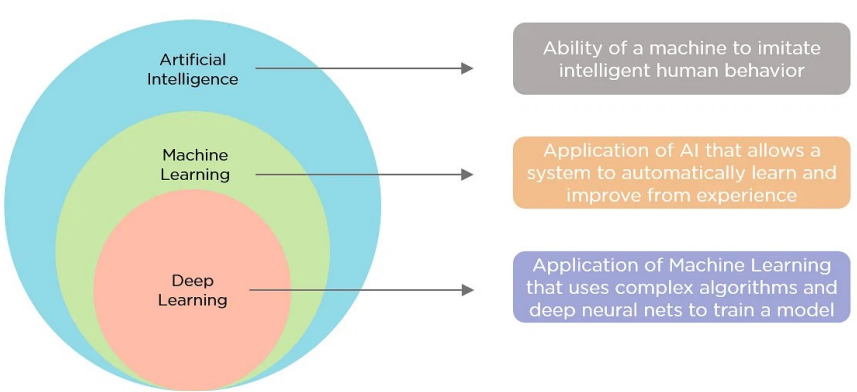
\includegraphics[width=0.5\linewidth]{images/chapter_1/ML_AI.png}
\end{figure}

To conclude, Machine Learning still faces some open issues such as the social impact derived from the interpretability and transparency of the analysis process in understandable terms to human beings. Other technical open issues are the scalability to huge data volumes, data dimensionality, data quality and the rise of heterogeneous data formats increasingly complex.


\section{A prova di coglione}
Il \textbf{Machine Learning (ML)} è un software che trova automaticamente pattern e relazioni nascosti in grandi dataset, \emph{imparando a rispondere a domande dai dati} senza che un esperto programmi ogni regola.

\paragraph*{Big Data.}
Sono dati la cui scala, diversità e complessità richiedono nuove architetture, tecniche e algoritmi per essere gestiti ed estrarne valore e conoscenza nascosta. Provengono da contenuti utente, file di log, IoT e molto altro, e si caratterizzano con le \textbf{5 V}:
\begin{itemize}
    \item \textbf{Volume}: crescita esponenziale (si è arrivati agli zettabyte);
    \item \textbf{Velocity}: generazione rapida, serve elaborazione veloce per restare tempestivi;
    \item \textbf{Variety}: formati, tipi e strutture diversi;
    \item \textbf{Veracity}: qualità a rischio (outlier, dati distorti o privi di senso), quindi accuratezza e affidabilità compromesse;
    \item \textbf{Value}: trasformare i dati in vantaggio di business, a supporto delle decisioni.
\end{itemize}

\paragraph*{Data Science.}
È la scienza che estrae significato da grandi quantità di dati, secondo un processo (simile al \textbf{KDD}) in cinque fasi: \textbf{generazione e acquisizione} (dal mondo reale ai \emph{raw data}) $\rightarrow$ \textbf{selezione} (i \emph{clean data}) $\rightarrow$ \textbf{analisi} (algoritmi e modelli statistici per trovare \emph{pattern}) $\rightarrow$ \textbf{interpretazione} (valutare, riassumere e comunicare i pattern, ottenendo il \emph{data product}) $\rightarrow$ \textbf{azione} (il data product serve a decidere o interagire con il mondo reale).

\paragraph*{Generazione e acquisizione.}
I dati nascono in tre modi: per \textbf{registrazione passiva} (log, archivi: dati strutturati), per \textbf{generazione attiva} (contenuti utente, social: semi- o non strutturati) o per \textbf{produzione automatica} (sensori IoT: dati contestuali, mobili e legati alla posizione). Segue l'\textbf{acquisizione}: raccolta, trasmissione ai data center e preprocessing (pulizia, integrazione, eliminazione delle ridondanze). I dati sono poi conservati in infrastrutture di storage fisiche o di rete e gestiti con appositi modelli di programmazione.

\paragraph*{Preprocessing.}
I dati reali sono sporchi e grezzi, e senza dati di qualità non si trovano pattern di qualità. Servono quindi:
\begin{itemize}
    \item \textbf{Cleaning}: ridurre il rumore, individuare o rimuovere gli outlier, risolvere le incoerenze;
    \item \textbf{Integration}: riconciliare dati da fonti diverse, gestire ridondanze e conflitti, integrare i metadati.
\end{itemize}

\paragraph*{Analisi dei dati.}
Persegue tre obiettivi: \textbf{descrittivo} (capire i dati), \textbf{predittivo} (prevedere per decidere) e \textbf{prescrittivo} (risolvere i problemi in futuro). Si usano ML, data mining e analisi statistica; ML e data mining condividono lo scopo di estrarre informazione dai dati. Conviene sempre definire in anticipo obiettivi, tecniche e valutazione del processo.

\paragraph*{Intelligenza Artificiale e ML.}
L'\textbf{AI} è la capacità di una macchina di imitare il comportamento intelligente umano (ragionamento, rappresentazione della conoscenza, pianificazione, apprendimento, elaborazione del linguaggio, percezione, robotica). Poiché l'intelligenza implica apprendimento, \textbf{l'AI ha bisogno del ML}. Il ML consiste nell'adattare modelli ai dati per fare previsioni; è un'applicazione dell'AI, e il \textbf{Deep Learning} è a sua volta un'applicazione del ML. Al suo interno si distingue tra apprendimento \textbf{supervisionato} e \textbf{non supervisionato}.

\paragraph*{Problemi aperti.}
L'impatto sociale, legato a \textbf{interpretabilità e trasparenza} del processo di analisi, che dovrebbe essere comprensibile all'uomo, e alcuni limiti tecnici: \textbf{scalabilità} a volumi enormi, \textbf{dimensionalità}, \textbf{qualità dei dati} e formati eterogenei sempre più complessi.
%\chapter{Data Exploration and Visualization}
A Dataset is a collection of data, for instance a tabular representation of data which includes rows (istances-records-objects) and columns (attributes). It is important to note that the rows, or the samples are in the interval $1 \rightarrow M$, while the features are from $1 \rightarrow N$. 

The size of the Dataset has an impact on the choice of the analyses:
\begin{itemize}
    \item Some algorithms require considerable HW resources when applied to large datasets.
    \item There are solutions to reduce the size of the dataset preserving the completeness of the data:
    \begin{itemize}
        \item \textbf{Data Sampling:} reduce the dataset size in terms of number or rows, records ($m' < m$).
        \item \textbf{Feature Selection:} reduce the number of attributes, features ($n' < n$).
    \end{itemize}
\end{itemize}

Features (attributes), have a major role in the Dataset. Each column of the dataset represents on attribute.Data Exploration can use a univariate approach to analyze one column in isolation, or a multivariate approach to study the relationships and dependencies between multiple columns at the same time. 

For further analysis it's useful to consider basic information for each attribute such as the unite of measurement, attribute type (categorical or numerical) and the attribute domain, by also checking if the attribute values satisfy the domain-driven constraints.

\paragraph*{Notations}
\begin{itemize}
    \item $a \in \mathcal{A}$: Object $a$ is an element of the set $\mathcal{A}$.
    \item $|\mathcal{A}|$: The cardinality (number of elements) of a finite set $\mathcal{A}$.
    \item $\mathcal{A} \subseteq \mathcal{B}$: $\mathcal{A}$ is a subset of $\mathcal{B}$.
    \item $\mathcal{A} \subset \mathcal{B}$: $\mathcal{A}$ is a strict subset of $\mathcal{B}$.
    \item $\mathbb{N}$: The set of natural numbers $1, 2, \dots$.
    \item $\mathbb{R}$: The set of real numbers.
    \item $\{0, 1\}$: The set consisting of two real-numbers 0 and 1.
    \item $[0, 1]$: The closed interval of real numbers $x$ with $0 \le x \le 1$.
    \item $\mathbf{x} = (x_1, \dots, x_n)^T$: A vector of length $n$[cite: 2].
    \item $\|\mathbf{x}\|$: The norm of the vector $\mathbf{x}$ (usually the Euclidean norm).
\end{itemize}

\section{Univariate Analysis: Distribution}
When analyzing a single feature (a column in the dataset), we can treat the general concept it measures as an abstract \textbf{Random Variable ($X$)}. The actual data points we collected ($x_1, \dots, x_m$) are the concrete samples or realizations of that variable. 

Because we can never perfectly know the underlying mathematical law that generated this data (the \textbf{theoretical distribution}), we rely entirely on our collected samples to form an \textbf{empirical distribution} (An empirical distribution is the distribution formed by data values (denoted as $x_1, \dots, x_m$) that you have collected in your dataset.), which serves as our practical, real-world approximation. The most common way to visualize this empirical distribution is through a \textbf{histogram}: we slice the total range of our data into consecutive intervals called \textbf{bins}, and simply count how many data points fall into each bin (the \textbf{frequency}).

Probability Distributions are usually classified as:
\begin{itemize}
    \item \textbf{Discrete Probability Distribution:} discrete list of probabilities of outcomes and described by a probability mass function.
    \begin{figure}[h]
        \centering
        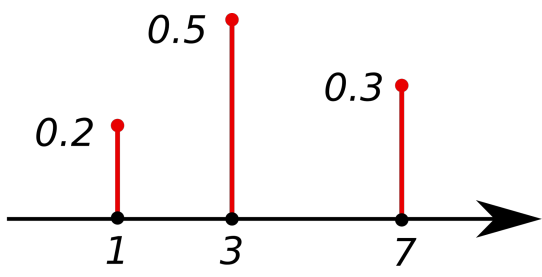
\includegraphics[width=0.3\linewidth]{images/chapter_2/PMF.png}
        \caption{Example of a Probability Mass Function (PMF)}
    \end{figure}
    
    \item \textbf{Continuous Probability Distribution:} set of possible outcomes can assume values in a continuous range and described by a probability density function.
    \begin{figure}[h]
        \centering
        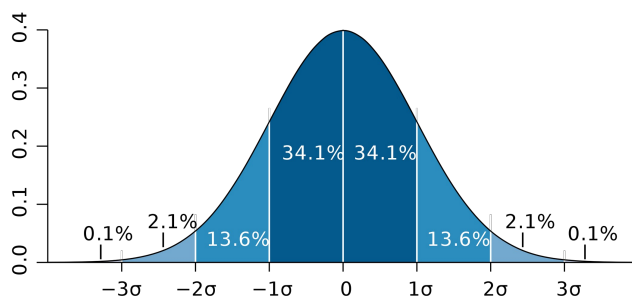
\includegraphics[width=0.3\linewidth]{images/chapter_2/PDF.png}
        \caption{Example of the Probability Density Function (PDF) of the normal distribution}
    \end{figure}
\end{itemize}

\subsection{Discrete and Continuous Probability Recall}
The Probability Mass Function present some limitations:

\begin{itemize}
    \item In cases of a lot of samples to show it is very hard to read information from a PFM plot. Possible solutions include calculating the Cumulative Distribution Function (CDF) and showing the difference of distribution.
\end{itemize}

While for Continuous Probability an example of the PDF is a Gaussian Distribution.  

\subsection{KDE: Kernel Density Estimation}
Kernel Density Estimation (KDE) estimates the continuous probability density function based on collected samples. It can be viewed as a smoother, continuous version of the histogram that more closely approximates the real Probability Density Function (PDF). The main features of KDE are:

\begin{itemize}
    \item It estimates the function $f$ as a weighted average of neighboring observed data points.
    \item The weight is defined by a \textbf{Kernel function ($K$)}, which ensures that data points closer to the evaluation point receive higher weights.
    \item The resulting estimated function is continuous and smooth.
\end{itemize}

The general formula for the KDE of a function, given $m$ samples $x_i$, is defined as:
$$\hat{f}_h(x) = \frac{1}{mh} \sum_{i=1}^m K\left(\frac{x-x_i}{h}\right)$$

\begin{figure}[h]
    \centering
    \includegraphics[width=0.5\linewidth]{images/chapter_2/KDE Example.png}
    \caption{KDE Example}
\end{figure}

This formula relies on two critical components:
\begin{itemize}
    \item \textbf{The Kernel ($K$):} A common choice is the standard Gaussian distribution, defined as $K(z) = \frac{1}{\sqrt{2\pi}} e^{-z^2 / 2}$.
    \item \textbf{The Bandwidth ($h$):} This parameter determines the width of the kernel (e.g., the spread of the Gaussian bell) and controls the level of smoothness. Misspecifying the bandwidth $h$ can heavily distort the representation of the data: an \textbf{over-smoothed} curve can erase true features of the underlying distribution, while an \textbf{under-smoothed} curve can create false features generated by random noise.
\end{itemize}

\begin{figure}[h]
    \centering
    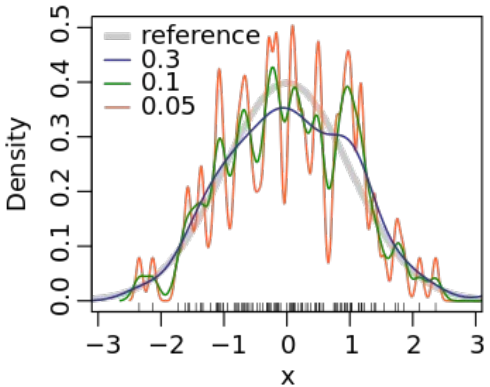
\includegraphics[width=0.4\linewidth]{images/chapter_2/Bandwidth.png}
    \caption{KDE Bandwidth}
\end{figure}

To summarize, compared to a histogram, KDE produces plots that are much less cluttered and highly interpretable. However, it suffers from potential distortions if the underlying distribution has hard boundaries or lacks smoothness, and its accuracy heavily depends on selecting the appropriate smoothing parameter (bandwidth).

\subsection{CDF: Cumulative Distribution Function}
The Cumulative Distribution Function (CDF) is a function of $x$, where $x$ represents any value that might appear within a given distribution. 

Probability that a random variable $X$ will take a value less than or equal to a specific value $x$, :
$$F_X(x) := P(X \le x)$$

Also used to calculate the probability that a value falls within a specific interval between $a$ and $b$:
$$P(a \le X \le b) = F_X(b) - F_X(a)$$

The CDF provides a clear visual representation of the distribution's overall shape. Highly probable values and common intervals appear as steep, nearly vertical sections on the CDF graph, indicating a high concentration of data points in that specific range. Conversely, flat sections indicate ranges with very few data points.

\begin{figure}[h]
    \centering
    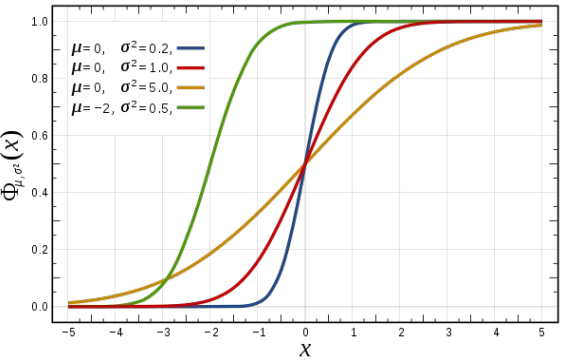
\includegraphics[width=0.4\linewidth]{images/chapter_2/CDF_Example.png}
    \caption{CDF}
\end{figure}

\subsection{ECDF: Empirical Cumulative Distribution Function}
The Empirical Cumulative Distribution Function (ECDF) is an estimate of the CDF that generated the points in the sample. To evaluate ECDF($x$) for a particulare value of $x$, it is needed to compute the fraction of values in the distribution less than or equal to $x$. ECDF is a step function that jumps up by $1/m$ at each of the $m$ data points. It's a really good estimation of the CDF, even if it's a step function.

\subsection{Percentiles}
Percentile indicates the value below which a given percentage of observations in a group of observation falls. Representing a feature through percentiles allow representing its entire distribution. The most famous percentiles are the quartiles $25^{th}$, $50^{th}$, and $75^{th}$.It is useful to remember than the $50^{th}$ represents the median, as 50\% of the values are smaller than it and the remaining 50\% are bigger. It is the mean only for the Gaussian Distribution. Finally, the outliers are easily found as for example they can be the values in the first and last percentile of the distribution.

\begin{figure}[h]
    \centering
    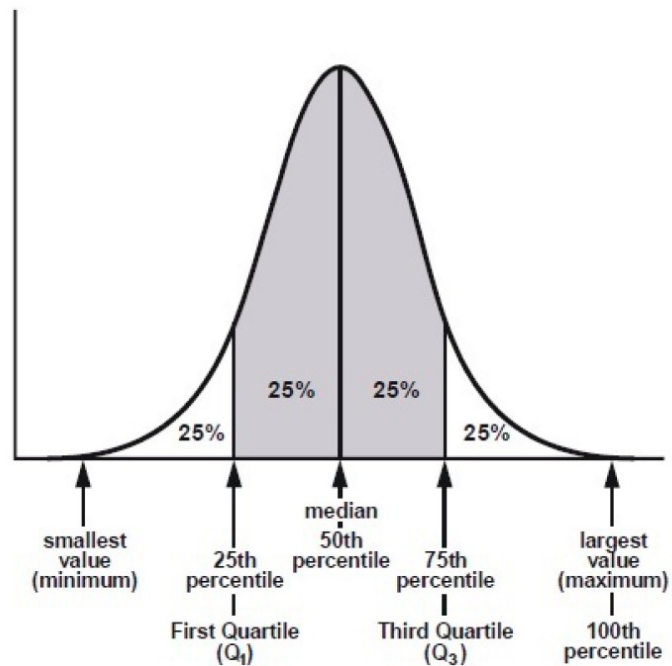
\includegraphics[width=0.5\linewidth]{images/chapter_2/Percentile.png}
\end{figure}

\subsection{Boxplot}
Boxplots are a standardized way of displaying the distribution of data based on summary values:


\begin{itemize}
    \item \textbf{Median:} $50^{th}$ percentile ($Q2$) the middle value of the attribute, not the mean.
    \item \textbf{First Quartile:} middle number between the smallest number excluding outliers (not minimum) and the median of the attribute.
    \item \textbf{Third Quartile:} the middle value between the median and the highest value excluding outliers (not the maximum) of the attribute.
    \item \textbf{Interquatile Range (IQR):} $25^{th}$ to the $75^{th}$ percentile.
    \item \textbf{Whiskers:} lines that exit from the boxplot (shown in blue).
    \item \textbf{Outliers:} samples (points) that fall outside of the range: $(Q1 - (1.5 * IQR)) \rightarrow (Q3 + (1.5 * IQR))$
\end{itemize}

\begin{figure}[h]
    \centering
    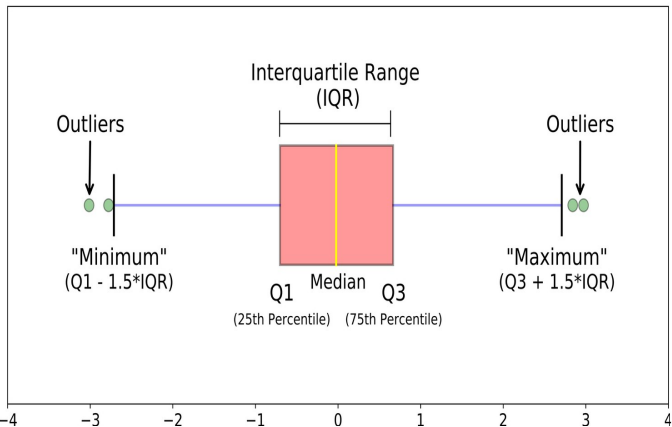
\includegraphics[width=0.4\linewidth]{images/chapter_2/Boxplot.png}
\end{figure}

It is important to know that box plot won't be symmetrical if the underlying distribution is not a Gaussian distribution.

\begin{figure}[h]
    \centering
    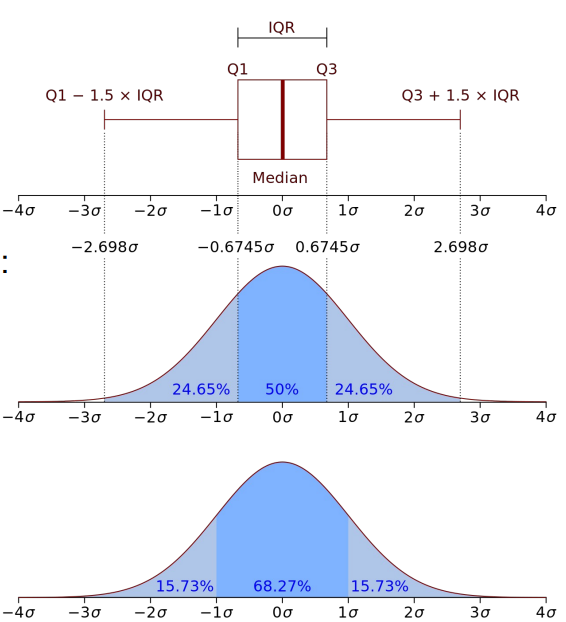
\includegraphics[width=0.4\linewidth]{images/chapter_2/Boxplot Example.png}
\end{figure}

\subsection{Outliers}
Outliers are extreme values that might be errors in measurement and recording or rather accurate reports of rare events. The best way to define and handle outliers depends on domain knowledge, such as information about where the data come from, what they mean and the scope of the analysis.Outliers can be detected through univariate analysis (boxplots, percentiles, GESD) or multivariate analysis (DBSCAN).

\begin{itemize}
    \item \textbf{GESD:} Generalized Extreme Studentized Deviate is used to detect one or more outliers in a univariate dataset that follows a normal distirbution. The GESD test performs separate tests for 1 outlier up to an upper bound $k$ of outliers, where a test statistic $R$ is recomputed recursively up to the $k$-th outlier.
    \item \textbf{DBSCAN:} is density based clustering non parametric algorithm used in multivariate analysis, as it groups together points that are closely packed together (points with many nearby neighbors), while marking as outliers points that lie alone in low density regions, whose nearest neighbors are too far away.
\end{itemize}

\begin{figure}[h]
    \centering
    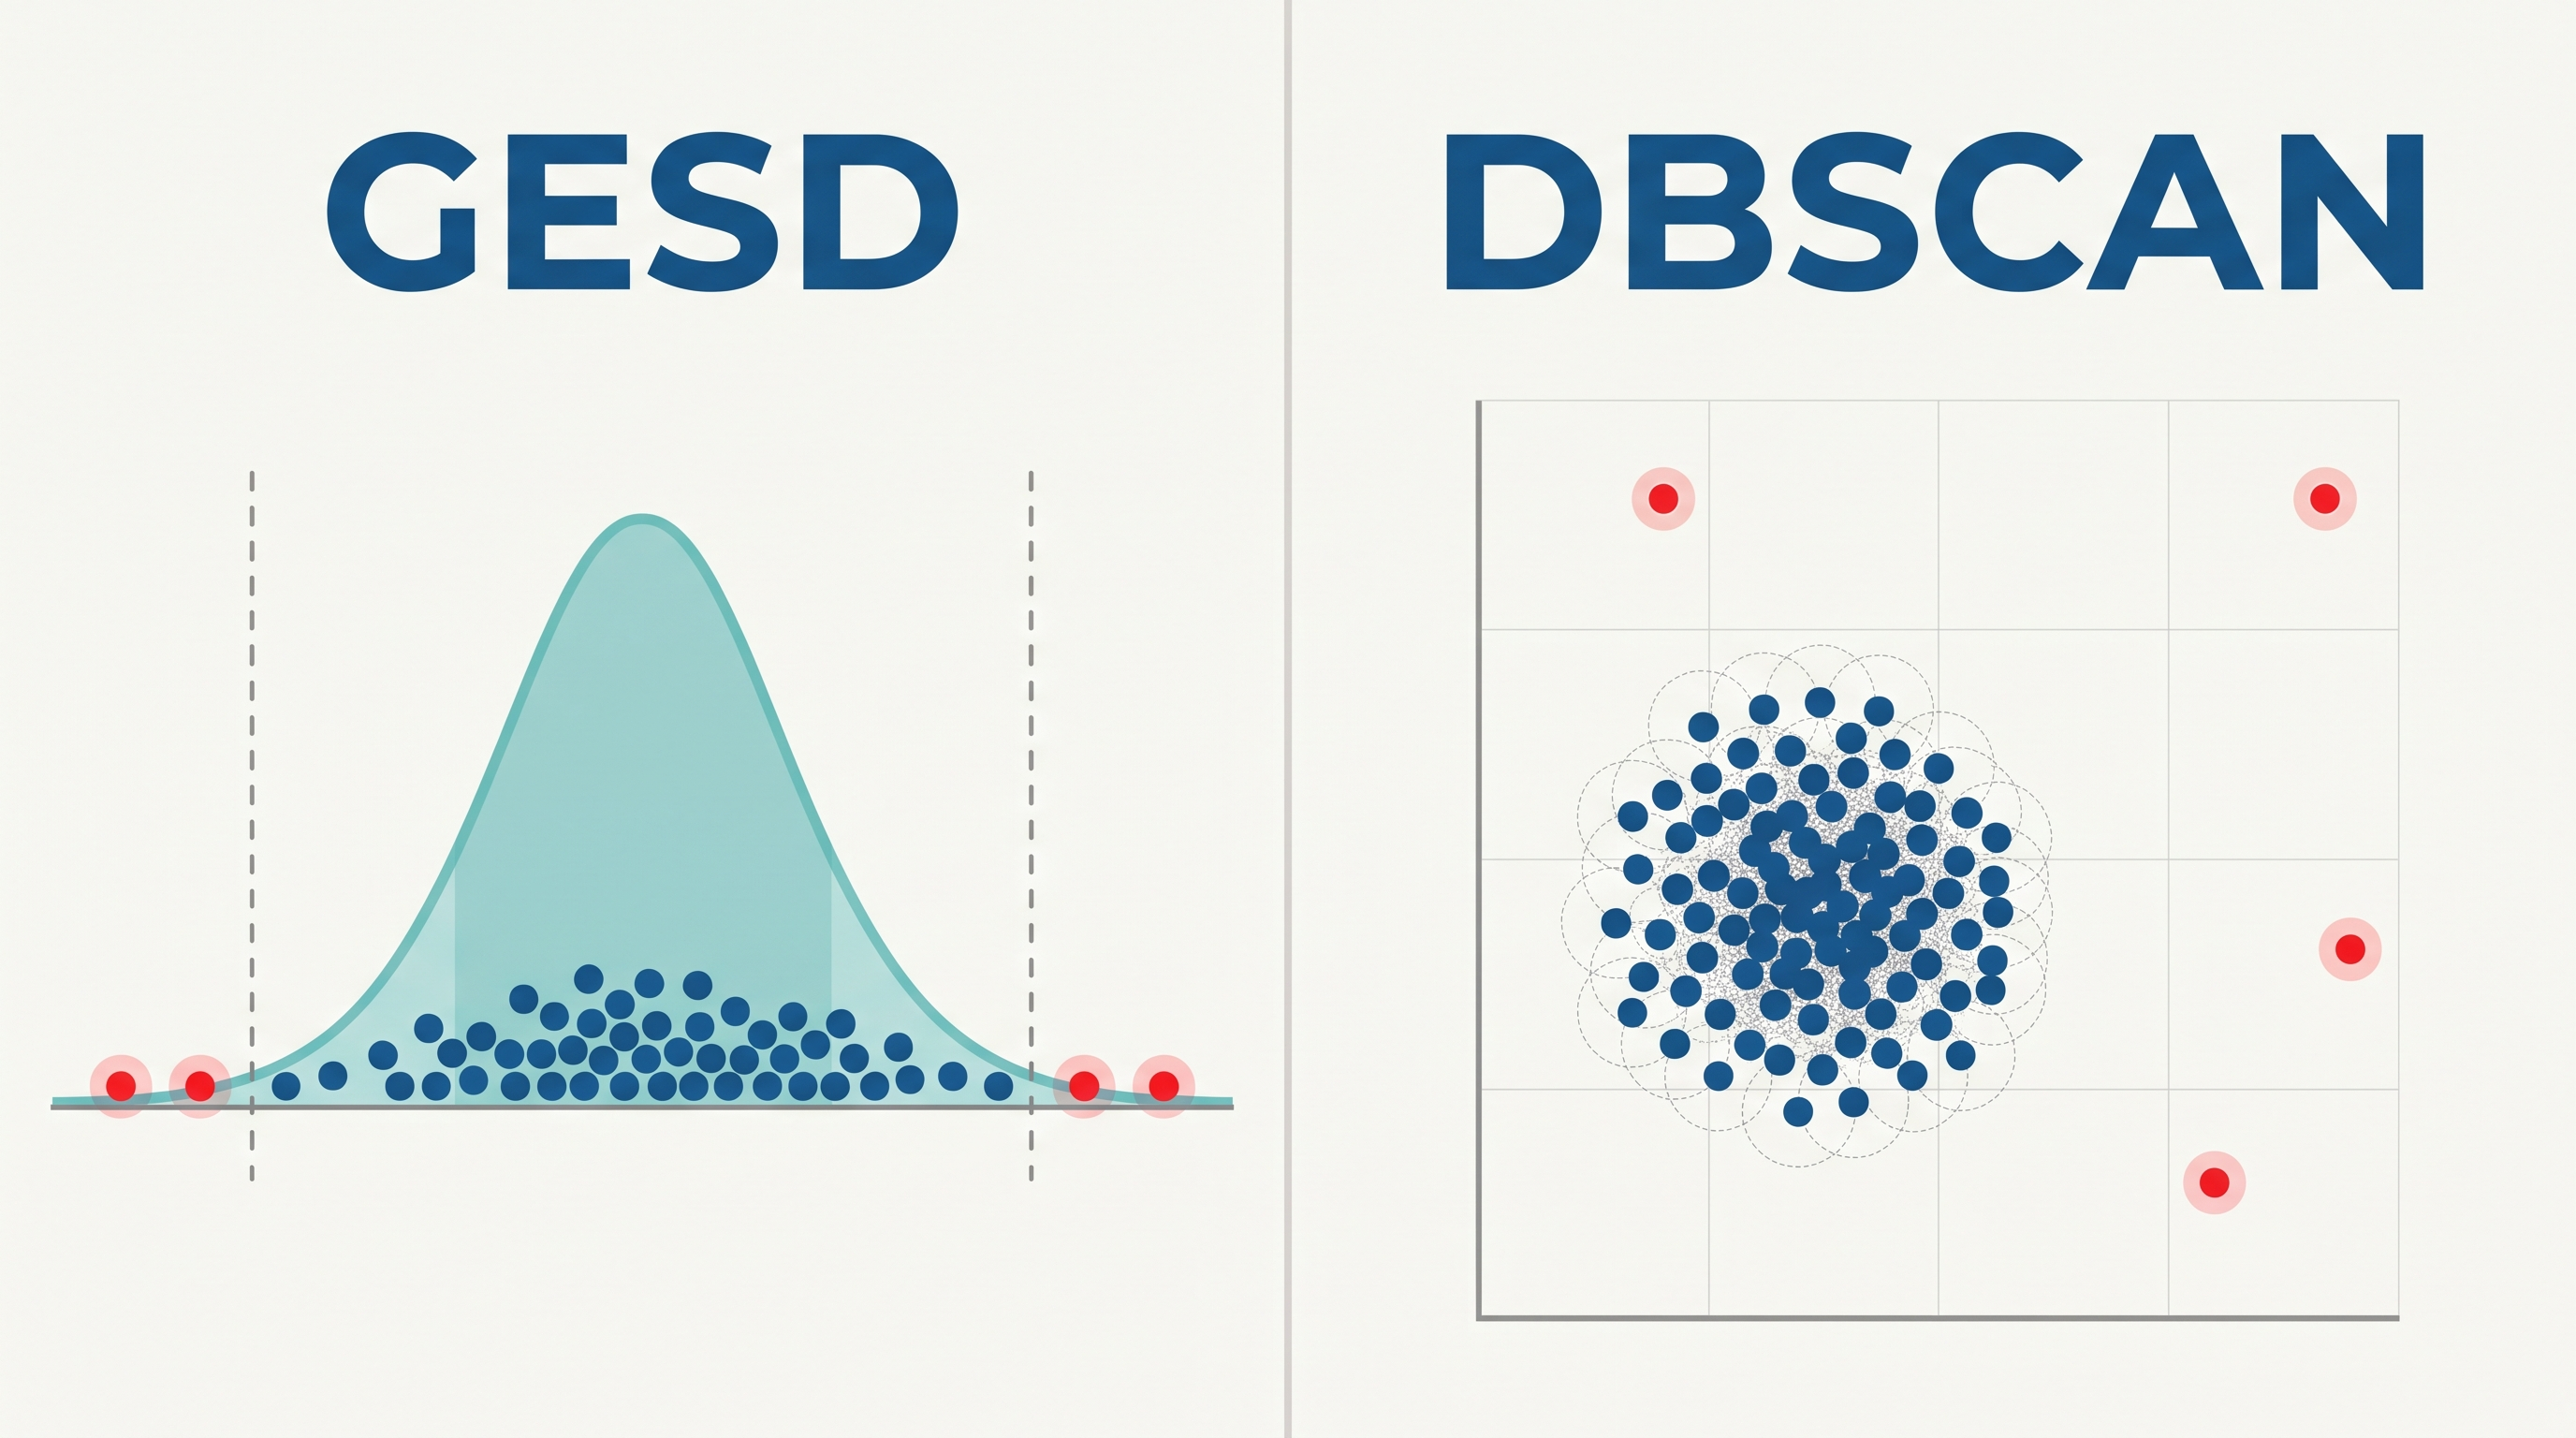
\includegraphics[width=0.4\linewidth]{images/chapter_2/GESD_DBSCAN.png}
\end{figure}

\section{Correlation Analysis}
Datasets usually include different features and the description of the main relations, namely the correlation, between different features assumes a key role.The correlation is the measure of the relationship between two data objects and it is useful during the data exploration phase in order to perform analysis of feature correlation.

\subsection{Scatter Plot}
Scatter plots are the simplest way to visually check for a relationship between 2 variables, but they don't allow you to see if there are many points in the same position or just one, since the data are affected by rounding and conversion. A possible solution to this issue is to jitter the data by adding noise to reverse the effect of rounding off. 

\begin{figure}[h]
    \centering
    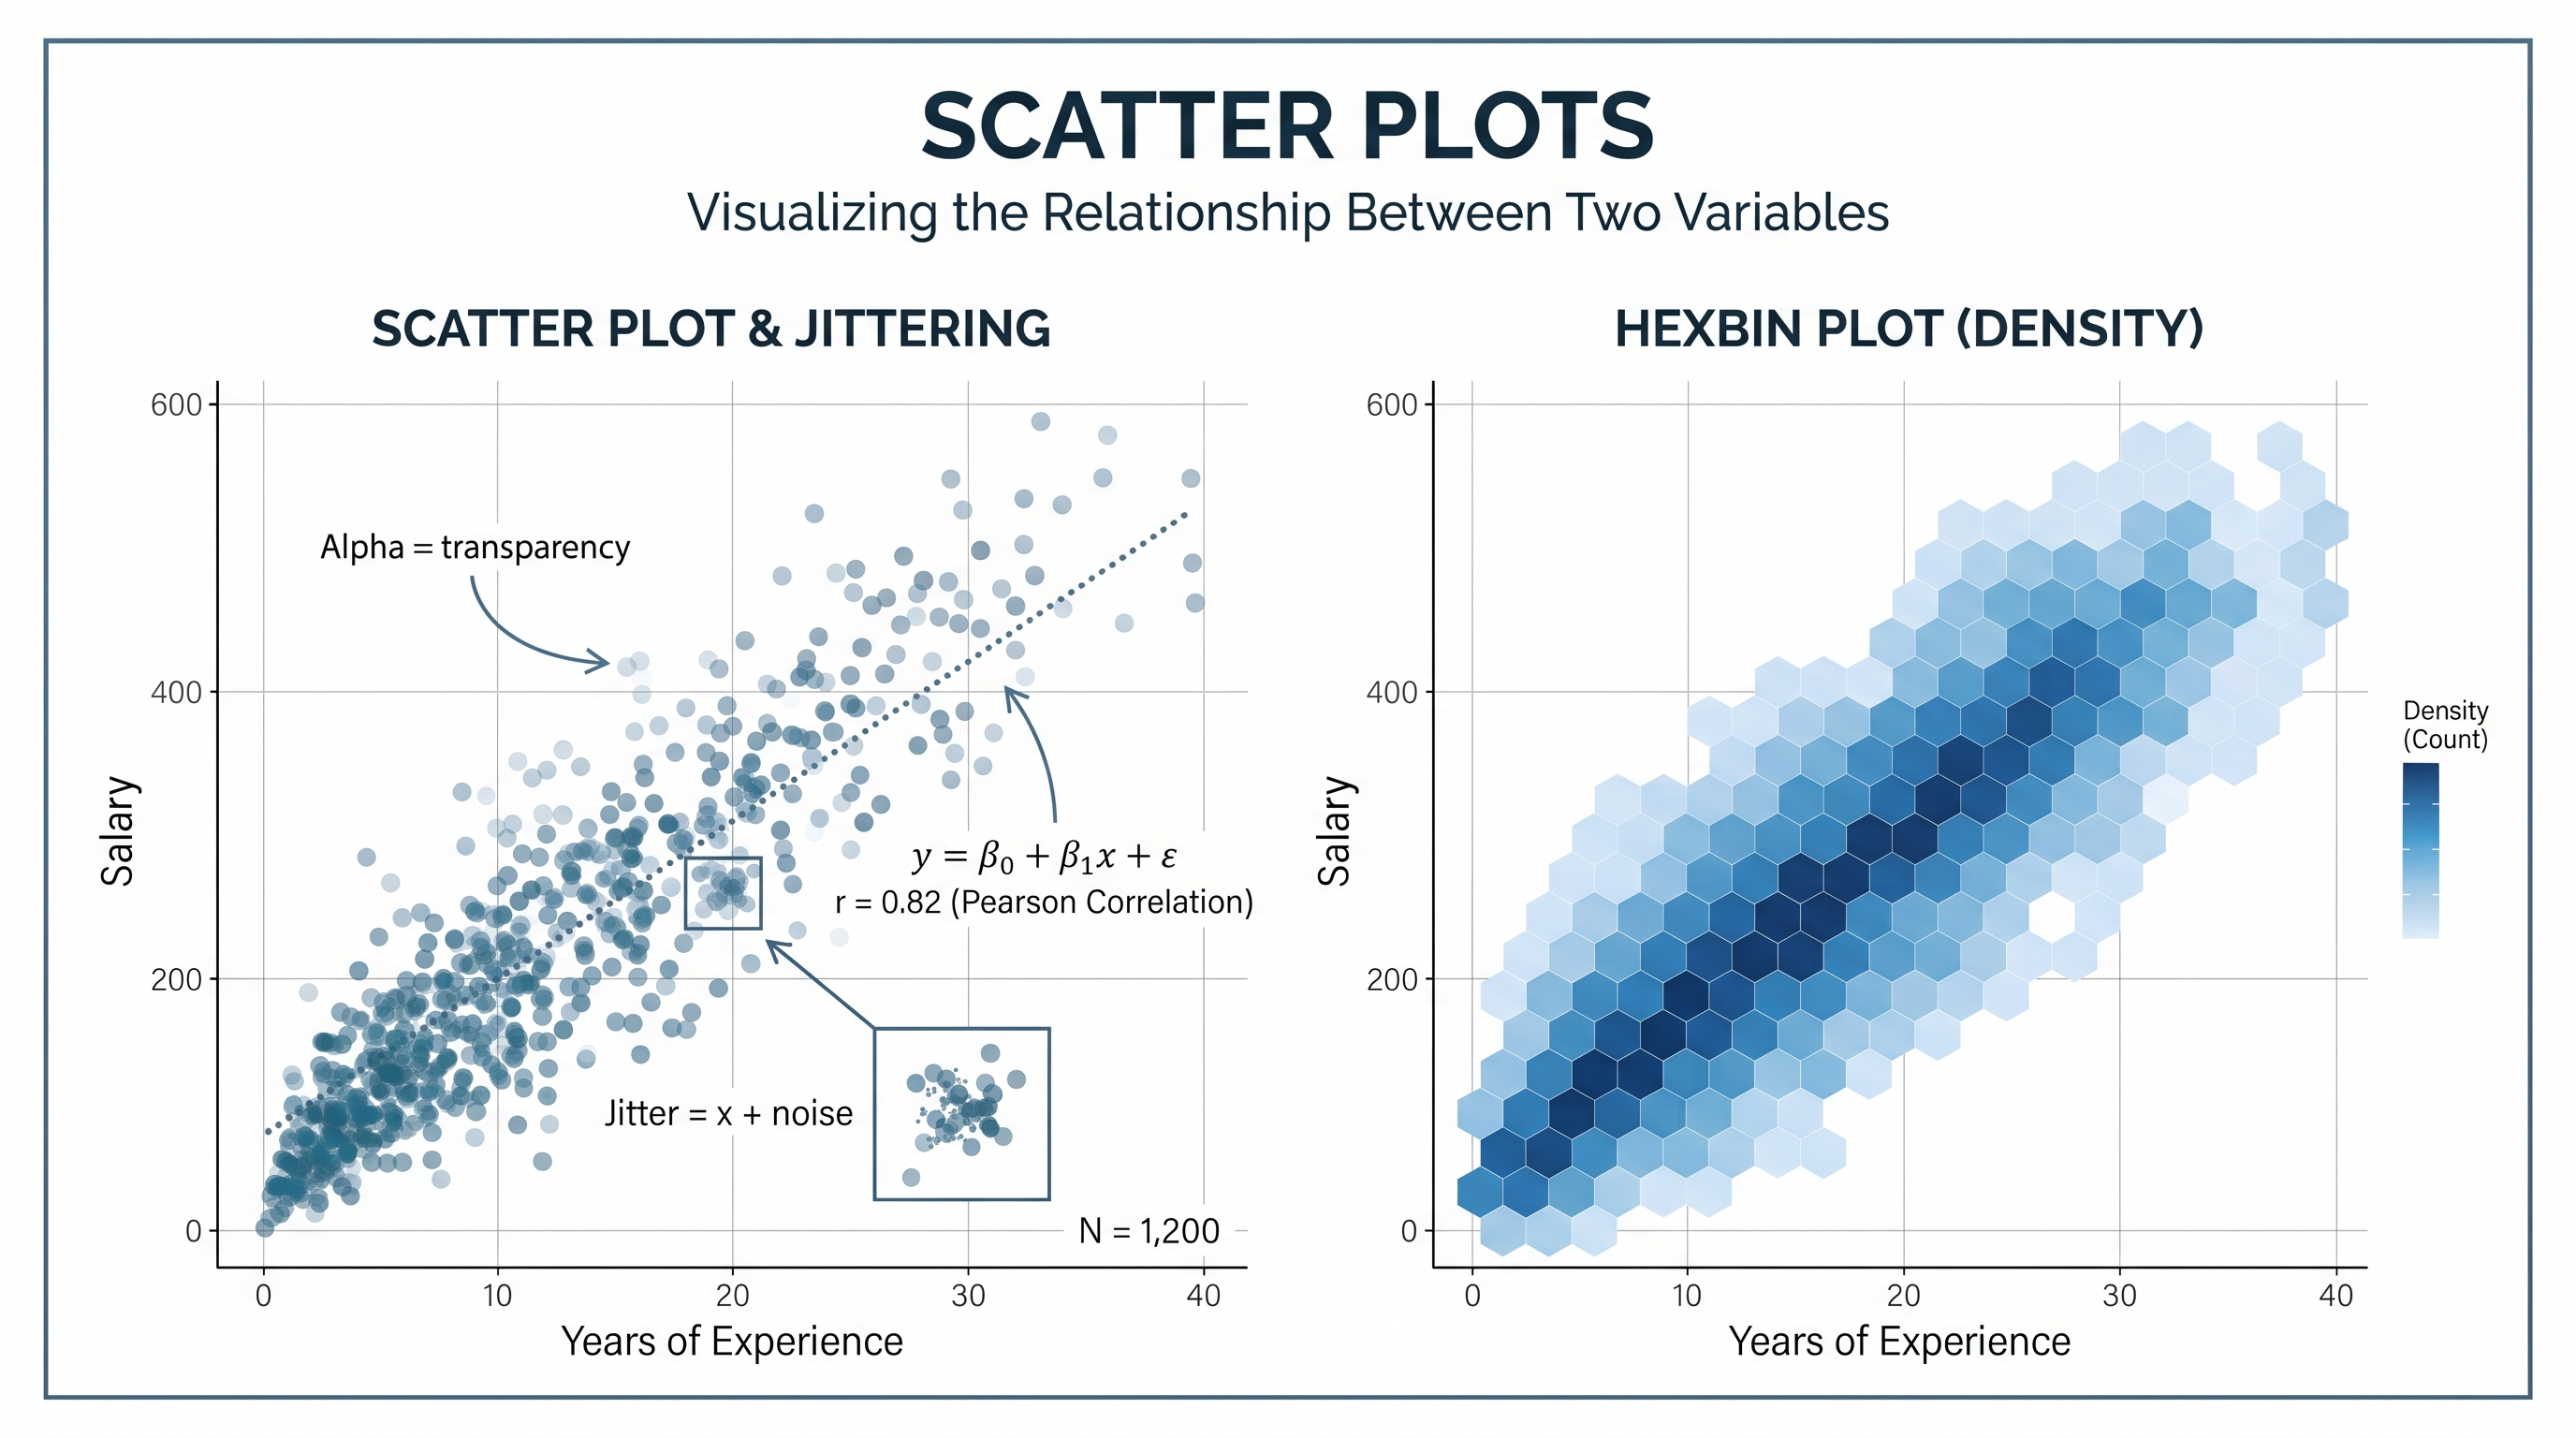
\includegraphics[width=0.35\linewidth]{images/chapter_2/Scatter.png}
    \caption{Scatter Plot}
\end{figure}

Then adding an alpha parameter (transparency) to each point in order to retrieve density information, where darker zones correspond to higher density zones. There is also the possibility to build hexbin plots and scatter plot percentiles, where it is required to bin one variable and plot a curve for the two variables in each bin.Moreover, Correlation is a statistic quantity indented to quantify the strength of the relationship between 2 variables. There are different ways to compute correlations:

\begin{itemize}
    \item \textbf{Covariance:} in order to compare two variables they must have same unit of measurement or alternatively be normalised.
    \item \textbf{Pearson's Correlation} is a single number that states how much 2 features are meanly correlated, if -1 negatively correlated, if 1 perfectly positively correlated. 0 for not linear correlated. Pearson's Correlation solves the problem of normalization, needed by the Covariance, but it only detects linear correlation, so for instance it is unable to detect quadratic correlation, and all the other non-linear correlations.
\end{itemize}

\begin{figure}[h]
    \centering
    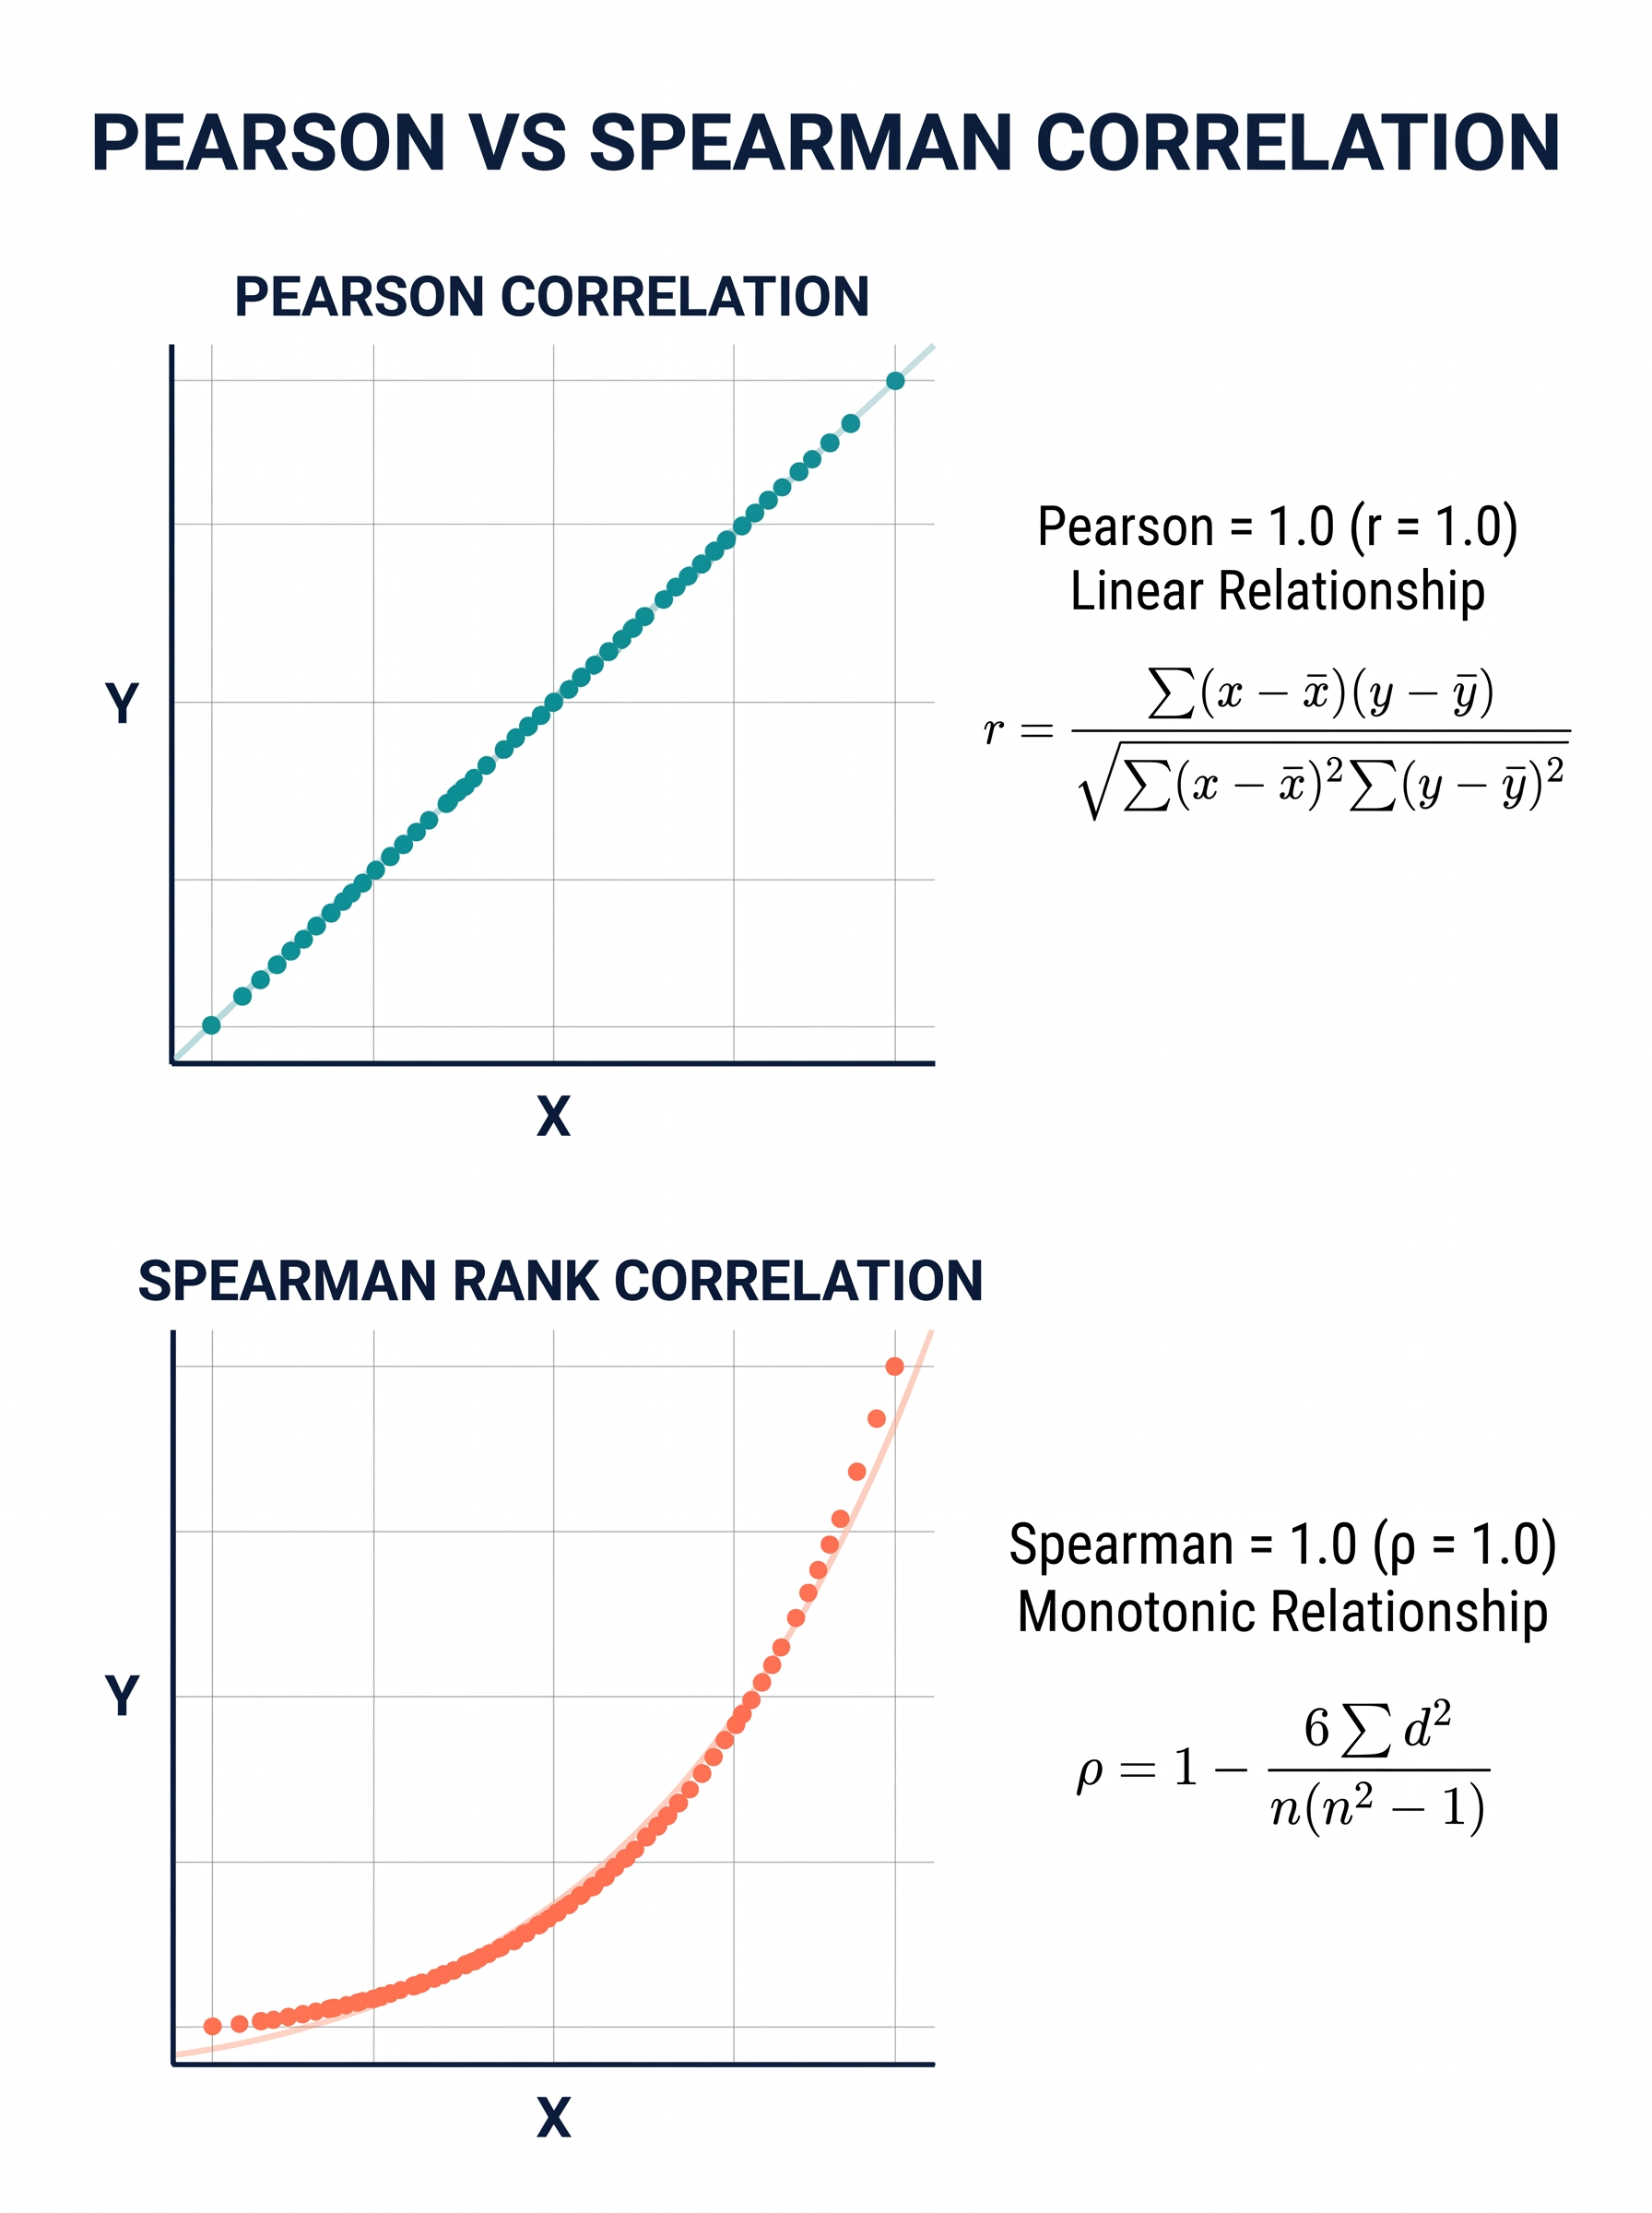
\includegraphics[width=0.35\linewidth]{images/chapter_2/Pearson_Spearman.png}
    \caption{Pearson and Spearman Correlation}
\end{figure}

\begin{figure}[h]
    \centering
    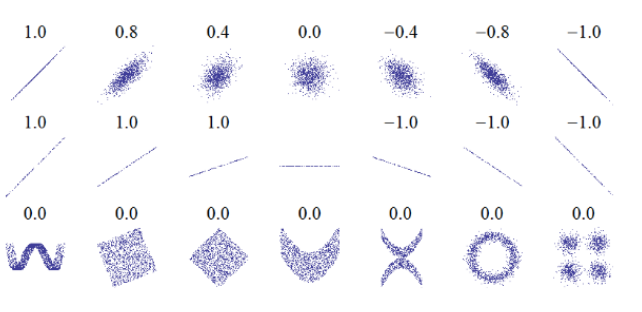
\includegraphics[width=0.35\linewidth]{images/chapter_2/Pearson_non_Linear_correlation.png}
    \caption{Pearson Non Linear Correlation}
\end{figure}

In addition, there are some types of nonlinear correlations that Pearson's correlation can't detect, such as perfectly horizontal, if one variable is always constant the formula doesn't detect it.

\begin{itemize}
    \item \textbf{Spearman's Rank Correlation:} Spearman index uses the variables rank instead of Pearson that used the variables themselves. It assesses how well the relationship between 2 variables can be described using a monotonic function. In some cases the Spearman index saves from some corner cases of Pearson index returning a value close to 0. The method for applying it is the following:
    \begin{itemize}
        \item Rank the 2 dataset, ranking is achieved by giving the ranking 1 to the biggest number in a column, 2 to the second biggest one and so on. The smallest value in the column will get the lowest ranking.
        \item If using the simplified rank formula: Indicate $m$ as the number of different ranks.
        \item Tied scores are given the mean (average) rank. For example, if there are 3 tied scores ranked $5^{th}$ ($5^{th}$, $6^{th}$, $7^{th}$) the mean rank is calculated as $(5+6+7)/3 = 6$.
        \item Find the difference in the ranks, that is the difference between the ranks of the two values on each row.
        \item Compute the formula, either in the general case or in the integer simplified case.
    \end{itemize}
\end{itemize}

\textbf{Spearman's Rank Correlation Example:} $X = (3,0,1)$, $Y = (-1,50,2)$
\begin{enumerate}
    \item rank both datasets: $X=(1,3,2)$ $Y=(3,1,2)$
    \item indicate $m$ as the number of different ranks, in this case $m = 3$
    \item compute the difference $X_i - Y_i$: $(-2,2,0)$
    \item use the formula, in this case the simplified integer ranks formula: $r_s = 1 - (6 * (4 + 4))/(3 - 8) = -1$
\end{enumerate}

\begin{figure}[h]
    \centering
    \includegraphics[width=0.35\linewidth]{images/chapter_2/chapter_2/Spearman_Rank_Examples.png}
\end{figure}

In addition Spearman's rank is 1 when both variable are correlated by an increasing monotonic function, while -1 if the function is decreasing monotonic. 0 if there isn't a monotonic function correlation. To sum up, Spearman's rank detects monotonic correlation between 2 variables, not only linear correlation as Pearson does.

\section{Data Visualization: Advanced Techniques}

\subsection{Heatmap}
A heatmap is a colorful grid that makes it easy to read a correlation matrix. Instead of looking at raw numbers to see how strongly two variables are linked, you look at colors. For example, a dark red square might mean a strong positive relationship, while a dark blue one means a strong negative relationship. The grid is perfectly symmetric: the relationship between variable A and variable B is the exact same as the relationship between B and A.

\begin{figure}[h]
    \centering
    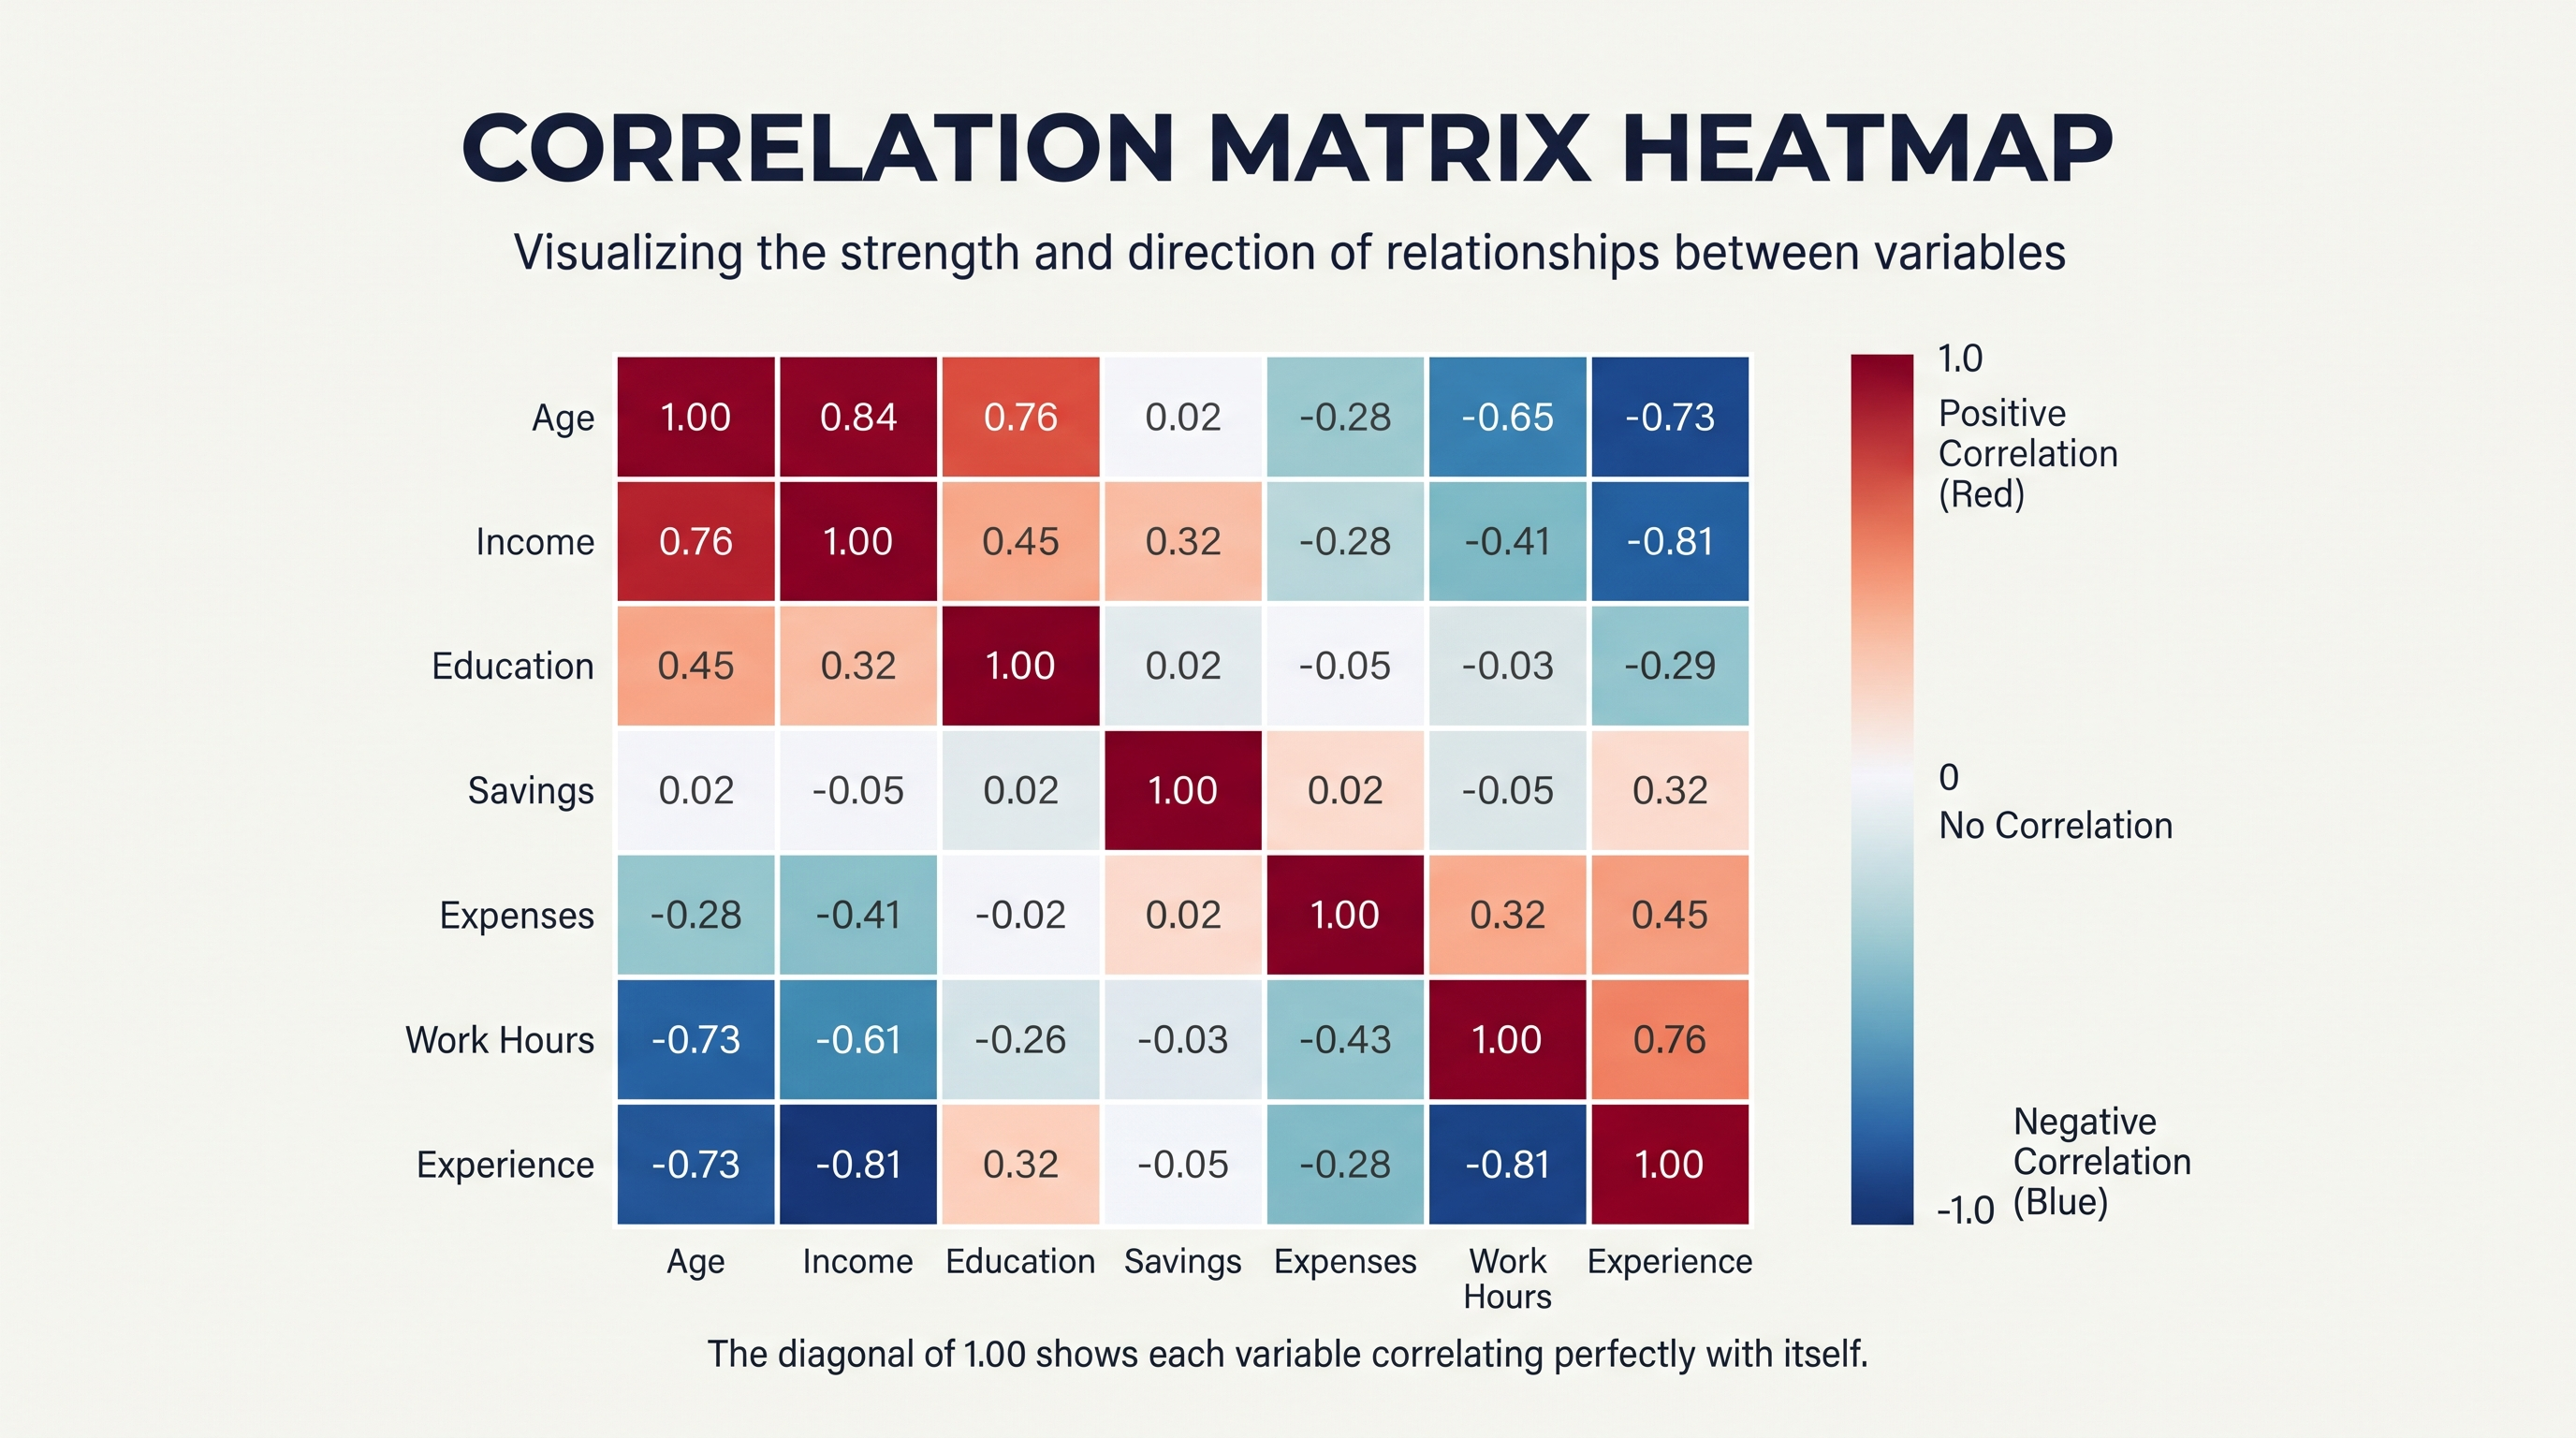
\includegraphics[width=0.5\linewidth]{images/chapter_2/Heatmap.png}
\end{figure}

\subsection{Dimensionality Reduction: PCA and t-SNE}
When a dataset has dozens or hundreds of features, plotting it on a standard 2D graph is impossible. To fix this, we use mathematical techniques to compress the dataset into just 2 or 3 new features without losing too much important information. 

\begin{figure}[h]
    \centering
    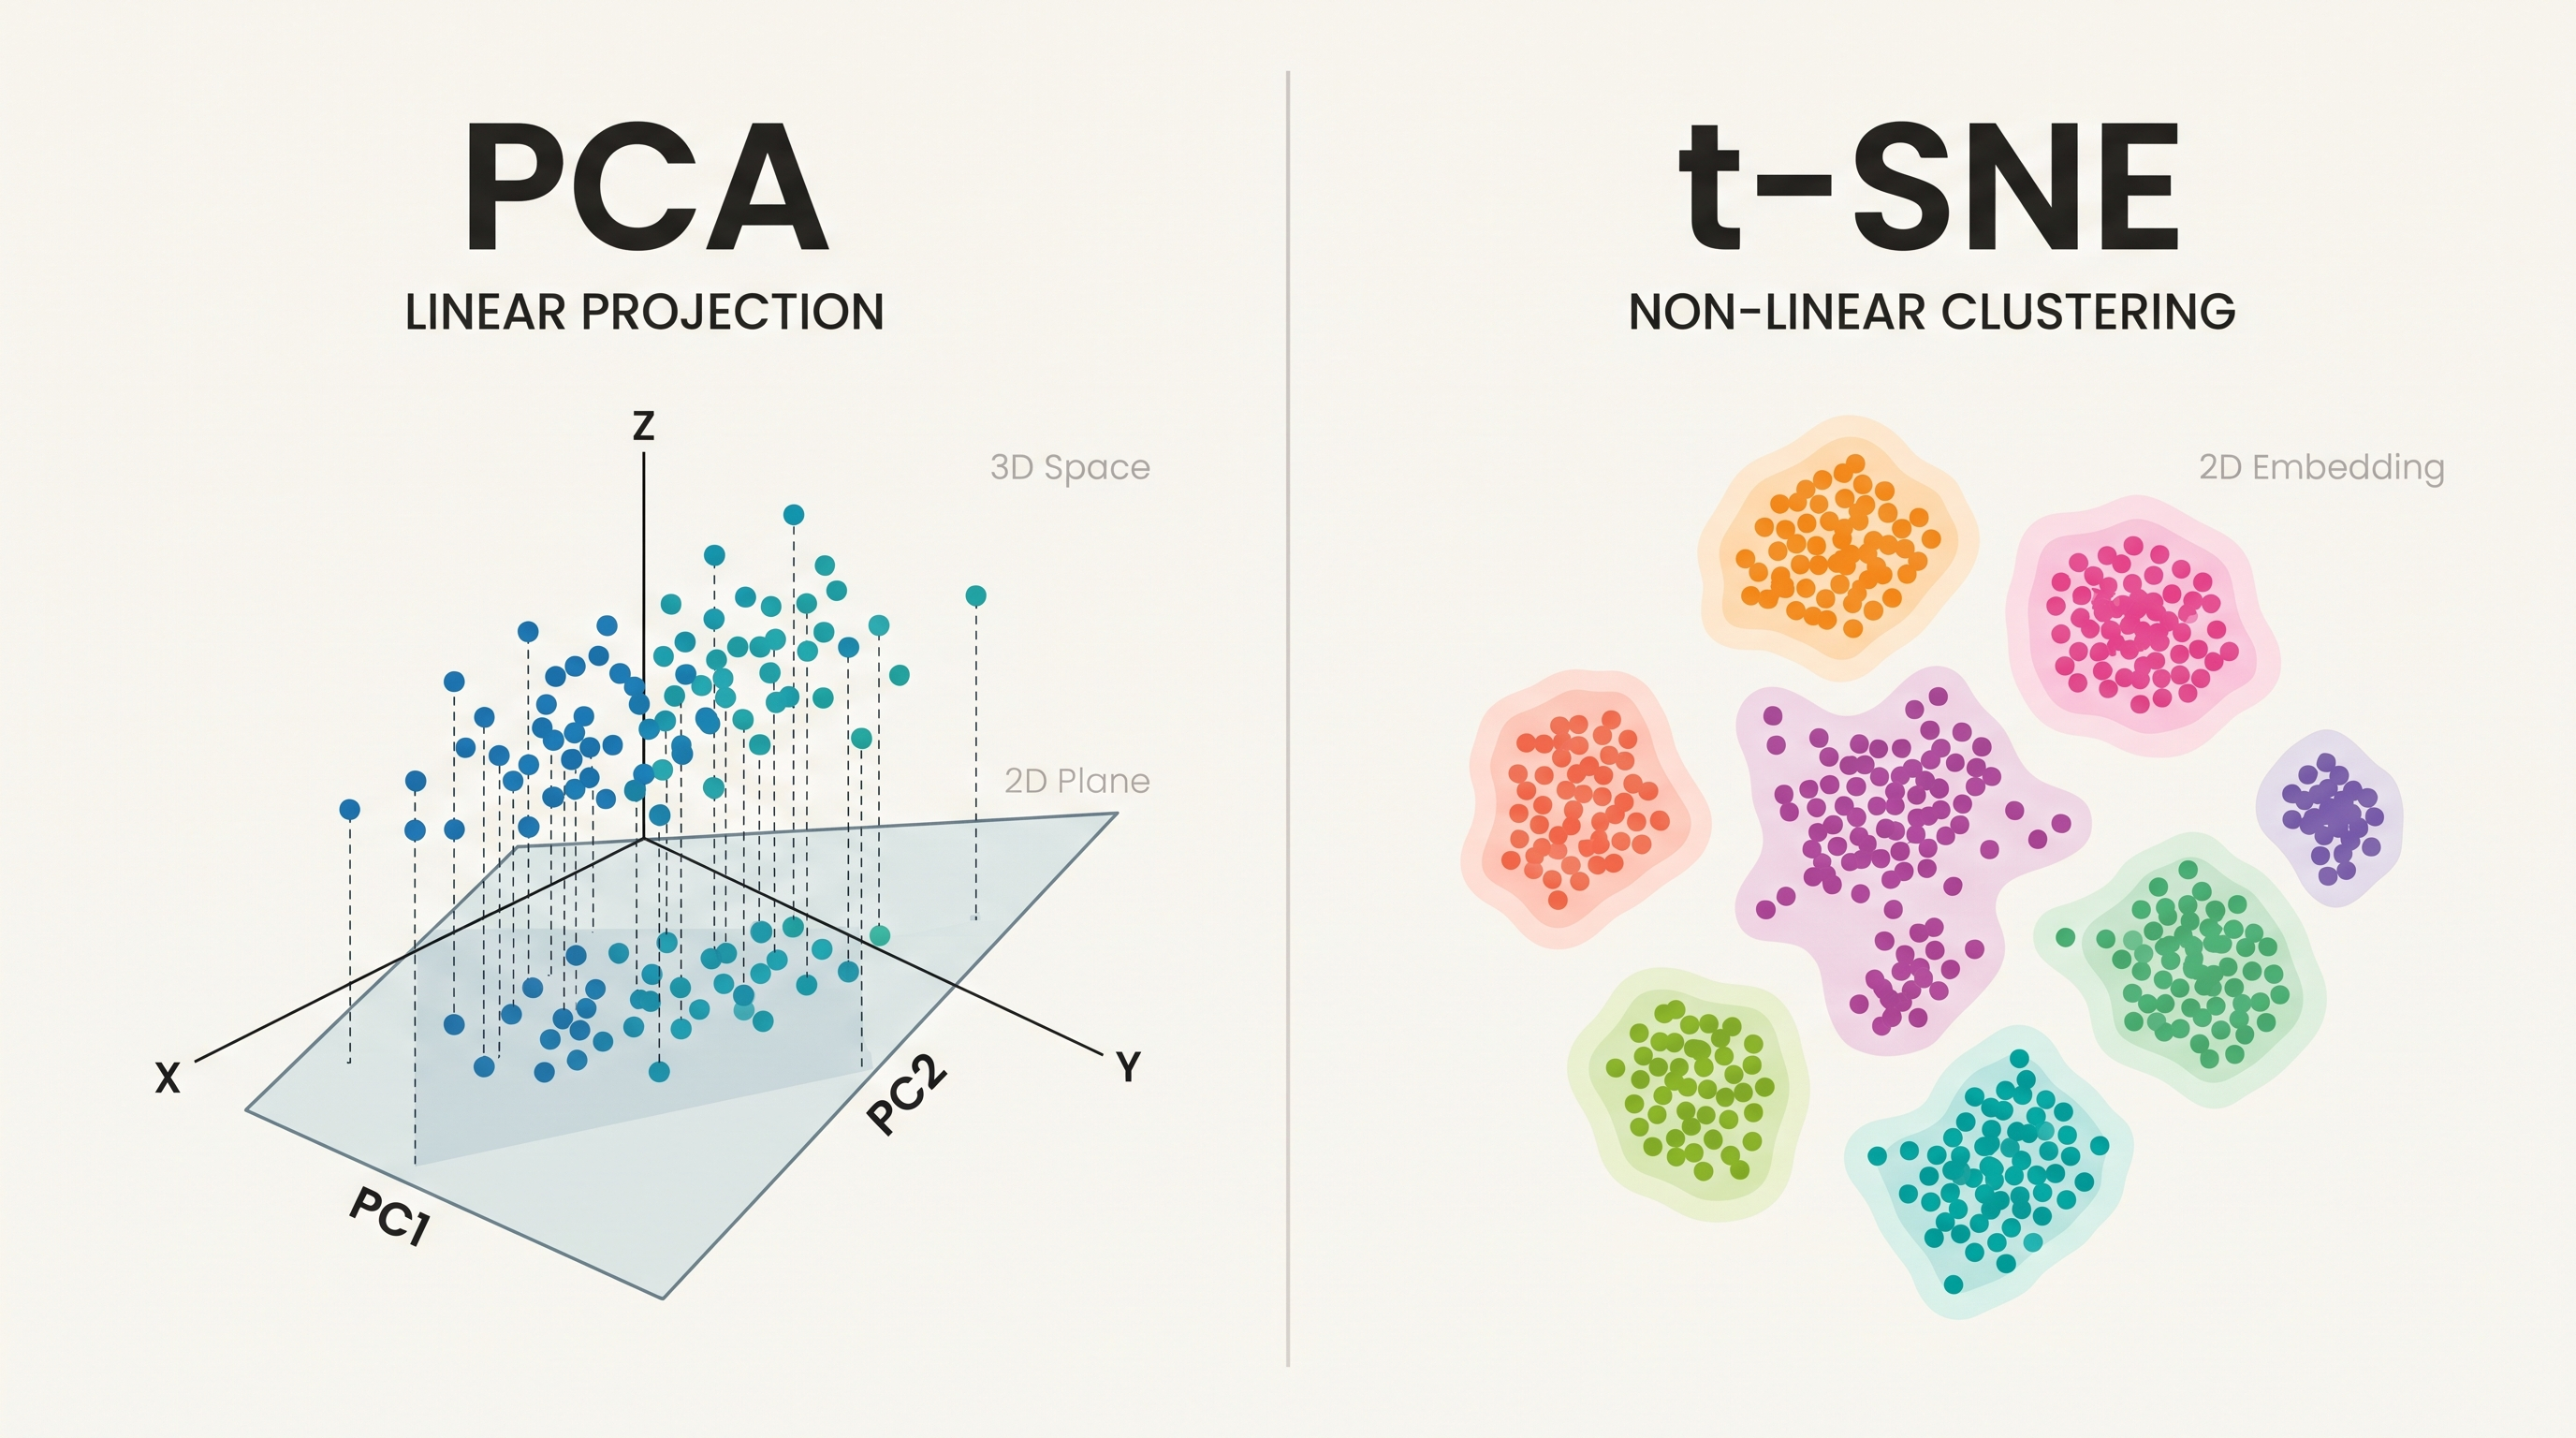
\includegraphics[width=0.5\linewidth]{images/chapter_2/PCA_tSNE.png}
\end{figure}

\begin{itemize}
    \item \textbf{PCA (Principal Component Analysis):} This method shrinks the data by finding the main linear directions that contain the most information. It provides a broad, global overview of the dataset's general trends.
    \item \textbf{t-SNE (t-Distributed Stochastic Neighbor Embedding):} This is a more complex, non-linear technique. It focuses on keeping similar data points close to each other, making it excellent for spotting distinct groups or clusters on a 2D map.
\end{itemize}

Visualizing data is crucial for understanding it, but picking the right chart or reduction method depends entirely on what underlying patterns you want to discover.


\section{A prova di coglione}

\paragraph*{Il dataset.}
Tabella di $M$ righe (istanze, record, oggetti, campioni) e $N$ colonne (attributi, feature). Le sue dimensioni condizionano l'analisi, perché alcuni algoritmi richiedono molte risorse hardware su dataset grandi. Si riducono con il \textbf{data sampling} (meno righe, $m'<m$) o con la \textbf{feature selection} (meno colonne, $n'<n$). L'esplorazione può essere \textbf{univariata} (una colonna alla volta) o \textbf{multivariata} (relazioni tra più colonne). Per ogni attributo servono unità di misura, tipo (categorico o numerico) e dominio, verificando che i valori rispettino i vincoli del dominio. Notazione usata: $a\in\mathcal A$ (appartenenza), $|\mathcal A|$ (cardinalità), $\subseteq$ e $\subset$ (sottoinsieme e sottoinsieme stretto), $\mathbb N$, $\mathbb R$, $\{0,1\}$, $[0,1]$, vettore $\mathbf x=(x_1,\dots,x_n)^T$ e norma $\|\mathbf x\|$ (di solito euclidea).

\subsection*{Analisi univariata: la distribuzione}

Una feature è una \textbf{variabile aleatoria} $X$ e i dati raccolti $x_1,\dots,x_m$ sono le sue realizzazioni. La legge che li ha generati (\textbf{distribuzione teorica}) è ignota, quindi ci si affida alla \textbf{distribuzione empirica}, di solito visualizzata con un \textbf{istogramma}: l'intervallo dei dati è diviso in \emph{bin} consecutivi e se ne conta la frequenza. Le distribuzioni sono \textbf{discrete} (descritte da una funzione di massa, PMF) o \textbf{continue} (descritte da una funzione di densità, PDF, come la gaussiana). Con molti campioni la PMF è illeggibile: si ricorre alla CDF o al confronto tra distribuzioni.

\paragraph*{KDE (Kernel Density Estimation).}
Stima la PDF dai campioni ed è una versione \emph{liscia e continua} dell'istogramma. Calcola la densità come media pesata dei punti vicini, con pesi dati da un \textbf{kernel} $K$ (tipicamente gaussiano) più alti per i punti più prossimi:
$$\hat f_h(x)=\frac{1}{mh}\sum_{i=1}^m K\!\left(\frac{x-x_i}{h}\right)$$
La \textbf{bandwidth} $h$ controlla la levigatezza. Se è troppo grande (\emph{over-smoothing}) cancella caratteristiche reali, se è troppo piccola (\emph{under-smoothing}) crea caratteristiche false dovute al rumore. Rispetto all'istogramma il grafico è più pulito e leggibile, ma si distorce con distribuzioni dai bordi netti o non lisce e dipende dalla scelta di $h$.

\paragraph*{CDF ed ECDF.}
La \textbf{CDF} $F_X(x)=P(X\le x)$ dà la probabilità di restare sotto $x$, e $P(a\le X\le b)=F_X(b)-F_X(a)$. I tratti ripidi indicano valori frequenti, quelli piatti zone quasi vuote. L'\textbf{ECDF} la stima dai campioni: è la frazione di valori $\le x$, una funzione a gradini che sale di $1/m$ a ogni dato, ma approssima molto bene la CDF.

\paragraph*{Percentili e boxplot.}
Il \textbf{percentile} è il valore sotto cui cade una data percentuale delle osservazioni, quindi i percentili descrivono l'intera distribuzione. I più usati sono i quartili (25°, 50°, 75°); il 50° è la \textbf{mediana}, che coincide con la media solo nella gaussiana. Il \textbf{boxplot} riassume la distribuzione con: mediana ($Q2$), $Q1$ e $Q3$ (calcolati escludendo gli outlier), \textbf{IQR} (da $Q1$ a $Q3$), \emph{whiskers} (i baffi) e \textbf{outlier}, i punti fuori da $[\,Q1-1.5\,\mathrm{IQR},\;Q3+1.5\,\mathrm{IQR}\,]$. Se la distribuzione non è gaussiana, il boxplot non è simmetrico.

\paragraph*{Outlier.}
Valori estremi che possono essere errori di misura o registrazione, oppure segnalazioni corrette di eventi rari: come trattarli dipende dalla conoscenza del dominio (origine dei dati, significato, scopo dell'analisi). Si rilevano con metodi univariati (boxplot, percentili, GESD) o multivariati (DBSCAN):
\begin{itemize}
    \item \textbf{GESD}: test per trovare uno o più outlier in un dataset univariato \emph{normale}; ripete i test da 1 fino a un massimo di $k$ outlier, ricalcolando la statistica $R$.
    \item \textbf{DBSCAN}: clustering non parametrico basato sulla densità; raggruppa i punti molto vicini e segna come outlier quelli isolati in zone a bassa densità, con vicini troppo lontani.
\end{itemize}

\subsection*{Analisi di correlazione}

La \textbf{correlazione} misura la relazione tra due variabili e guida l'esplorazione delle feature.

\paragraph*{Scatter plot.}
È il modo più semplice per vedere una relazione tra due variabili, ma arrotondamenti e conversioni sovrappongono i punti, nascondendone la densità. Si rimedia con il \textbf{jitter} (rumore che annulla l'effetto dell'arrotondamento), con la \textbf{trasparenza} $\alpha$ (zone scure = alta densità), con gli \textbf{hexbin} o con gli \textbf{scatter plot a percentili} (una variabile divisa in bin, con una curva per ciascun bin).

\paragraph*{Indici di correlazione.}
\begin{itemize}
    \item \textbf{Covarianza}: confronta due variabili solo se hanno la stessa unità di misura o sono normalizzate.
    \item \textbf{Pearson}: un solo numero che risolve la normalizzazione, $-1$ per correlazione negativa perfetta, $+1$ per positiva perfetta, $0$ per assenza di correlazione \emph{lineare}. Vede solo relazioni lineari: non coglie quelle quadratiche o non lineari in genere, né il caso di una variabile costante.
    \item \textbf{Spearman}: usa i \emph{ranghi} invece dei valori e misura quanto la relazione sia descrivibile da una funzione \textbf{monotona}. Vale $1$ se la funzione è crescente, $-1$ se decrescente, $0$ se non c'è monotonia. Evita alcuni casi limite in cui Pearson dà valori vicini a 0.
\end{itemize}

\textbf{Calcolo di Spearman.} Si assegnano i ranghi a ogni colonna (1 al valore maggiore, e così via; i pari merito ricevono il rango medio, ad esempio tre valori al 5°, 6°, 7° posto ricevono $(5+6+7)/3=6$), si calcolano le differenze $d_i$ tra i ranghi di ogni riga e si applica, per ranghi interi e $m$ ranghi distinti,
$$r_s=1-\frac{6\sum_i d_i^2}{m(m^2-1)}$$
\emph{Esempio}: $X=(3,0,1)$ e $Y=(-1,50,2)$ hanno ranghi $(1,3,2)$ e $(3,1,2)$, quindi $d=(-2,2,0)$ e $r_s=1-\frac{6\cdot 8}{3\cdot 8}=-1$ (relazione monotona decrescente).

\subsection*{Visualizzazione avanzata}

\begin{itemize}
    \item \textbf{Heatmap}: griglia colorata che rende leggibile una matrice di correlazione al posto dei numeri (rosso scuro = correlazione positiva forte, blu scuro = negativa forte). È simmetrica, perché la relazione A–B coincide con quella B–A.
    \item \textbf{Riduzione di dimensionalità}: con decine o centinaia di feature non si può tracciare un grafico 2D, quindi si comprime il dataset in 2 o 3 nuove feature perdendo poca informazione. \textbf{PCA} trova le direzioni lineari principali che contengono più informazione e dà una visione globale delle tendenze. \textbf{t-SNE} è non lineare e mantiene vicini i punti simili, ottimo per individuare gruppi e cluster.
\end{itemize}

Visualizzare è fondamentale per capire i dati, ma il grafico o la riduzione giusti dipendono dai pattern che si vogliono scoprire.
%\chapter{Data PreProcessing}

\section{Data Types and Properties}
Attribute values are assigned to an attribute for a particular object. It is useful to remember the difference between attributes and attribute values, as the same attribute can be mapped to different attribute values (for instance, height can be measured in feet or meters). Moreover, different attributes can be mapped to the same set of values (for example, both ID and age can be integers).

There are 2 main attribute types:
\begin{itemize}
    \item \textbf{Categorical (Nominal):} for instance ID numbers, eye color.
    \item \textbf{Ordinal:} for instance time, count, grades. A set of ordered attribute values.
\end{itemize}

The main difference between these 2 attribute types resides in the properties of the corresponding attribute values:
\begin{itemize}
    \item \textbf{Nominal (Categorical) Attribute Property:} Distinctness, operator ($=$).
    \item \textbf{Ordinal Attribute Properties:} Distinctness and Order, operators ($<$, $=$, $>$).
\end{itemize}

Moreover, there are Discrete and Continuous Attributes:
\begin{itemize}
    \item \textbf{Discrete Attribute:} finite set of values, often represented as integer variables. Binary attributes are a special case of discrete attributes.
    \item \textbf{Continuous Attribute:} real numbers as attribute values. In practice, real values can only be measured and represented using a finite number of digits.
\end{itemize}

Regarding Data Types we have:
\begin{itemize}
    \item \textbf{Tabular Data:} collection of records, each of them characterized by a fixed set of attributes.
    \item \textbf{Document Data:} semi-structured or unstructured textual data.
    \item \textbf{Graph Data:} for instance the World Wide Web.
    \item \textbf{Ordered Data:} for instance spatio-temporal data or genomic sequences.
\end{itemize}

\begin{table}[h]
    \centering
    \begin{tabular}{@{}lll@{}}
        \toprule
        \textbf{Tipo di attributo} & \textbf{Proprietà / operatori} & \textbf{Esempi} \\
        \midrule
        Nominale (categorico) & Distinzione ($=$) & ID, colore degli occhi \\
        Ordinale & Distinzione e ordine ($<$, $=$, $>$) & Voti, taglie S/M/L \\
        \midrule
        Discreto & Insieme finito, spesso interi & Conteggi, binari (0/1) \\
        Continuo & Numeri reali (cifre finite) & Altezza, temperatura \\
        \midrule
        \multicolumn{3}{@{}l}{\textbf{Tipi di dati}} \\
        Tabellari & Record con attributi fissi & Dataset clienti \\
        Documenti & Testo semi/non strutturato & Articoli, email \\
        Grafi & Nodi e collegamenti & World Wide Web \\
        Ordinati & Sequenze spazio-temporali & Genoma, serie storiche \\
        \bottomrule
    \end{tabular}
    \caption{Riepilogo di attributi e tipi di dati}
\end{table}

\subsection{Data Quality}
Each dataset comes with data quality issues, represented by:
\begin{itemize}
    \item \textbf{Noise and Outliers:} Noise refers to the modification of original values, for instance noise can be introduced in the data recording process. It is important to note that noise is considered to be randomly distributed. On the other hand, outliers are data objects with characteristics that are considerably different from most of the other data in the dataset. Outliers can be noise that interferes with the data analysis, or they can also be the goal of the data analysis.
    \item \textbf{Missing Values:} either the information is not collected or some attributes may not be applicable to all cases. Missing values must be handled by eliminating them, estimating them or ignoring them during the analysis.
    \item \textbf{Duplicate Data:} the dataset may include data objects that are duplicates, or almost duplicates, of one another. It is a major issue when merging data from heterogeneous sources, and Data Cleaning is needed.
\end{itemize}

\section{Similarity and Dissimilarity in Data}
\textbf{Similarity} is the numerical measure of how alike two data objects are. It is a metric that often falls in the $[0,1]$ range and is higher when objects are more alike. \textbf{Dissimilarity} is the numerical measure of how different 2 data objects are. It is lower when objects are more alike and is often a \textbf{distance metric}.

\subsection{Similarity and Dissimilarity for Simple Attributes}
A \textbf{dissimilarity} $d(x,y)$ is a numerical measure of how \emph{different} two data objects are: it is $0$ when the objects are identical and grows as they become more different. A \textbf{similarity} $s(x,y)$ measures how \emph{alike} two objects are: it is usually bounded in $[0,1]$, with $1$ meaning identical. The two notions are complementary, so similarity is typically obtained by transforming dissimilarity.
 
For simple attributes (1 dimension), the appropriate measure depends on the attribute type, since each type supports different operations:
 
\begin{center}
    \small
    \renewcommand{\arraystretch}{1.4}
    \begin{tabular}{|l|p{4.6cm}|p{5.2cm}|}
    \hline
    \textbf{Attribute Type} & \textbf{Dissimilarity} & \textbf{Similarity} \\
    \hline
    Nominal & $d=0$ if $x=y$; \newline $d=1$ if $x\neq y$ & $s=1$ if $x=y$; \newline $s=0$ if $x\neq y$ \\
    \hline
    Ordinal & $d=\dfrac{|x-y|}{n-1}$ \newline (values mapped to integers $0$ to $n-1$, where $n$ is the number of values) & $s=1-d$ \\
    \hline
    Interval or Ratio & $d=|x-y|$ & $s=-d$, \quad $s=\dfrac{1}{1+d}$, \quad $s=e^{-d}$, \newline $s=1-\dfrac{d-\min d}{\max d-\min d}$ \\
    \hline
    \end{tabular}
\end{center}
 
\paragraph{Nominal attributes.} Only the equality operator is meaningful, so two values are either identical or different: there is no notion of ``more different''. For example, $d(\text{red},\text{red})=0$, while $d(\text{red},\text{blue})=d(\text{red},\text{green})=1$.
 
\paragraph{Ordinal attributes.} Values have an order, so some pairs are farther apart than others. The values are first mapped to consecutive integers $0,\dots,n-1$, and the difference is divided by $n-1$ so that $d\in[0,1]$. For example, with $\{\text{poor},\text{fair},\text{good},\text{excellent}\}$ we have $n=4$ and the mapping $\{0,1,2,3\}$:
\[
d(\text{poor},\text{good})=\frac{|0-2|}{3}=\frac{2}{3}, \qquad s=1-\frac{2}{3}=\frac{1}{3}.
\]
Note that this approach implicitly assumes that consecutive values are equally spaced, which is not always true.
 
\paragraph{Interval and ratio attributes.} The natural dissimilarity is the absolute difference $d=|x-y|$, which ranges in $[0,+\infty)$. Different transformations turn it into a similarity, all decreasing as $d$ increases:
\begin{itemize}
    \item $s=-d$: simplest choice, but not bounded in $[0,1]$;
    \item $s=\frac{1}{1+d}$: ranges in $(0,1]$, with $s=1$ when $d=0$;
    \item $s=e^{-d}$: ranges in $(0,1]$ and decreases faster;
    \item $s=1-\frac{d-\min d}{\max d-\min d}$: min-max normalization over the dataset, ranges in $[0,1]$.
\end{itemize}
For example, with $d=2$ we obtain $s=-2$, $s=\frac{1}{3}\approx0.33$ and $s=e^{-2}\approx0.14$ respectively.


\subsection{Similarity and Dissimilarity for Structured Attributes}
When data objects are described by more than one attribute, each object can be seen as a point (or vector) in an $n$-dimensional space, where $n$ is the number of attributes. Throughout this section, $\mathbf{x}=(x_1,\dots,x_n)$ and $\mathbf{y}=(y_1,\dots,y_n)$ denote two data objects, and $x_k, y_k$ are their $k$-th attributes.

\begin{itemize}
    \item \textbf{Euclidean Distance:} the length of the straight segment connecting $\mathbf{x}$ and $\mathbf{y}$. It generalizes the Pythagorean theorem to $n$ dimensions: the differences along each attribute are squared, summed, and the square root is taken.
    \[
        d(\mathbf{x},\mathbf{y})=\sqrt{\sum_{k=1}^{n}(x_k-y_k)^2}
    \]
    For example, with $\mathbf{x}=(1,1)$ and $\mathbf{y}=(4,5)$ the differences are $3$ and $4$, so $d(\mathbf{x},\mathbf{y})=\sqrt{3^2+4^2}=\sqrt{25}=5$ (Figure~\ref{fig:euclidean}).

    \item \textbf{Minkowski Distance:} a generalization of the Euclidean distance obtained by replacing the fixed exponent $2$ (both in the power and in the root) with a parameter $r$:
    \[
        d(\mathbf{x},\mathbf{y})=\left(\sum_{k=1}^{n}|x_k-y_k|^r\right)^{1/r}
    \]
    It is important not to confuse $r$ with $n$: $n$ is the number of attributes (a property of the data), while $r$ is a parameter chosen by the user that determines \emph{how} the differences are combined. The most common cases are:
    \begin{itemize}
        \item $r=1$, \textbf{Manhattan} (city block, $L_1$ norm) distance: the sum of the absolute differences, $d=\sum_{k}|x_k-y_k|$. It corresponds to moving along a grid, as between city blocks.
        \item $r=2$, \textbf{Euclidean} ($L_2$ norm) distance.
        \item $r\to\infty$, \textbf{Supremum} (Chebyshev, $L_\infty$ norm) distance: the maximum difference between any component of the vectors, $d=\max_{k}|x_k-y_k|$.
    \end{itemize}
    As $r$ grows, the largest difference dominates the others. For the same points as before: $L_1=3+4=7$, $L_2=5$, $L_\infty=\max(3,4)=4$ (Figure~\ref{fig:minkowski}).
\end{itemize}

\begin{figure}[h]
    \centering
    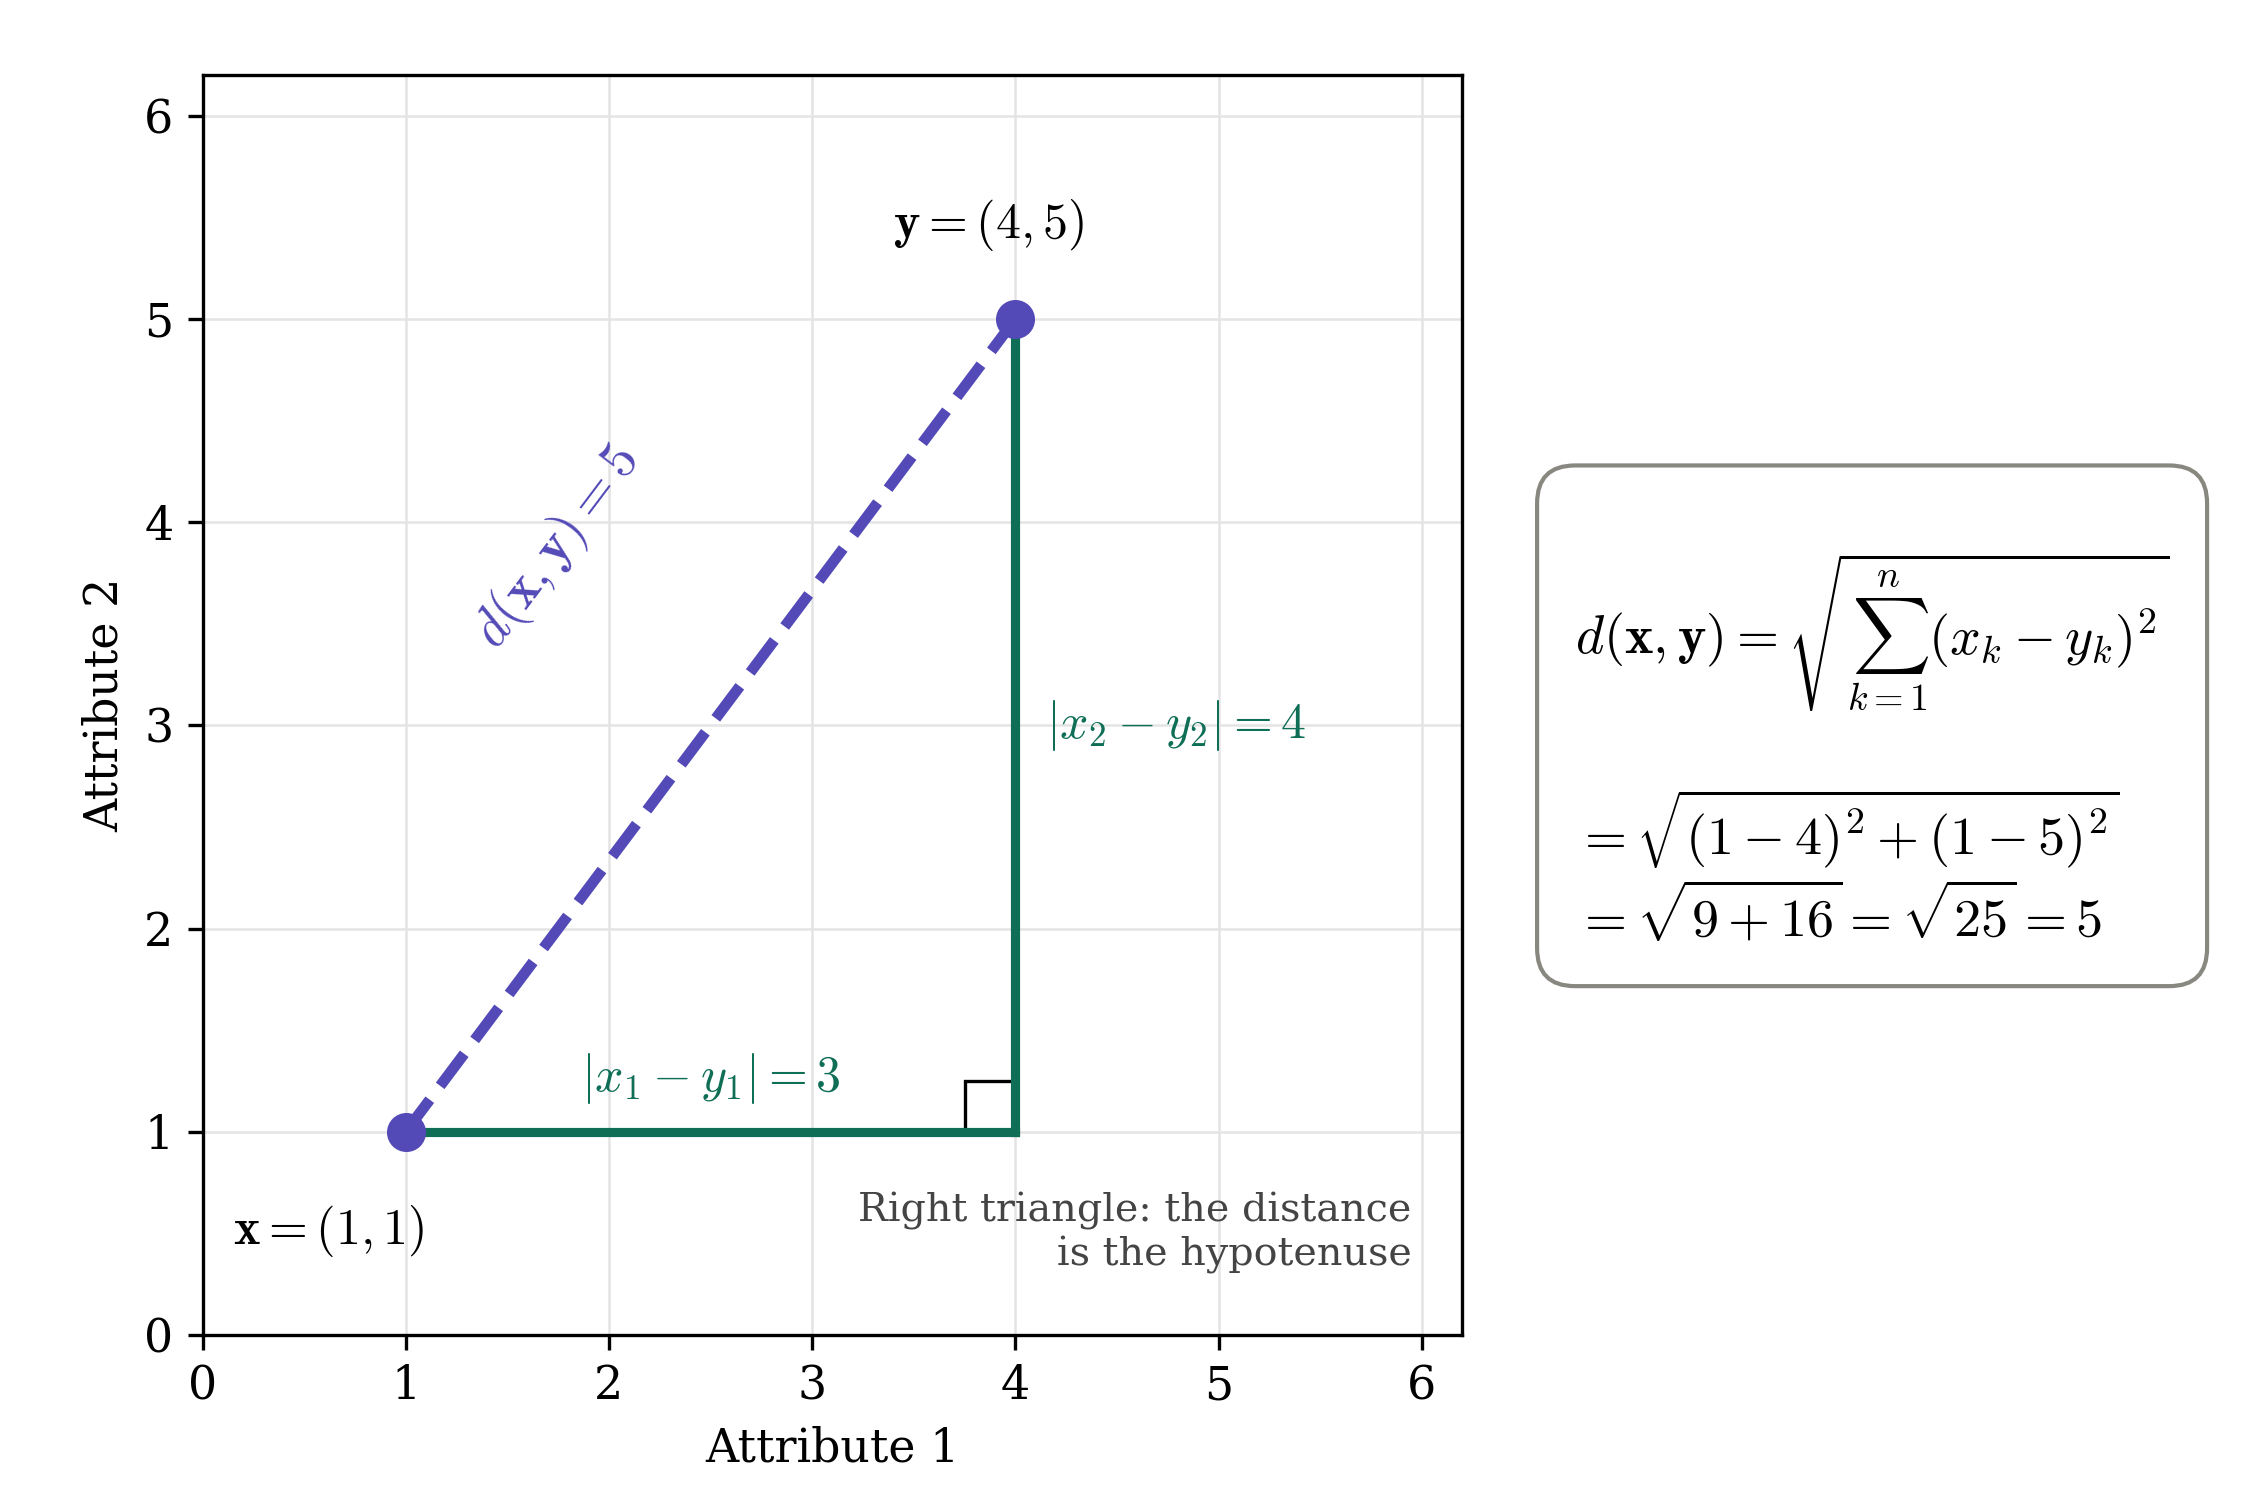
\includegraphics[width=0.5\textwidth]{images/chapter_3/euclidean_distance.png}
    \caption{Euclidean distance between $\mathbf{x}=(1,1)$ and $\mathbf{y}=(4,5)$: the per-attribute differences are the legs of a right triangle and the distance is its hypotenuse.}
\end{figure}

\begin{figure}[h]
    \centering
    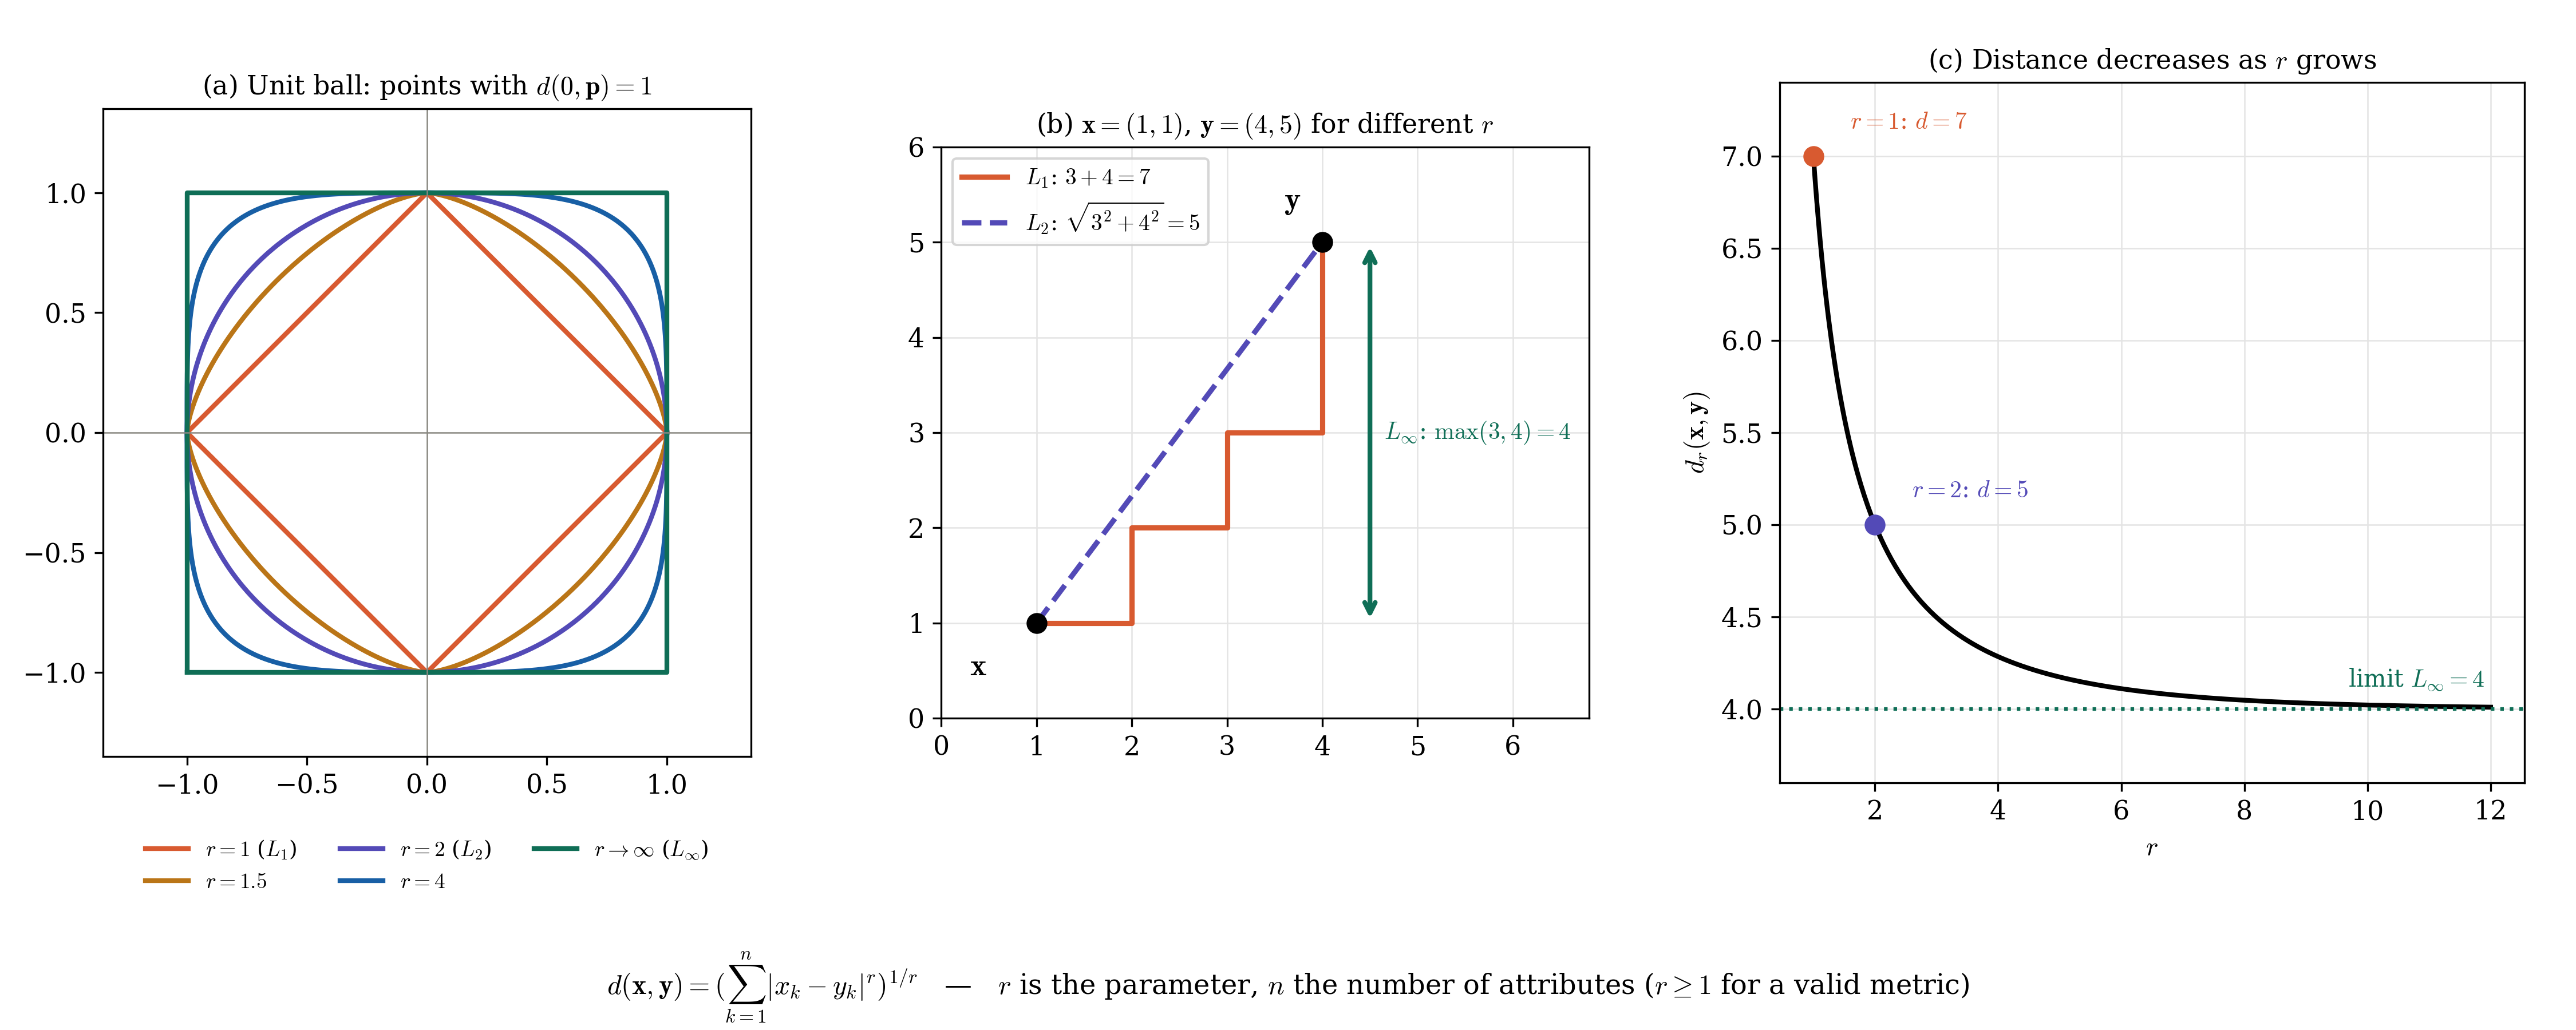
\includegraphics[width=0.5\textwidth]{images/chapter_3/minkowski_distance.png}
    \caption{Minkowski distance. (a) Unit ball for different values of $r$: a diamond for $L_1$, a circle for $L_2$, a square for $L_\infty$. (b) Distance between $\mathbf{x}=(1,1)$ and $\mathbf{y}=(4,5)$: $L_1=7$ (sum of differences), $L_2=5$ (straight line), $L_\infty=4$ (maximum difference). (c) The distance decreases as $r$ grows and converges to $L_\infty$.}
\end{figure}

\noindent\textbf{Note:} if attributes have very different scales (e.g.\ income in euros and age in years), the attribute with the largest range dominates the distance. For this reason, attributes are usually standardized before computing these distances.

\subsection{Properties of a Distance Metric}
A distance $d$ is called a \textbf{metric} if it satisfies the following properties for all points $x, y, z$ of the space:
\begin{itemize}
    \item \textbf{Identity:} the distance from a point to itself is zero: $d(x,x)=0$.
    \item \textbf{Positivity:} the distance between two distinct points is strictly positive: if $x\neq y$, then $d(x,y)>0$. Together with identity, this means that $d(x,y)=0$ if and only if $x=y$.
    \item \textbf{Symmetry:} the order of the points does not matter: $d(x,y)=d(y,x)$.
    \item \textbf{Triangle Inequality:} going directly from $x$ to $z$ is never longer than passing through an intermediate point $y$: $d(x,z)\le d(x,y)+d(y,z)$.
\end{itemize}

\begin{figure}[h]
    \centering
    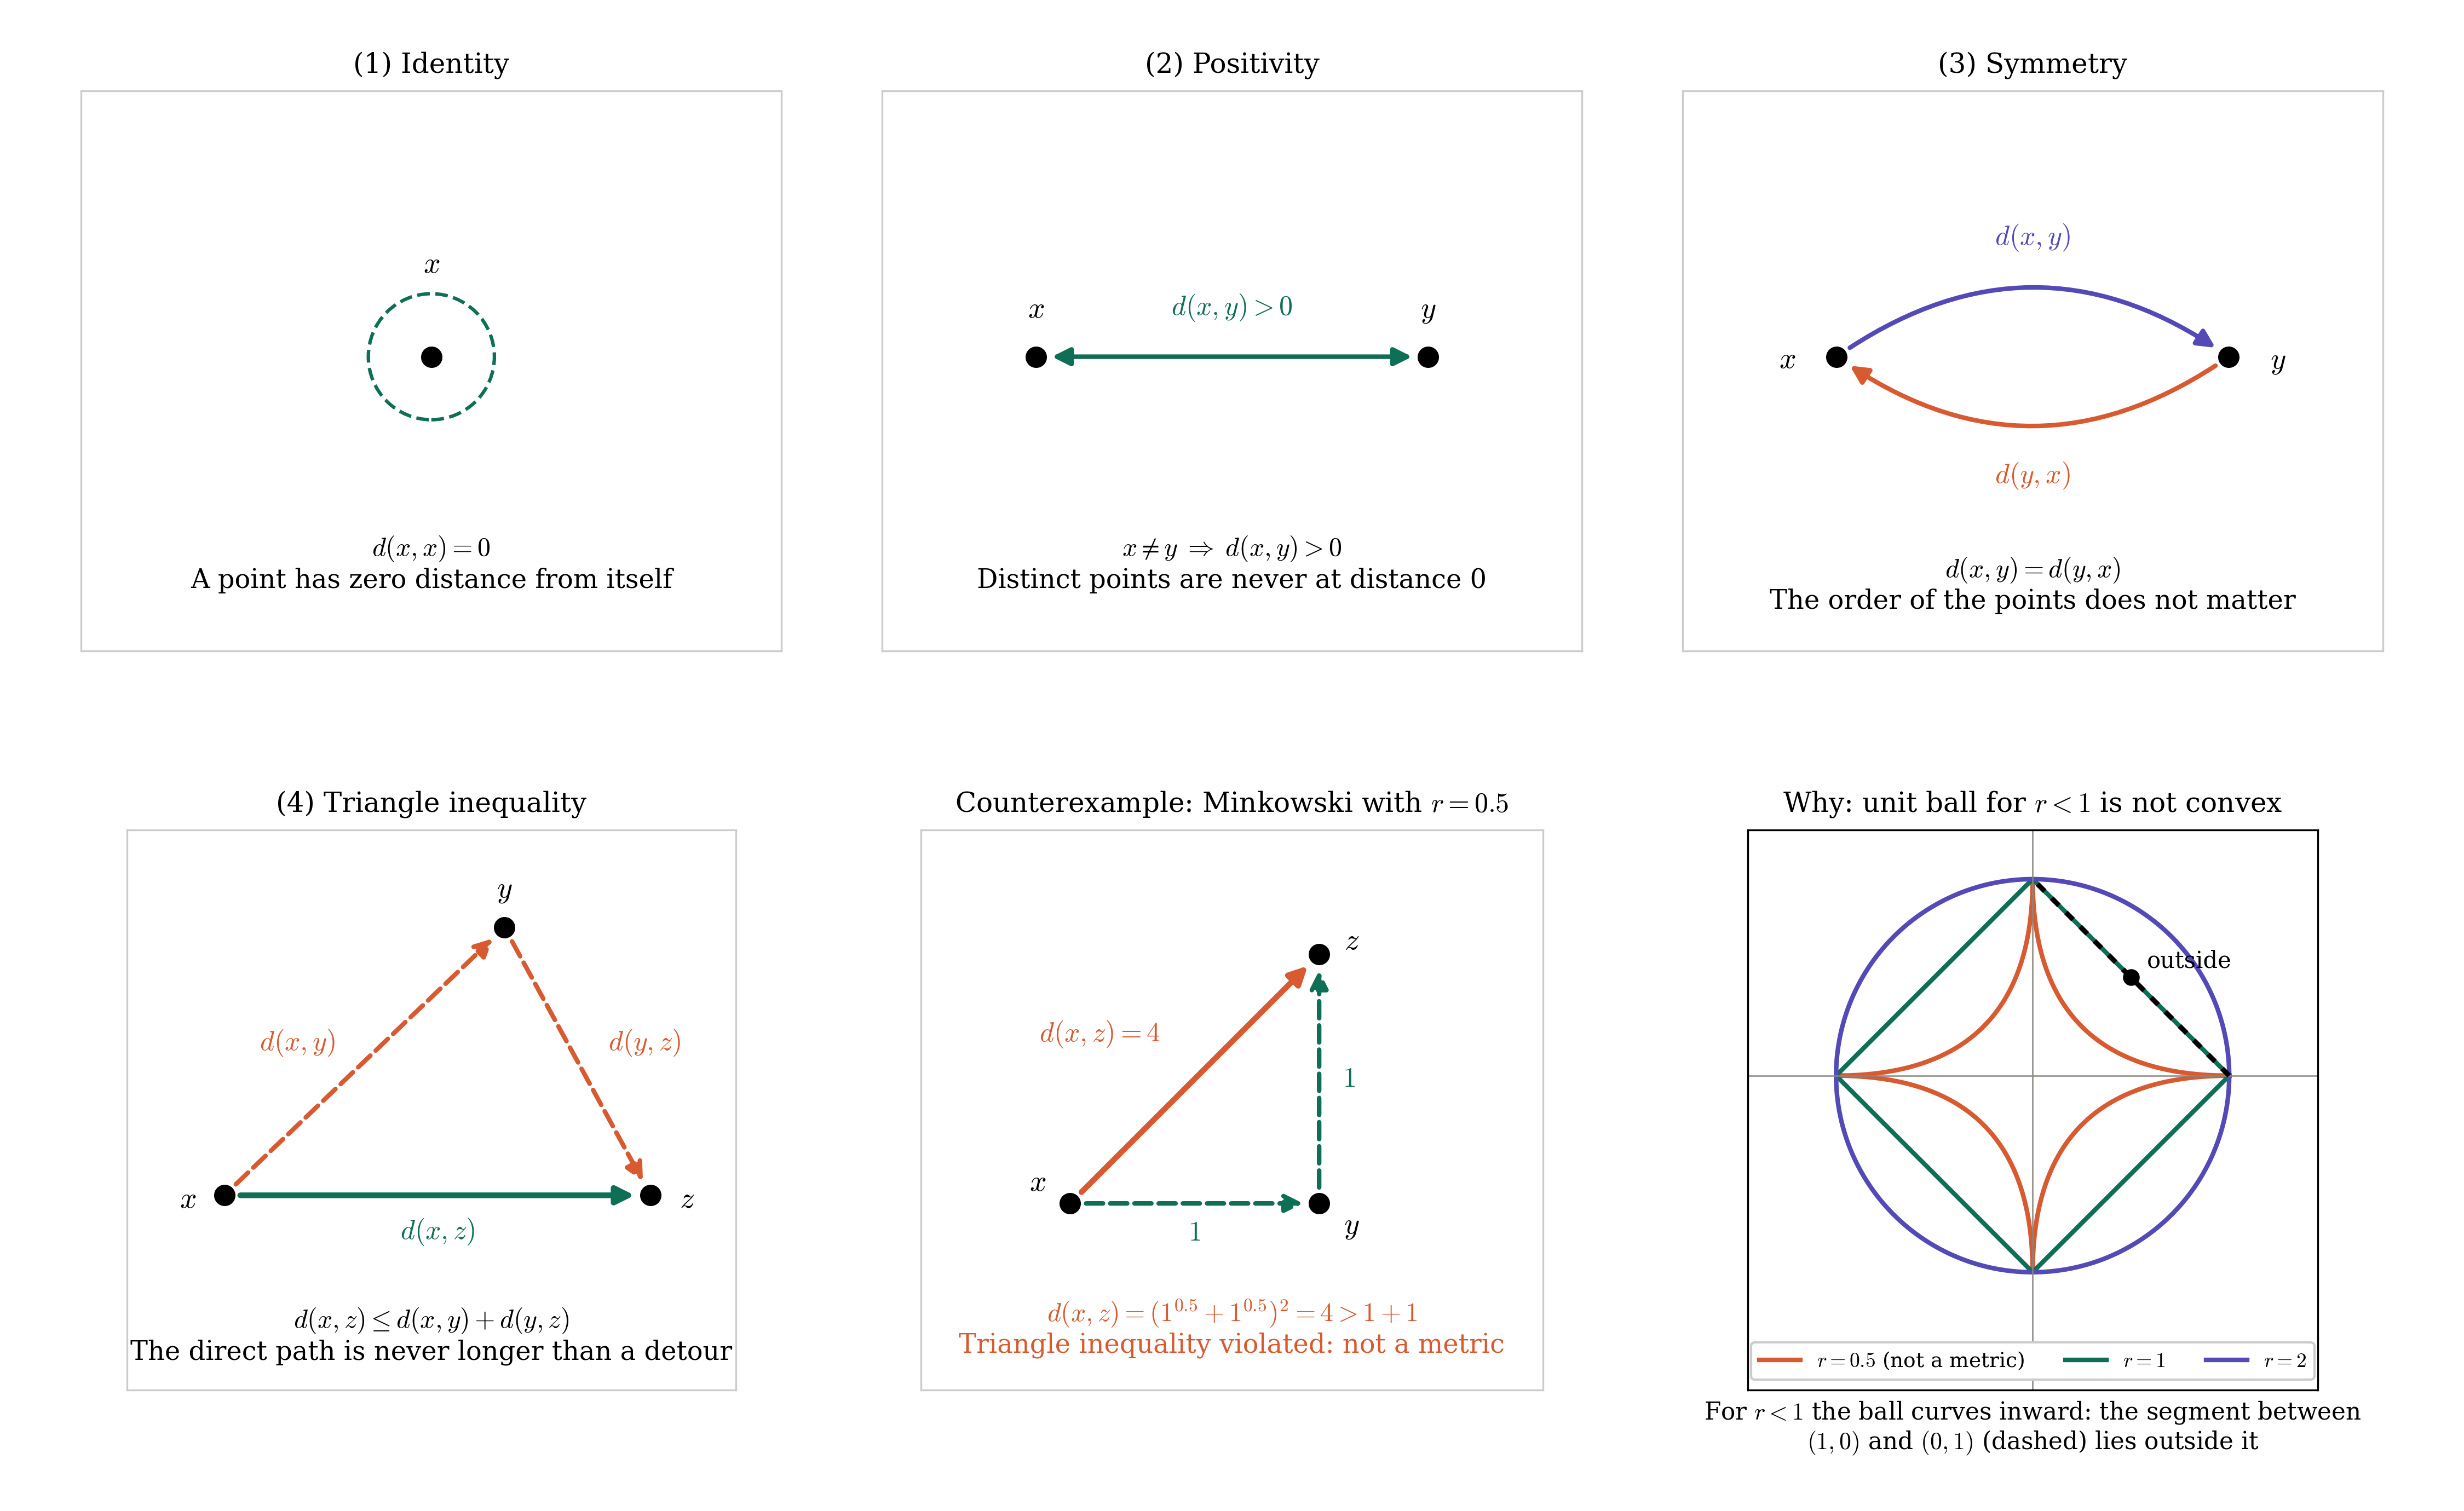
\includegraphics[width=0.8\textwidth]{images/chapter_3/distance_metric_properties.png}
    \caption{Properties of a distance metric. (1)--(4) The four properties: identity, positivity, symmetry and triangle inequality. Bottom centre: the Minkowski distance with $r=0.5$ violates the triangle inequality, since $d(x,z)=4>d(x,y)+d(y,z)=2$. Bottom right: for $r<1$ the unit ball is not convex, which is the geometric reason why the triangle inequality fails.}
\end{figure}

The Minkowski distance is a metric for every $r\geq1$. For $r<1$ the triangle inequality is violated: for instance, with $r=0.5$, $x=(0,0)$, $z=(1,1)$ and $y=(1,0)$ we get $d(x,z)=(1+1)^2=4$, while $d(x,y)+d(y,z)=1+1=2$, so the direct path would be longer than the detour.

\subsection{Mahalanobis Distance}
The Mahalanobis distance measures the distance between two points while taking into account the distribution of the data, described by its covariance matrix $S$:
\[
    d(\mathbf{x},\mathbf{y};S)=\sqrt{(\mathbf{x}-\mathbf{y})^\top S^{-1}(\mathbf{x}-\mathbf{y})}
\]
The inverse covariance matrix $S^{-1}$ reweights the differences between the points:

\begin{itemize}
    \item along directions where the data have \textbf{high variance}, a difference counts \emph{less}, because large spreads are normal there;
    \item along directions where the data have \textbf{low variance}, the same difference counts \emph{more}, because it is unusual;
    \item \textbf{correlations} between attributes are also taken into account, so redundant information is not counted twice.
\end{itemize}

As a consequence, the Mahalanobis distance is unitless and scale-invariant. Two special cases help to interpret it:

\begin{figure}[h]
    \centering
    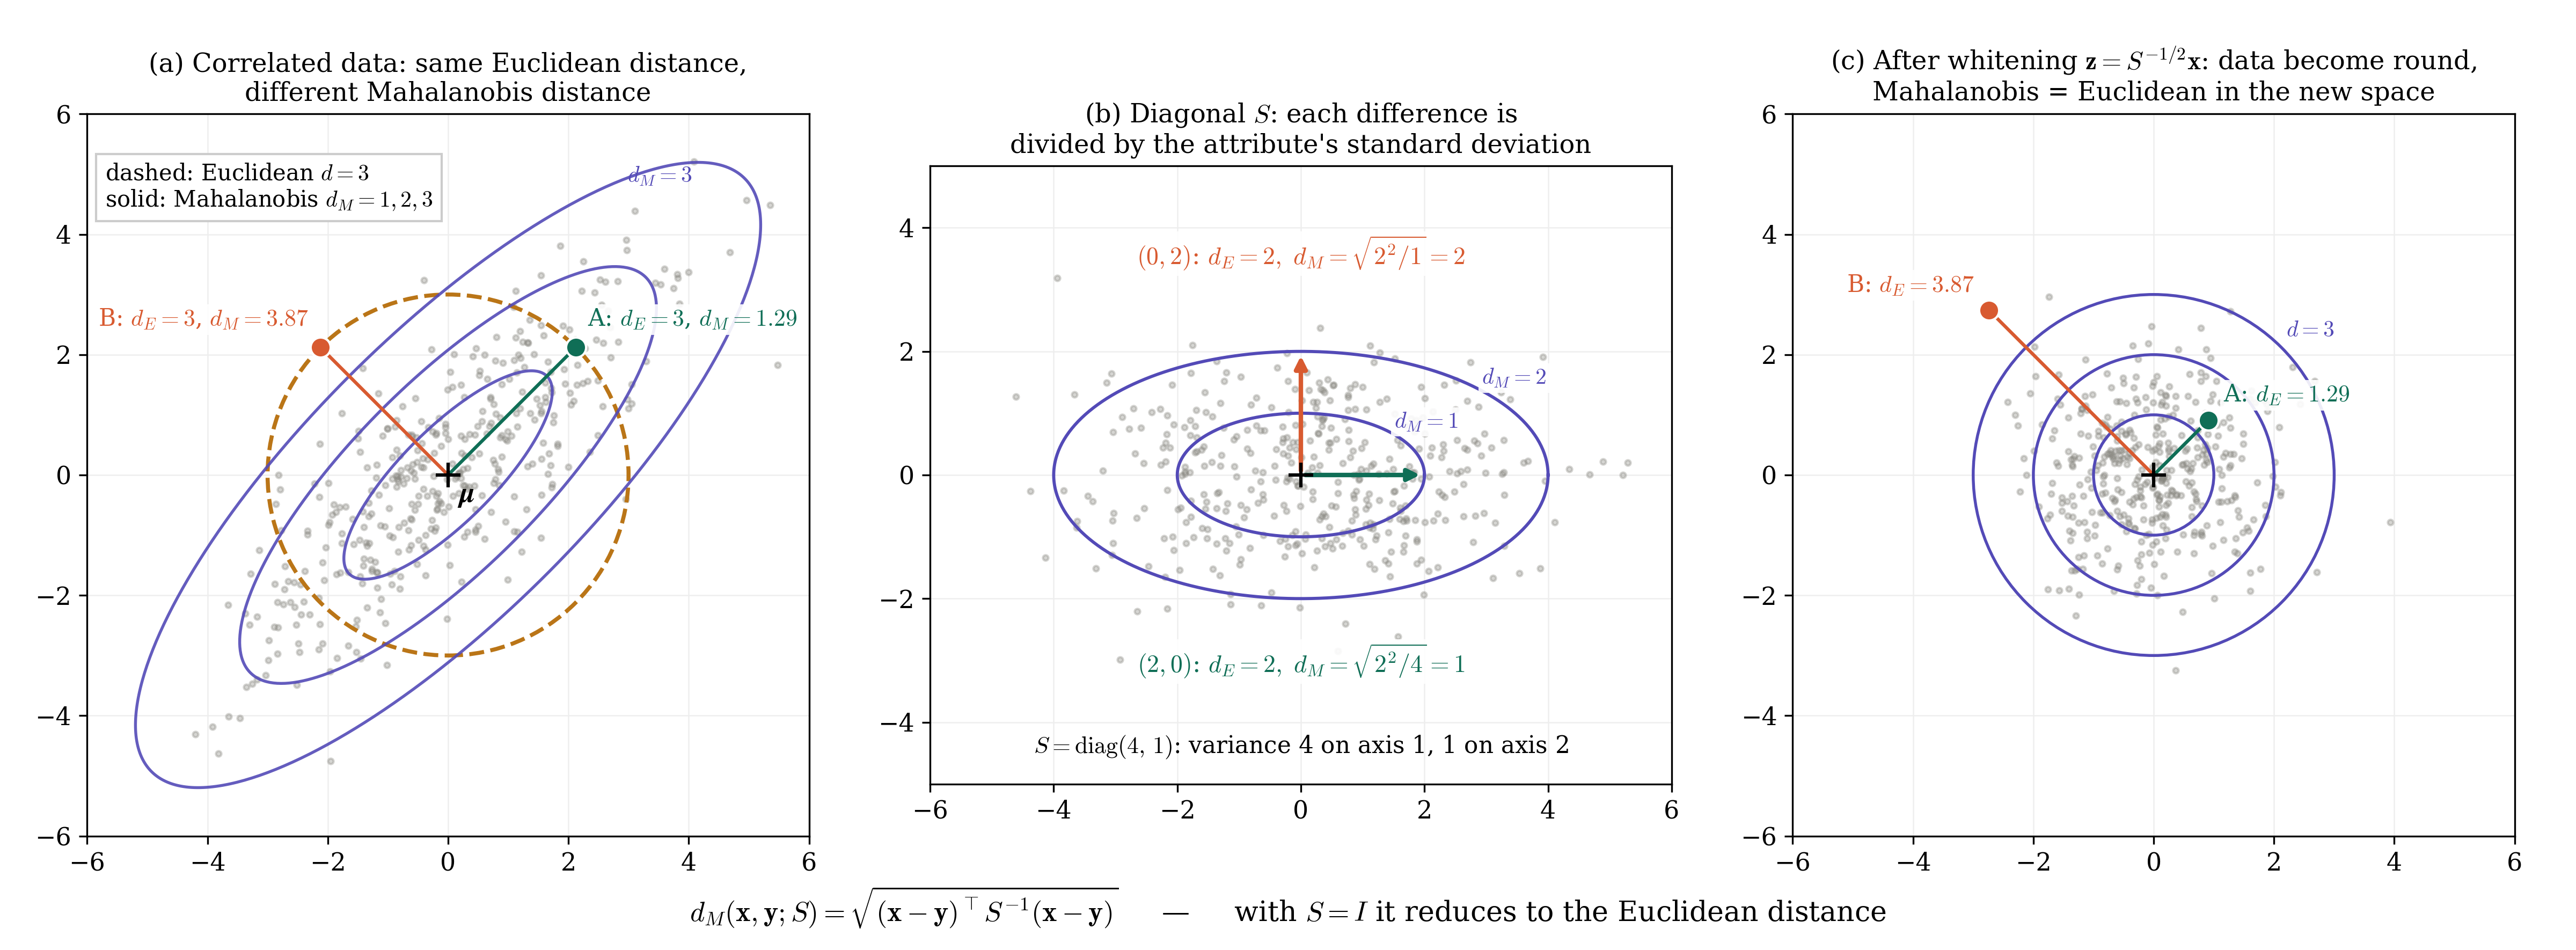
\includegraphics[width=0.8\textwidth]{images/chapter_3/mahalanobis_distance.png}
    \caption{Mahalanobis distance. (a) With correlated data, points A and B have the same Euclidean distance from the mean $\boldsymbol{\mu}$, but A lies along the direction of high variance ($d_M=1.29$) while B lies across it ($d_M=3.87$): the contours of constant Mahalanobis distance are ellipses that follow the shape of the data. (b) With a diagonal $S$ each difference is divided by the standard deviation of its attribute: the same Euclidean difference of $2$ gives $d_M=1$ along the high-variance axis and $d_M=2$ along the low-variance one. (c) Transforming the data with $S^{-1/2}$ (whitening) makes the distribution round, and the Euclidean distance in the new space equals the Mahalanobis distance in the original one.}
\end{figure}

\begin{itemize}
    \item if $S=I$ (identity matrix: unit variances and no correlation), it reduces to the \textbf{Euclidean distance};
    \item if $S$ is diagonal, it is equivalent to the Euclidean distance computed on \textbf{standardized} attributes, i.e.\ each difference is divided by the standard deviation of its attribute.
\end{itemize}
\textbf{Example:} let $S=\begin{pmatrix}4&0\\0&1\end{pmatrix}$, so the first attribute has variance $4$ and the second variance $1$. For a difference $\mathbf{x}-\mathbf{y}=(2,0)$ we get $d=\sqrt{2^2/4}=1$, while for $\mathbf{x}-\mathbf{y}=(0,2)$ we get $d=\sqrt{2^2/1}=2$. Both pairs have Euclidean distance $2$, but the Mahalanobis distance considers the second pair farther apart, since a difference of $2$ is much less common along the second attribute.

\section{Data PreProcessing}
Real-world data are rarely ready to be analysed: they can be noisy, redundant, too large, described by too many attributes, or stored in formats that algorithms cannot handle (e.g.\ text). \textbf{Data PreProcessing} is the set of techniques that turn raw data into a form that is cleaner, smaller and more suitable for the analysis. The main techniques are:
\begin{itemize}
    \item \textbf{Data Aggregation:} combining two or more attributes or objects into a single one.
    \item \textbf{Data Reduction:} obtaining a smaller dataset that gives (almost) the same analytical results.
    \item \textbf{Feature Selection:} keeping only the useful attributes, needed to tackle the \emph{curse of dimensionality} (Section~\ref{sec:curse}).
    \item \textbf{Feature Transformation or Normalization:} changing the values or the scale of attributes (Sections~\ref{sec:transformation}--\ref{sec:attr-transformation}).
    \item \textbf{Preprocessing for textual data:} turning documents into structured data (Section~\ref{sec:documents}).
\end{itemize}

\paragraph{Data Aggregation.} Aggregation replaces a group of objects (or attributes) with a single one that summarises them, typically with a sum or an average. Examples: daily sales $\rightarrow$ monthly sales, cities $\rightarrow$ regions, single transactions $\rightarrow$ total per customer. It is used for three purposes:
\begin{itemize}
    \item \textbf{data reduction:} fewer objects to store and process (365 days become 12 months);
    \item \textbf{change of scale:} looking at the data at a coarser level of detail (regions instead of cities);
    \item \textbf{more stable data:} averages vary less than single values, because random fluctuations tend to cancel out (Figure~\ref{fig:aggregation}).
\end{itemize}
The price to pay is the loss of detail: after aggregating into months, it is no longer possible to know what happened on a specific day.

\begin{figure}[htbp]
    \centering
    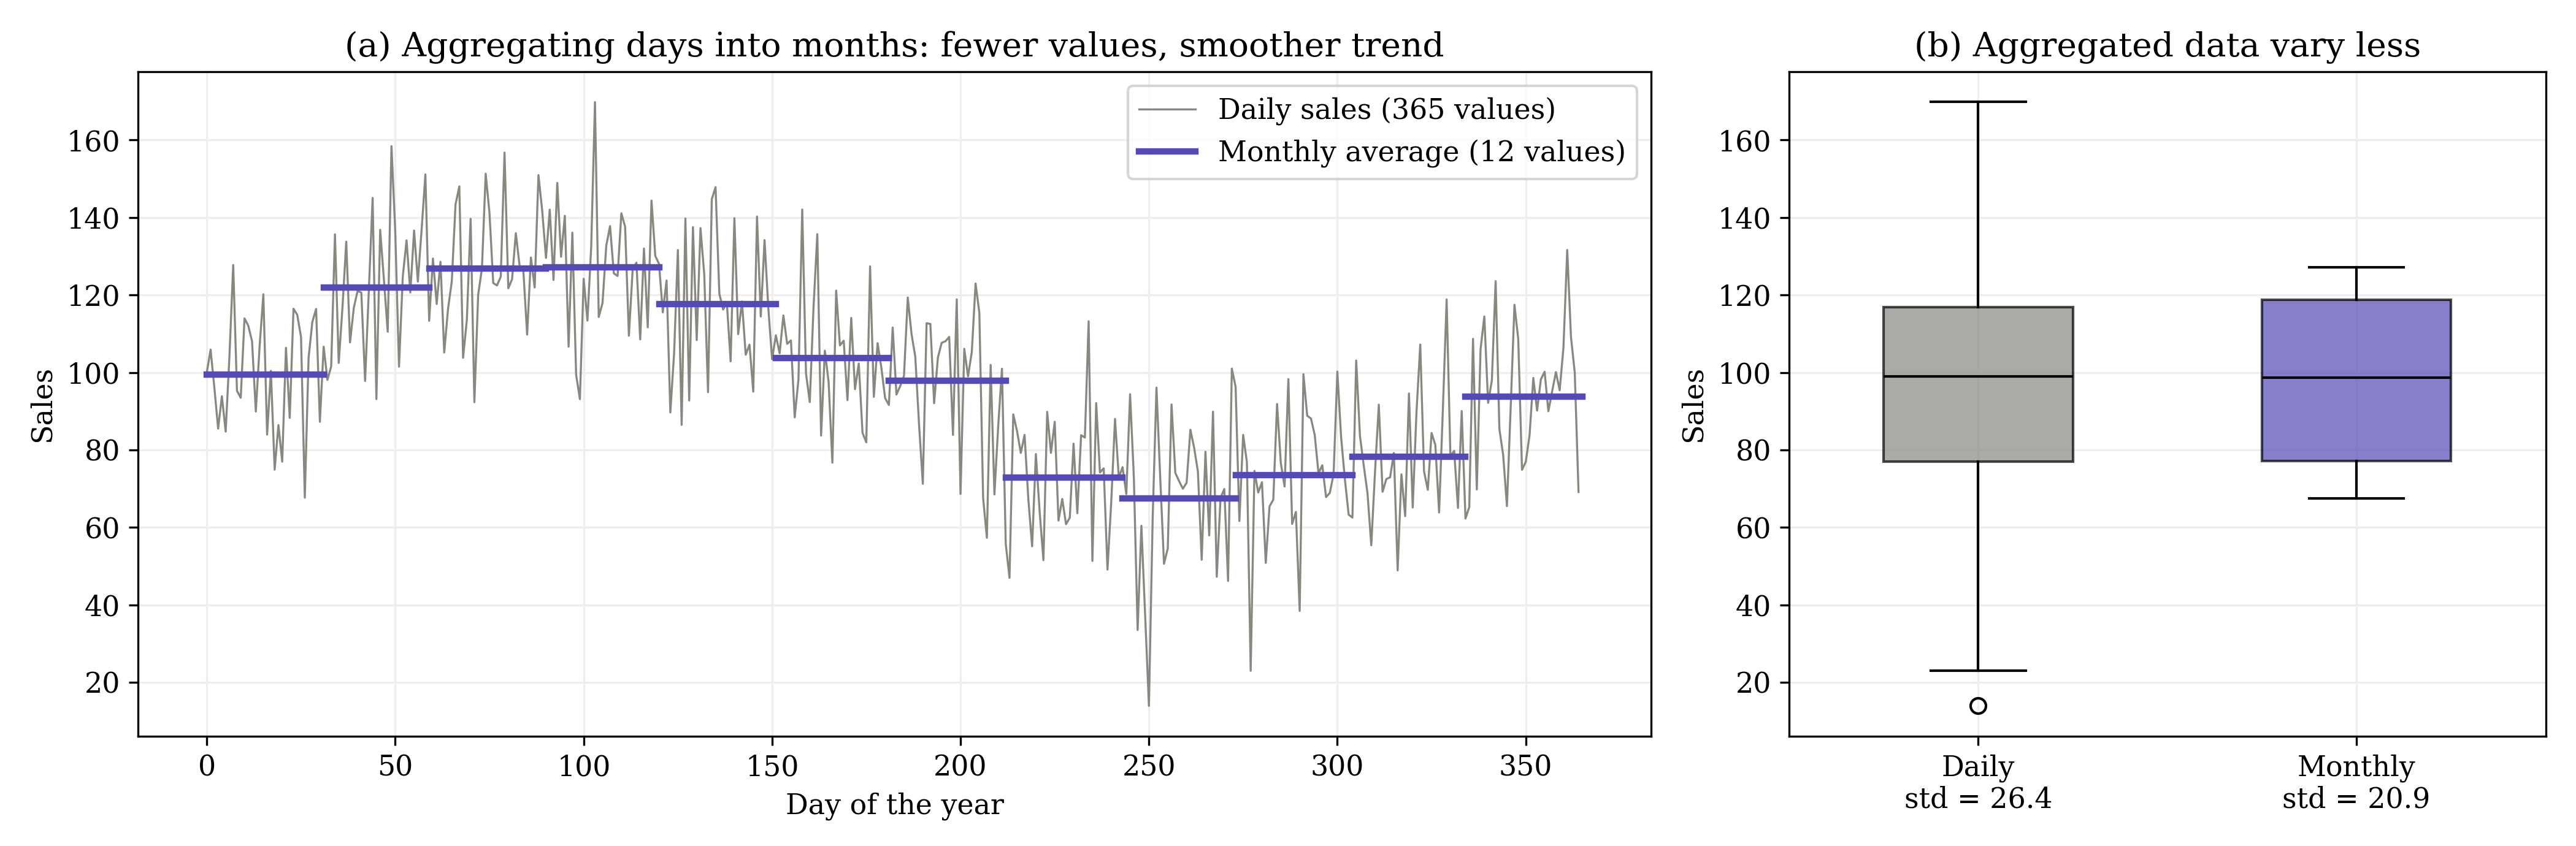
\includegraphics[width=0.8\textwidth]{images/chapter_3/aggregation.png}
    \caption{Data aggregation. (a) 365 daily values are replaced by 12 monthly averages, which show the trend more clearly. (b) The aggregated values have a lower variability (smaller standard deviation) than the original ones.}
\end{figure}

\paragraph{Data Reduction.} Data reduction generates a reduced representation of the dataset, \emph{smaller in volume but able to provide similar analytical results}. A dataset is a table, so it can be reduced along three directions:
\begin{itemize}
    \item \textbf{fewer rows}, i.e.\ fewer objects: \emph{sampling} (reduces the cardinality of the dataset);
    \item \textbf{fewer columns}, i.e.\ fewer attributes: \emph{feature selection and creation};
    \item \textbf{fewer distinct values per column}: \emph{discretization} (reduces the cardinality of the attribute domains, e.g.\ age $\rightarrow$ \{young, adult, senior\}).
\end{itemize}

\paragraph{Sampling.} Sampling is the main technique for data selection and reduction: instead of analysing all the objects, only a subset of them (the \emph{sample}) is analysed. It is useful when processing the whole dataset is too expensive or too slow. It is based on two key principles:
\begin{itemize}
    \item using a sample works almost as well as using the entire dataset, \emph{if the sample is representative};
    \item a sample is \textbf{representative} if it has approximately the same property of interest as the original dataset (e.g.\ the same mean, or the same proportion of each class).
\end{itemize}
There are two main types of sampling:
\begin{itemize}
    \item \textbf{Simple Random Sampling:} every object has the same probability of being selected. It is simple, but with small samples or rare classes it may produce an unrepresentative sample by chance: a class that is $10\%$ of the data could be missing entirely (Figure~\ref{fig:sampling}b).
    \item \textbf{Stratified Sampling:} the data are first split into groups (\emph{strata}), for instance one per class, and then a random sample is drawn from each group, proportionally to its size. This guarantees that every group is represented with the right proportion (Figure~\ref{fig:sampling}c).
\end{itemize}

\begin{figure}[htbp]
    \centering
    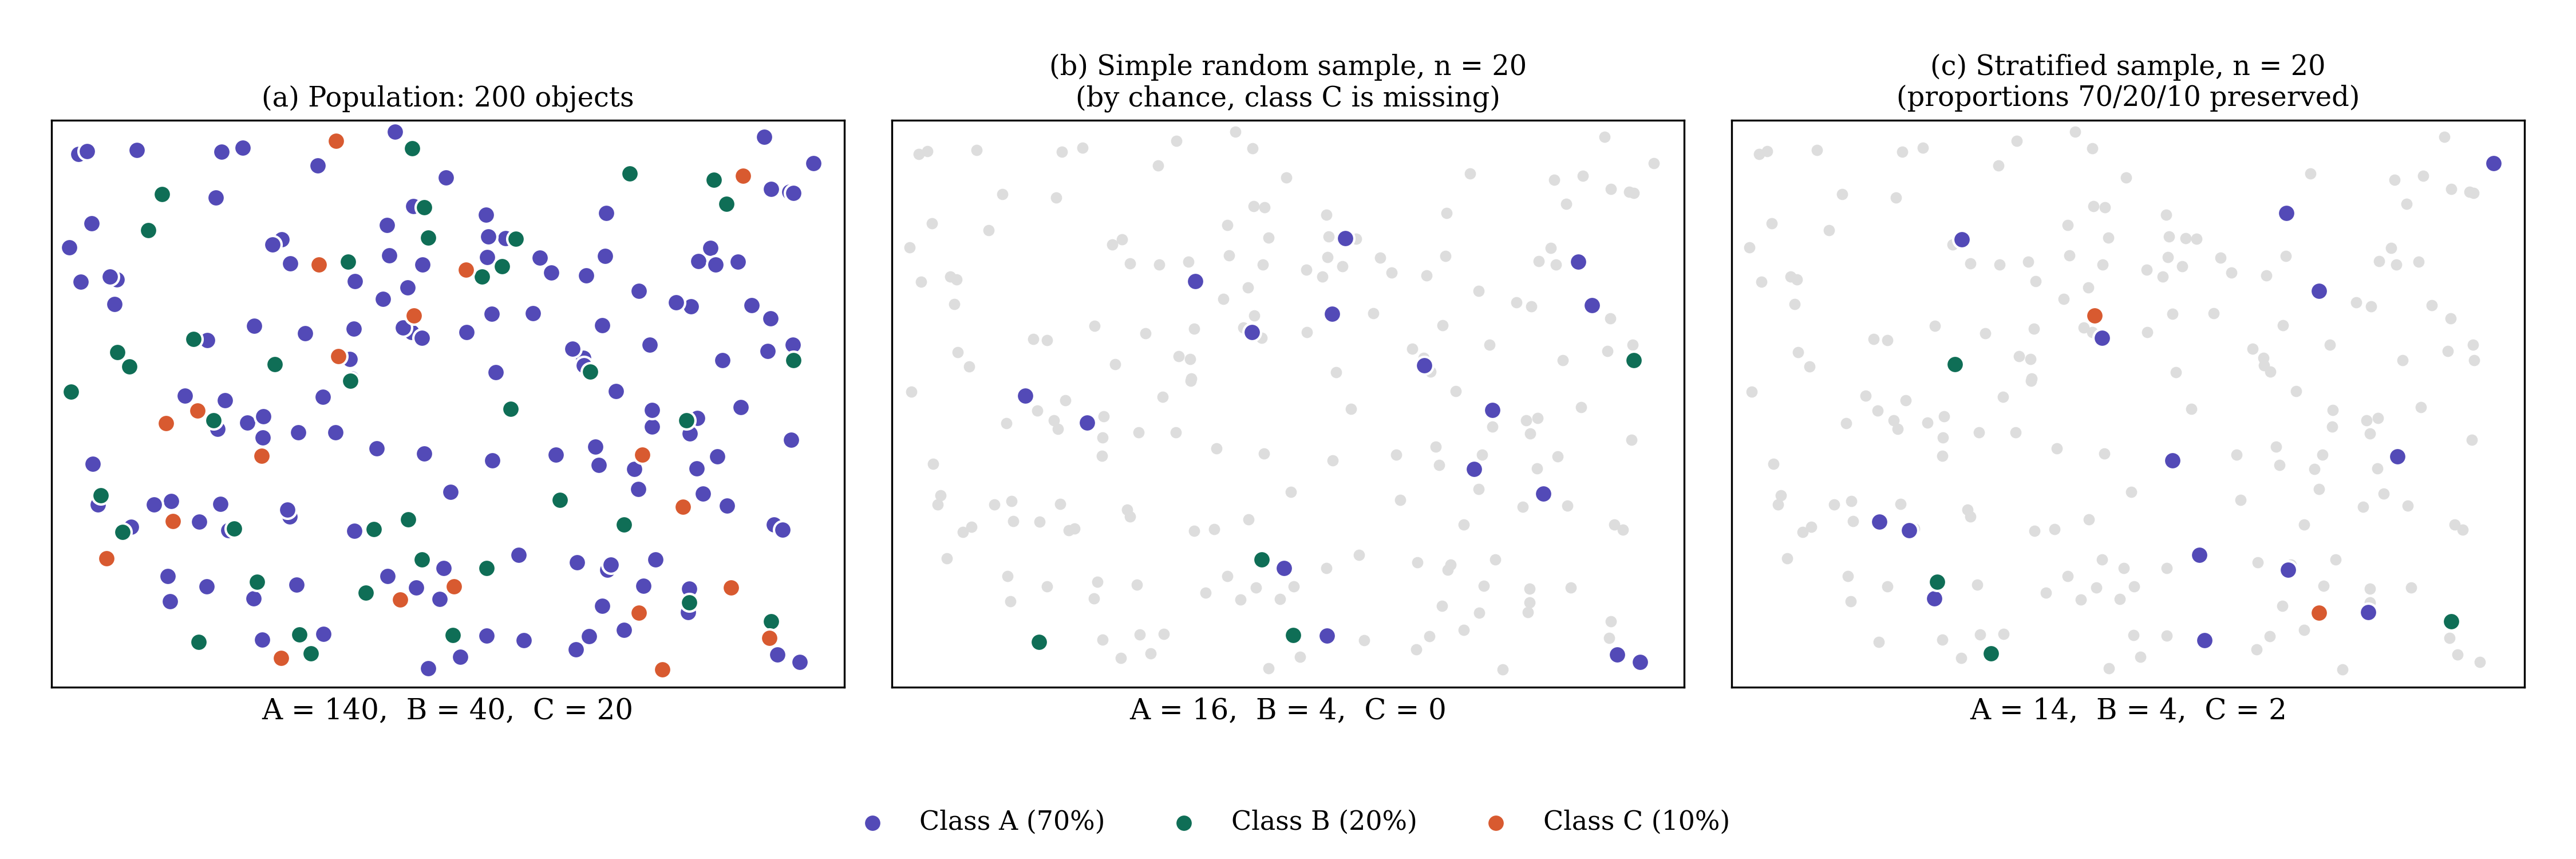
\includegraphics[width=0.8\textwidth]{images/chapter_3/sampling.png}
    \caption{Sampling 20 objects from a population of 200 with imbalanced classes (70\%, 20\%, 10\%). Simple random sampling may miss the rarest class, while stratified sampling preserves the original proportions.}
\end{figure}

\subsection{Curse of Dimensionality}
The \textbf{curse of dimensionality} is the set of problems that arise when the number of attributes (dimensions) becomes large. The key idea is simple: \emph{when the number of dimensions increases, the volume of the space grows so fast that the data become sparse}, i.e.\ points are far from each other and the space is mostly empty.

Two effects make this concrete (Figure~\ref{fig:curse}):
\begin{itemize}
    \item \textbf{Neighbourhoods are no longer local.} With uniform data in a unit cube, a sub-cube that contains $10\%$ of the points has edge $0.1$ in 1 dimension, but edge $0.79$ in 10 dimensions: to find ``nearby'' points one must cover almost the whole range of every attribute.
    \item \textbf{Distances become all similar.} As the dimensions grow, the distance to the nearest point and the distance to the farthest point become almost the same. If all points are roughly equally distant, the concept of ``near'' loses its meaning.
\end{itemize}
As a consequence, the definitions of \textbf{density} and \textbf{distance} between points, which are critical for clustering and outlier detection, become less meaningful.

\begin{figure}[htbp]
    \centering
    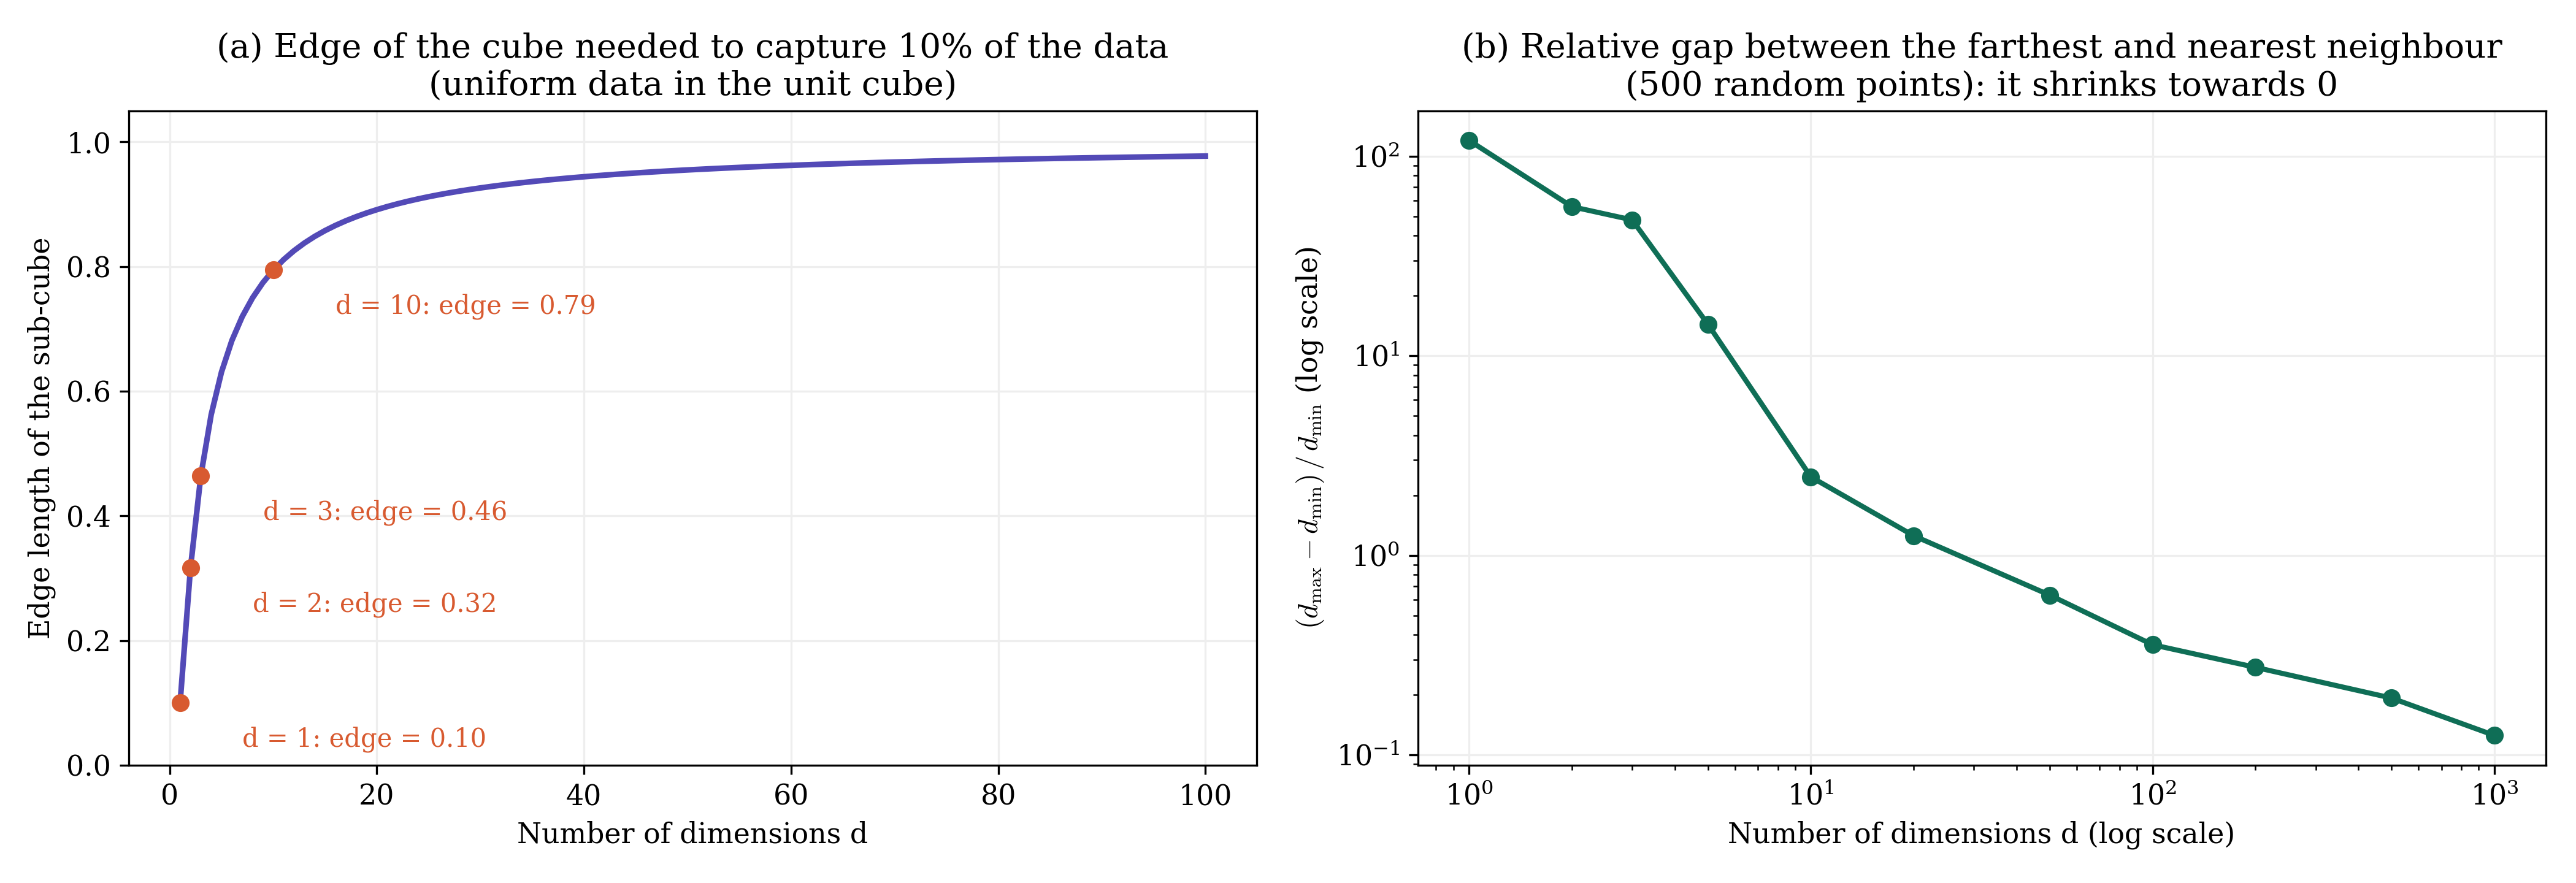
\includegraphics[width=0.8\textwidth]{images/chapter_3/curse_of_dimensionality.png}
    \caption{Curse of dimensionality. (a) To capture 10\% of uniformly distributed data, the edge of the sub-cube quickly approaches the full range as the number of dimensions grows. (b) The relative difference between the farthest and the nearest neighbour shrinks towards zero: in high dimensions all points look equally distant.}
\end{figure}

\paragraph{Feature Subset Selection.} One way to counter the curse of dimensionality is to keep only a subset of the attributes. Feature Subset Selection reduces the dimensionality of the data by removing:
\begin{itemize}
    \item \textbf{redundant features}, which duplicate much or all of the information contained in other attributes. Example: the price of a product with and without VAT; knowing one, the other adds nothing.
    \item \textbf{irrelevant features}, which contain no useful information for the task at hand. Example: the student ID when predicting the student's grade.
\end{itemize}

\paragraph{Recursive Feature Elimination (RFE).} A common way to perform feature selection is to remove features one step at a time, always discarding the least useful one (Figure~\ref{fig:rfe}):
\begin{enumerate}
    \item assign a weight (importance) to each feature, for instance the absolute value of the coefficients of a linear model;
    \item train the model (\emph{estimator}) on the current set of features and obtain the importance of each feature;
    \item remove (\emph{prune}) the least important feature(s) from the current set;
    \item repeat steps 2--3 on the reduced set, until the desired number of features is reached.
\end{enumerate}
The model is retrained at every iteration because removing a feature can change the importance of the others. For the same reason, RFE can be expensive when there are many features.

\begin{figure}[htbp]
    \centering
    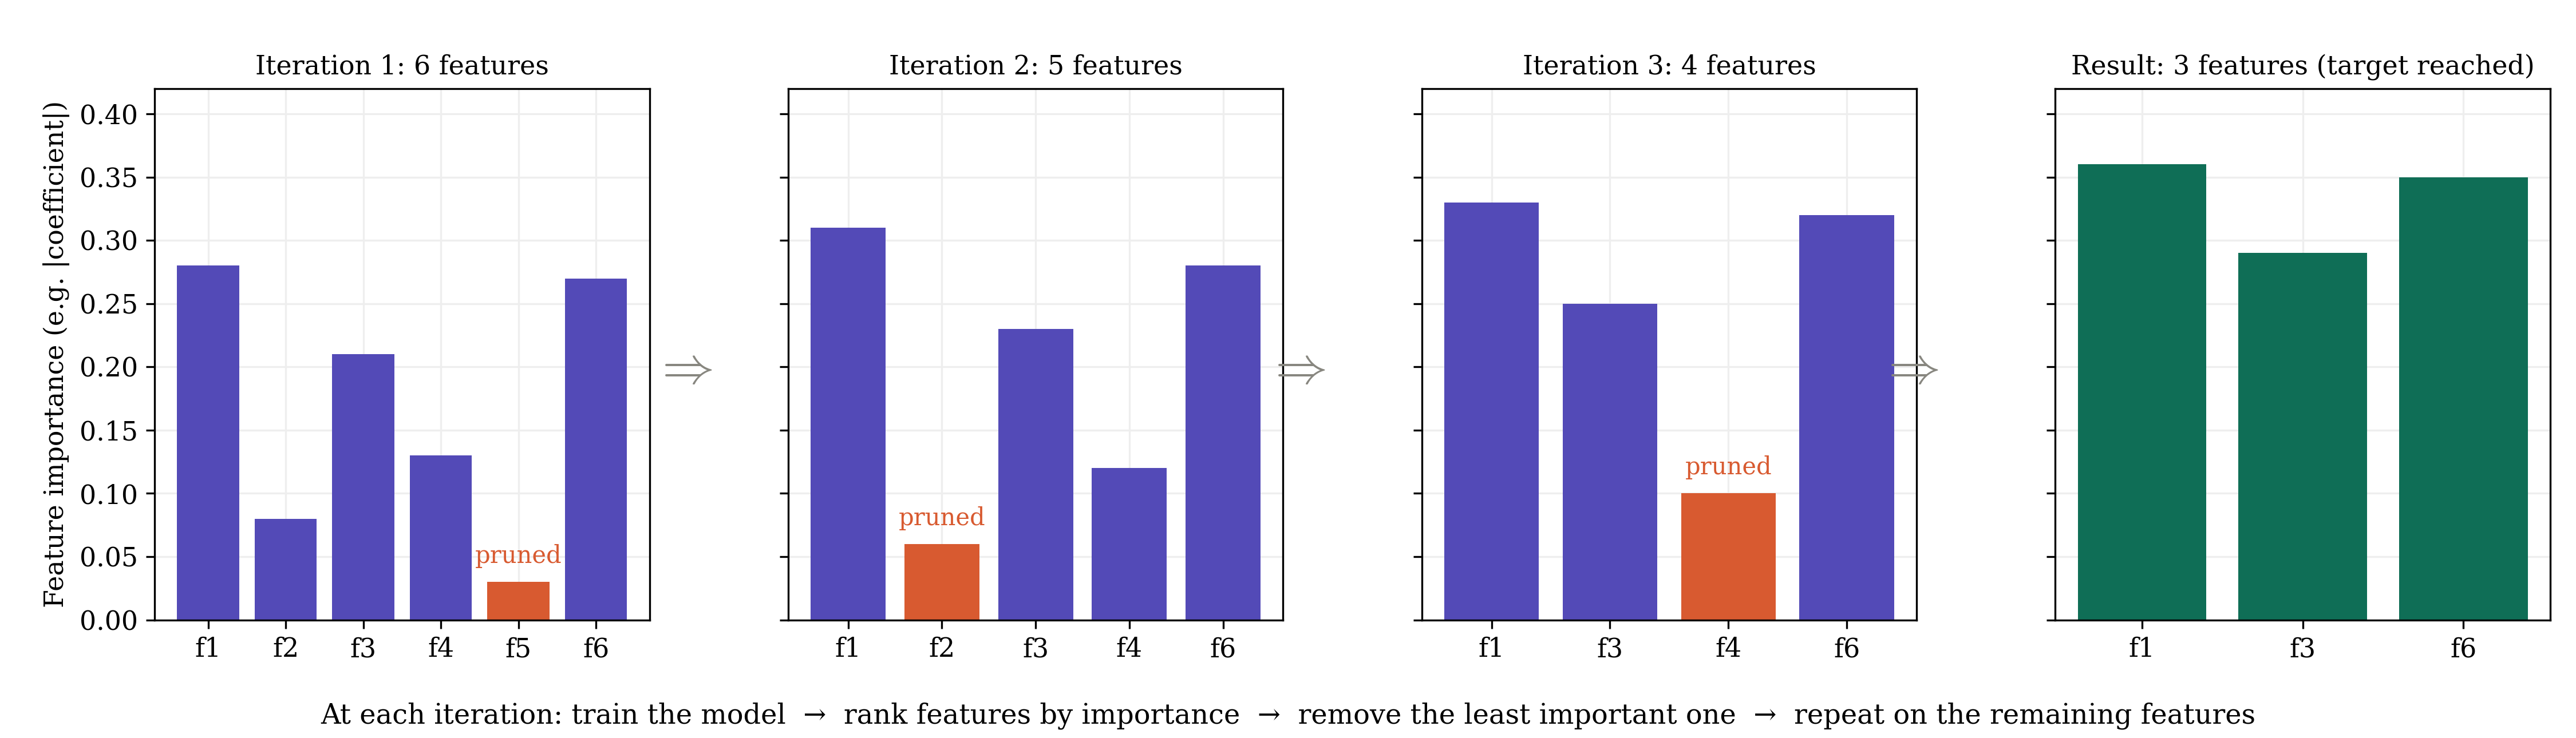
\includegraphics[width=0.8\textwidth]{images/chapter_3/rfe.png}
    \caption{Recursive Feature Elimination with a target of 3 features. At each iteration the model is retrained, the importances are recomputed and the least important feature (in orange) is removed.}
\end{figure}

\paragraph{Other approaches.}
\begin{itemize}
    \item \textbf{Feature importance of interpretable models:} some models directly tell how much each feature contributes to the prediction, for instance Decision Trees (how much each feature is used to split the data) and Linear Regression (the size of the coefficients, if the features are on the same scale). The least important features can then be discarded.
    \item \textbf{Decomposition techniques} such as PCA and SVD can be used to reduce dimensionality automatically. Strictly speaking, they do not select original features but \emph{create new ones}: each component is a combination of the original attributes, and the first few components capture most of the information in the data. Looking at how much each original attribute contributes to the main components also tells which attributes are the most important.
\end{itemize}

\subsection{Feature Engineering}
\textbf{Feature Engineering} is the act of extracting features from raw data and transforming them into formats that are more suitable for a Machine Learning model. A good representation of the data often matters more than the choice of the algorithm. Different techniques are needed according to the type of data:

\begin{center}
    \small
    \renewcommand{\arraystretch}{1.3}
    \begin{tabular}{|l|p{3.6cm}|p{5.2cm}|}
    \hline
    \textbf{Data type} & \textbf{Examples} & \textbf{Typical techniques} \\
    \hline
    Structured & numerical, categorical attributes & normalization, discretization, binarization (one-hot encoding) \\
    \hline
    Unstructured & text, images, signals & tokenization and term vectors, Fourier transform, extraction of descriptors \\
    \hline
    Mixed & e.g.\ a product with price, category and description & combination of the above \\
    \hline
    \end{tabular}
\end{center}

The basic Feature Engineering techniques, described in the next subsections, are \textbf{data transformation}, \textbf{discretization}, \textbf{binarization} and \textbf{normalization}.

\subsection{Data Transformation}
Data transformation is the process of converting data from one format or representation to another, so that the important information is captured much more efficiently than in the original representation.

The classic example is the \textbf{Fourier Transform}, which converts a signal from the \emph{time domain} (value at each instant) to the \emph{frequency domain} (which frequencies the signal contains, and how strong they are). A signal made of a few overlapping waves looks complicated as a sequence of values, but in the frequency domain it is summarised by a few peaks (Figure~\ref{fig:fourier}).

\begin{figure}[htbp]
    \centering
    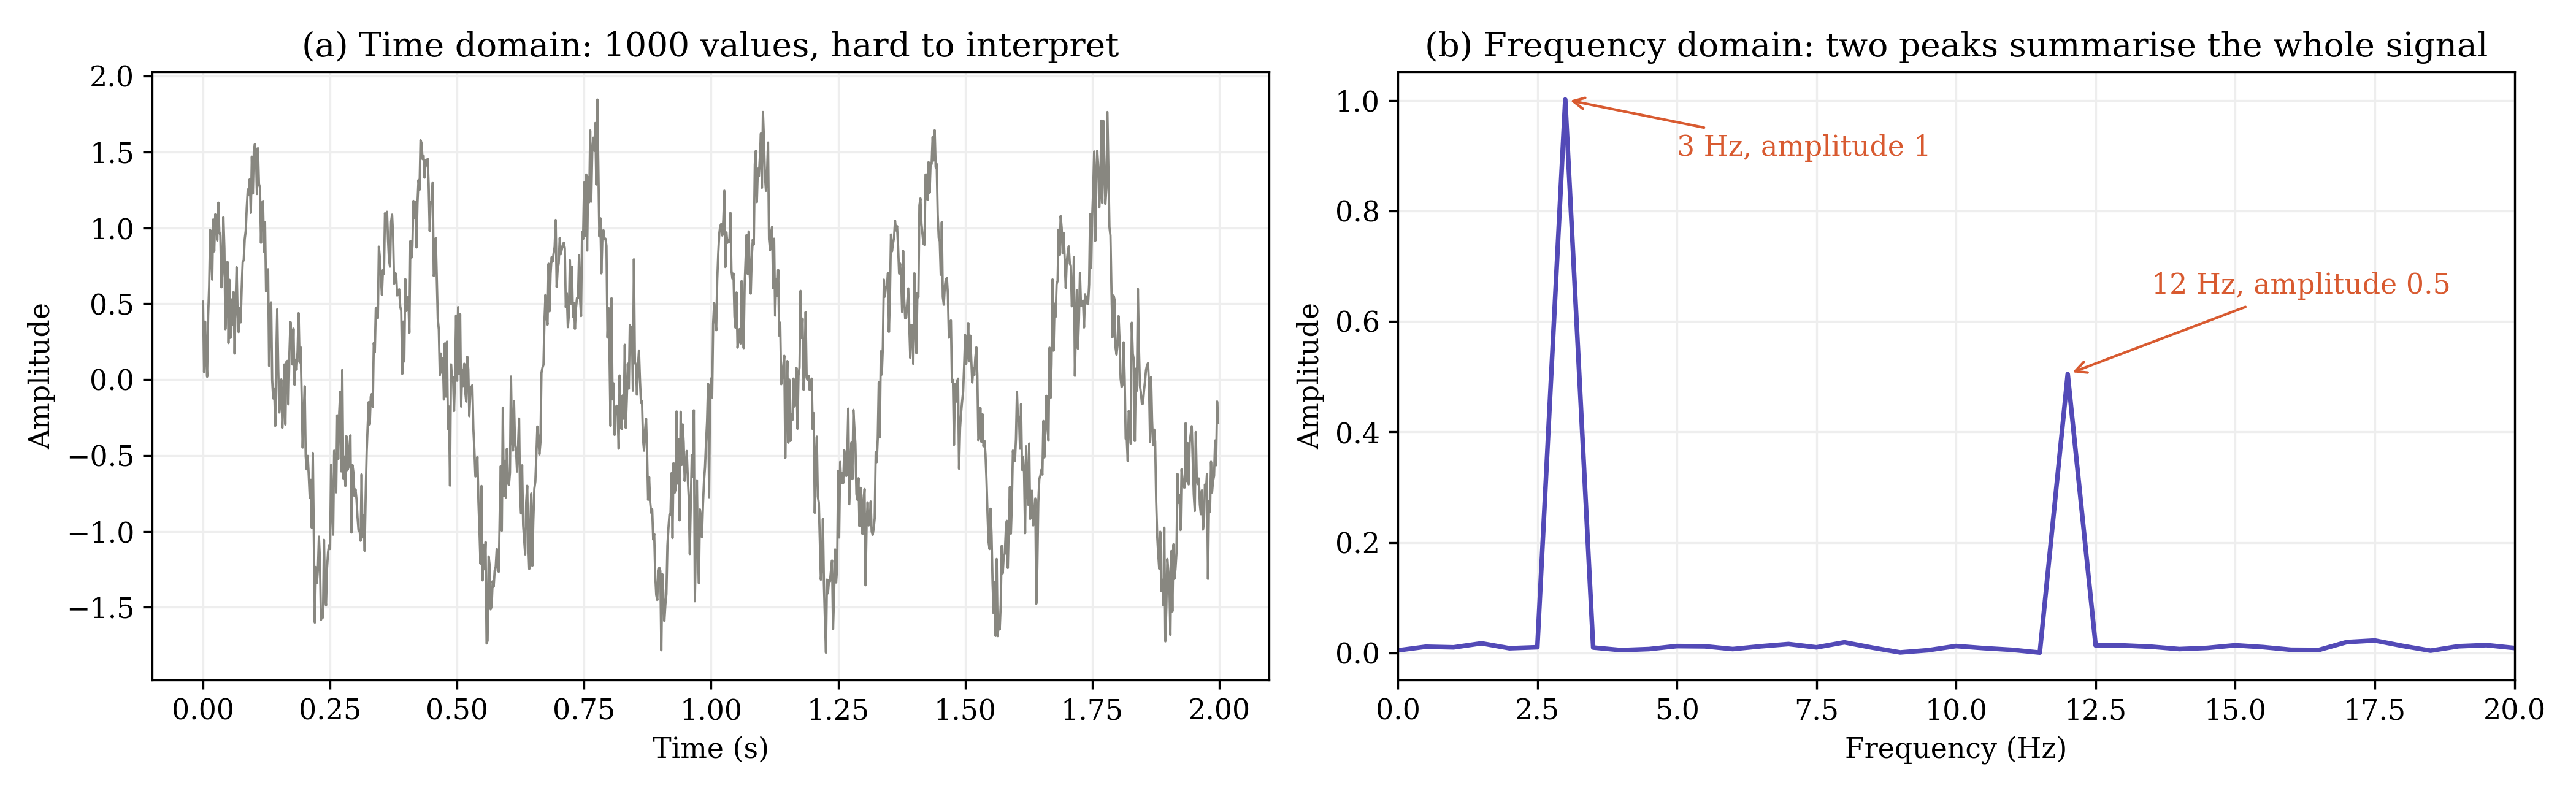
\includegraphics[width=0.8\textwidth]{images/chapter_3/fourier_transform.png}
    \caption{Fourier transform. (a) A noisy signal made of two waves (3\,Hz and 12\,Hz), represented by 1000 values over time. (b) The same signal in the frequency domain: two peaks describe it completely.}
\end{figure}

Another very common case is the conversion of \textbf{non-numerical data into numerical data}: most algorithms work only with numbers, so categories and text must be transformed (see Sections~\ref{sec:binarization} and~\ref{sec:documents}).


\subsection{Data Discretization}
Discretization converts a \textbf{continuous} attribute into an \textbf{ordinal} one: a potentially infinite number of values is mapped into a small number of ordered categories (\emph{bins}). Example: age $\in[15,90]$ $\rightarrow$ \{young, adult, senior\}. It is useful because some algorithms only accept categorical data, and because categories are often easier to interpret. The price is a loss of detail: ages 36 and 55 may end up in the same bin.

The main \textbf{unsupervised} discretization techniques (they do not use class labels) are (Figure~\ref{fig:discretization}):

\begin{figure}[htbp]
    \centering
    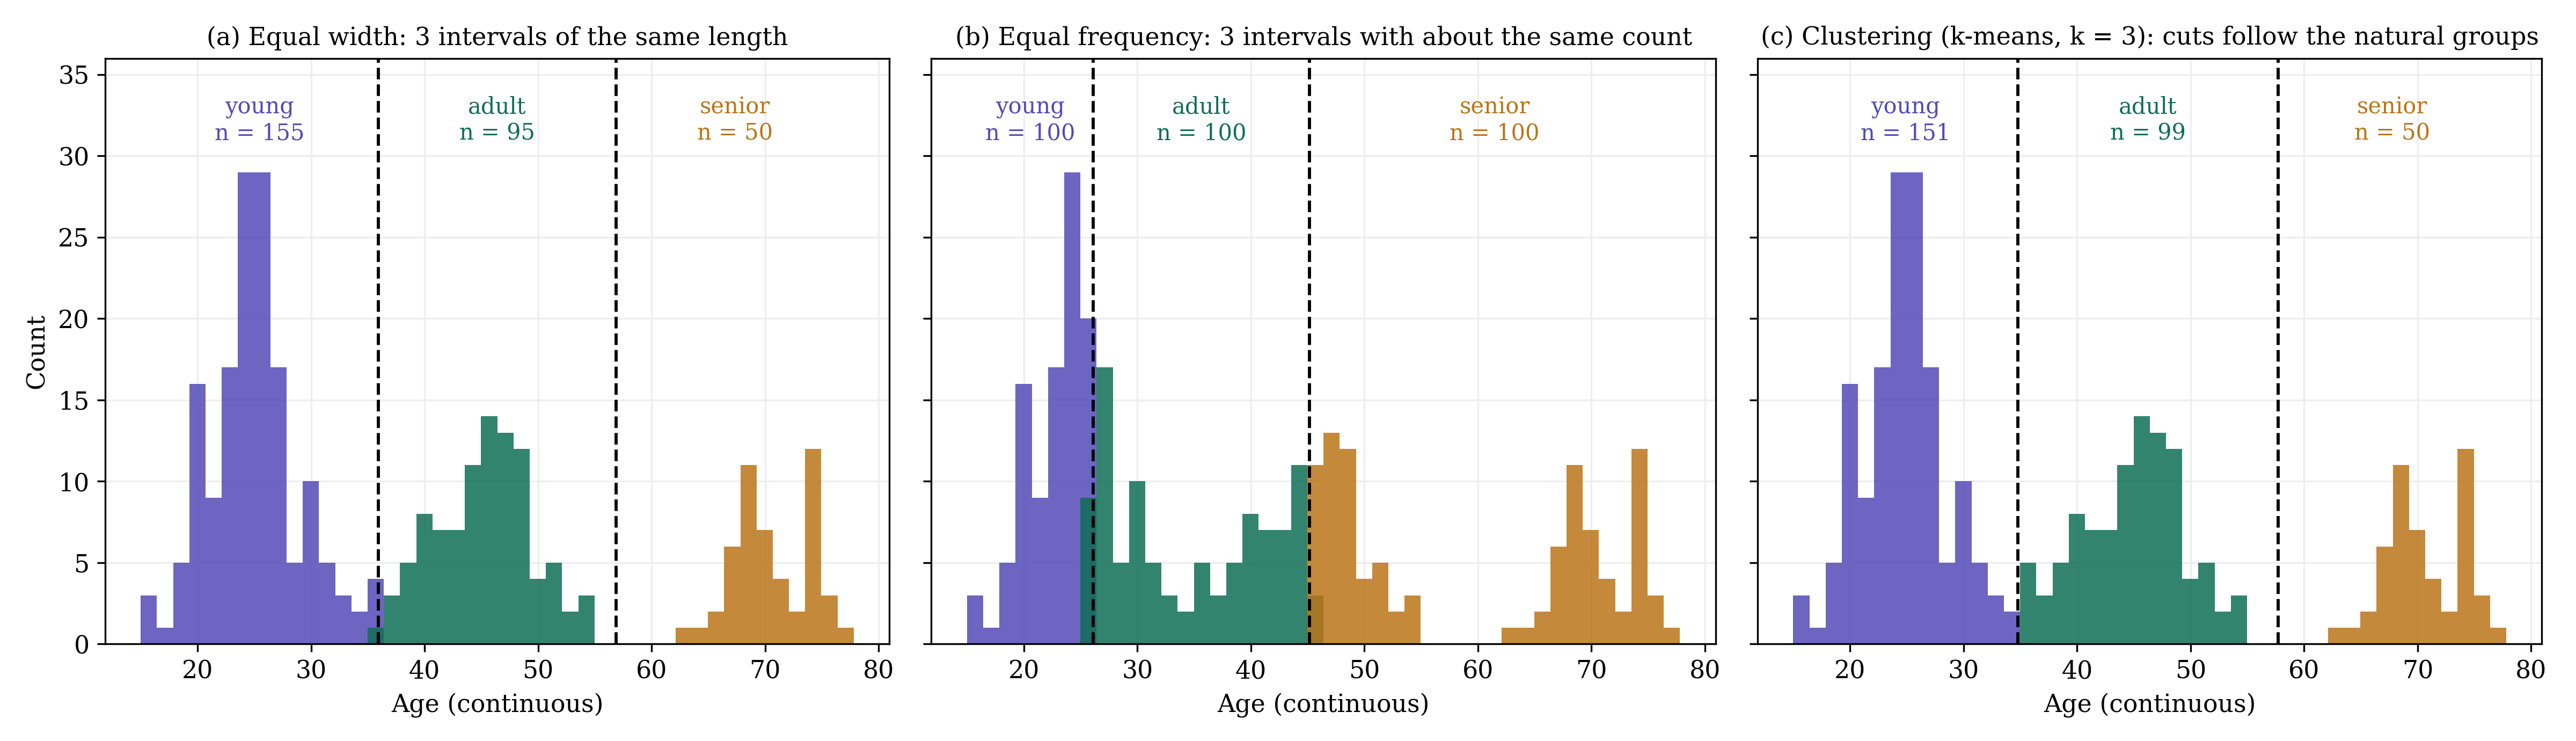
\includegraphics[width=0.8\textwidth]{images/chapter_3/discretization.png}
    \caption{Discretization of a continuous attribute (age) into 3 bins with three unsupervised techniques. The dashed lines are the cut points; each colour is one category.}
\end{figure}

\begin{itemize}
    \item \textbf{Equal width:} $N$ intervals of the same length. Simple, but some bins may contain very few points, and it is sensitive to outliers.
    \item \textbf{Equal frequency:} $N$ intervals with approximately the same number of points. Each bin is well populated, but similar values may be split into different bins.
    \item \textbf{Clustering:} the cuts are placed between natural groups of values found by a clustering algorithm (e.g.\ k-means).
\end{itemize}

\subsection{Data Binarization}
Binarization maps an attribute into one or more \textbf{binary} variables (0/1).
\begin{itemize}
    \item \textbf{Continuous attribute:} first discretize it into categories, then apply one of the techniques for categorical attributes below. Example: age $\rightarrow$ \{young, adult, senior\} $\rightarrow$ binary vector.
    \item \textbf{Categorical attribute:} map it to a set of binary attributes, for instance via \emph{one-hot encoding}.
\end{itemize}
Why not simply map the categories to integers (San Francisco $=1$, New York $=2$, Seattle $=3$)? Because the model would assume an order and a distance that do not exist (Seattle would be ``greater'' than San Francisco, and New York would be ``halfway'' between them). The following encodings avoid this problem. In all of them, a categorical variable with $k$ categories is represented by a group of bits.

\begin{itemize}
    \item \textbf{One-Hot Encoding:} one bit per category ($k$ bits). Since an object belongs to only one category, exactly one bit is set to 1. The result is a \emph{sparse} matrix (mostly zeros).
    \item \textbf{Dummy Coding:} only $k-1$ bits. One category is chosen as \emph{reference} and is encoded with all zeros; the other categories are encoded as in one-hot.
    \item \textbf{Effect Coding:} like dummy coding, but the reference category is encoded with all $-1$s instead of all $0$s.
\end{itemize}

\begin{center}
    \small
    \renewcommand{\arraystretch}{1.3}
    \begin{tabular}{|l|c|c|c||c|c||c|c|}
    \hline
     & \multicolumn{3}{c||}{\textbf{One-Hot}} & \multicolumn{2}{c||}{\textbf{Dummy}} & \multicolumn{2}{c|}{\textbf{Effect}} \\
    \hline
     & $e_1$ & $e_2$ & $e_3$ & $e_1$ & $e_2$ & $e_1$ & $e_2$ \\
    \hline
    San Francisco & 1 & 0 & 0 & 1 & 0 & 1 & 0 \\
    \hline
    New York & 0 & 1 & 0 & 0 & 1 & 0 & 1 \\
    \hline
    Seattle (reference) & 0 & 0 & 1 & 0 & 0 & $-1$ & $-1$ \\
    \hline
    \end{tabular}
\end{center}

\paragraph{Why $k-1$ bits are enough.} One-hot encoding uses $k$ bits, i.e.\ it has $k$ degrees of freedom, but the variable only needs $k-1$. In the example, if $e_1=0$ and $e_2=0$, the city \emph{must} be Seattle, so $e_3$ adds no information: it can always be computed as $e_3 = 1-e_1-e_2$. This redundancy is a problem for linear models, because the model can no longer find a unique set of coefficients (many combinations give exactly the same predictions). Dummy and effect coding remove the extra bit.

\paragraph{Pros and cons.} When these encodings are used in a linear model, they also change how the coefficients are interpreted:

\begin{center}
    \small
    \renewcommand{\arraystretch}{1.3}
    \begin{tabular}{|l|p{4.6cm}|p{4.6cm}|}
        \hline
        & \textbf{PROS} & \textbf{CONS} \\
        \hline
        \textbf{One-Hot} & each feature clearly corresponds to one category; missing data can be encoded as the all-zeros vector; the intercept of a linear model represents the overall mean of the target variable & redundant ($k$ bits for $k-1$ degrees of freedom): the linear model has no unique solution \\
        \hline
        \textbf{Dummy} & not redundant ($k-1$ bits): the solution is unique; the intercept is the mean of the target for the reference category & cannot easily handle missing data, since the all-zeros vector is already used by the reference category \\
        \hline
        \textbf{Effect} & not redundant; the reference category uses a different code ($-1$s), so the all-zeros vector is free for missing data; the intercept represents the overall mean & the vector of all $-1$s is dense (not sparse), which is expensive for both storage and computation \\
        \hline
    \end{tabular}
\end{center}

\subsection{Attribute Transformation}
An attribute transformation is a function that maps \emph{all} the values of an attribute to a new set of values, so that each old value corresponds to exactly one new value. Examples: $x \rightarrow \log x$ (to compress very skewed values), $x \rightarrow |x|$, and normalization.

\textbf{Normalization} is used to make attributes with different scales comparable. If age ranges in $[20,70]$ and income in $[20\,000,100\,000]$, any distance between two people would depend almost only on income, simply because its numbers are bigger. After normalization all attributes contribute in a comparable way. The two most common techniques are:

\begin{figure}[htbp]
    \centering
    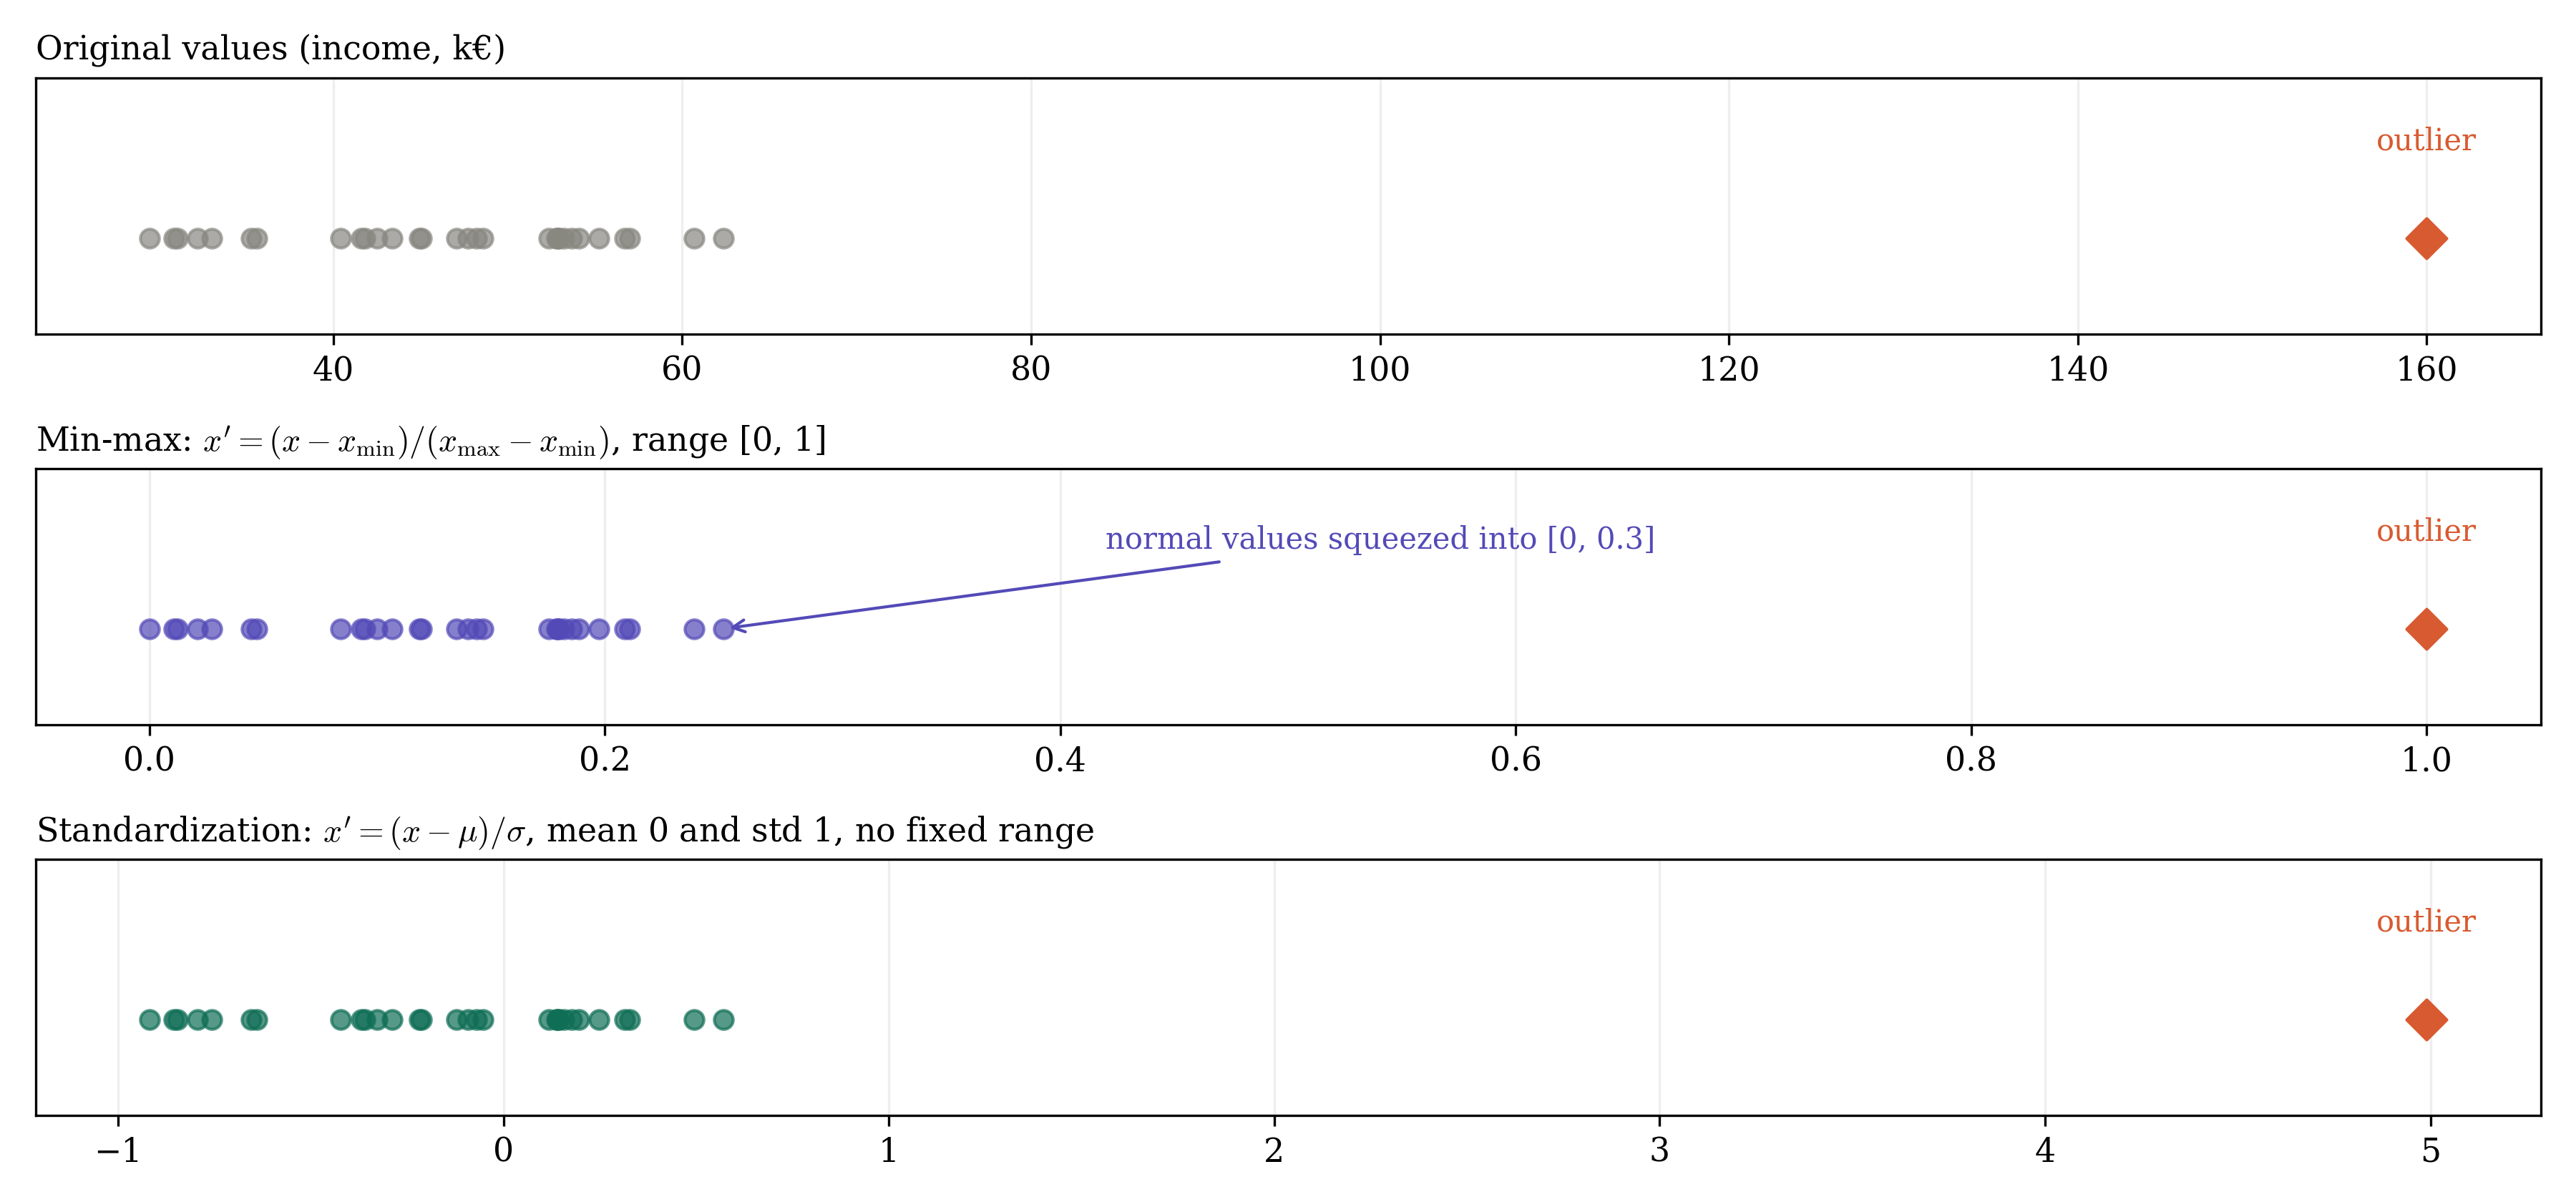
\includegraphics[width=0.9\textwidth]{images/chapter_3/normalization.png}
    \caption{Effect of normalization on data with an outlier. Min-max normalization maps the outlier to 1 and compresses all the normal values close to 0; standardization centres the data around 0 without a fixed range.}
\end{figure}

\begin{itemize}
    \item \textbf{Min-Max Normalization:} rescales the values linearly into the range $[0,1]$: the minimum becomes $0$ and the maximum becomes $1$.
    \[
        x'=\frac{x-x_{\min}}{x_{\max}-x_{\min}}
    \]
    It retains the shape of the distribution, but it is \textbf{sensitive to outliers}: a single extreme value becomes the maximum and squeezes all the other values into a small part of the range (Figure~\ref{fig:normalization}). Example: with $x_{\min}=20$ and $x_{\max}=70$, the value $x=45$ becomes $x'=25/50=0.5$.
    \item \textbf{Standardization (z-score):} subtracts the mean $\mu$ and divides by the standard deviation $\sigma$, so that the new values have zero mean and unit standard deviation.
    \[
        x'=\frac{x-\mu}{\sigma}
    \]
    The new value tells \emph{how many standard deviations} $x$ is from the mean. It is not bounded to a fixed range, and outliers remain clearly visible as large values. Example: with $\mu=50$ and $\sigma=10$, the value $x=70$ becomes $x'=2$.
\end{itemize}


\noindent\textbf{Note:} the parameters ($x_{\min}$, $x_{\max}$, $\mu$, $\sigma$) must be computed on the training data only, and then applied unchanged to the test data.

\subsection{Data Preparation for Document Data}
Most algorithms cannot process raw text directly: they need numbers. For this reason a document is usually represented as a set of features. \textbf{Document PreProcessing} is the activity that generates a structured representation of documents, and it includes five sequential steps:
\begin{enumerate}
    \item \textbf{Document Splitting:} depending on the goal of the analysis, documents are split into sentences or paragraphs, or analysed in their entire content.
    \item \textbf{Tokenization:} breaking the text into units called \emph{tokens}, typically words, for instance by separating words at spaces and identifying sentence boundaries based on punctuation.
    \item \textbf{Case Normalization:} converting every token to lower-case (or upper-case), so that ``The'' and ``the'' are treated as the same word.
    \item \textbf{Stopword Elimination:} removing \emph{stopwords}, the most common words of a language (articles, prepositions, auxiliary verbs, \dots), which appear everywhere and carry little meaning.
    \item \textbf{Stemming:} reducing each word to its root (\emph{stem}), so that different forms of the same word are counted together: ``running'', ``runs'' $\rightarrow$ ``run''; ``cats'' $\rightarrow$ ``cat''.
\end{enumerate}

The following example shows how one sentence changes at each step:

\begin{center}
    \small
    \renewcommand{\arraystretch}{1.3}
    \begin{tabular}{|l|p{7.7cm}|}
    \hline
    \textbf{Step} & \textbf{Result} \\
    \hline
    Original text & \texttt{The cats are running in the garden. The dog runs and the dog barks.} \\
    \hline
    1. Splitting & S1: \texttt{The cats are running in the garden.} \newline S2: \texttt{The dog runs and the dog barks.} \\
    \hline
    2. Tokenization (S1) & \texttt{[The, cats, are, running, in, the, garden]} \\
    \hline
    3. Case normalization & \texttt{[the, cats, are, running, in, the, garden]} \\
    \hline
    4. Stopword elimination & \texttt{[cats, running, garden]} \\
    \hline
    5. Stemming & \texttt{[cat, run, garden]} \\
    \hline
    \end{tabular}
\end{center}

\paragraph{Term vectors (bag of words).} After preprocessing, each document is represented as a \textbf{term vector}: each distinct term is an attribute, and the value of the attribute is the number of times the term occurs in the document. The order of the words is ignored. Putting all the vectors together gives the \textbf{document-term matrix}. Example with three short documents:
\begin{itemize}
    \item $D_1$: ``The cats are running in the garden'' $\rightarrow$ \{cat, run, garden\}
    \item $D_2$: ``The dog runs and the dog barks'' $\rightarrow$ \{dog, run, dog, bark\}
    \item $D_3$: ``A dog and a cat in the garden'' $\rightarrow$ \{dog, cat, garden\}
\end{itemize}

\begin{center}
    \small
    \renewcommand{\arraystretch}{1.3}
    \begin{tabular}{|l|c|c|c|c|c|}
    \hline
     & \textbf{bark} & \textbf{cat} & \textbf{dog} & \textbf{garden} & \textbf{run} \\
    \hline
    $D_1$ & 0 & 1 & 0 & 1 & 1 \\
    \hline
    $D_2$ & 1 & 0 & 2 & 0 & 1 \\
    \hline
    $D_3$ & 0 & 1 & 1 & 1 & 0 \\
    \hline
    \end{tabular}
\end{center}

\paragraph{Weighting schemes.} The value of each term can be computed in different ways:
\begin{itemize}
    \item \textbf{Binary:} $1$ if the term appears in the document, $0$ otherwise.
    \item \textbf{Term Frequency (TF):} the number of occurrences of the term in the document (as in the table above).
    \item \textbf{TF-IDF:} the term frequency multiplied by a factor that rewards rare terms and penalises terms that appear in many documents:
    \[
        \text{tf-idf}(t,d)=\text{tf}(t,d)\cdot\log\frac{N}{\text{df}(t)}
    \]
    where $N$ is the number of documents and $\text{df}(t)$ is the number of documents containing term $t$. A term that appears in every document gets weight $\log 1 = 0$, because it does not help to distinguish documents. In the example ($N=3$, natural logarithm), ``bark'' appears only in $D_2$, so its weight is $1\cdot\log 3\approx1.10$, while ``dog'' appears in two documents and gets $2\cdot\log 1.5\approx0.81$ in $D_2$, even though it occurs twice.
\end{itemize}


\section{A prova di coglione}

\subsection*{Attributi e dati}
Un \textbf{attributo} è una caratteristica (es.\ l'altezza), il \textbf{valore} è il modo in cui la misuriamo (metri o piedi). Lo stesso attributo può avere valori diversi, e attributi diversi possono avere gli stessi valori (ID ed età sono entrambi interi).

\begin{center}
\small
\begin{tabular}{@{}lll@{}}
\toprule
\textbf{Tipo} & \textbf{Cosa posso fare} & \textbf{Esempio} \\
\midrule
Nominale & solo dire se sono uguali ($=$) & colore degli occhi, ID \\
Ordinale & uguali e ordinarli ($<,=,>$) & voti, taglie S/M/L \\
Discreto & pochi valori, spesso interi (binario = caso speciale) & conteggi, 0/1 \\
Continuo & numeri reali & altezza, temperatura \\
\bottomrule
\end{tabular}
\end{center}

\noindent I dati possono essere \textbf{tabelle}, \textbf{documenti} (testo), \textbf{grafi} (il Web) o \textbf{dati ordinati} (serie temporali, genoma).

\paragraph*{Qualità.} Ogni dataset ha dei difetti:
\begin{itemize}
    \item \textbf{Rumore}: valori alterati a caso (es.\ errori di misura). \textbf{Outlier}: oggetti molto diversi dagli altri; a volte disturbano, a volte sono proprio ciò che cerchiamo.
    \item \textbf{Valori mancanti}: si eliminano, si stimano o si ignorano.
    \item \textbf{Duplicati}: tipici quando si uniscono più fonti; vanno ripuliti.
\end{itemize}

\subsection*{Similarità e distanza}
La \textbf{dissimilarità} $d$ vale $0$ se due oggetti sono identici e cresce quanto più sono diversi. La \textbf{similarità} $s$ fa l'opposto: di solito sta in $[0,1]$ e vale $1$ per oggetti identici.

\paragraph*{Un solo attributo.}
\begin{itemize}
    \item \textbf{Nominale}: o uguali ($d=0$) o diversi ($d=1$), senza vie di mezzo.
    \item \textbf{Ordinale}: si numerano i valori da $0$ a $n-1$ e $d=\frac{|x-y|}{n-1}$, $s=1-d$. Con \{poor, fair, good, excellent\}: $d(\text{poor},\text{good})=2/3$. Si assume che i ``gradini'' siano tutti uguali.
    \item \textbf{Numerico}: $d=|x-y|$. Per la similarità: $s=-d$, $s=\frac{1}{1+d}$, $s=e^{-d}$ oppure min-max. Con $d=2$: $-2$, $0.33$, $0.14$.
\end{itemize}

\paragraph*{Più attributi: Minkowski.} Ogni oggetto è un punto in $n$ dimensioni e
\[
d(\mathbf{x},\mathbf{y})=\Big(\sum_{k=1}^{n}|x_k-y_k|^r\Big)^{1/r}
\]
Il parametro $r$ (scelto da noi, non è $n$) decide come combinare le differenze:
$r=1$ \textbf{Manhattan} (somma delle differenze, come camminare tra isolati),
$r=2$ \textbf{Euclidea} (linea retta),
$r\to\infty$ \textbf{Chebyshev} (solo la differenza più grande).
Esempio: $\mathbf{x}=(1,1)$, $\mathbf{y}=(4,5)$, differenze $3$ e $4$ $\Rightarrow$ $L_1=7$, $L_2=5$, $L_\infty=4$.
Se gli attributi hanno scale diverse (euro vs anni) vince quello con i numeri più grandi: prima si \textbf{standardizza}.

\paragraph*{Quando una distanza è una metrica.} Deve rispettare: $d(x,x)=0$; $d(x,y)>0$ se $x\neq y$; $d(x,y)=d(y,x)$; e la \textbf{disuguaglianza triangolare} $d(x,z)\le d(x,y)+d(y,z)$ (la strada diretta non è mai più lunga di una deviazione). Minkowski è una metrica solo per $r\ge1$: con $r=0.5$, $x=(0,0)$, $y=(1,0)$, $z=(1,1)$ si ottiene $d(x,z)=4 > 1+1$.

\paragraph*{Mahalanobis.} Idea: \emph{una differenza pesa tanto quanto è insolita}.
\[
d(\mathbf{x},\mathbf{y})=\sqrt{(\mathbf{x}-\mathbf{y})^\top S^{-1}(\mathbf{x}-\mathbf{y})}
\]
dove $S$ è la matrice di covarianza. Dove i dati variano molto, una differenza conta poco; dove variano poco, conta molto. Tiene conto anche delle correlazioni, così le informazioni ripetute non contano due volte. Non dipende dalle unità di misura. Se $S=I$ torna la distanza euclidea; se $S$ è diagonale equivale all'euclidea su dati standardizzati.
Esempio con varianze $4$ e $1$: la differenza $(2,0)$ dà $d=1$, la differenza $(0,2)$ dà $d=2$. Stessa distanza euclidea, ma la seconda è più ``strana''.

\subsection*{Preprocessing}
I dati reali sono sporchi, enormi, con troppi attributi o non numerici. Il preprocessing li rende puliti, compatti e utilizzabili.

\paragraph*{Aggregazione.} Più valori diventano uno solo (somma o media): giorni $\to$ mesi, città $\to$ regioni. Si ottengono meno dati, una visione d'insieme e valori più stabili (nella media le oscillazioni si compensano). Si perde però il dettaglio.

\paragraph*{Riduzione.} Un dataset più piccolo che dà quasi gli stessi risultati: \textbf{meno righe} (campionamento), \textbf{meno colonne} (selezione delle feature), \textbf{meno valori} (discretizzazione).

\paragraph*{Campionamento.} Si analizza solo una parte dei dati, che deve essere \textbf{rappresentativa} (stesse medie, stesse proporzioni delle classi).
\textbf{Casuale semplice}: tutti hanno la stessa probabilità, ma una classe rara può sparire per caso.
\textbf{Stratificato}: si campiona da ogni gruppo in proporzione alla sua dimensione, così nessuna classe si perde.

\paragraph*{Maledizione della dimensionalità.} Con tante dimensioni lo spazio diventa enorme e i dati \textbf{vuoti e sparsi}. Per prendere il 10\% dei dati in un cubo serve un lato di $0.1$ in 1D, ma di $0.79$ in 10D: il ``vicino'' non è più vicino. Inoltre tutti i punti diventano quasi equidistanti, quindi distanza e densità (base di clustering e outlier detection) perdono senso.

\paragraph*{Selezione delle feature.} Si tolgono feature \textbf{ridondanti} (prezzo con e senza IVA) e \textbf{irrilevanti} (la matricola per prevedere il voto). Metodi:
\begin{itemize}
    \item \textbf{RFE}: addestro il modello, elimino la feature meno importante, riaddestro, ripeto fino al numero voluto. Si riaddestra ogni volta perché le importanze cambiano; per questo è lento con molte feature.
    \item \textbf{Modelli interpretabili}: alberi di decisione e regressione lineare dicono già quanto pesa ogni feature.
    \item \textbf{PCA/SVD}: non scelgono feature, ne \emph{creano} di nuove combinando le originali; poche componenti contengono quasi tutta l'informazione.
\end{itemize}

\paragraph*{Feature engineering.} Trasformare i dati grezzi nella forma più utile al modello: spesso conta più dell'algoritmo. Dati strutturati $\to$ normalizzazione, discretizzazione, binarizzazione; testo, immagini, segnali $\to$ tokenizzazione, Fourier, descrittori.

\paragraph*{Trasformazione.} Cambiare rappresentazione per far emergere l'informazione. Esempio: la \textbf{trasformata di Fourier} trasforma un segnale di 1000 valori nel tempo in due soli picchi di frequenza.

\paragraph*{Discretizzazione.} Da continuo a categorie ordinate: età $\to$ \{giovane, adulto, anziano\}. Più facile da interpretare, ma si perde dettaglio.
\textbf{Equal width}: intervalli della stessa ampiezza (semplice, sensibile agli outlier).
\textbf{Equal frequency}: stesso numero di punti per intervallo.
\textbf{Clustering}: tagli tra i gruppi naturali (es.\ k-means).

\paragraph*{Binarizzazione.} Le categorie diventano bit. Non si usano numeri (SF=1, NY=2, Seattle=3) perché inventerebbero un ordine che non esiste.
\begin{center}
    \small
    \begin{tabular}{@{}l|ccc|cc|cc@{}}
        \toprule
        & \multicolumn{3}{c|}{\textbf{One-hot}} & \multicolumn{2}{c|}{\textbf{Dummy}} & \multicolumn{2}{c}{\textbf{Effect}} \\
        \midrule
        San Francisco & 1 & 0 & 0 & 1 & 0 & 1 & 0 \\
        New York      & 0 & 1 & 0 & 0 & 1 & 0 & 1 \\
        Seattle       & 0 & 0 & 1 & 0 & 0 & $-1$ & $-1$ \\
        \bottomrule
    \end{tabular}
\end{center}

Il \textbf{one-hot} usa $k$ bit, ma uno è inutile: se i primi due sono $0$, la città è per forza Seattle. Questo confonde i modelli lineari (nessuna soluzione unica). \textbf{Dummy} ed \textbf{effect} usano $k-1$ bit e risolvono il problema.
In breve: \emph{one-hot} è chiaro e gestisce i mancanti (vettore nullo) ma è ridondante; \emph{dummy} non è ridondante ma il vettore nullo è già occupato; \emph{effect} risolve entrambi, ma i $-1$ rendono i dati densi e costosi.

\paragraph*{Normalizzazione.} Rende confrontabili scale diverse (età 20--70 vs reddito 20\,000--100\,000).
\begin{itemize}
    \item \textbf{Min-max}: $x'=\frac{x-x_{\min}}{x_{\max}-x_{\min}}\in[0,1]$. Un outlier però schiaccia tutti gli altri valori verso $0$.
    \item \textbf{Z-score}: $x'=\frac{x-\mu}{\sigma}$, cioè ``a quante deviazioni standard dalla media''. Gli outlier restano visibili.
\end{itemize}
Media, min e max si calcolano \textbf{solo sul training set}.

\paragraph*{Documenti.} Il testo va trasformato in numeri in cinque passi:
\begin{center}
    \small
    \texttt{The cats are running in the garden.}
    $\xrightarrow{\text{token}}$ \texttt{[The, cats, are, running, in, the, garden]}\\[2pt]
    $\xrightarrow{\text{minuscolo}}$ \texttt{[the, cats, \dots]}
    $\xrightarrow{\text{via stopword}}$ \texttt{[cats, running, garden]}
    $\xrightarrow{\text{stemming}}$ \texttt{[cat, run, garden]}
    \end{center}
    (il primo passo, lo \emph{splitting}, divide il testo in frasi o paragrafi). Poi ogni documento diventa un vettore che conta le parole (\textbf{bag of words}), ignorandone l'ordine:
    \begin{center}
    \small
    \begin{tabular}{@{}lccccc@{}}
    \toprule
    & bark & cat & dog & garden & run \\
    \midrule
    $D_1$: The cats are running in the garden & 0 & 1 & 0 & 1 & 1 \\
    $D_2$: The dog runs and the dog barks & 1 & 0 & 2 & 0 & 1 \\
    $D_3$: A dog and a cat in the garden & 0 & 1 & 1 & 1 & 0 \\
    \bottomrule
    \end{tabular}
\end{center}

I pesi possono essere \textbf{binari} (c'è o no), \textbf{TF} (quante volte) o \textbf{TF-IDF}, che premia le parole rare:
\[
\text{tf-idf}(t,d)=\text{tf}(t,d)\cdot\log\frac{N}{\text{df}(t)}
\]
Una parola presente in tutti i documenti pesa $0$, perché non aiuta a distinguerli. Nell'esempio ``bark'' vale $\log 3\approx1.10$, mentre ``dog'' vale solo $0.81$ pur comparendo due volte.
%\chapter{Dimensionality Reduction}

The \textbf{curse of dimensionality} makes multivariate data hard both to \emph{visualize} and to \emph{extract useful information from}. Dimensionality Reduction tackles this problem by ``\emph{solving problems by changing the viewpoint}'': it automatically finds good features by learning a hypothesis map that reads the representation of a data point and transforms it into a smaller set of features. The aim is to obtain a \textbf{compressed representation} of the data. Note that, in this sense, feature engineering also means \textbf{feature reduction}.

Reducing the number of features is good practice because it allows to:

\begin{itemize}
    \item Capture the important information in a dataset more efficiently than the original attributes.
    \item Visualize data more easily.
    \item Reduce \underline{overfitting}, improving the generalization of models.
    \item Avoid the curse of dimensionality.
    \item Reduce the time and memory required by algorithms.
    \item Eliminate irrelevant features and reduce noise.
\end{itemize}

The main techniques are: Singular Value Decomposition (SVD), Principal Component Analysis (PCA), Linear Discriminant Analysis (LDA) and non-linear techniques (e.g.\ Kernel PCA, t-SNE).

\begin{figure}[h]
    \centering
    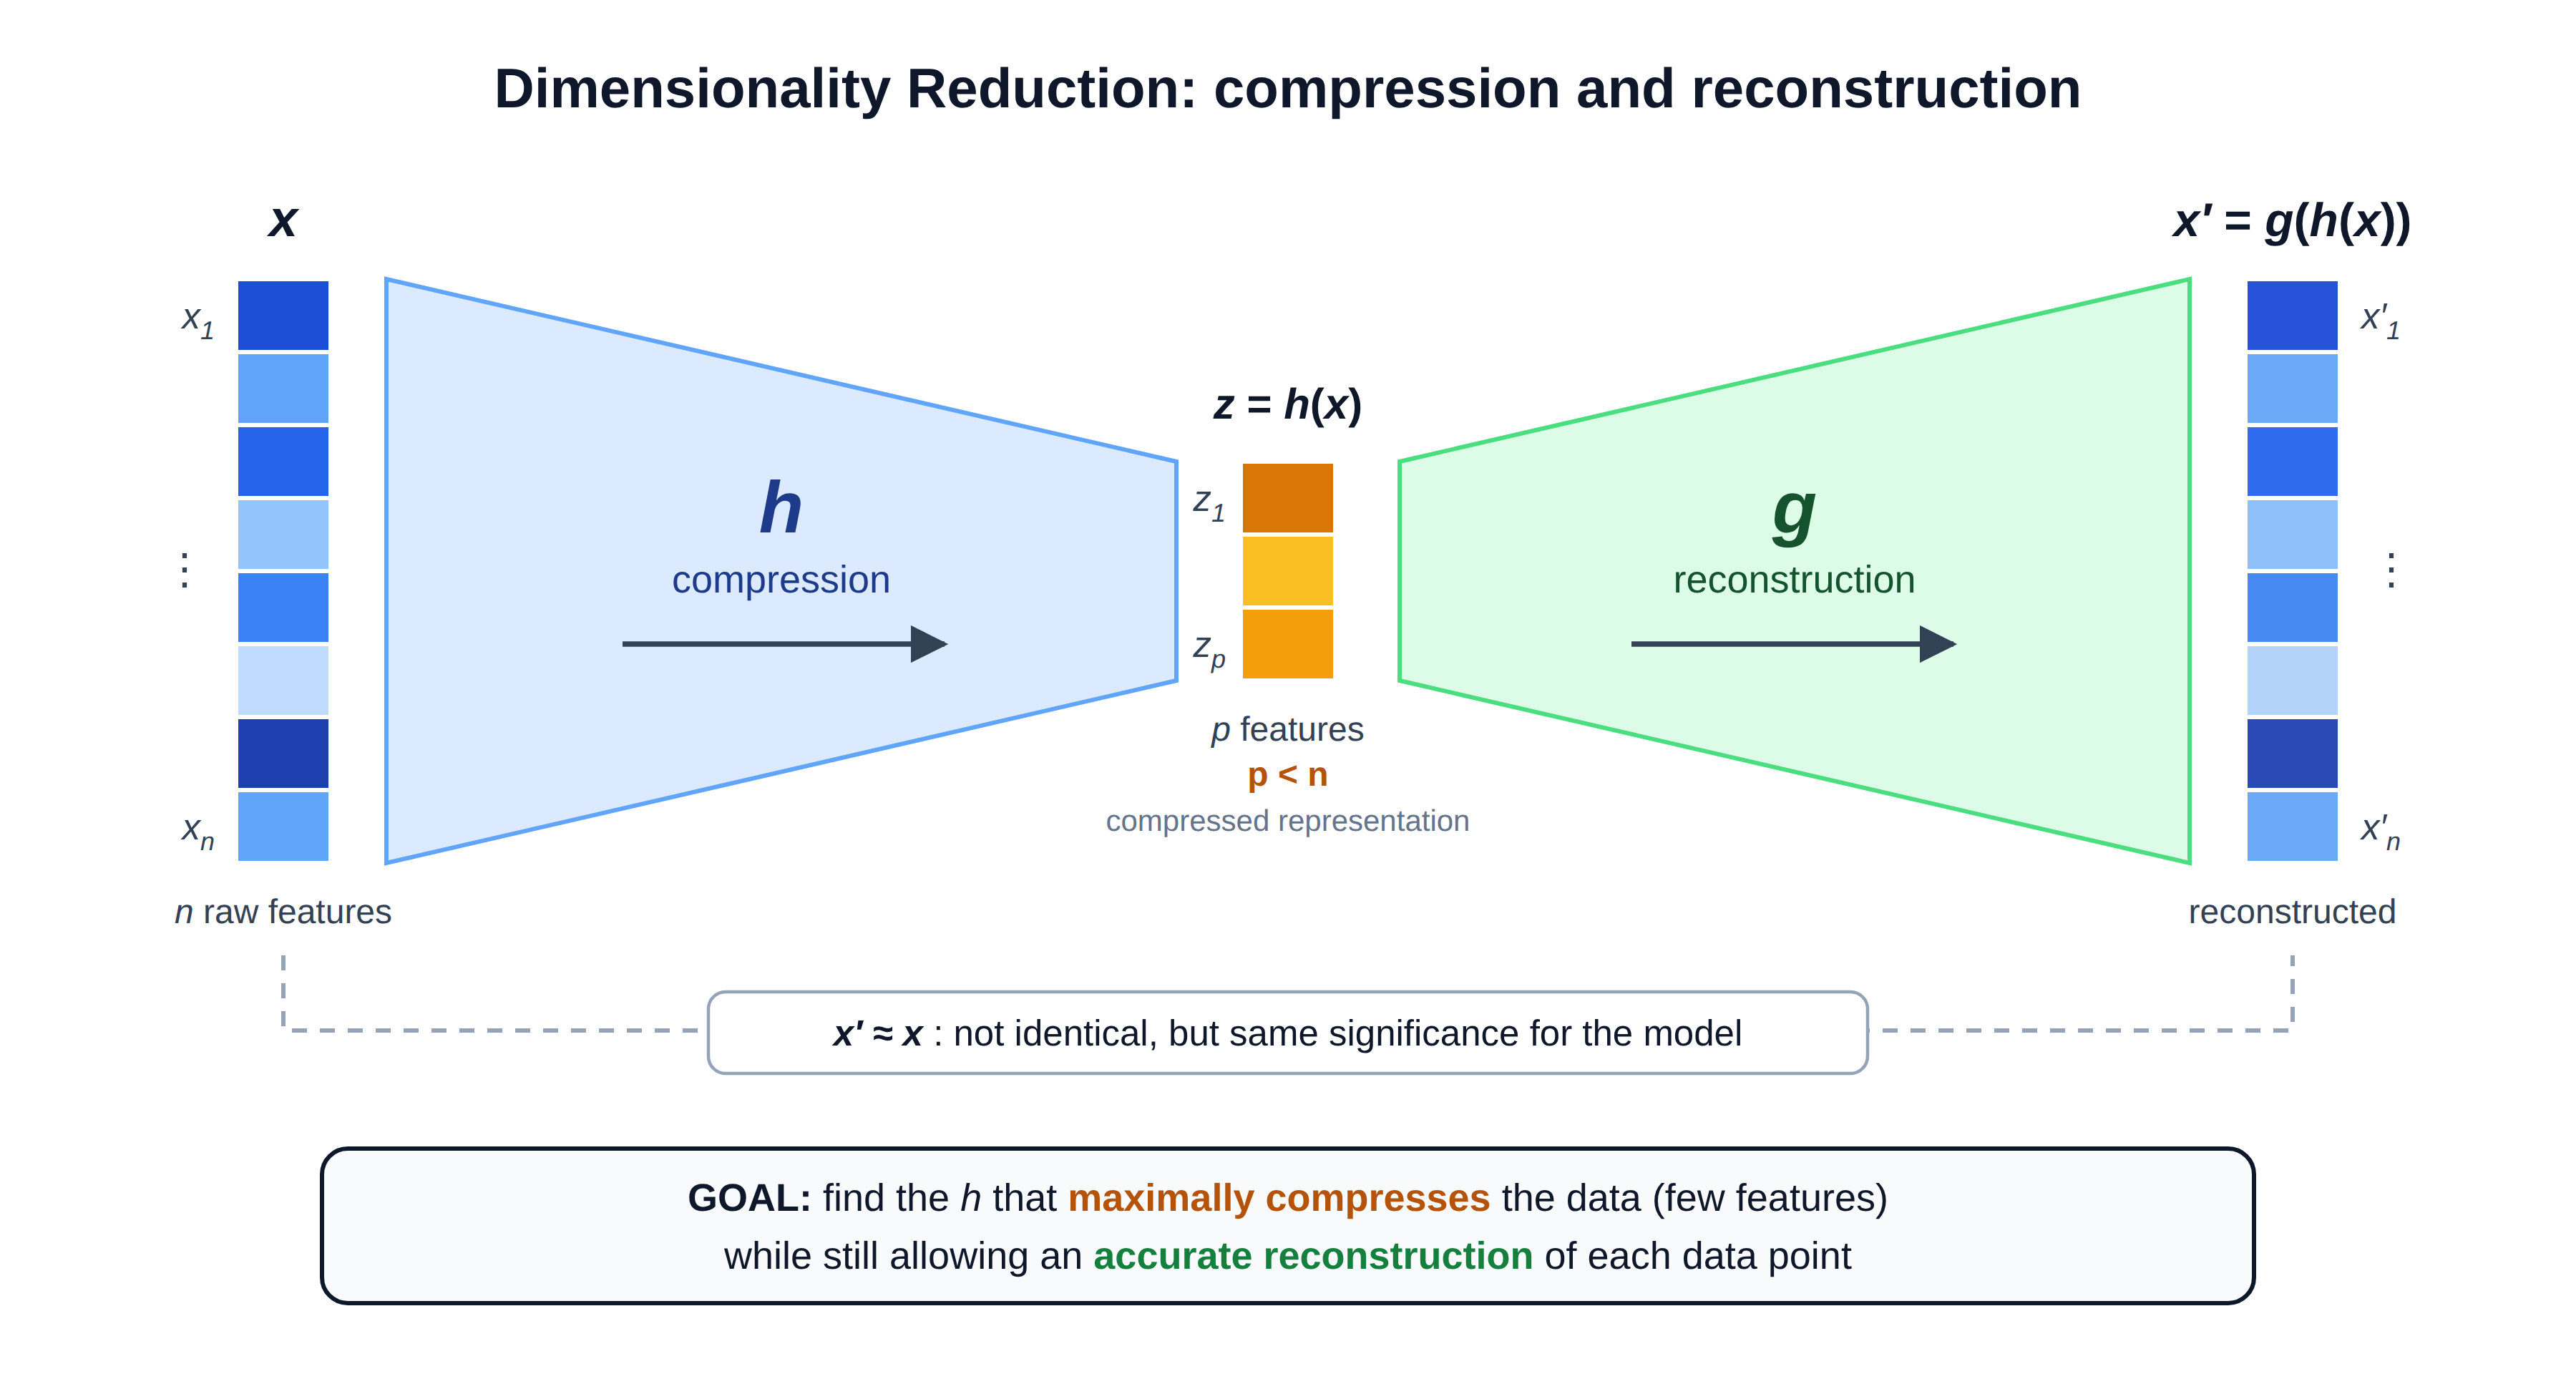
\includegraphics[width=0.6\textwidth]{images/chapter_4/dr_compression_reconstruction.png}
    \caption{Compression map $h$ and reconstruction map $g$}
\end{figure}

Every Dimensionality Reduction process is built around two maps:

\begin{itemize}
    \item \textbf{Compression}: a map $h$ that goes from $n$ raw features to $p$ features ($p < n$), producing the compressed representation $z = h(x)$.
    \item \textbf{Reconstruction}: a map $g$ that recovers the original values from the compressed ones, $x' = g(h(x))$. The reconstructed $x'$ is not exactly equal to $x$, but very similar, i.e.\ it carries the same significance with respect to the model.
    \item \textbf{Goal}: find the $h$ that \emph{maximally compresses} the raw data while still allowing an \emph{accurate reconstruction} of each data point from a small number of features.
\end{itemize}

\section{PCA: Principal Component Analysis}
PCA was introduced by Pearson and Hotelling to describe the variation in a set of multivariate data in terms of a set of \textbf{uncorrelated} variables. We start from a data matrix $X$ ($m \times n$): each \emph{row} is an observation (a data point), each \emph{column} is one of the $n$ correlated variables $x_1, x_2, \dots, x_n$. PCA transforms them into $p \le n$ new variables $x'_i$ that are \textbf{uncorrelated}. To do so it builds a \textbf{new basis} (a new set of axes) in which the \textbf{first axis carries the maximum information} about the data. For PCA, information means \textbf{variance}: a direction along which the data are very spread out tells us a lot, while a direction along which all points are almost equal tells us almost nothing.

PCA is useful when there is \textbf{redundancy} in the variables, i.e.\ when the \textbf{data do not span the whole $n$-dimensional space}. Redundancy means that some variables are \textbf{correlated}: if $x_2$ almost always grows with $x_1$, the two variables largely carry the same information. Because of it, the observed variables can be summarized by a \textbf{smaller number of principal components} that still account for \textbf{most of the variance}.

\begin{figure}[h]
    \centering
    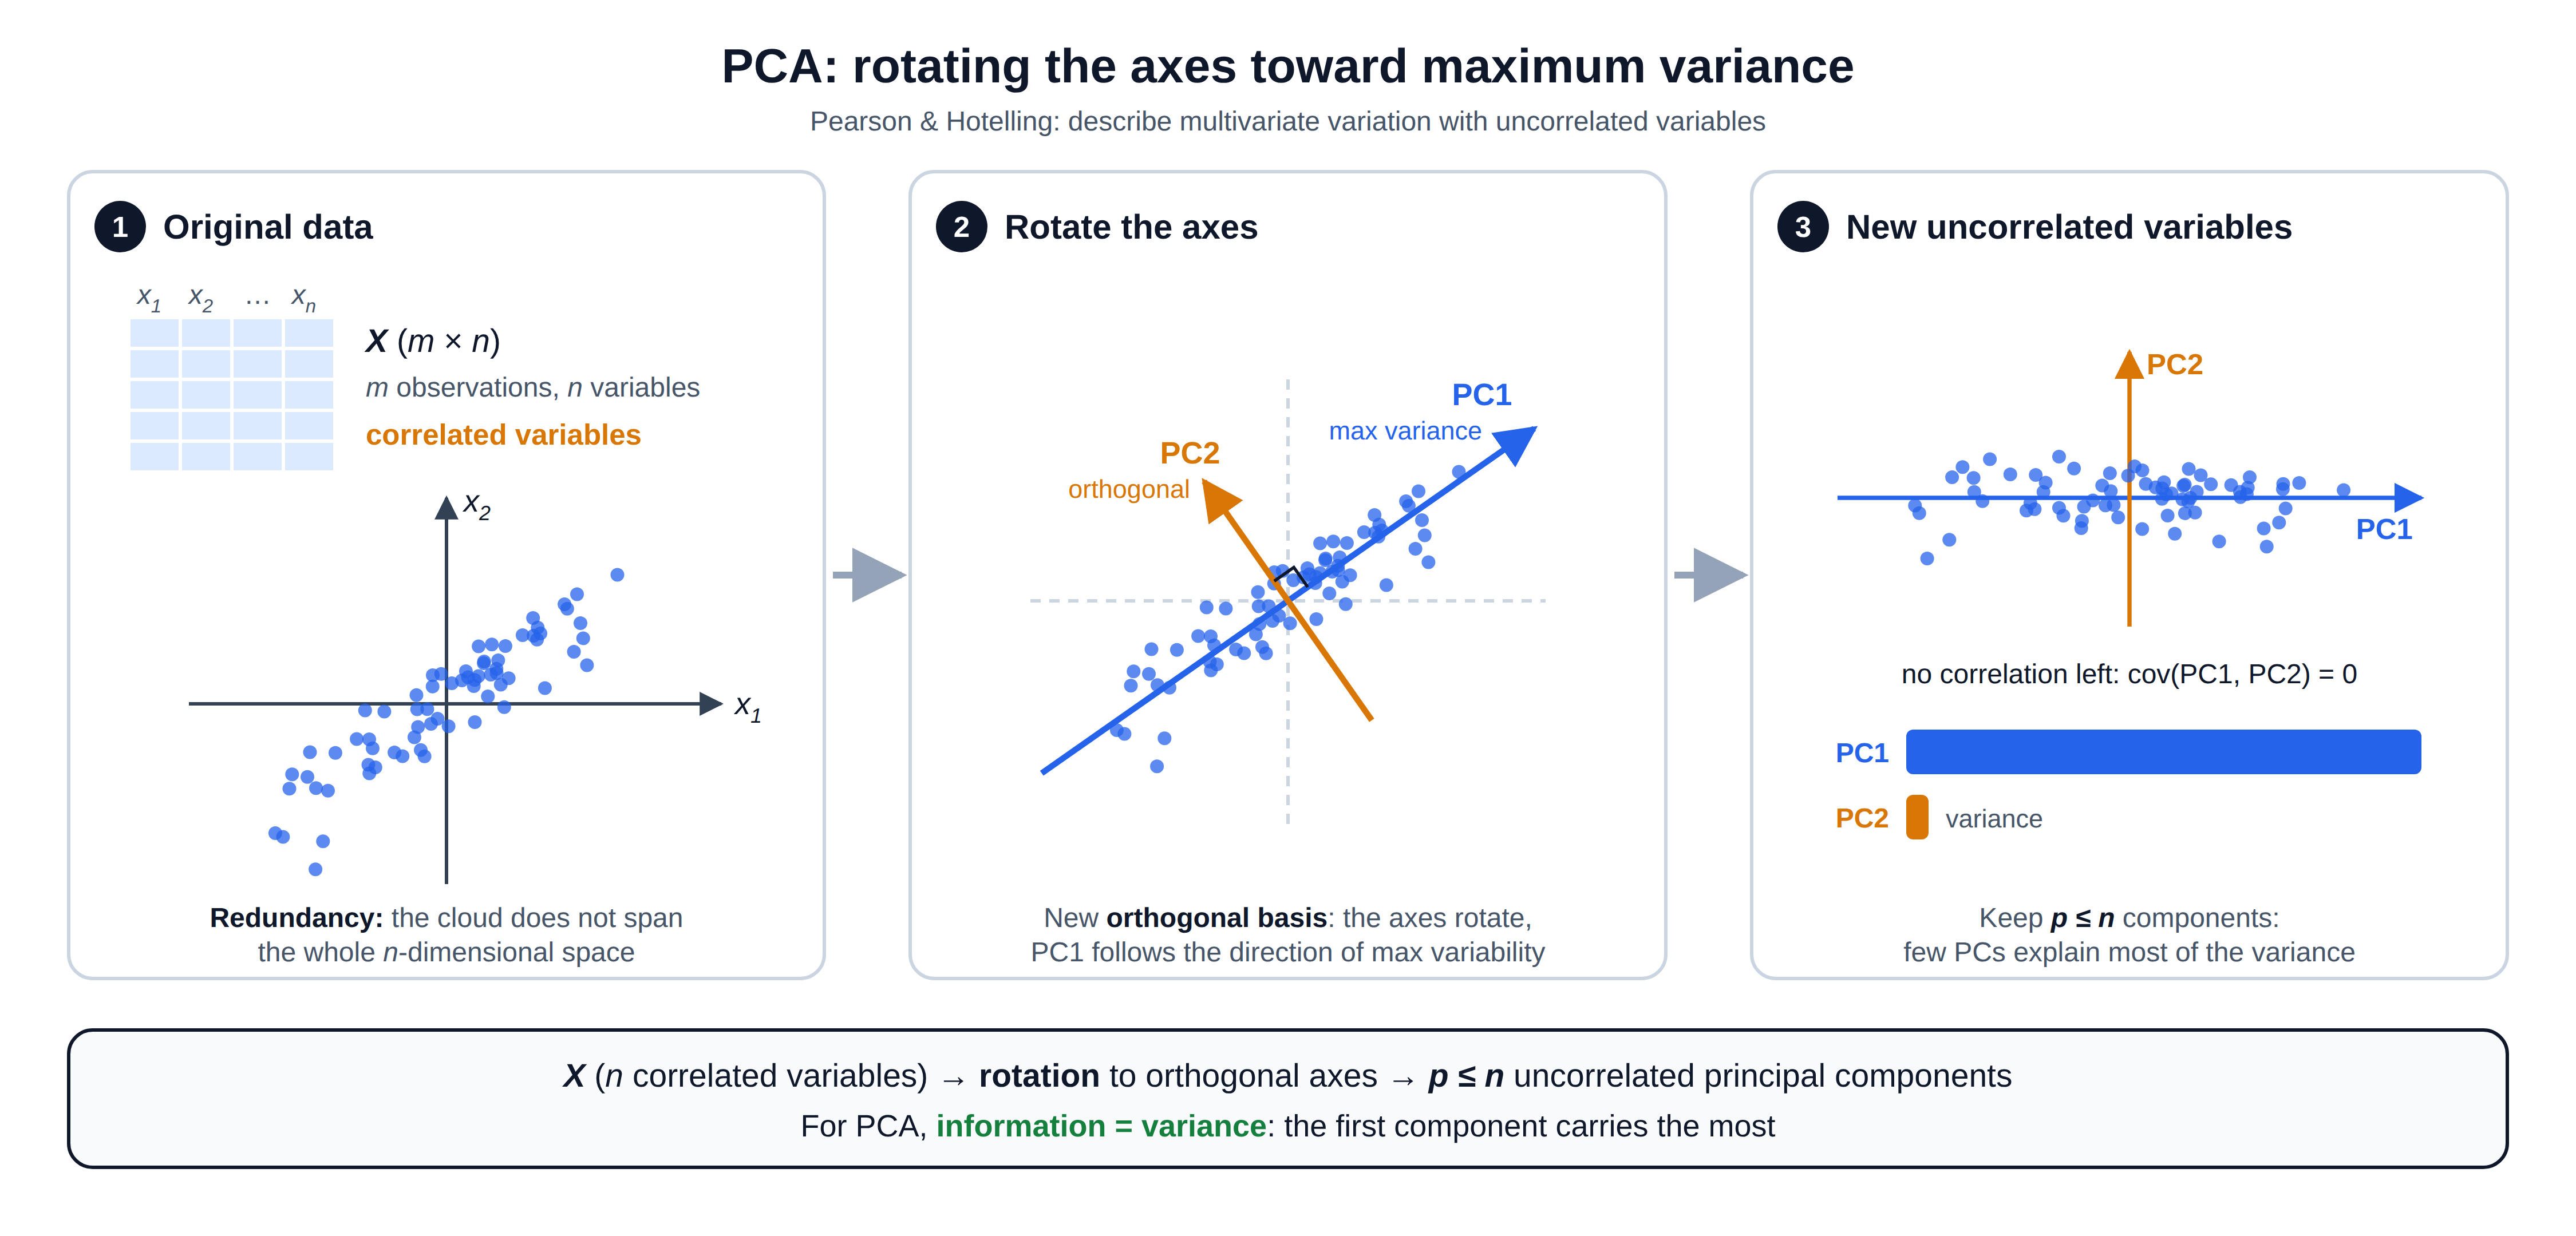
\includegraphics[width=1\textwidth]{images/chapter_4/pca_rotation_axes.png}
    \caption{PCA as a rotation of the axes toward maximum variance}
\end{figure}

In a nutshell, PCA is a \textbf{rotation of the existing axes}. The data points do not move; we only look at them from a new viewpoint. The new axes are \textbf{orthogonal} and point in the directions of \underline{maximum variability}.

\subsection{PCA: Definition}
PCA has two equivalent definitions (see the figure below: data points in red, principal subspace in magenta, projection errors in blue):

\begin{itemize}
    \item \textbf{Maximum variance}: find a lower-dimensional space, called the \emph{principal subspace}, such that the orthogonal projections of the data points onto it are \textbf{as spread out as possible}, i.e.\ have \textbf{maximum variance}.
    \item \textbf{Minimum error}: find the subspace that \textbf{minimizes the sum of the squared projection errors}, i.e.\ of the squared distances of the points from the new axis.
\end{itemize}

\textbf{Why are they equivalent?} For each point, the distance from the mean is fixed and, by Pythagoras, $\text{distance}^2 = \text{projection}^2 + \text{error}^2$. Since the left side does not depend on the chosen axis, \emph{making the projections as long as possible} is the same as \emph{making the errors as short as possible}. The error is exactly what we lose when we rebuild $x'$ from its projection. So PCA also \textbf{minimizes the reconstruction error} between $x'$ and $x$, and can be seen either as a maximization or as a minimization problem.

\begin{figure}[h]
    \centering
    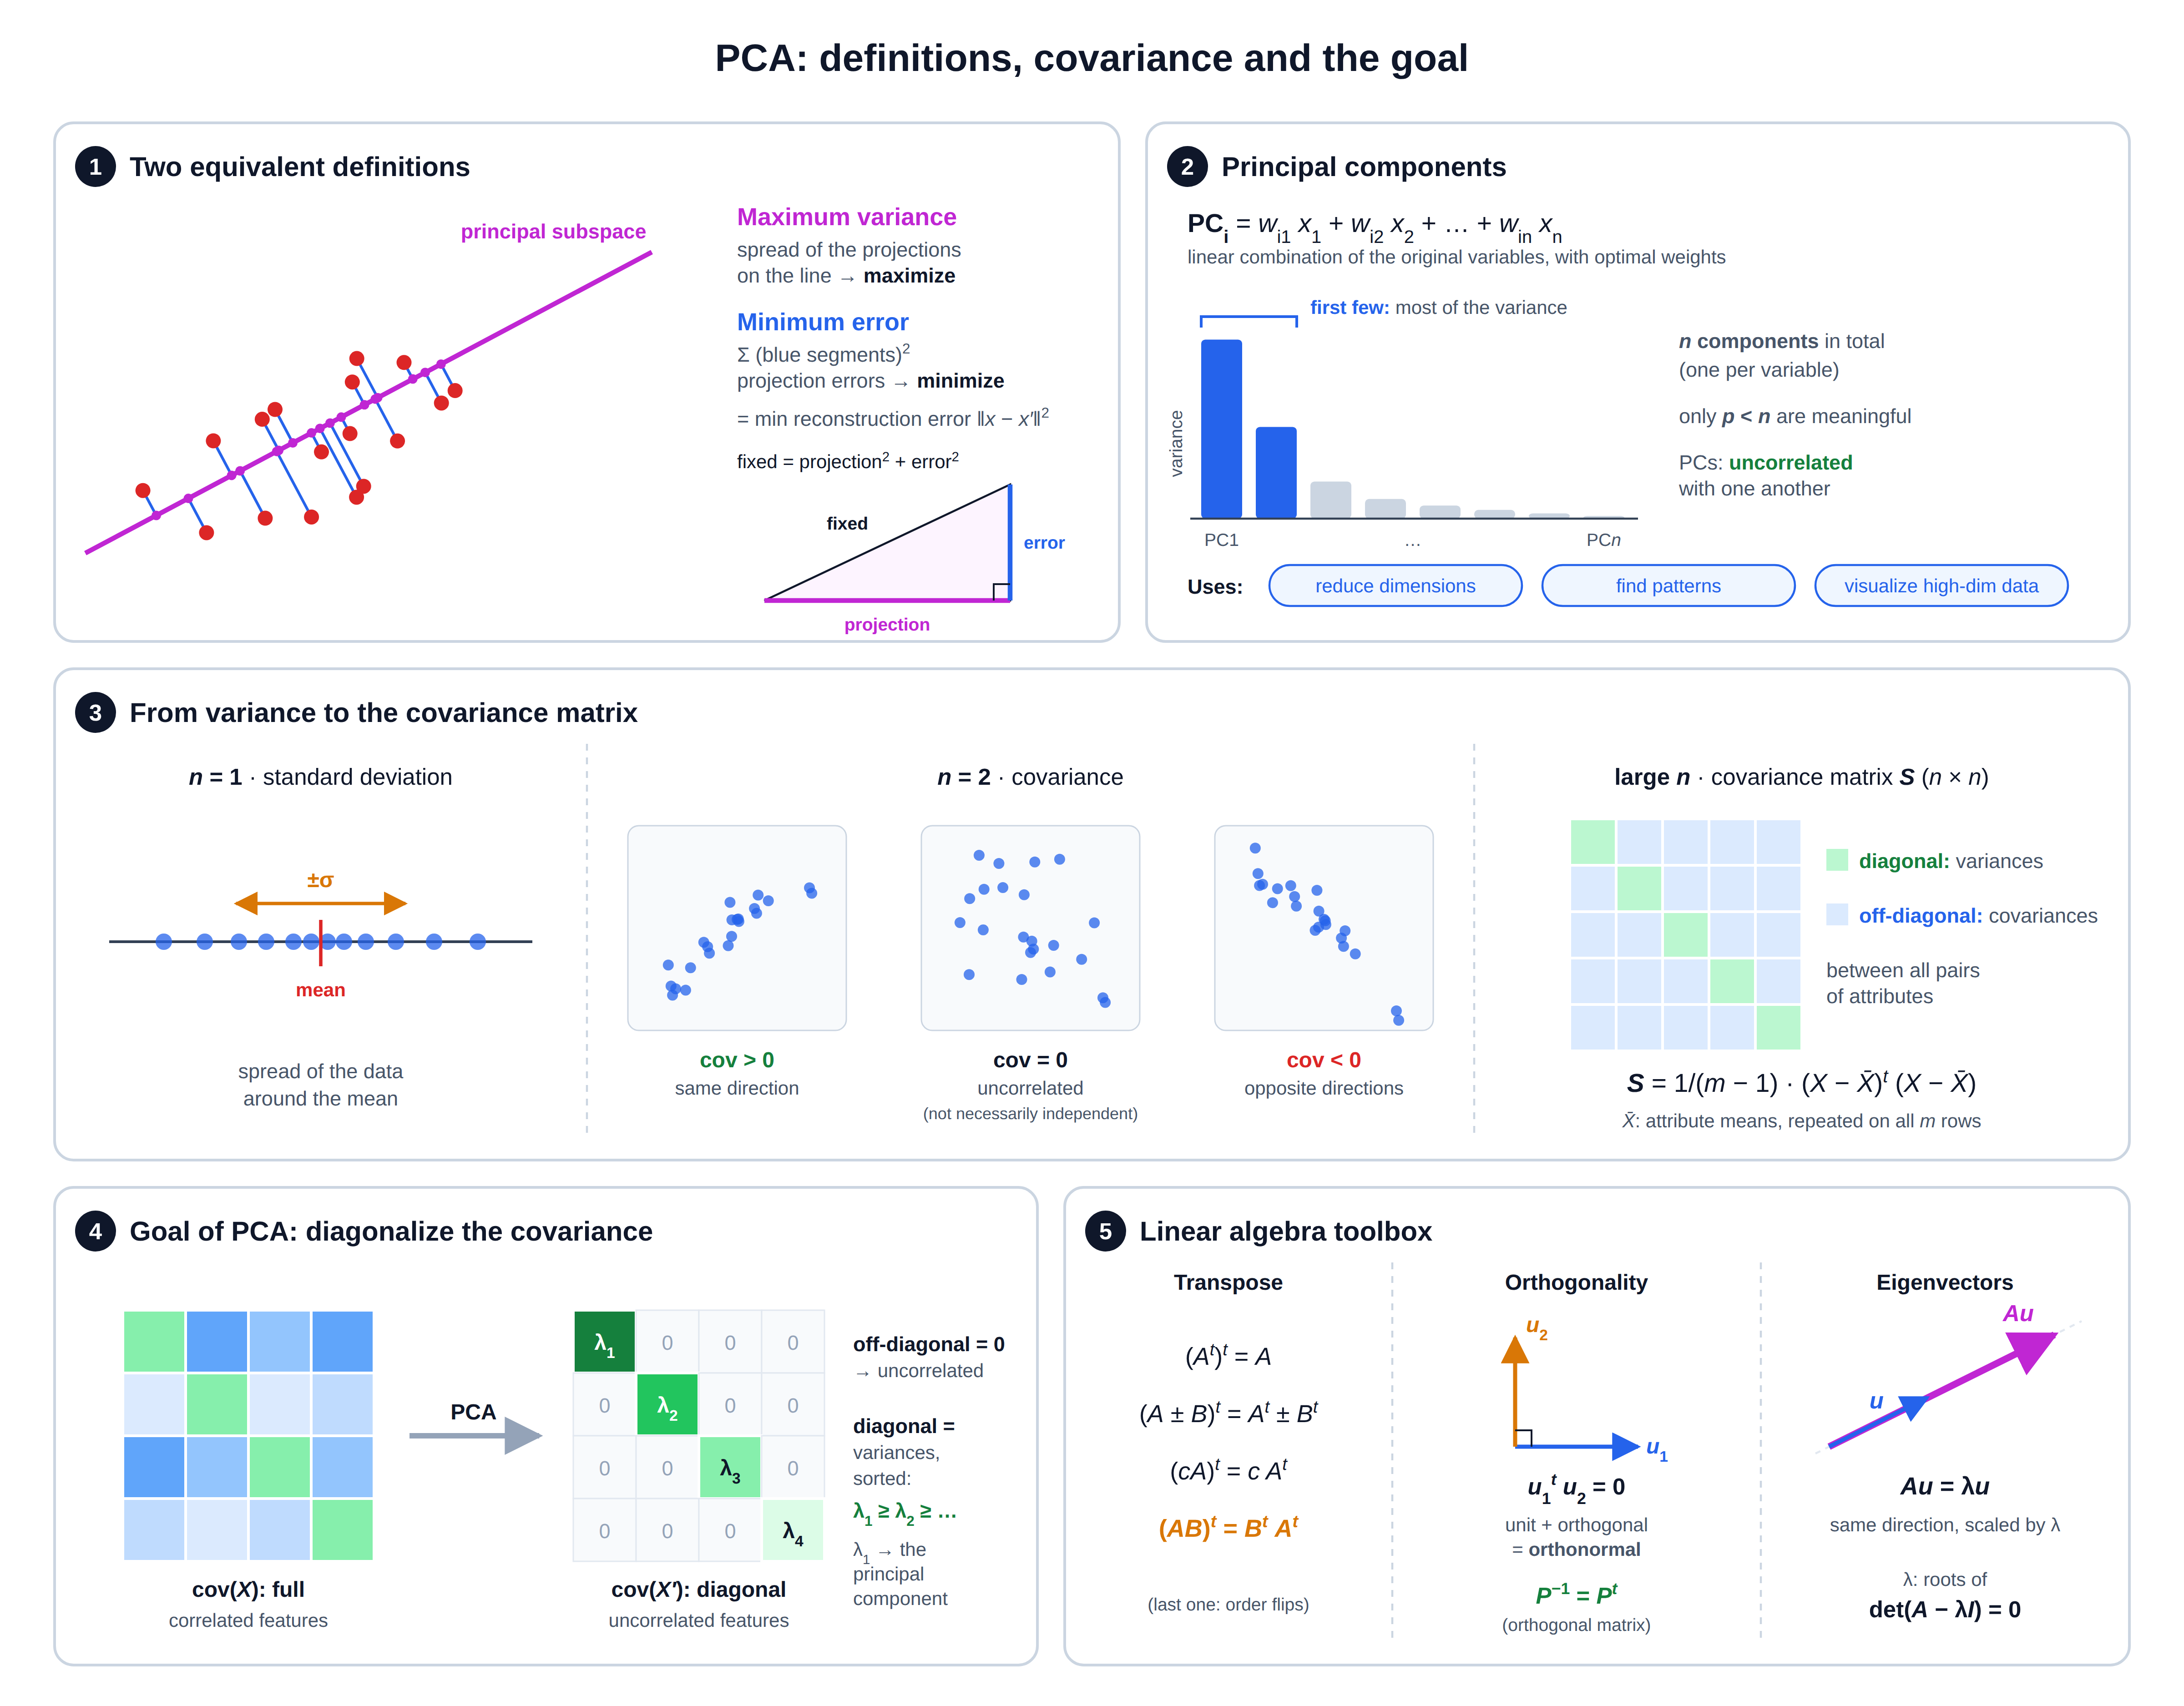
\includegraphics[width=1\textwidth]{images/chapter_4/pca_definitions_covariance.png}
    \caption{PCA definitions, from variance to covariance, and linear algebra remarks}
\end{figure}

A Principal Component is a \textbf{linear combination} of the observed variables with optimal weights:
\[
    \text{PC}_i = w_{i1}x_1 + w_{i2}x_2 + \dots + w_{in}x_n
\]
The weight vector $(w_{i1}, \dots, w_{in})$ is the \emph{direction} of the $i$-th new axis. As many components can be extracted as there are variables ($n$), but usually only the \textbf{first few account for a meaningful amount of variance} ($p < n$). Each component is correlated, to varying degrees, with some of the original variables (those with large weights). However, the components are \textbf{completely uncorrelated with one another}.

PCA can be used to:
\begin{itemize}
    \item Reduce the number of dimensions in data.
    \item Find patterns in high-dimensional data.
    \item Visualize high-dimensional data.
\end{itemize}

\paragraph{From variance to the covariance matrix.}
To find the directions of maximum variance, we first need a tool that describes how the data vary along \emph{every} direction:
\begin{itemize}
    \item With a single attribute ($n=1$), the \textbf{standard deviation} (or its square, the variance) measures how far the data are spread around the mean.
    \item With two attributes ($n=2$), the \textbf{covariance} measures how $x$ and $y$ vary together. If $\operatorname{cov}(x,y) > 0$ they move in the same direction, and if $\operatorname{cov}(x,y) < 0$ they move in opposite directions. If $\operatorname{cov}(x,y) = 0$ they are \emph{uncorrelated}: there is no linear relationship, though they are not necessarily independent.
    \item For a large $n$, all this information is collected in the \textbf{covariance matrix}. It has the variance of each attribute on the diagonal and the covariance of each pair of attributes off the diagonal.
\end{itemize}

\begin{figure}[h!]
    \centering
    \begin{minipage}{0.8\textwidth}
    The sample covariance matrix $S$ ($n \times n$) of $X$ ($m \times n$) is:
    \[
        S = \frac{1}{m-1} (X - \overline{X})^t (X - \overline{X})
    \]
    where $\overline{X}$ is the $m \times n$ matrix of the attribute means: all its $m$ rows are equal to the mean of the rows of $X$. For example, with $n=2$:
    \[
        S = \begin{pmatrix} \operatorname{var}(x_1) & \operatorname{cov}(x_1,x_2) \\ \operatorname{cov}(x_2,x_1) & \operatorname{var}(x_2) \end{pmatrix}
    \]
    $S$ is always \textbf{symmetric}, since $\operatorname{cov}(x_1,x_2) = \operatorname{cov}(x_2,x_1)$.
    \end{minipage}
    \caption{Covariance Matrix}
\end{figure}

\begin{figure}[h]
    \centering
    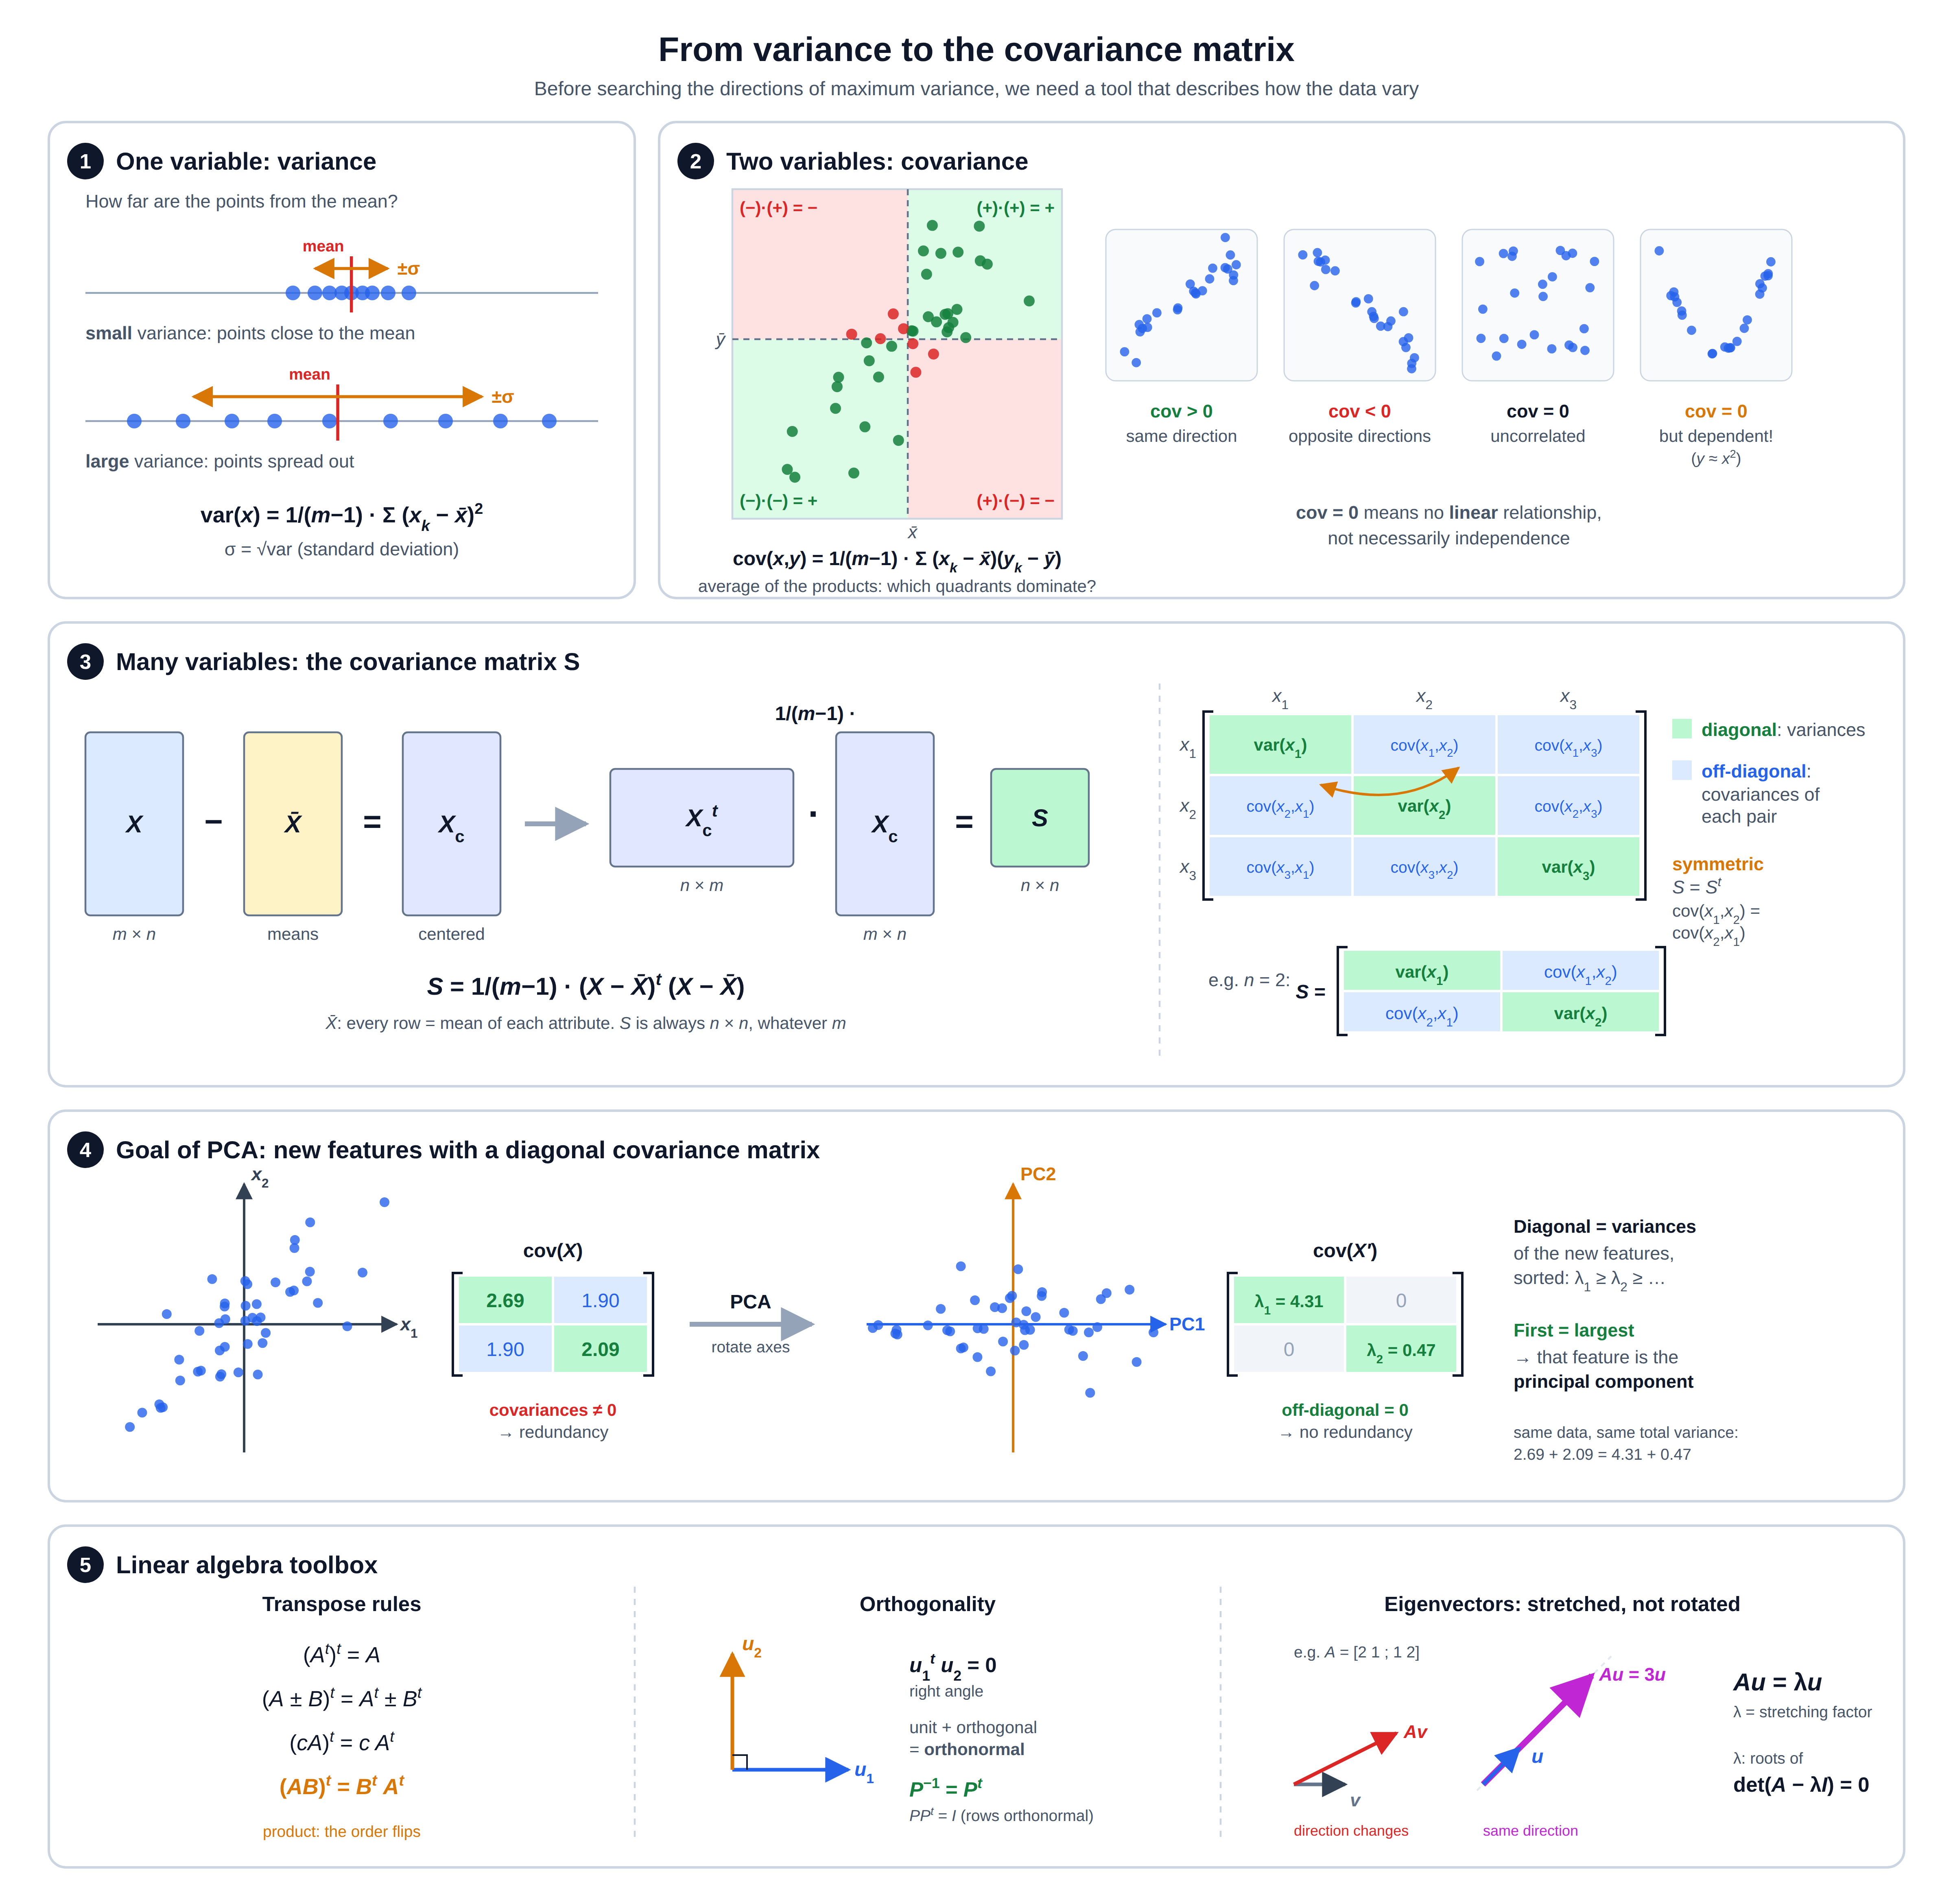
\includegraphics[width=1\textwidth]{images/chapter_4/covariance_matrix_explained.png}
    \caption{From variance to the covariance matrix, the goal of PCA and linear algebra remarks}
\end{figure}

\textbf{Goal of PCA}: find new features whose covariance matrix is \textbf{diagonal}:
\begin{itemize}
    \item off-diagonal entries equal to 0 mean the new features are pairwise uncorrelated, so there is no redundancy left;
    \item the diagonal holds their variances, sorted so that the \textbf{first one is the largest possible}; that feature is the principal component.
\end{itemize}

Useful matrix remarks:

\begin{figure}[h!]
    \centering
    \begin{minipage}{0.6\textwidth}
    If $A$ and $B$ are matrices whose sizes make the operations defined, and $c$ is any scalar:
    \begin{align*}
        (A^t)^t &= A \\
        (A \pm B)^t &= A^t \pm B^t \\
        (cA)^t &= cA^t \\
        (AB)^t &= B^t A^t
    \end{align*}
    \end{minipage}
    \caption{Matrix Remarks}
\end{figure}

Orthogonality and eigenvalue remarks:

\begin{itemize}
    \item Two vectors $u_1$ and $u_2$ are \textbf{orthogonal} if $u_1^t u_2 = 0$ (they form a right angle).
    \item Orthogonal unit vectors are called \textbf{orthonormal}.
    \item A matrix whose rows are orthonormal is \textbf{orthogonal}, and its inverse is its transpose: $P^{-1} = P^t$, i.e.\ $PP^t = I$.
    \item Vectors $u$ such that $Au$ has the same direction as $u$ are the \textbf{eigenvectors} of $A$: the matrix only stretches them, without rotating them.
    \item In $Au = \lambda u$, the stretching factor $\lambda$ is the corresponding \textbf{eigenvalue} of $A$.
    \item The eigenvalues are the roots of $\det(A - \lambda I) = 0$.
\end{itemize}

\section{PCA: orthonormal change of basis P}

\paragraph{What does a change of basis mean?}
Let $u$ be a unit vector representing a new axis. The coordinate of a data point $x$ along that axis is its \textbf{projection}, i.e.\ the dot product of $x$ and $u$. If we stack the $n$ new axes $u_1, \dots, u_n$ as the \emph{rows} of a matrix $P$, all the projections are computed at once:
\[
    X' = XP^t \qquad \text{entry } (i,j) \text{ of } X' = \text{coordinate of point } i \text{ along axis } u_j
\]
$X'$ contains the \emph{same points} as $X$, only described in the new coordinate system. PCA must therefore:

\begin{itemize}
    \item Choose an \textbf{orthonormal} basis $P$, i.e.\ new axes that are perpendicular unit vectors, so that the transformation is a pure rotation.
    \item Choose it so that $\operatorname{cov}(X')$ is \textbf{diagonal}, i.e.\ the new variables are uncorrelated.
    \item Keep the first $p$ rows of $P$ as the \textbf{principal components} of $X$.
\end{itemize}

\begin{figure}[h]
    \centering
    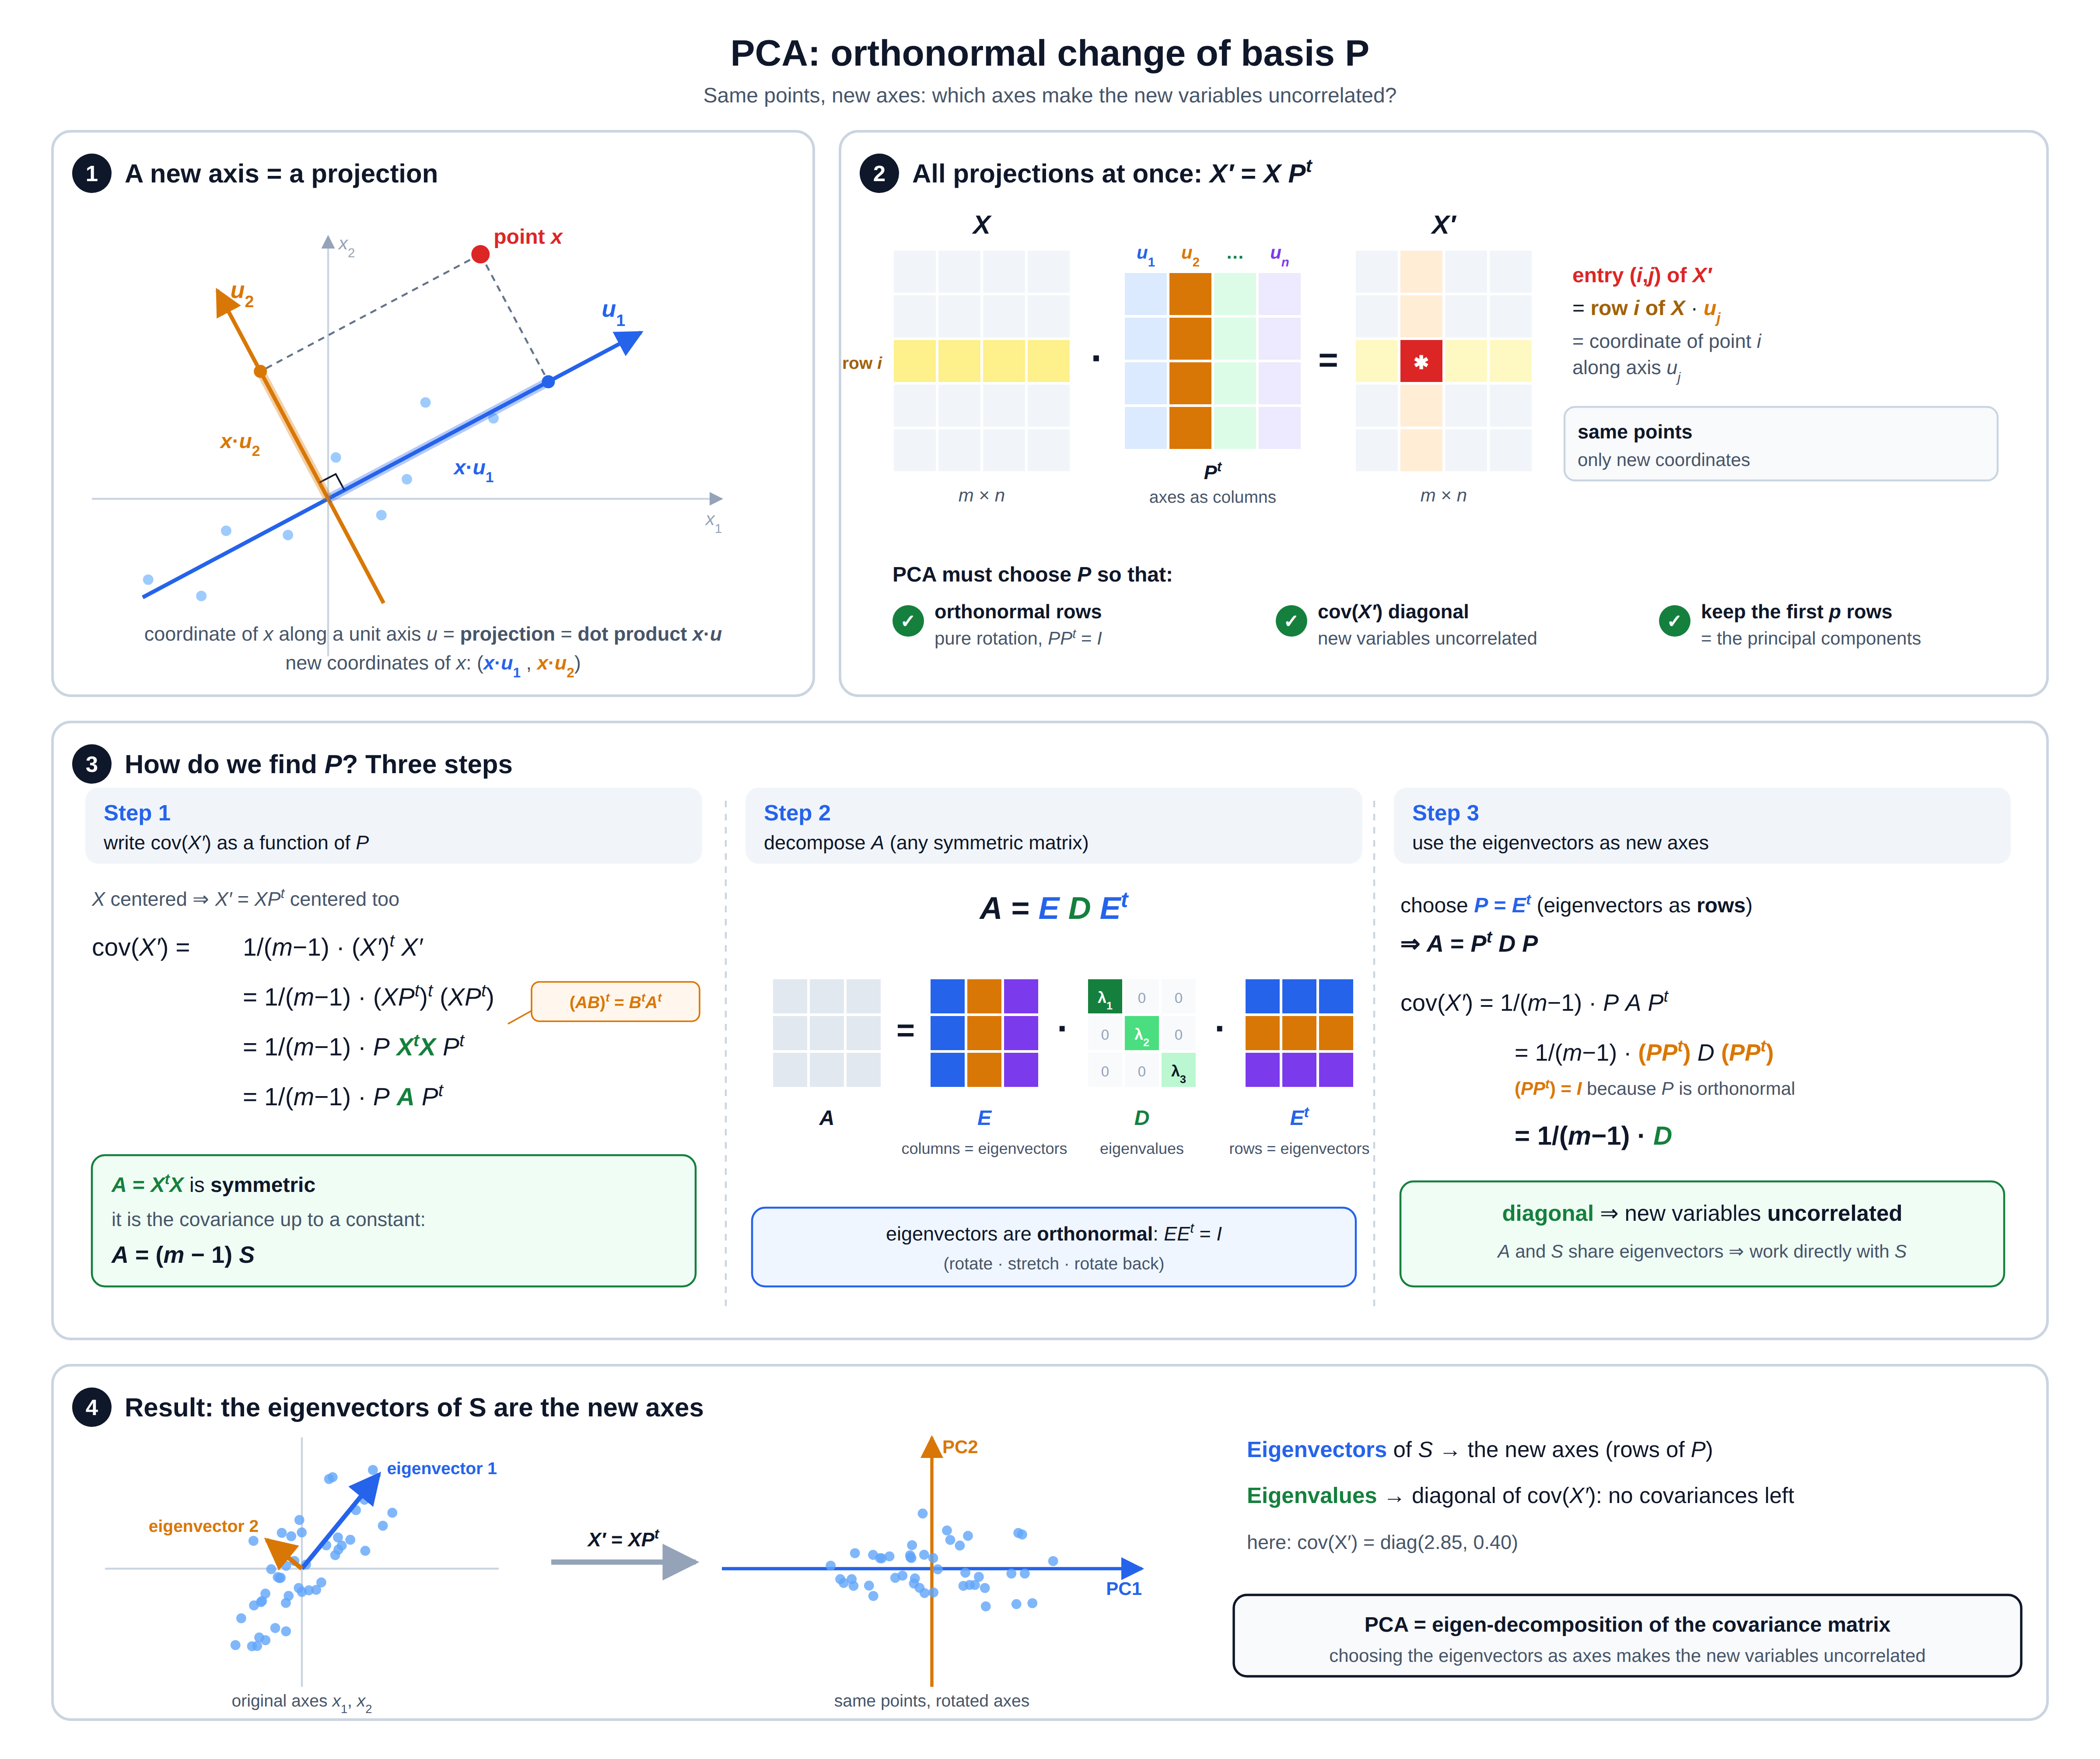
\includegraphics[width=1\textwidth]{images/chapter_4/pca_change_of_basis.png}
    \caption{Change of basis $X' = XP^t$ and why the eigenvectors diagonalize $\operatorname{cov}(X')$}
\end{figure}

\textbf{How do we find such a $P$?}

\textbf{Step 1: write $\operatorname{cov}(X')$ as a function of $P$.} Assume $X$ is centered (zero mean); then $X' = XP^t$ is centered too, and its covariance is simply $\frac{1}{m-1}(X')^tX'$. Substituting $X' = XP^t$ and using $(AB)^t = B^tA^t$:
\[
    \operatorname{cov}(X') = \frac{1}{m-1} (XP^t)^t (XP^t) = \frac{1}{m-1} P \,\underbrace{X^t X}_{A}\, P^t = \frac{1}{m-1} P A P^t
\]
The matrix $A = X^tX$ is \textbf{symmetric} and is just the covariance of the original data up to a constant: $A = (m-1)S$.

\textbf{Step 2: decompose $A$.} Every symmetric matrix can be written as
\[
    A = E D E^t
\]
where the columns of $E$ are the (orthonormal) \textbf{eigenvectors} of $A$ and $D$ is the diagonal matrix of its \textbf{eigenvalues}.

\textbf{Step 3: choose the eigenvectors as new axes.} Set $P = E^t$, so that the eigenvectors become the \emph{rows} of $P$. Then $A = P^t D P$ and, since $PP^t = I$:
\[
    \operatorname{cov}(X') = \frac{1}{m-1} \underbrace{P P^t}_{I} D \underbrace{P P^t}_{I} = \frac{1}{m-1} D
\]
which is \textbf{diagonal}. Therefore, using the eigenvectors as new axes makes the new variables uncorrelated. Since $A$ and $S$ differ only by a constant, they have the same eigenvectors, so in practice we work directly with $S$.

\paragraph{Why do the eigenvalues give the variance?}
The variance of the (centered) data projected on a unit vector $u$ is
\[
    \operatorname{var}(Xu) = \frac{1}{m-1}(Xu)^t(Xu) = u^t S u
\]
If $u$ is an eigenvector of $S$ ($Su = \lambda u$), this becomes $u^t \lambda u = \lambda$, because $u^tu = 1$. So \textbf{each eigenvalue is the variance of the data along its eigenvector}. The direction with the largest variance is therefore the eigenvector with the largest eigenvalue (the formal proof of the maximization is omitted).

\begin{figure}[h]
    \centering
    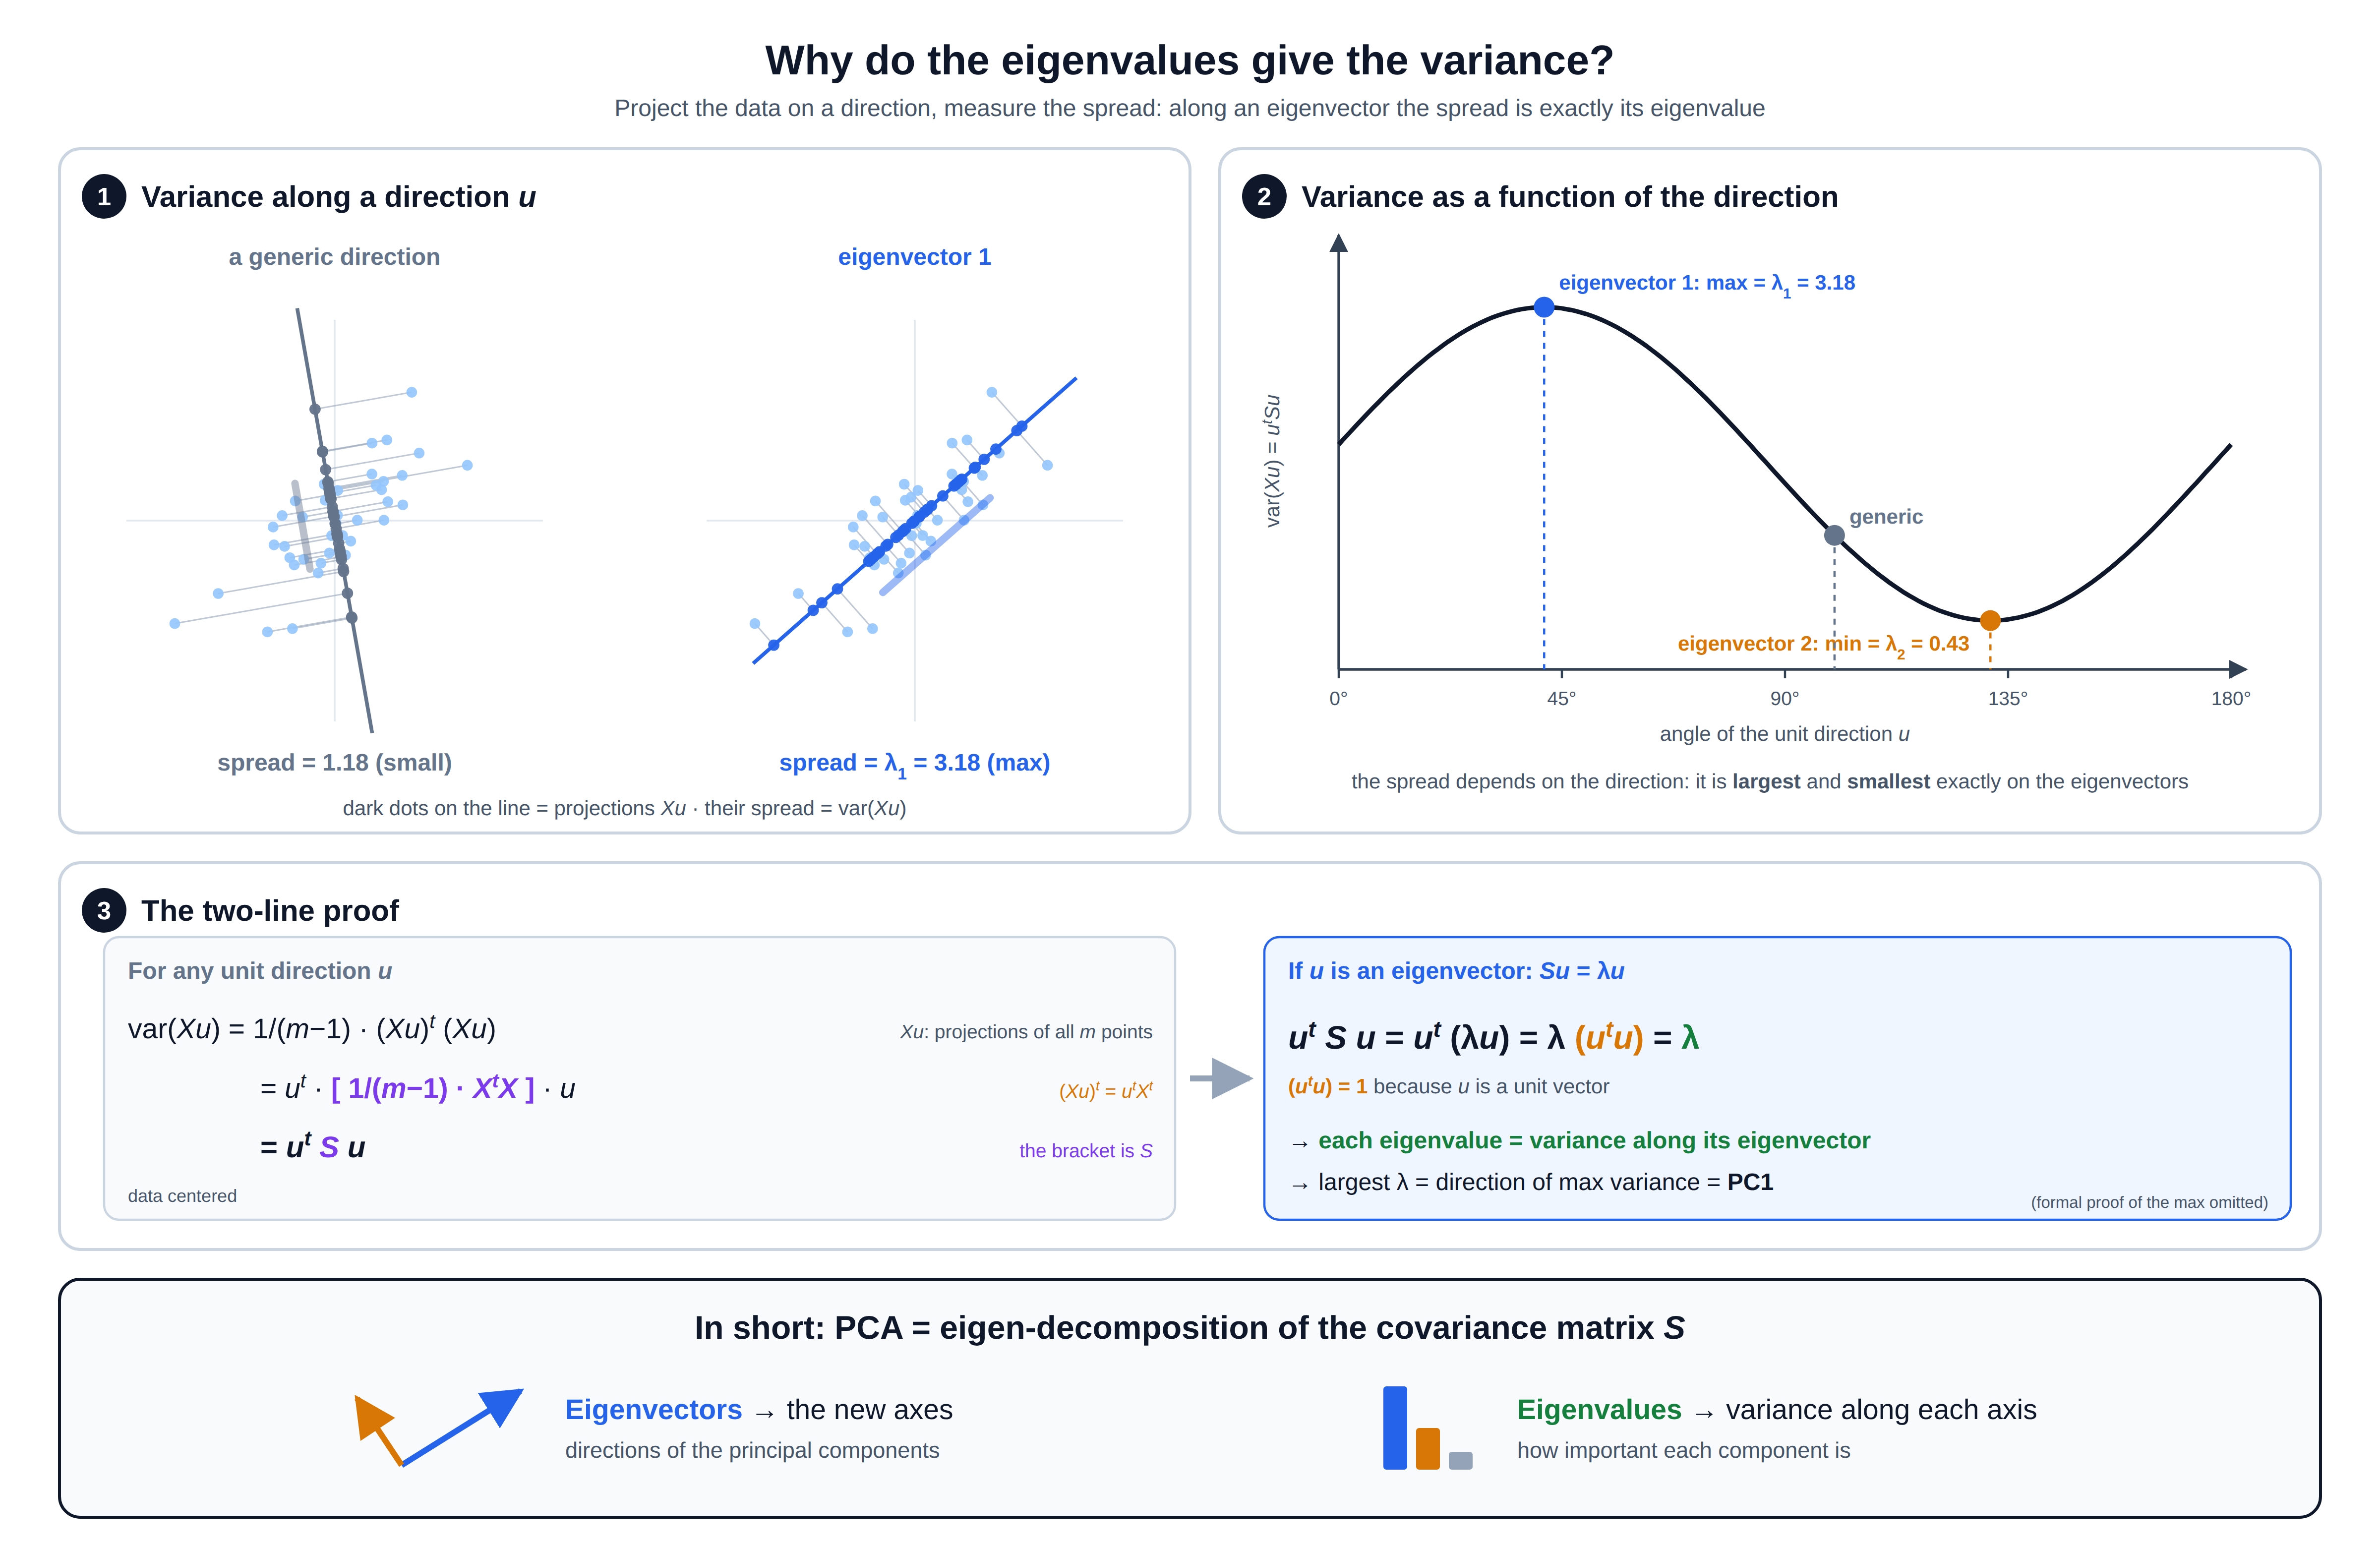
\includegraphics[width=1\textwidth]{images/chapter_4/pca_eigenvalues_variance.png}
    \caption{Each eigenvalue is the variance of the data along its eigenvector}
\end{figure}

\begin{center}
    \fbox{\parbox{0.9\textwidth}{\centering
    \textbf{In short}: PCA $=$ eigen-decomposition of the covariance matrix.\\
    \textbf{Eigenvectors} $\rightarrow$ the new axes (the directions of the principal components).\\
    \textbf{Eigenvalues} $\rightarrow$ the variance along each axis (how important it is).}}
\end{center}

\subsection{Principal Components}
\begin{itemize}
    \item \textbf{PC1} is the eigenvector with the \textbf{largest eigenvalue}: the direction along which the data have the \textbf{greatest variance}.
    \item \textbf{PC2} is the eigenvector with the second largest eigenvalue: the direction of maximum variance \emph{left} in the data, \textbf{orthogonal to PC1}.
    \item The remaining PCs follow in the same way, in order of decreasing eigenvalue.
\end{itemize}

\section{Steps of PCA}
To recap, PCA follows these steps:

\begin{enumerate}
    \item \textbf{Center the data}: subtract the mean of each attribute, $X - \overline{X}$, so that every column has zero mean.
    \item \textbf{Compute the covariance matrix} $S$ ($n \times n$) of the centered data.
    \item \textbf{Find the eigenvectors and eigenvalues} of $S$: each eigenvector is a new axis, and its eigenvalue $\lambda$ is the variance along it.
    \item \textbf{Sort} the eigenvectors by decreasing $\lambda$, from the most to the least important direction.
    \item \textbf{Select} the eigenvectors of the top $p$ eigenvalues and use them as rows of $P$ ($p \times n$).
    \item \textbf{Project} the data: $X' = XP^t$, an $m \times p$ matrix, i.e.\ the same $m$ points described by only $p$ features.
\end{enumerate}

Since each eigenvalue is a variance, the percentage of the total variance explained by component $i$ is its share of the sum:

\begin{figure}[h]
    \centering
    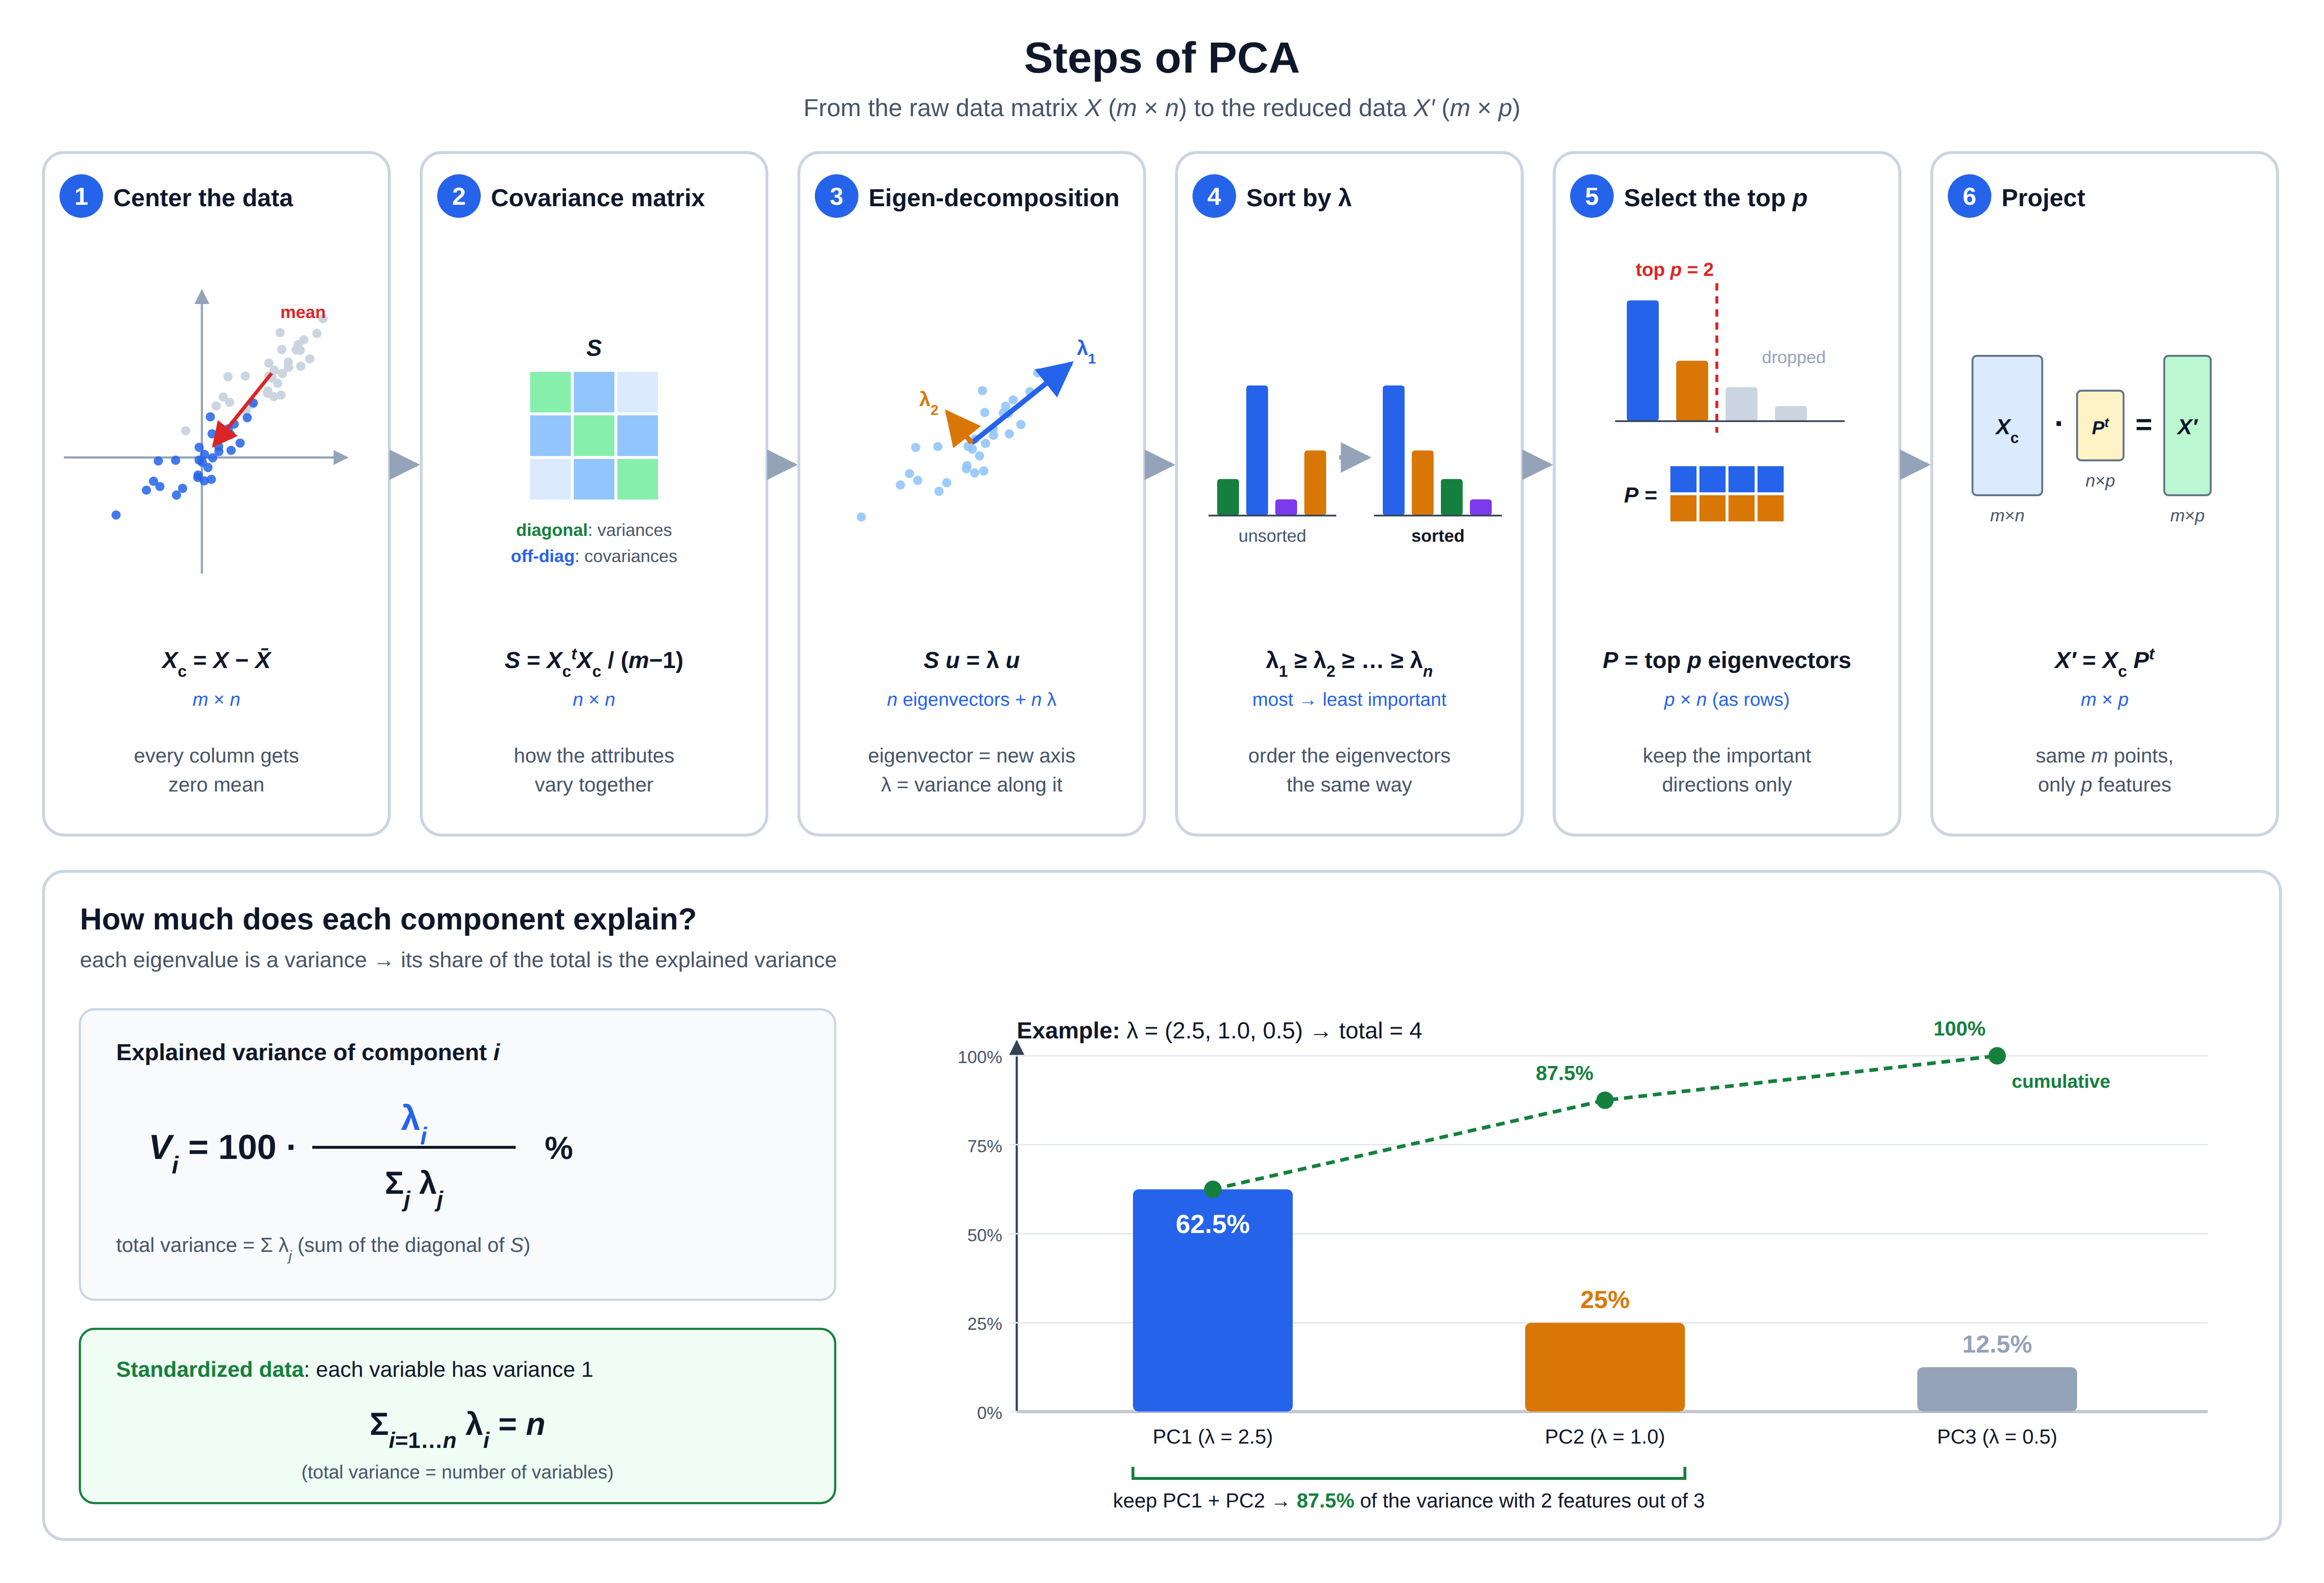
\includegraphics[width=1\textwidth]{images/chapter_4/pca_steps.png}
    \caption{The six steps of PCA and the explained variance}
\end{figure}

\begin{figure}[h!]
    \centering
    \begin{minipage}{0.7\textwidth}
    \[
        V_i = 100 \, \frac{\lambda_i}{\sum_{j=1}^{n} \lambda_j}
    \]
    \[
        \sum_{i=1}^{n} \lambda_i = n \quad \text{(for standardized data: each variable has variance 1)}
    \]
    \emph{Example}: with $\lambda = (2.5,\ 1.0,\ 0.5)$ the total is 4, so PC1 explains $62.5\%$, PC2 $25\%$ and PC3 $12.5\%$. Keeping only PC1 and PC2 preserves $87.5\%$ of the variance.
    \end{minipage}
    \caption{Eigenvalues and Variance}
\end{figure}

\subsection{Properties of Principal Components}
The resulting Principal Components:

\begin{itemize}
    \item are \textbf{linear combinations} of the original variables;
    \item are \textbf{uncorrelated} with each other;
    \item capture \textbf{as much of the original variance as possible}.
\end{itemize}

PCA is \textbf{sensitive to scale}. If one variable is measured in meters and another in millimeters, the second has a much larger variance only because of its unit, and it would dominate PC1. PCA should therefore be applied to variables on approximately the same scale. It is good practice to \textbf{standardize} the data first (zero mean and unit variance for each variable), so that all variables carry the same weight.

\textbf{Choice of $p$} (how many principal components to keep):

\begin{itemize}
    \item \textbf{Kaiser criterion}: keep the PCs with eigenvalue $> 1$. With standardized data each original variable has variance 1, so a PC with $\lambda > 1$ explains more than a single original variable.
    \item \textbf{Proportion of variance explained}: keep PCs until the cumulative explained variance exceeds a threshold (e.g.\ 80--90\%).
    \item \textbf{Elbow method}: plot the eigenvalues in decreasing order (\emph{scree plot}); the point where the curve bends and flattens (the ``elbow'') indicates how many components to retain.
\end{itemize}

\section{Non-linear Dimensionality Reduction}
PCA finds only \emph{linear} axes, so in some cases it does not perform well. For example, circularly-shaped data require \textbf{non-linear axes}.

\begin{figure}[h]
    \centering
    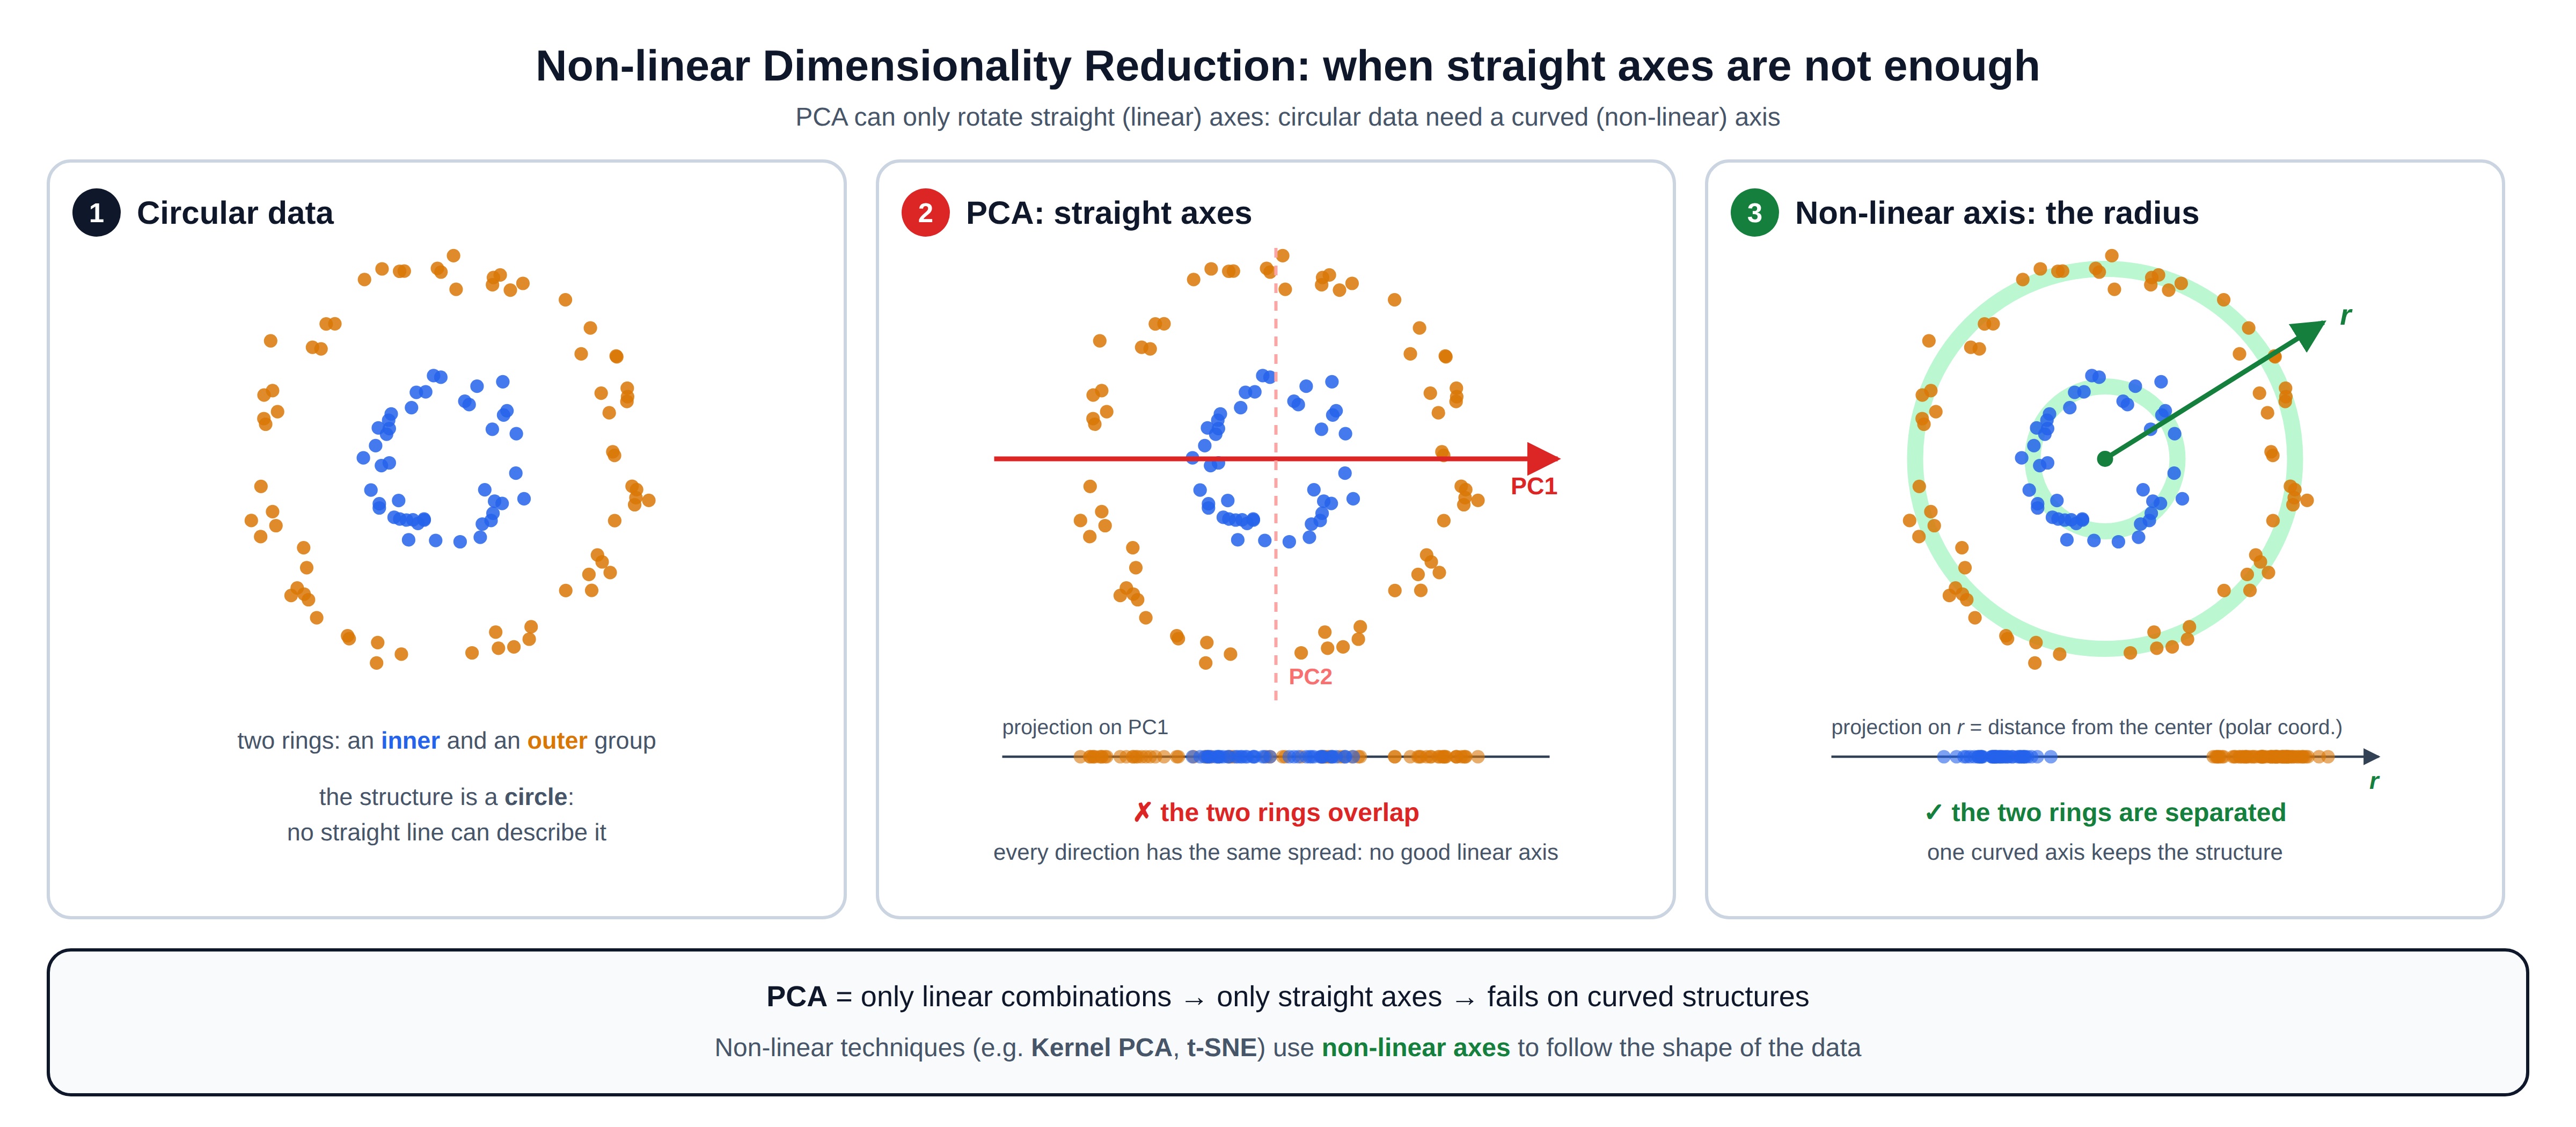
\includegraphics[width=1\textwidth]{images/chapter_4/nonlinear_dr_intro.png}
    \caption{Circular data: PCA's straight axes fail, a non-linear axis (the radius) works}
\end{figure}

\subsection{Kernel PCA}
Kernel PCA extends PCA. Instead of using the points $x$ directly, it maps them to a different feature space $f(x)$, for instance polar coordinates instead of Cartesian ones. PCA is then performed in this new space, giving components that are \textbf{non-linear with respect to the original space}.

\begin{figure}[h!]
    \centering
    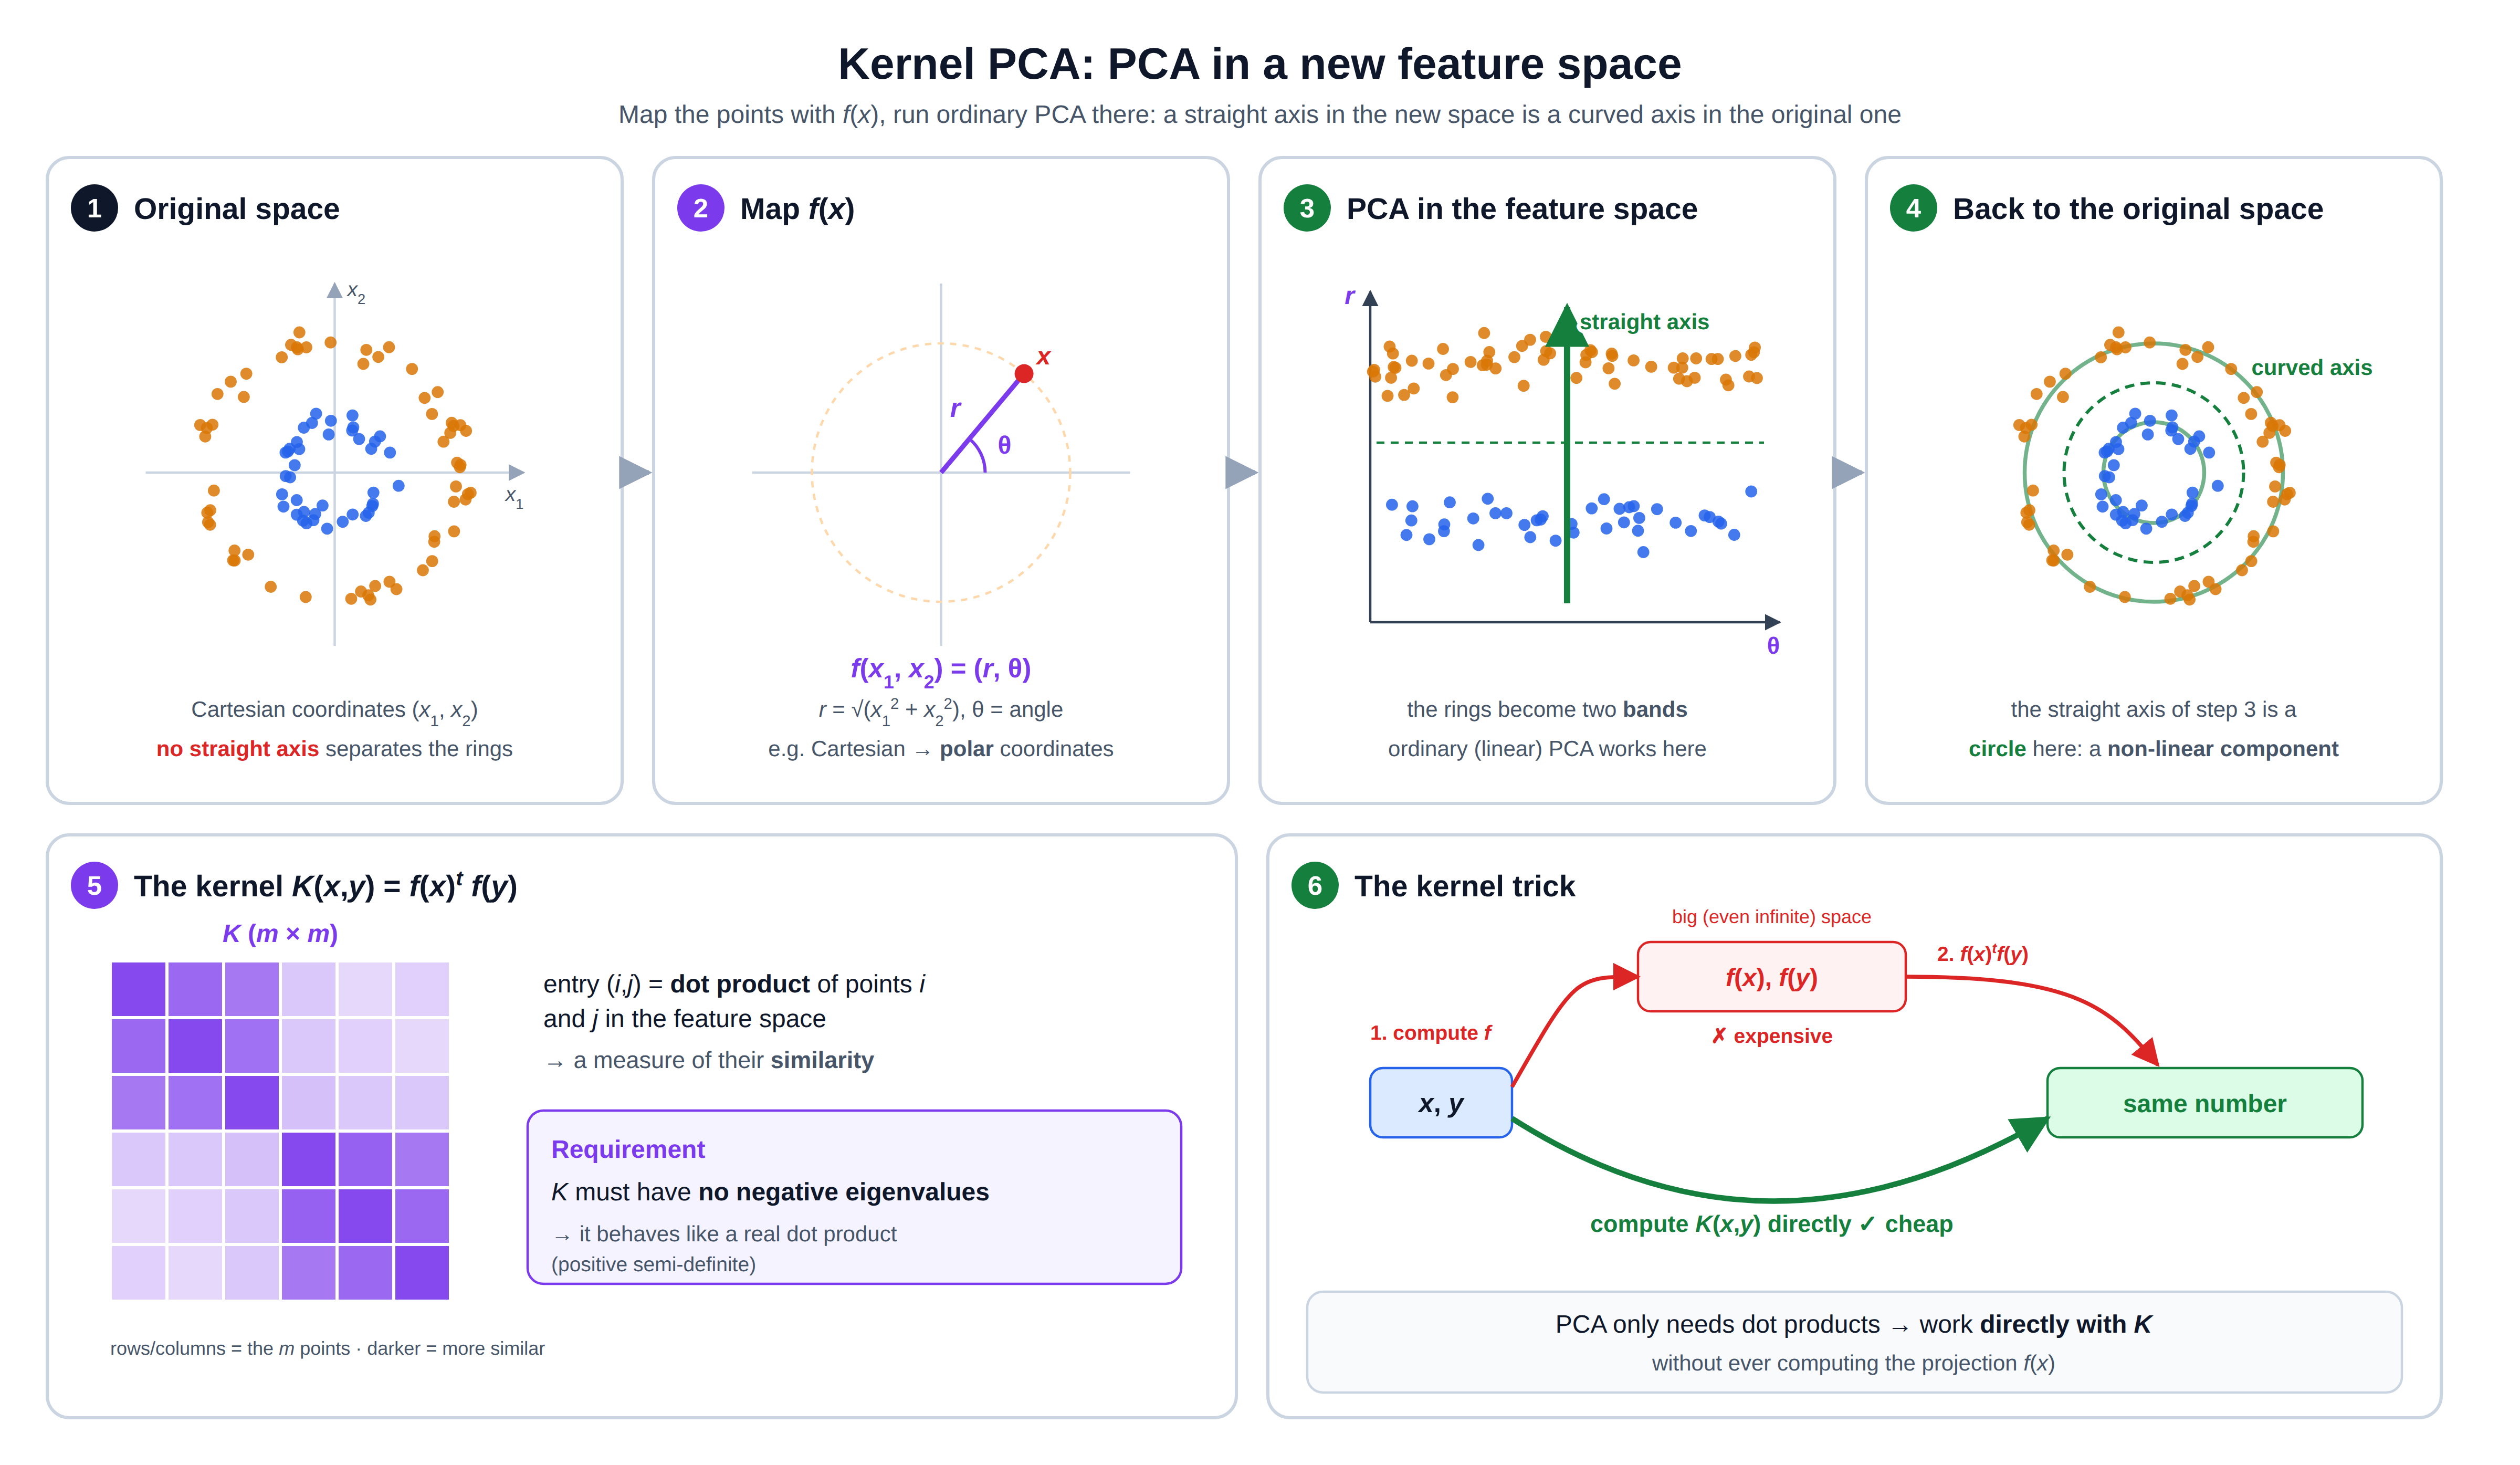
\includegraphics[width=0.5\textwidth]{images/chapter_4/kernel_pca.png}
    \caption{Kernel PCA: PCA in a feature space and the kernel trick}
\end{figure}

The map $f$ must be such that the kernel $K(x, y) = f(x)^t f(y)$ has \textbf{no negative eigenvalues}. In practice one can work \textbf{directly with the kernel matrix $K$}, without explicitly computing the projection $f(x)$ (the \emph{kernel trick}).


\subsection{t-SNE}
t-SNE is a non-linear dimensionality reduction technique designed to \textbf{embed high-dimensional data for visualization}. Similar objects are mapped to nearby points and dissimilar objects to distant points, with high probability.

\begin{figure}[h!]
    \centering
    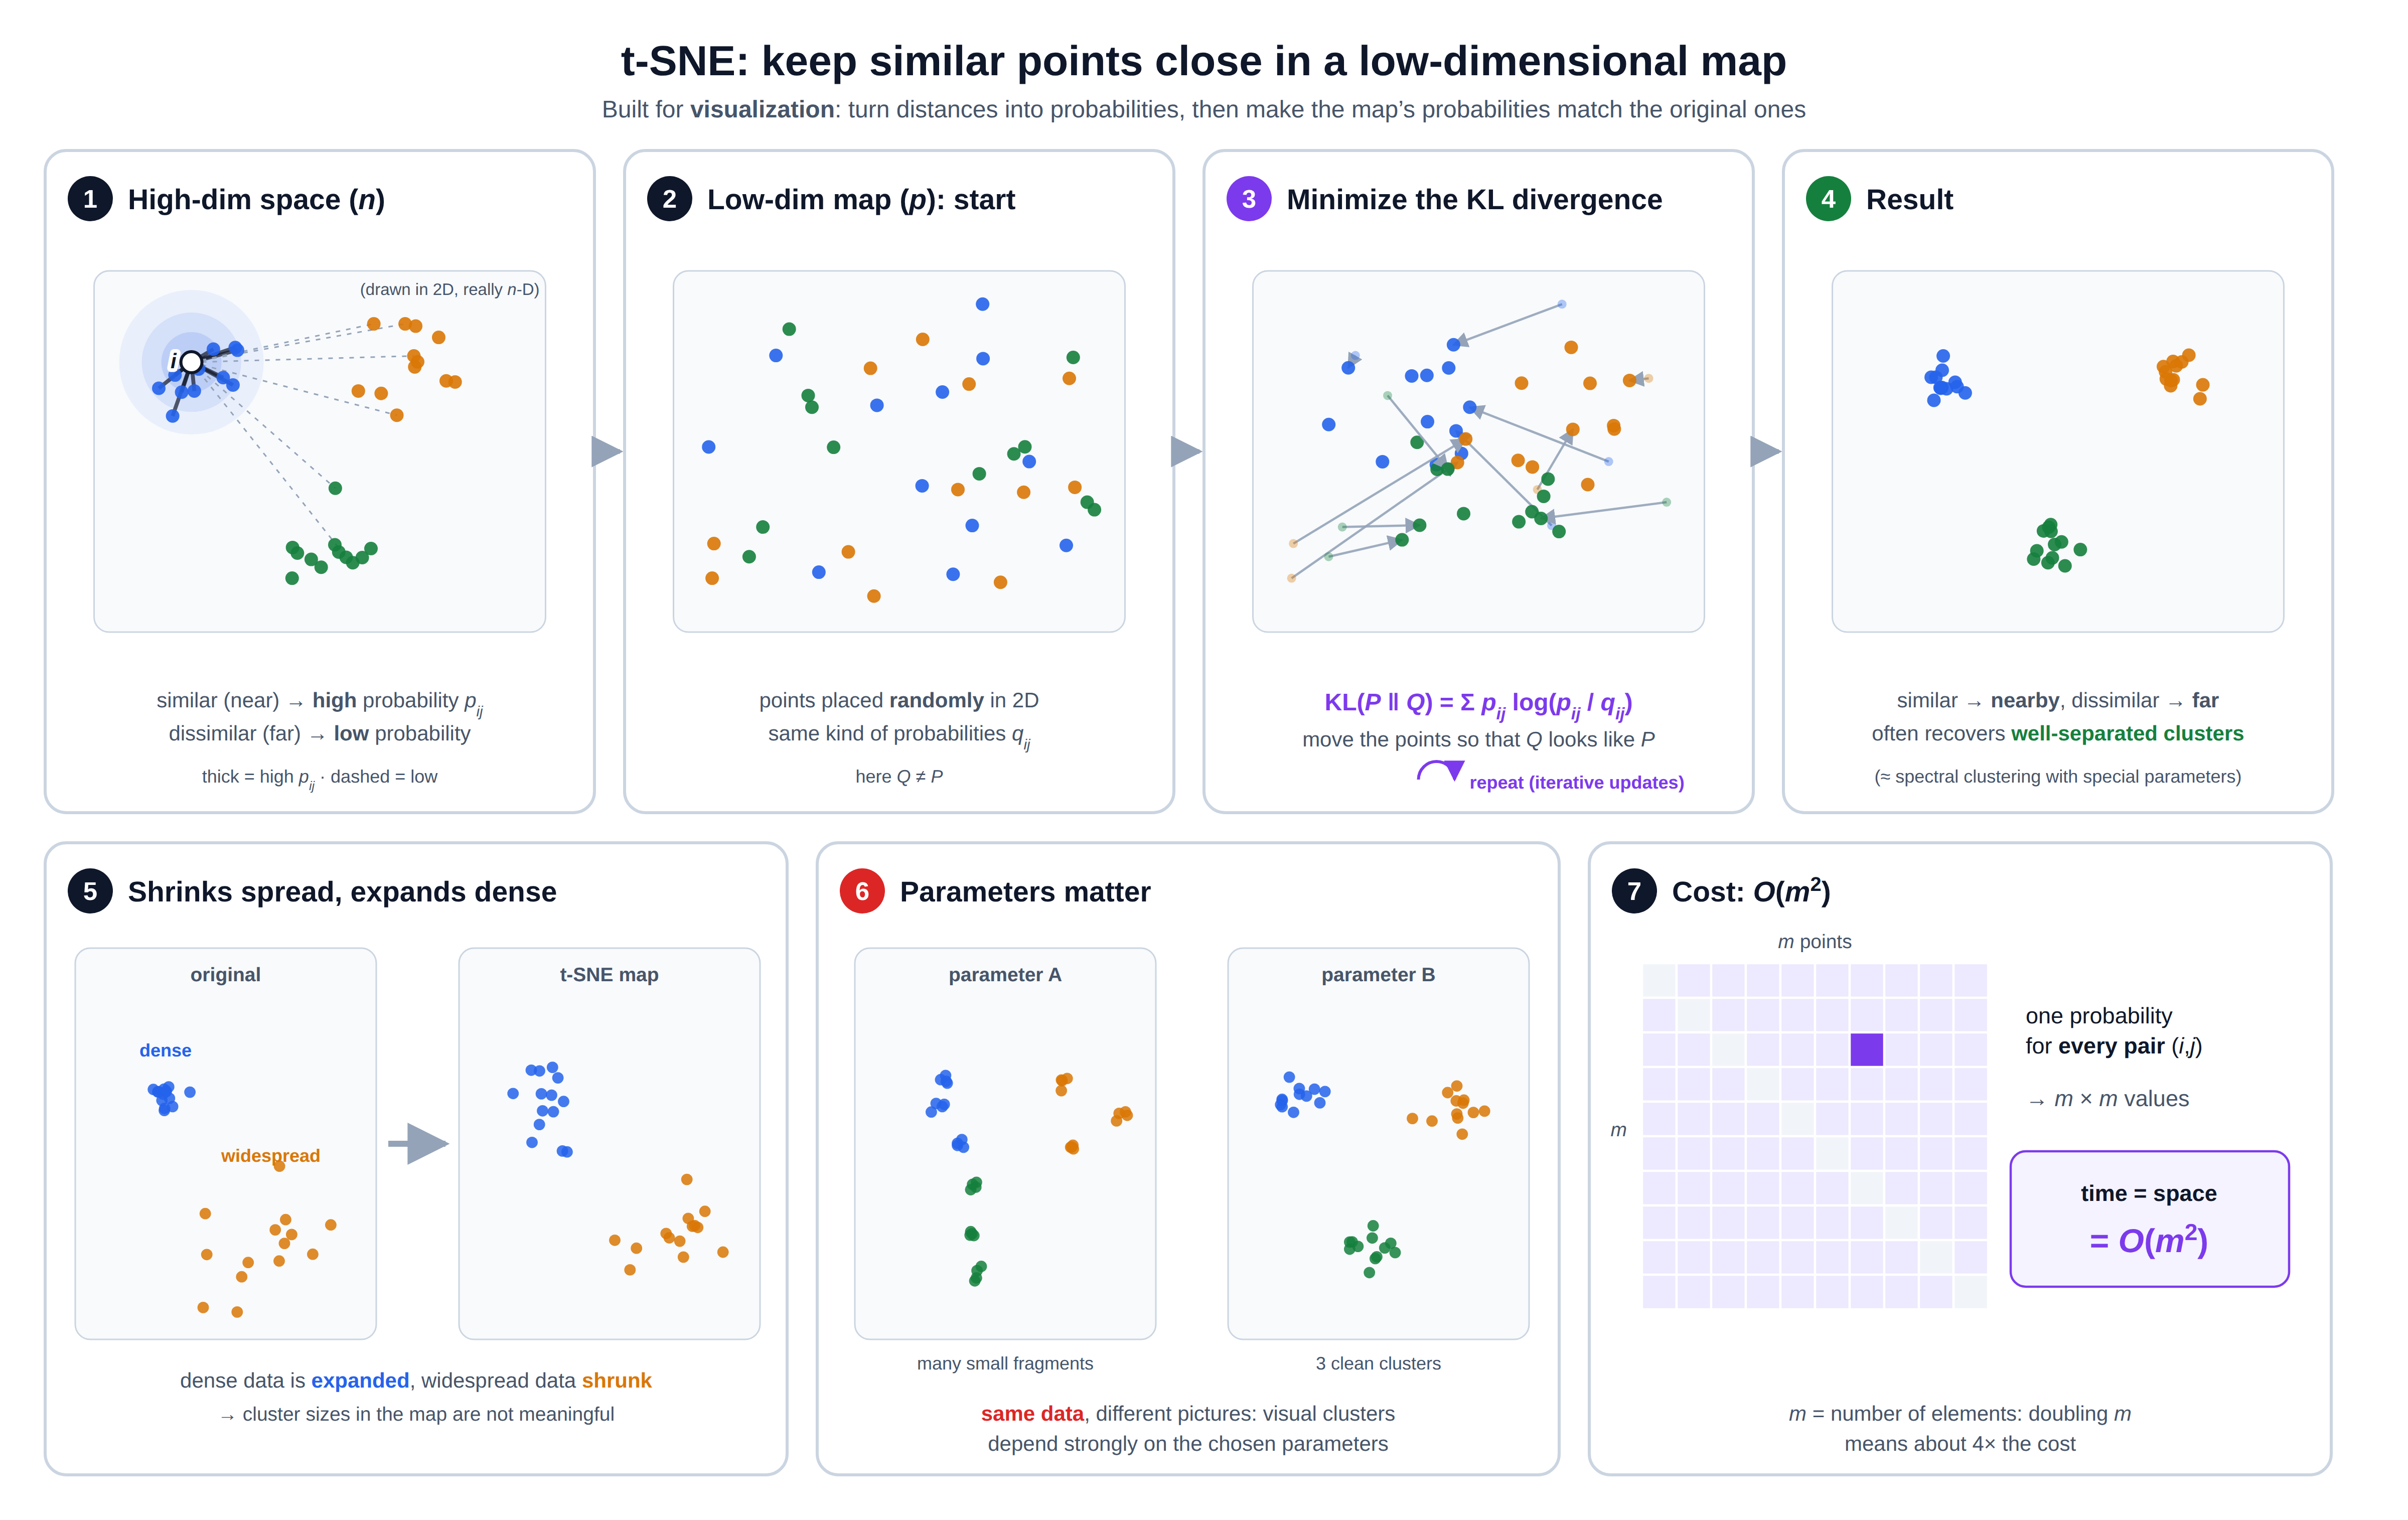
\includegraphics[width=0.5\textwidth]{images/chapter_4/tsne.png}
    \caption{t-SNE: from pairwise probabilities to a low-dimensional map}
\end{figure}

t-SNE works in 2 stages:

\begin{enumerate}
    \item In the \textbf{high-dimensional space} ($n$), build a probability distribution over pairs of objects. Similar objects get a high probability and dissimilar ones a low probability.
    \item In the \textbf{low-dimensional map} ($p$), define a similar probability distribution over the corresponding points.
\end{enumerate}

The low-dimensional map is then \textbf{iteratively updated} to minimize the \textbf{Kullback--Leibler divergence} between the two distributions. The goal is to make the $n$-space and $p$-space distributions as similar as possible.

Behaviour of t-SNE:
\begin{itemize}
    \item It \textbf{shrinks widespread data} and \textbf{expands densely packed data}.
    \item It often recovers \textbf{well-separated clusters}; with special parameter choices, it approximates a simple form of spectral clustering.
    \item The visual clusters can be \textbf{strongly influenced by the chosen parameters}.
\end{itemize}

Both its time and space complexity, with $m$ the number of elements, are:
\[
    \text{Complexity}_{\text{t-SNE}} = O(m^2)
\]

\subsection{PCA vs t-SNE}

\begin{itemize}
    \item \textbf{Distances}: t-SNE preserves \textbf{small pairwise distances} (local structure). PCA preserves \textbf{large pairwise distances} (global structure), in order to maximize the variance.
    \item \textbf{What is preserved}: PCA preserves the \textbf{variance} of the data. t-SNE preserves the \textbf{relationships between data points} in the lower-dimensional space, which makes it well suited to visualizing complex high-dimensional data.
\end{itemize}

\begin{figure}[h!]
    \centering
    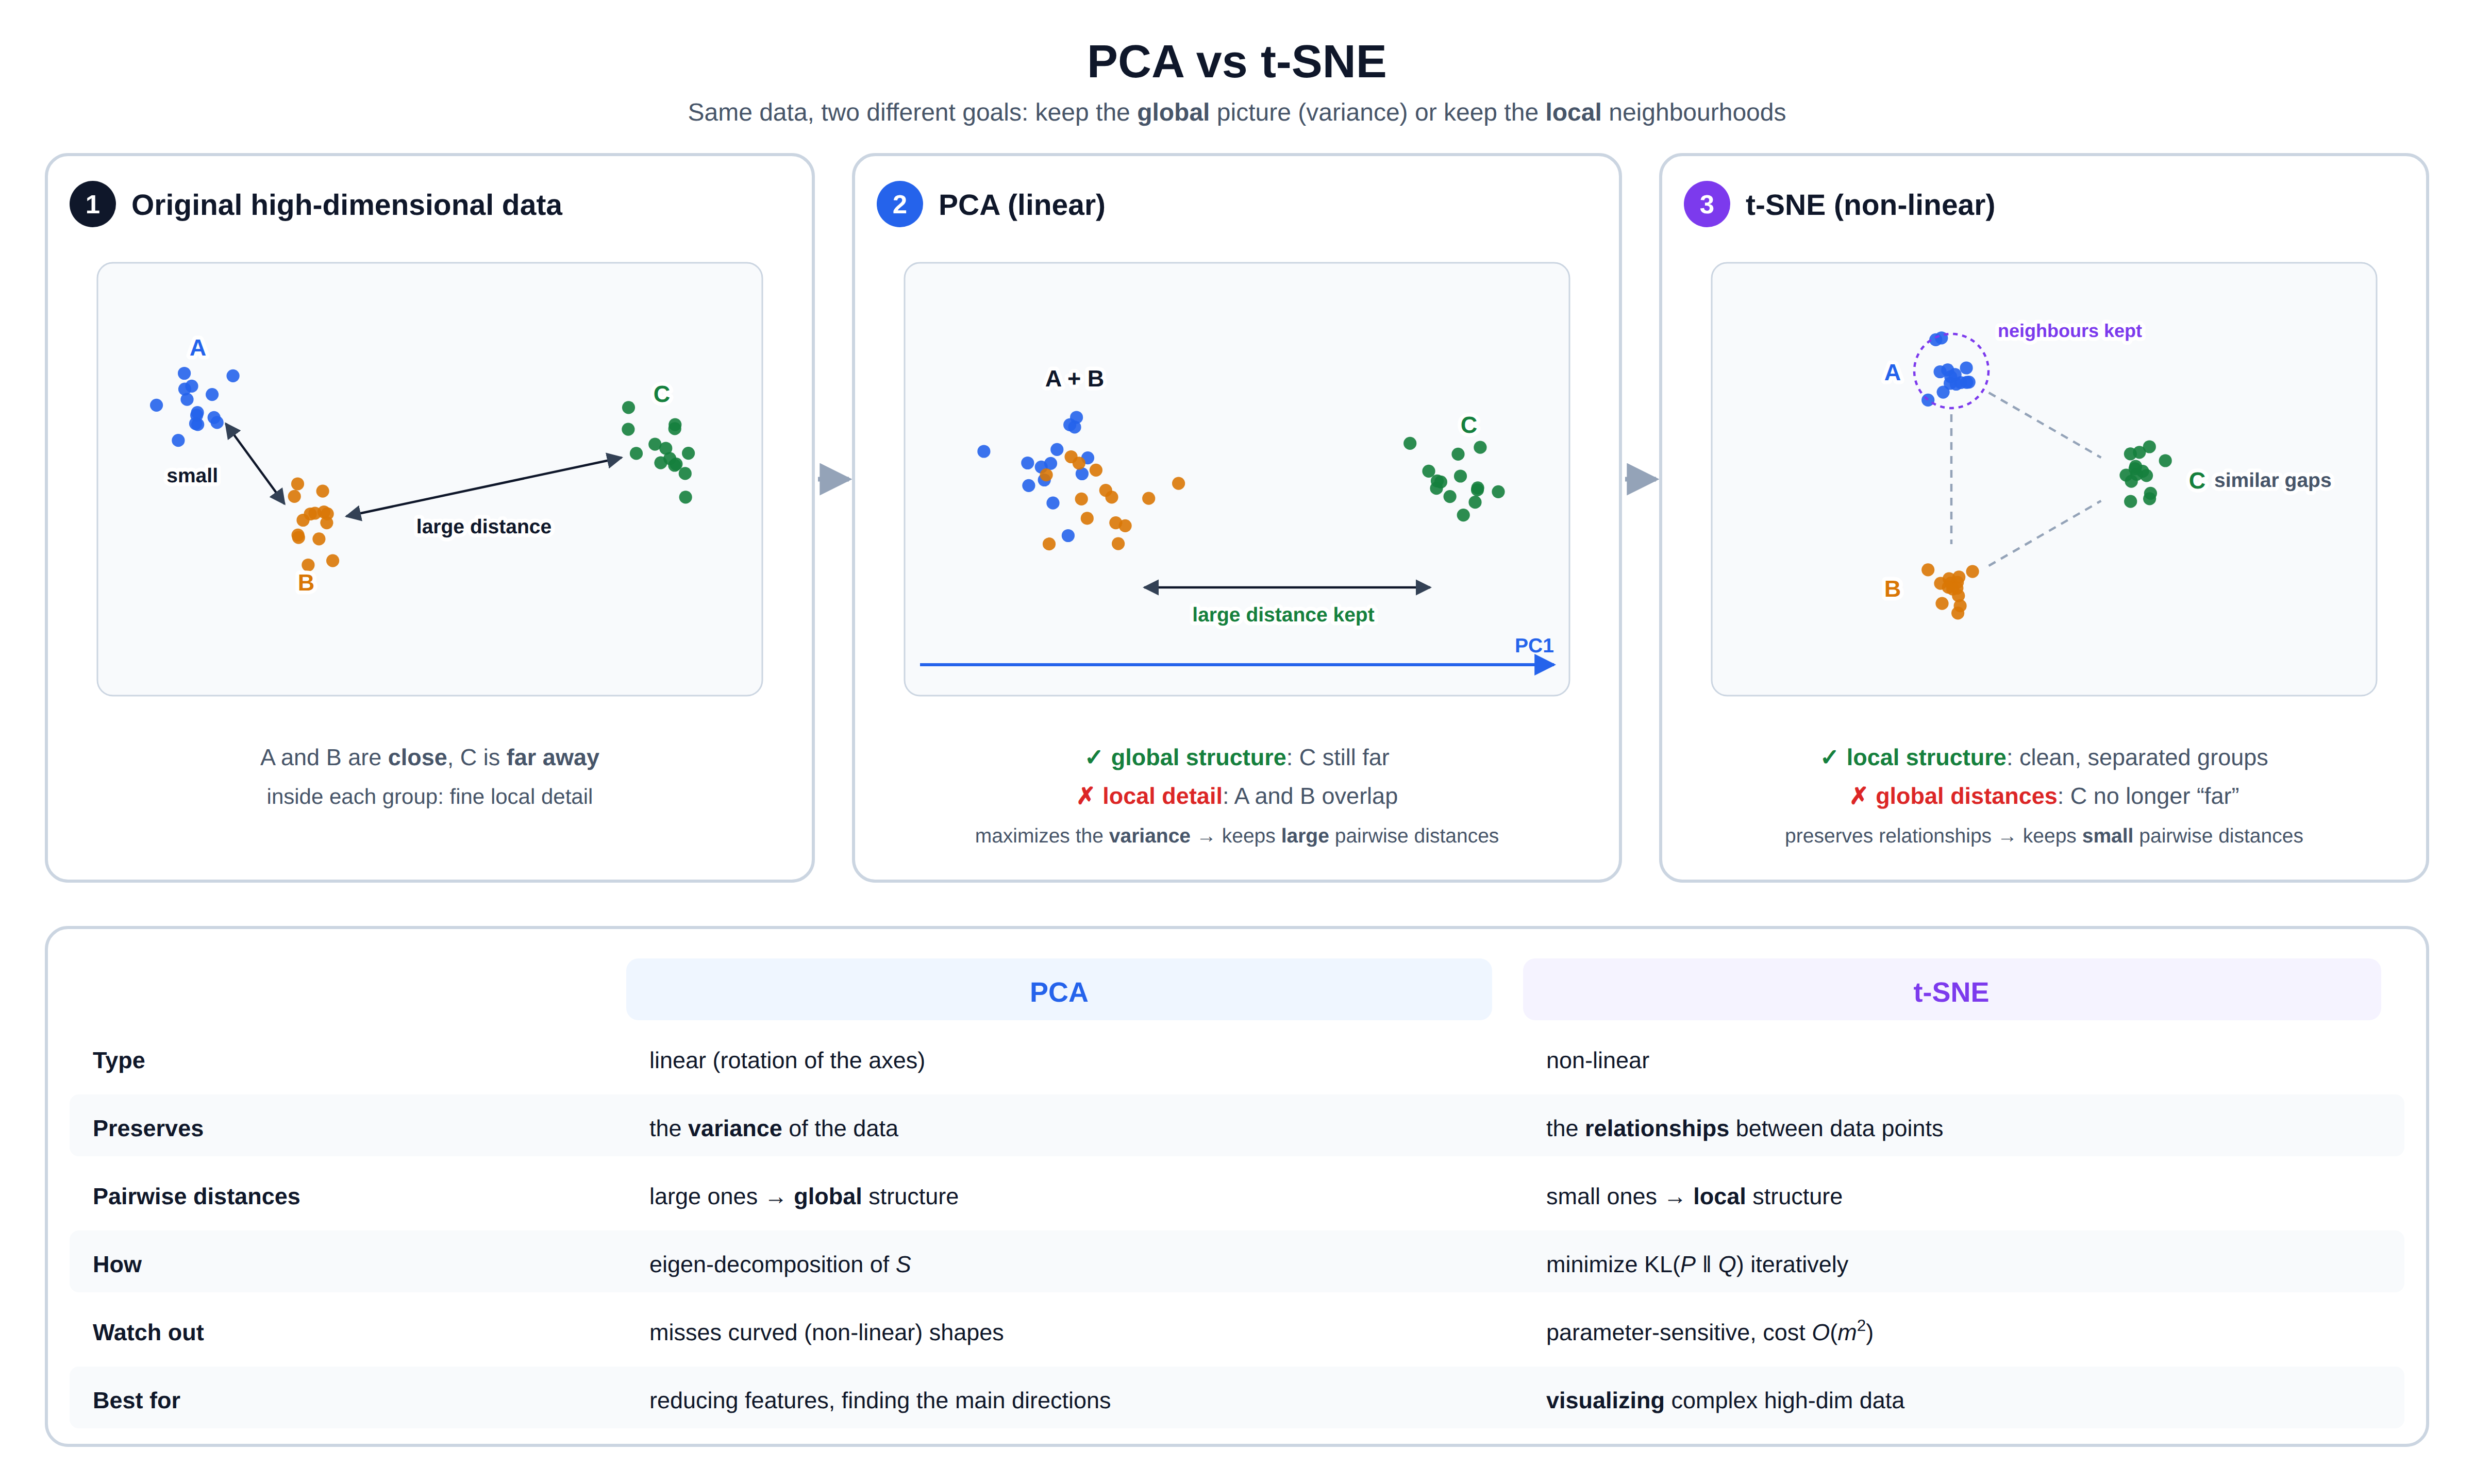
\includegraphics[width=1\textwidth]{images/chapter_4/pca_vs_tsne.png}
    \caption{PCA vs t-SNE: global vs local structure}
\end{figure}

\begin{figure}[h!]
    \centering
    \begin{minipage}{0.75\textwidth}
    \begin{itemize}
        \item Consider the following 5 samples with 4 features. Compute the principal components and their explained variance.
        \item For eigenvalues and eigenvectors, you can use Python (note: \texttt{eig} returns the eigenvectors as \emph{columns}):\\
        \texttt{from numpy.linalg import eig}\\
        \texttt{eigenvalues, eigenvectors = eig(A)}
    \end{itemize}

    \vspace{0.3cm}
    \centering
    \begin{tabular}{cccc}
        \toprule
        f1 & f2 & f3 & f4 \\
        \midrule
        1 & 2 & 3 & 4 \\
        5 & 5 & 6 & 7 \\
        1 & 4 & 2 & 3 \\
        5 & 3 & 2 & 1 \\
        8 & 1 & 2 & 2 \\
        \bottomrule
    \end{tabular}
    \end{minipage}
    \caption{Self-Assessment Quiz Chapter 4}
\end{figure}


\section{A prova di coglione}

\paragraph*{Il problema e l'idea.}
Quando i dati hanno molte dimensioni diventano difficili da visualizzare e da analizzare: è la \textbf{maledizione della dimensionalità}. La \textbf{Dimensionality Reduction} risolve il problema \emph{cambiando punto di vista}. I dati vengono descritti con \textbf{meno feature} ($p < n$), conservando l'informazione importante ed eliminando ridondanza e rumore. Lo schema è sempre lo stesso:
\begin{itemize}
    \item una funzione $h$ \textbf{comprime} il dato da $n$ a $p$ feature;
    \item una funzione $g$ lo \textbf{ricostruisce}, ottenendo $x' \approx x$;
    \item l'obiettivo è comprimere il più possibile con il minimo errore di ricostruzione.
\end{itemize}
I vantaggi sono modelli più leggeri e veloci, meno overfitting, meno rumore e dati visualizzabili.

\paragraph*{PCA: l'intuizione.}
La PCA è una \textbf{rotazione degli assi}. Si cerca un nuovo sistema di riferimento ortogonale in cui:
\begin{itemize}
    \item il \textbf{primo asse} segue la direzione di \textbf{massima varianza} dei dati;
    \item il secondo segue la massima varianza residua, ortogonale al primo, e così via.
\end{itemize}
Le nuove variabili, le \textbf{componenti principali}, sono combinazioni lineari di quelle originali e sono \textbf{scorrelate} tra loro. Se le variabili originali sono ridondanti (correlate), poche componenti bastano a spiegare quasi tutta la varianza. Massimizzare la varianza proiettata equivale a minimizzare l'errore di proiezione, cioè di ricostruzione: sono due facce dello stesso problema.

\paragraph*{PCA: la matematica in una riga.}
Tutto ruota attorno alla \textbf{matrice di covarianza} $S$ dei dati centrati:
\begin{itemize}
    \item gli \textbf{autovettori} di $S$ sono le nuove direzioni (gli assi principali);
    \item gli \textbf{autovalori} sono le varianze lungo quelle direzioni.
\end{itemize}
Usando gli autovettori come righe di $P$, la proiezione $X' = XP^t$ ha covarianza \textbf{diagonale}: le nuove feature non sono correlate. La quota di varianza spiegata dalla componente $i$ è
\[
    V_i = 100\,\frac{\lambda_i}{\sum_j \lambda_j}.
\]

\paragraph*{PCA in pratica.}
\begin{enumerate}
    \item Centrare (meglio ancora, \textbf{standardizzare}) i dati.
    \item Calcolare la matrice di covarianza.
    \item Calcolarne autovalori e autovettori.
    \item Ordinarli per autovalore decrescente.
    \item Tenere i primi $p$ autovettori.
    \item Proiettare i dati su di essi.
\end{enumerate}

Per scegliere $p$ ci sono tre criteri:
\begin{itemize}
    \item \textbf{Kaiser}: tenere le componenti con autovalore $> 1$;
    \item \textbf{soglia di varianza cumulata}: tenere componenti finché si supera, ad esempio, l'80--90\%;
    \item \textbf{metodo del gomito}: fermarsi dove la curva degli autovalori piega.
\end{itemize}

La standardizzazione è importante perché la PCA è sensibile alla scala: una variabile con valori grandi dominerebbe la varianza.

\paragraph*{Quando la PCA non basta.}
La PCA trova solo \textbf{assi lineari}. Se la struttura dei dati è non lineare, ad esempio dati disposti a cerchio, servono altri metodi:
\begin{itemize}
    \item \textbf{Kernel PCA}: i dati vengono mappati in un nuovo spazio $f(x)$ dove la struttura diventa lineare, e lì si applica la PCA. Grazie al kernel $K(x,y) = f(x)^t f(y)$ non serve calcolare esplicitamente $f$. Il risultato sono componenti non lineari nello spazio originale.
    \item \textbf{t-SNE}: è pensato per la \textbf{visualizzazione}. Costruisce una distribuzione di probabilità di ``vicinanza'' tra le coppie di punti nello spazio originale e una analoga nella mappa a bassa dimensione. Poi modifica la mappa finché le due distribuzioni sono il più simili possibile (minimizzando la divergenza di Kullback--Leibler). Punti simili finiscono vicini e punti diversi lontani. Fa emergere bene i cluster, ma il risultato dipende molto dai parametri e il costo è $O(m^2)$.
\end{itemize}

\paragraph*{PCA vs t-SNE a colpo d'occhio.}
\begin{center}
    \begin{tabular}{p{0.28\textwidth}p{0.3\textwidth}p{0.3\textwidth}}
        \toprule
        & \textbf{PCA} & \textbf{t-SNE} \\
        \midrule
        Tipo & Lineare & Non lineare \\
        Cosa preserva & Varianza, distanze grandi (struttura globale) & Vicinanze, distanze piccole (struttura locale) \\
        Uso tipico & Ridurre le feature, preprocessing & Visualizzare dati complessi, cluster \\
        Risultato & Deterministico, interpretabile & Dipende dai parametri \\
        \bottomrule
    \end{tabular}
\end{center}

\paragraph*{Da ricordare.}
\begin{itemize}
    \item Ridurre le dimensioni significa \textbf{comprimere senza perdere ciò che conta}.
    \item Nella PCA, ciò che conta è la \textbf{varianza}. Le componenti principali sono gli autovettori della covarianza, ordinati per autovalore.
    \item Le componenti principali sono \textbf{lineari, ortogonali e scorrelate}, e le prime spiegano la maggior parte della varianza.
    \item Quando i dati hanno strutture non lineari si usano Kernel PCA oppure t-SNE, quest'ultimo soprattutto per visualizzare.
\end{itemize}
%\chapter{The 3 components of ML}

Every Machine Learning method, from linear regression to deep neural networks, is built from the same three components:
\begin{itemize}
    \item \textbf{Data}: \emph{what do we learn from?}
    \item \textbf{Model}: \emph{which predictors are we allowed to use?}
    \item \textbf{Loss}: \emph{how do we measure if a predictor is good?}
\end{itemize}

\section{Data}

\textit{``For a lot of problems, we should shift our mindset toward not just improving the code but in a more systematic way of improving the data''.}

Data is a set of \textbf{data points} (also called samples, records or objects). Each data point carries two kinds of information:

\begin{itemize}
    \item \textbf{Features} $x$: \textbf{low-level} properties that are \textbf{easy to measure}. They are mainly numeric and are stacked into a \textbf{feature vector} $x = (x_1, \dots, x_n)$.
    \item \textbf{Label} $y$: the \textbf{high-level quantity of interest}, often \textbf{difficult to determine} (it may require an expert, time or money). The label is a \textbf{design choice}: by choosing what the label is, we are defining the ML problem (the learning task).
\end{itemize}

\emph{Example}: a data point is a network flow. Its features are easy to measure (packet sizes, duration, number of packets, ports). Its label could be the application that generated it (e.g.\ video, VoIP, web), which cannot be read directly from the traffic.

The type of label determines the type of task:
\begin{itemize}
    \item \textbf{Categorical label} $\rightarrow$ \textbf{classification}. With 2 categories it is \emph{binary} classification (e.g.\ normal vs.\ attack); with more than 2 it is \emph{multi-class} classification (e.g.\ video vs.\ VoIP vs.\ web).
    \item \textbf{Numerical label} $\rightarrow$ \textbf{regression} (e.g.\ predicting the throughput of a link).
    \item If a data point has \textbf{more than one label}, the problem is \textbf{multi-label}, and it requires multi-task learning.
\end{itemize}

\begin{figure}[h]
    \centering
    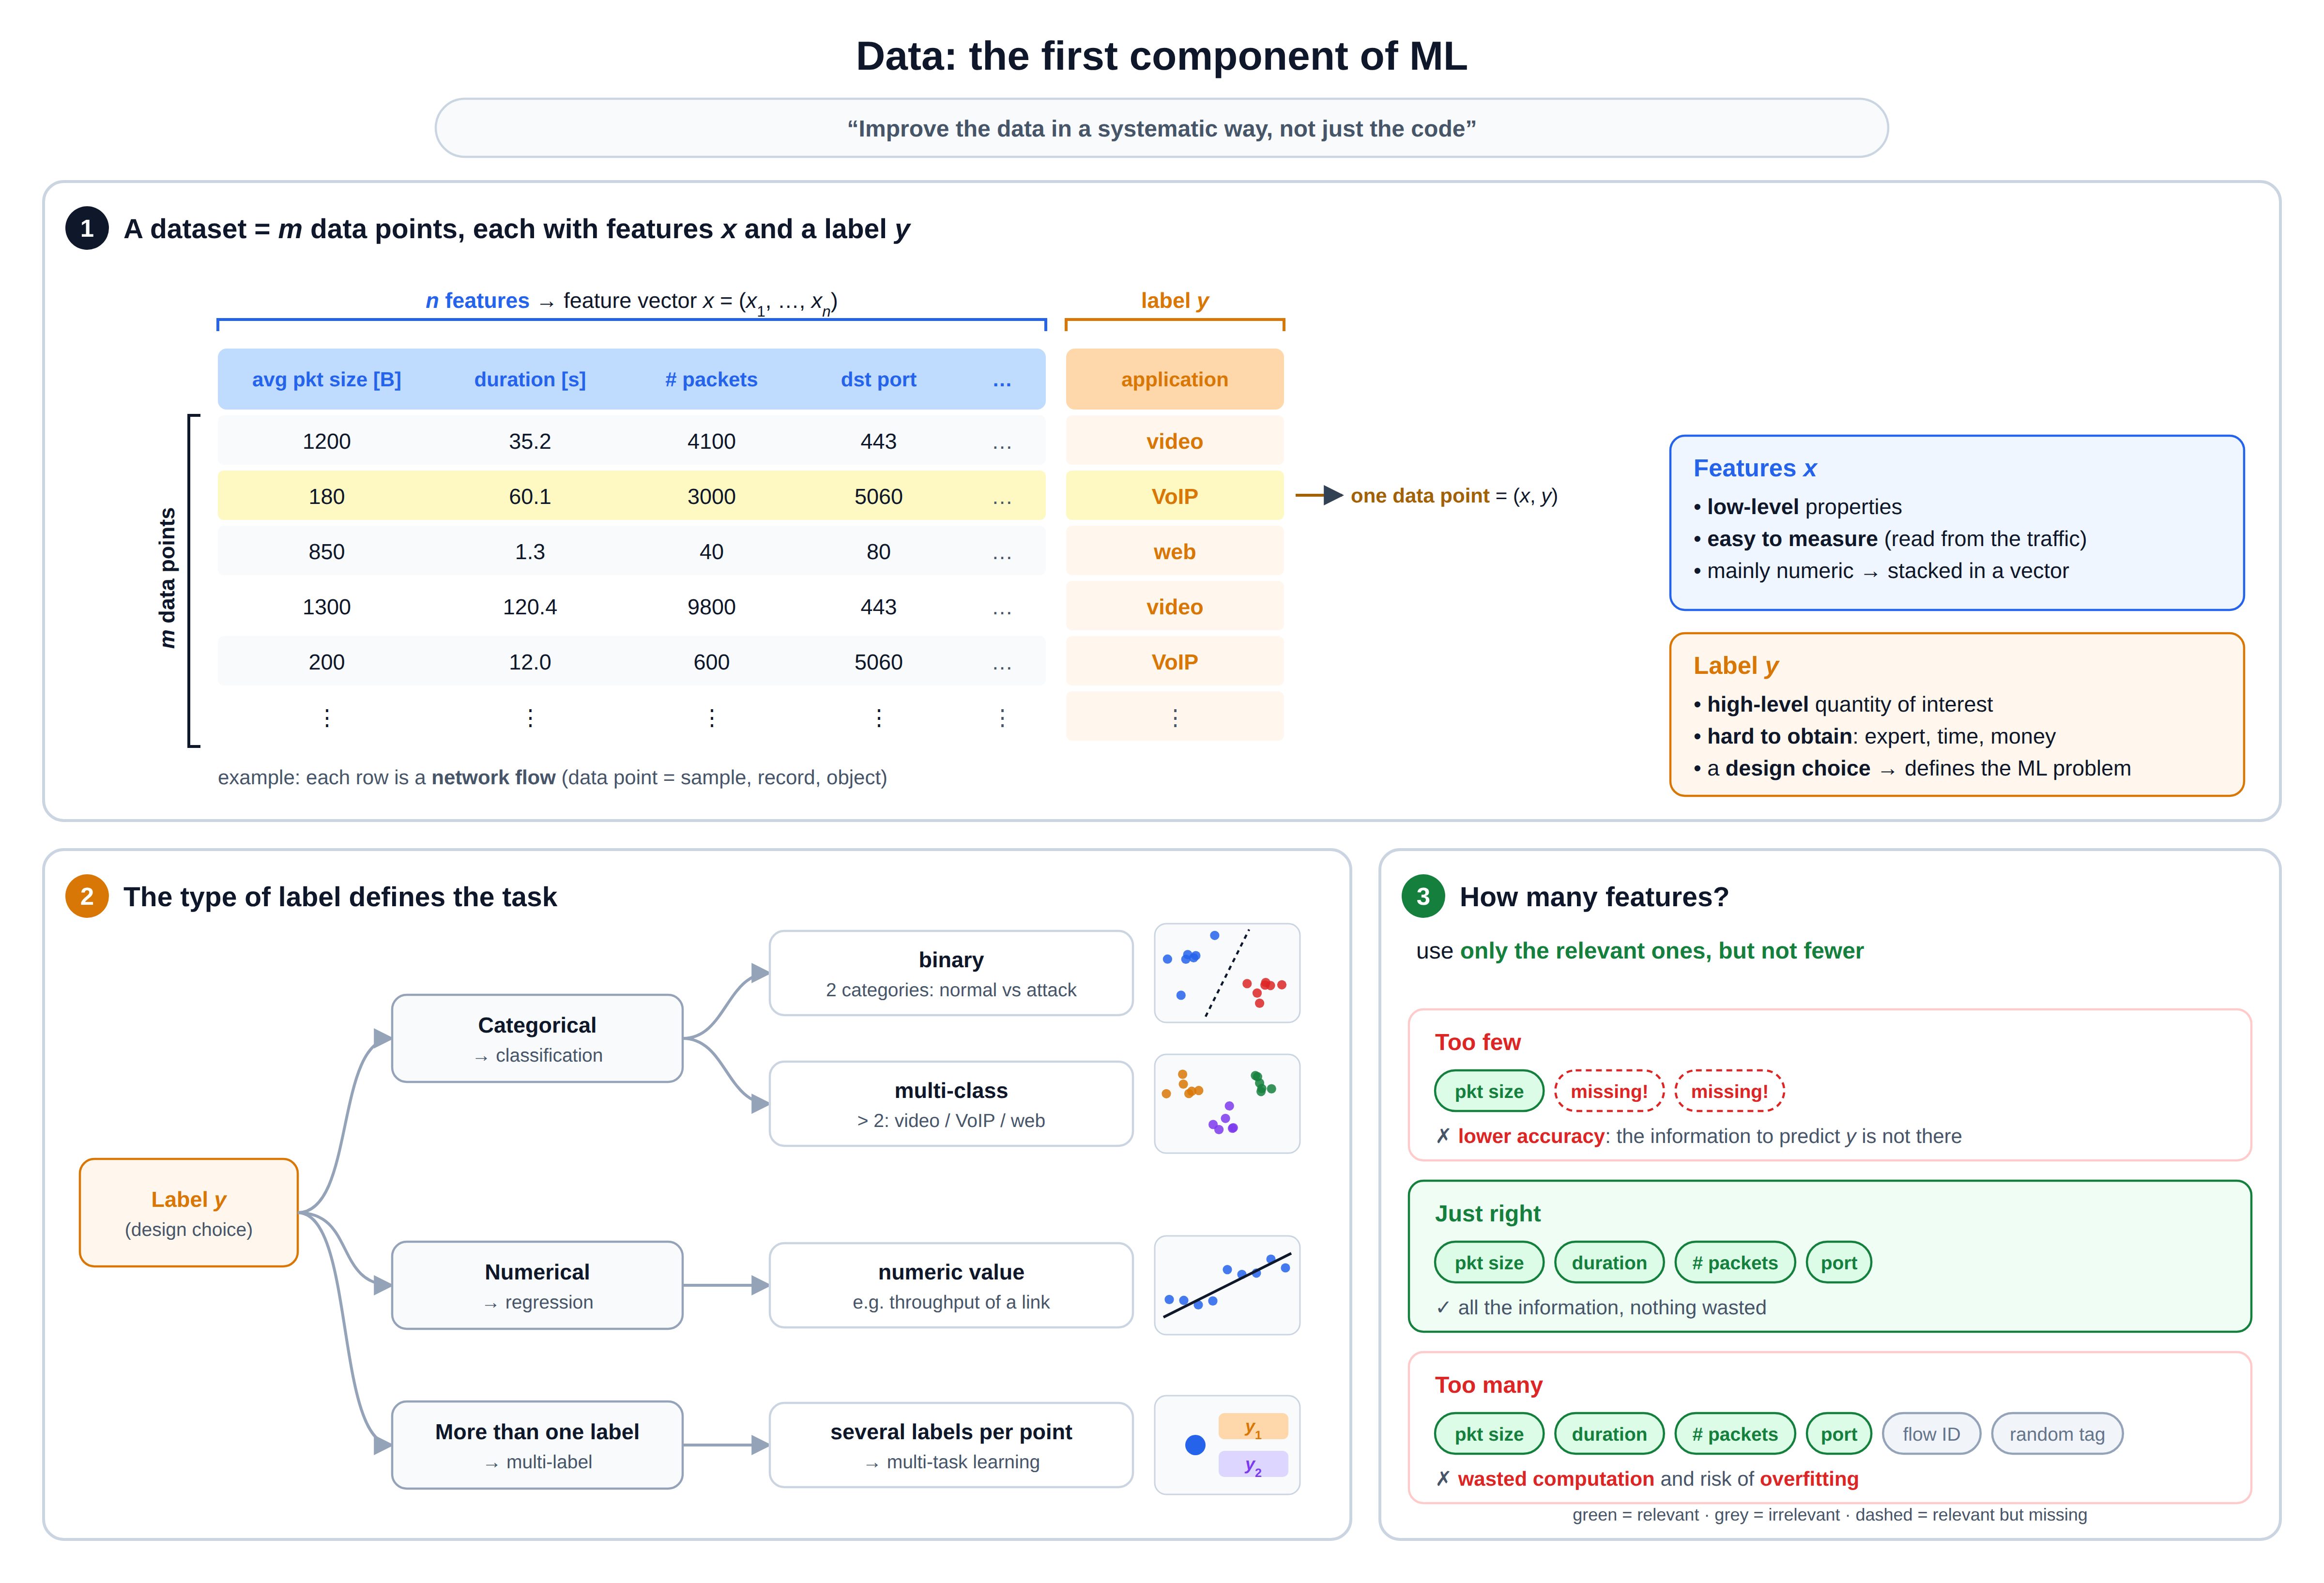
\includegraphics[width=1\textwidth]{images/chapter_5/ml_data.png}
    \caption{Data: data points, features and labels, the type of task, and how many features to use}
\end{figure}

\textbf{Notation}: $m$ is the number of data points, $n$ is the number of features.

\textbf{How many features?} Use \textbf{only the relevant ones, but not fewer}:
\begin{itemize}
    \item missing relevant features hurts \textbf{accuracy}, because the information needed to predict $y$ is not there;
    \item adding irrelevant features \textbf{wastes computation} and may cause \textbf{overfitting}.
\end{itemize}

\section{Model}
Every ML method aims at learning how to \textbf{predict the label $y$ of a data point from its features $x$}. In a nutshell, ML looks for a \textbf{hypothesis} (a predictor map) $h$ such that
\[
    h(x) \approx y
\]
The hypothesis is chosen from a set of candidates $\mathcal{H}$, called the \textbf{hypothesis space}; this set is what we call the \textbf{model}. Different ML methods use different hypothesis spaces: linear maps, polynomials, decision trees, artificial neural networks, and many others. The best hypothesis found during training is then used to find patterns, make predictions or classify new data.

\subsection{Size of the hypothesis space}
The hypothesis space $\mathcal{H}$ is a subset of $\mathcal{Y}^{\mathcal{X}}$, the set of \emph{all} possible maps from the feature space $\mathcal{X}$ to the label space $\mathcal{Y}$. Choosing $\mathcal{H}$ means choosing how large this subset is, and it must be:

\begin{itemize}
    \item \textbf{Large enough} to contain at least one good hypothesis. If $\mathcal{H}$ only contains straight lines but the true relation is curved, no $h$ will ever fit well.
    \item \textbf{Small enough}:
    \begin{itemize}
        \item to fit the \textbf{computational resources} available for learning (fitting) and training;
        \item to avoid \textbf{overfitting}: an analysis that corresponds too closely or exactly to a particular set of data, and may therefore fail to fit additional data. A very large $\mathcal{H}$ can ``memorize'' the training data instead of learning the general pattern.
    \end{itemize}
\end{itemize}

\begin{figure}[h]
    \centering
    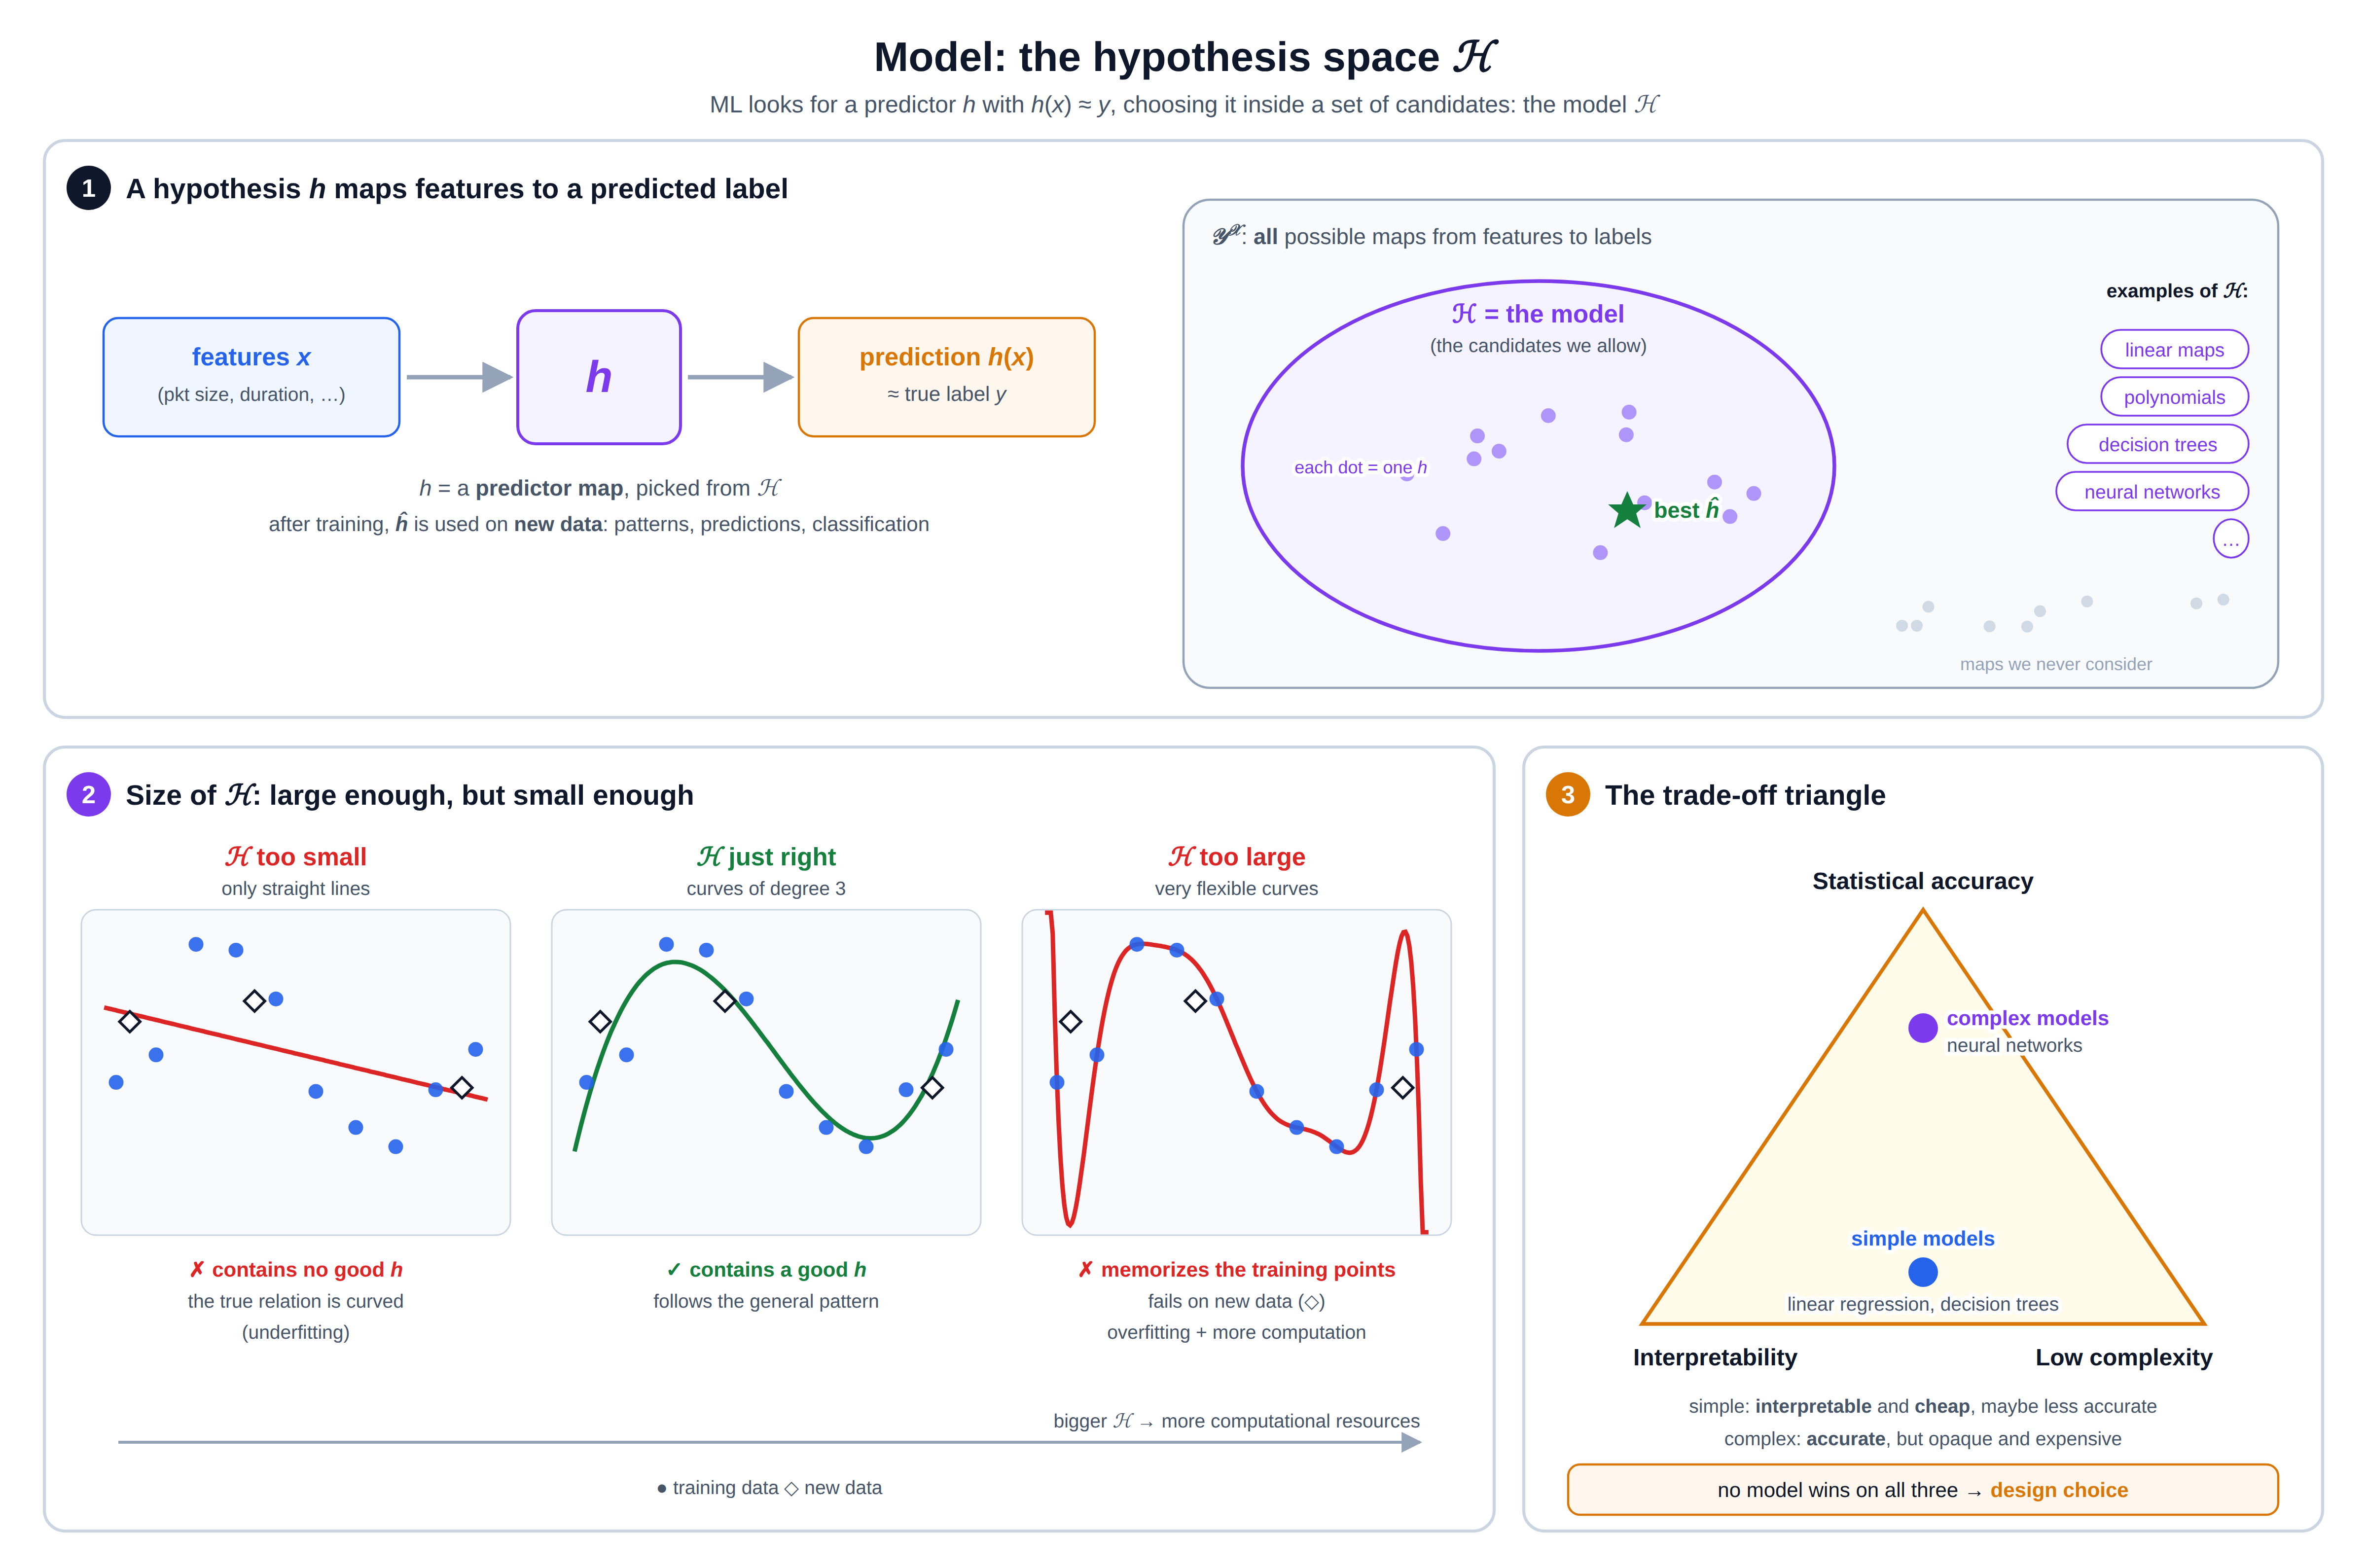
\includegraphics[width=1\textwidth]{images/chapter_5/ml_model.png}
    \caption{Model: the hypothesis space, its size and the trade-off triangle}
\end{figure}

When choosing $\mathcal{H}$ we must balance three competing aspects:
\begin{itemize}
    \item \textbf{Interpretability}: how easily we can understand and explain how the model makes predictions.
    \item \textbf{Statistical accuracy}: how accurate the predictions are.
    \item \textbf{Computational complexity}: the resources needed to train and deploy the model.
\end{itemize}

\textbf{Simple models} (linear regression, decision trees) are interpretable and computationally cheap, but may not reach high accuracy. \textbf{Complex models} (neural networks) can reach high accuracy, but they are harder to interpret and more expensive. There is no universal best choice: finding the right balance in this triangle is a \textbf{design choice}.

\section{Loss}

To decide which hypothesis $h \in \mathcal{H}$ to pick, we need a way to tell good predictors from bad ones. A \textbf{loss function} $L((x,y),h)$ is a quantitative measure of the \textbf{prediction error} we make when we use $h(x)$ to predict the true label $y$ of a data point: the smaller the loss, the better the prediction. Common examples are:
\begin{itemize}
    \item \textbf{Squared error loss}: $L = (y - h(x))^2$, which penalizes large errors heavily;
    \item \textbf{Absolute error loss}: $L = |y - h(x)|$, which is more robust to outliers.
\end{itemize}

\begin{figure}[h]
    \centering
    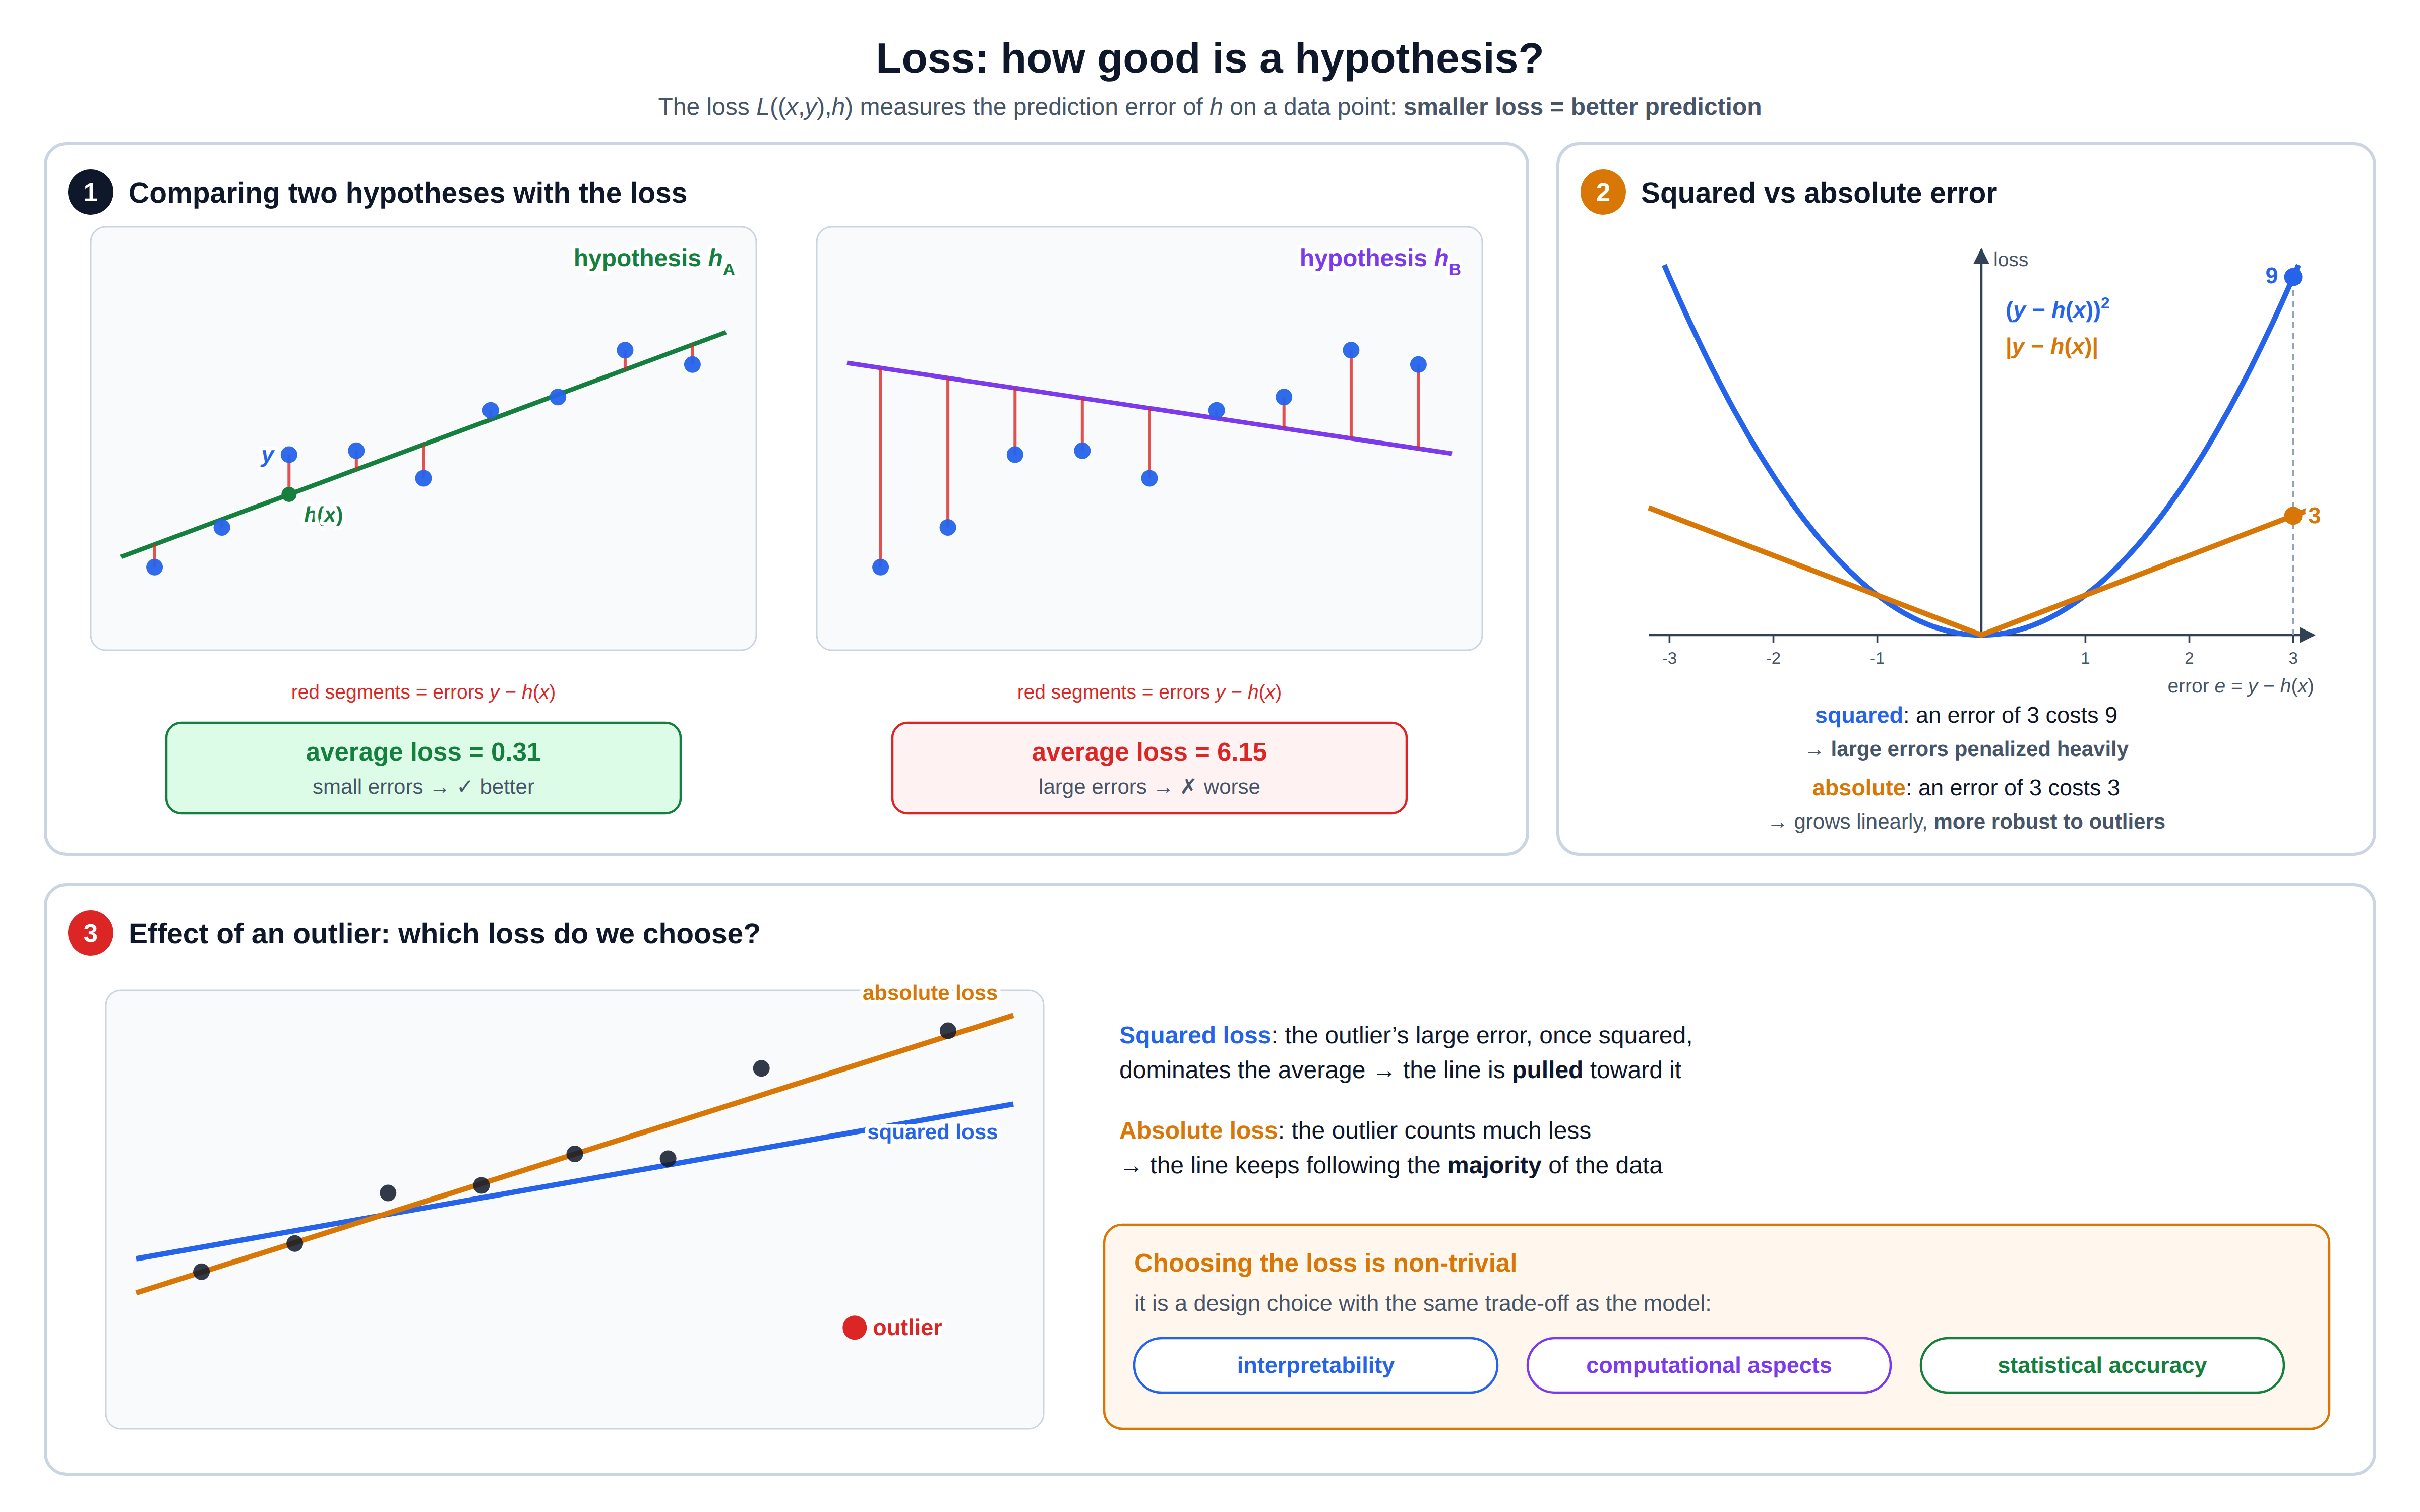
\includegraphics[width=1\textwidth]{images/chapter_5/ml_loss.png}
    \caption{Loss: comparing hypotheses, squared vs absolute error, effect of an outlier}
\end{figure}

Choosing a suitable loss is often non-trivial. Like the model, it involves the trade-off between interpretability, computational aspects and statistical accuracy.

\section{Putting the 3 components together}

Learning means using the \textbf{data} to pick, from the \textbf{model} $\mathcal{H}$, the hypothesis with the smallest \textbf{loss}, on average over the $m$ data points:
\[
    \hat{h} = \arg\min_{h \in \mathcal{H}} \; \frac{1}{m} \sum_{i=1}^{m} L\big((x^{(i)}, y^{(i)}),\, h\big)
\]
The chosen $\hat{h}$ is then used to predict the labels of \textbf{new} data points, for which only the features are known.

Each component also reflects a step of the scientific method:
\begin{itemize}
    \item the \textbf{data} are the \emph{observations};
    \item the \textbf{model} contains the \emph{hypotheses} that try to explain them;
    \item the \textbf{loss} \emph{validates} each hypothesis against the observations, so that we can make accurate predictions and inference on additional observations.
\end{itemize}

\begin{figure}[h]
    \centering
    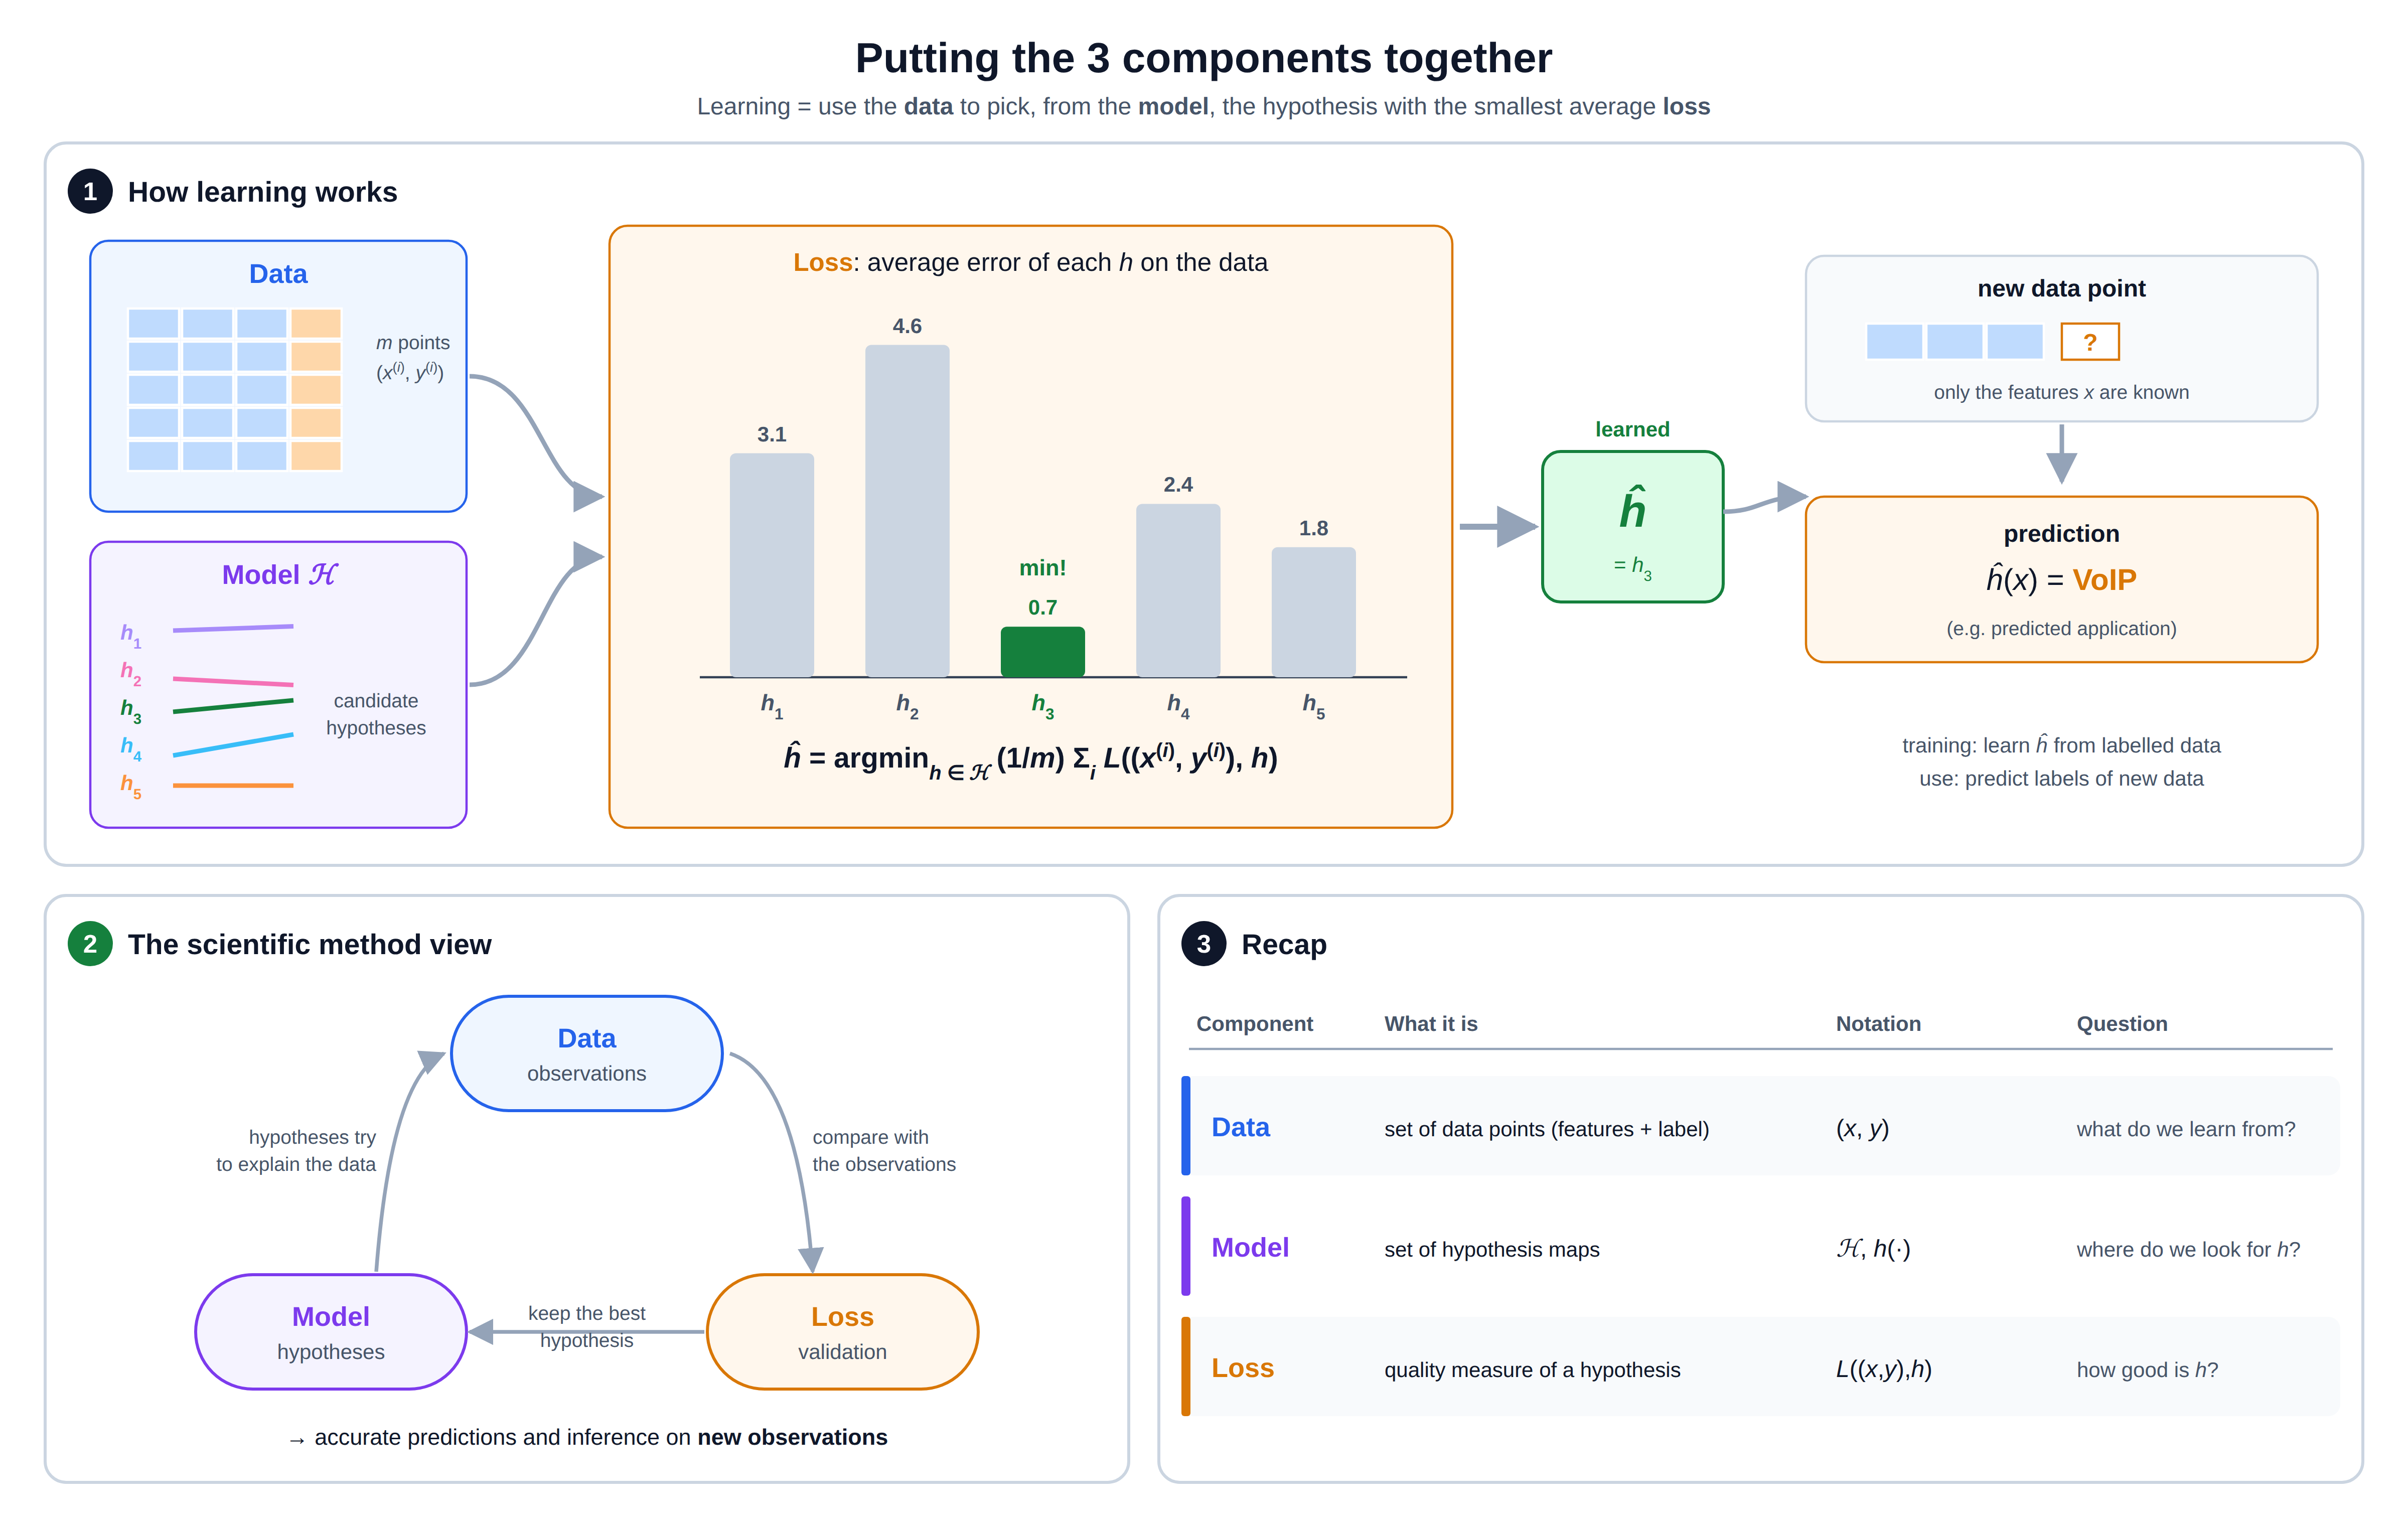
\includegraphics[width=1\textwidth]{images/chapter_5/ml_three_components.png}
    \caption{How data, model and loss work together}
\end{figure}

\begin{center}
    \begin{tabular}{lll}
        \toprule
        \textbf{Component} & \textbf{What it is} & \textbf{Notation} \\
        \midrule
        Data  & set of data points (features + label) & $(x, y)$ \\
        Model & set of hypothesis maps                & $\mathcal{H}$, \ $h(\cdot)$ \\
        Loss  & quality measure of a hypothesis       & $L((x, y), h)$ \\
        \bottomrule
    \end{tabular}
\end{center}


\section{A prova di coglione}

\paragraph*{L'idea di fondo.}
Qualsiasi metodo di Machine Learning, dalla regressione lineare alle reti neurali profonde, nasce dalla combinazione di tre ingredienti: i \textbf{dati}, il \textbf{modello} e la \textbf{loss}. Cambiano i dettagli, ma lo schema è sempre lo stesso. Abbiamo degli esempi da cui imparare, un insieme di possibili ``regole'' tra cui scegliere e un criterio per giudicare quale regola funziona meglio. Capire questi tre elementi significa capire la struttura di ogni algoritmo di ML.

\paragraph*{I dati: da cosa impariamo.}
I dati sono un insieme di $m$ \textbf{data point}, cioè gli esempi. Ognuno porta con sé due tipi di informazione:
\begin{itemize}
    \item le \textbf{feature} $x$: proprietà facili da misurare, raccolte in un vettore di $n$ numeri;
    \item la \textbf{label} $y$: la grandezza che ci interessa davvero, ma che è difficile o costosa da ottenere.
\end{itemize}
In una rete, ad esempio, di un flusso di traffico misuriamo facilmente dimensioni dei pacchetti e durata (le feature), ma vorremmo sapere quale applicazione lo ha generato (la label). Il punto chiave è che \textbf{scegliere la label significa scegliere il problema}:
\begin{itemize}
    \item label a categorie $\rightarrow$ classificazione (binaria o multi-classe);
    \item label numerica $\rightarrow$ regressione;
    \item più label per lo stesso data point $\rightarrow$ problema multi-label.
\end{itemize}
Anche le feature vanno scelte con cura: servono quelle rilevanti, né di più né di meno. Se ne mancano alcune, l'informazione per predire $y$ non c'è. Se ce ne sono troppe inutili, si spreca calcolo e si rischia l'overfitting.

\paragraph*{Il modello: dove cerchiamo la soluzione.}
L'obiettivo del ML è trovare una funzione, l'\textbf{ipotesi} $h$, che a partire dalle feature restituisca una buona stima della label: $h(x) \approx y$. Non la cerchiamo tra tutte le funzioni possibili, ma dentro un insieme scelto da noi, lo \textbf{spazio delle ipotesi} $\mathcal{H}$, che è ciò che chiamiamo \emph{modello}. Scegliere di usare ``solo rette'', ``solo alberi di decisione'' o ``reti neurali'' significa scegliere $\mathcal{H}$.

Quanto deve essere grande questo insieme?
\begin{itemize}
    \item \textbf{Abbastanza grande} da contenere una buona soluzione: se cerco solo tra le rette e il fenomeno è curvo, non la troverò mai.
    \item \textbf{Abbastanza piccolo} da essere gestibile con le risorse di calcolo, e soprattutto da evitare l'\textbf{overfitting}. Un modello troppo ricco può ``imparare a memoria'' i dati di training invece di coglierne lo schema generale, e poi sbaglia sui dati nuovi.
\end{itemize}
Nella scelta entra in gioco un \textbf{triangolo di compromessi} tra interpretabilità, accuratezza e costo computazionale:
\begin{itemize}
    \item i modelli semplici sono comprensibili ed economici, ma a volte poco precisi;
    \item i modelli complessi sono precisi, ma opachi e costosi.
\end{itemize}
Non esiste una scelta giusta in assoluto: è una decisione di progetto.

\paragraph*{La loss: come giudichiamo una soluzione.}
Dentro $\mathcal{H}$ ci sono moltissime ipotesi, e per sceglierne una serve un criterio numerico. La \textbf{loss} $L((x,y),h)$ misura quanto sbaglia l'ipotesi $h$ su un data point, confrontando la predizione $h(x)$ con la vera label $y$: più è bassa, meglio è. L'errore si può misurare in modi diversi:
\begin{itemize}
    \item l'\textbf{errore quadratico} punisce molto gli errori grandi;
    \item l'\textbf{errore assoluto} è più tollerante verso i valori anomali.
\end{itemize}
Anche questa scelta non è banale e risente dello stesso triangolo di compromessi.

\paragraph*{Il meccanismo: come i tre pezzi lavorano insieme.}
Imparare significa usare i \textbf{dati} per scegliere, tra tutte le ipotesi del \textbf{modello}, quella con la \textbf{loss} media più bassa sugli esempi disponibili:
\[
    \hat{h} = \arg\min_{h \in \mathcal{H}} \frac{1}{m}\sum_{i=1}^{m} L\big((x^{(i)},y^{(i)}),h\big)
\]
Una volta trovata, $\hat{h}$ viene usata su data point \textbf{nuovi}, di cui conosciamo solo le feature, per predirne la label.

È lo stesso ragionamento del metodo scientifico:
\begin{itemize}
    \item i dati sono le \emph{osservazioni};
    \item il modello contiene le \emph{ipotesi} che provano a spiegarle;
    \item la loss è la \emph{verifica} che ci dice quale ipotesi regge meglio il confronto con la realtà.
\end{itemize}

\paragraph*{Da ricordare.}
\begin{itemize}
    \item \textbf{Dati}: esempi $(x, y)$. Le feature si misurano facilmente, la label è ciò che vogliamo predire, e la sua scelta definisce il problema.
    \item \textbf{Modello}: l'insieme $\mathcal{H}$ in cui cerchiamo $h$. Né troppo piccolo (non contiene la soluzione) né troppo grande (overfitting, costi).
    \item \textbf{Loss}: il voto numerico che misura l'errore di $h$.
    \item \textbf{Apprendimento}: scegliere in $\mathcal{H}$ l'ipotesi che sui dati ha la loss media minima.
\end{itemize}
\chapter{Empirical Risk}
As we already stated, ML aims at learning a \textbf{hypothesis} $h$: a function that reads the \textbf{features} $x$ of a data point and returns a prediction of its \textbf{label} $y$. A \textbf{data point} $(x,y)$ is any object we are interested in. 

We want $h(x)$ to be close to $y$ not only for the data points we already have, but for \textbf{any data point we might encounter} in the future.\\

\begin{center}
    \textit{To reason about data we have not seen yet, we need a probabilistic model. Data points are interpreted as realizations of \textbf{random variables (RVs)}. A RV is a quantity whose value depends on the outcome of a random experiment, and a realization is the specific value we observe. These RVs are assumed to be \textbf{i.i.d.} (independent and identically distributed): data points do not influence each other (independent), and all of them are generated by the same \textbf{probability distribution} $p(x,y)$ (identically distributed). }
\end{center}

To measure how wrong a prediction is, we use a \textbf{loss function}, which assigns a non-negative number to each data point: the larger the loss, the worse the prediction $h(x)$ compared to the true label $y$. However, the loss on a single data point says little about $h$ in general. What we really care about is the \textbf{expected loss}, also called \textbf{expected risk}: the average loss of $h$ over all possible data points, where each point is weighted by how likely it is according to $p(x,y)$. A hypothesis with \textcolor{red}{small expected risk makes good predictions on future data}.\\

The problem is that computing the expected risk requires knowing $p(x,y)$, which in practice is never available. What we do have is a finite set of labelled data points, the \textbf{training set}. The idea is therefore to approximate the expected risk with the \textbf{empirical risk}, defined as the \textbf{average loss on the data points of the training set}. Since the training points are i.i.d. samples of $p(x,y)$, the empirical risk is a reasonable estimate of the expected risk. \textcolor{red}{This estimate becomes more accurate as the number of training points grows}.\\

\begin{figure}[h]
    \centering
    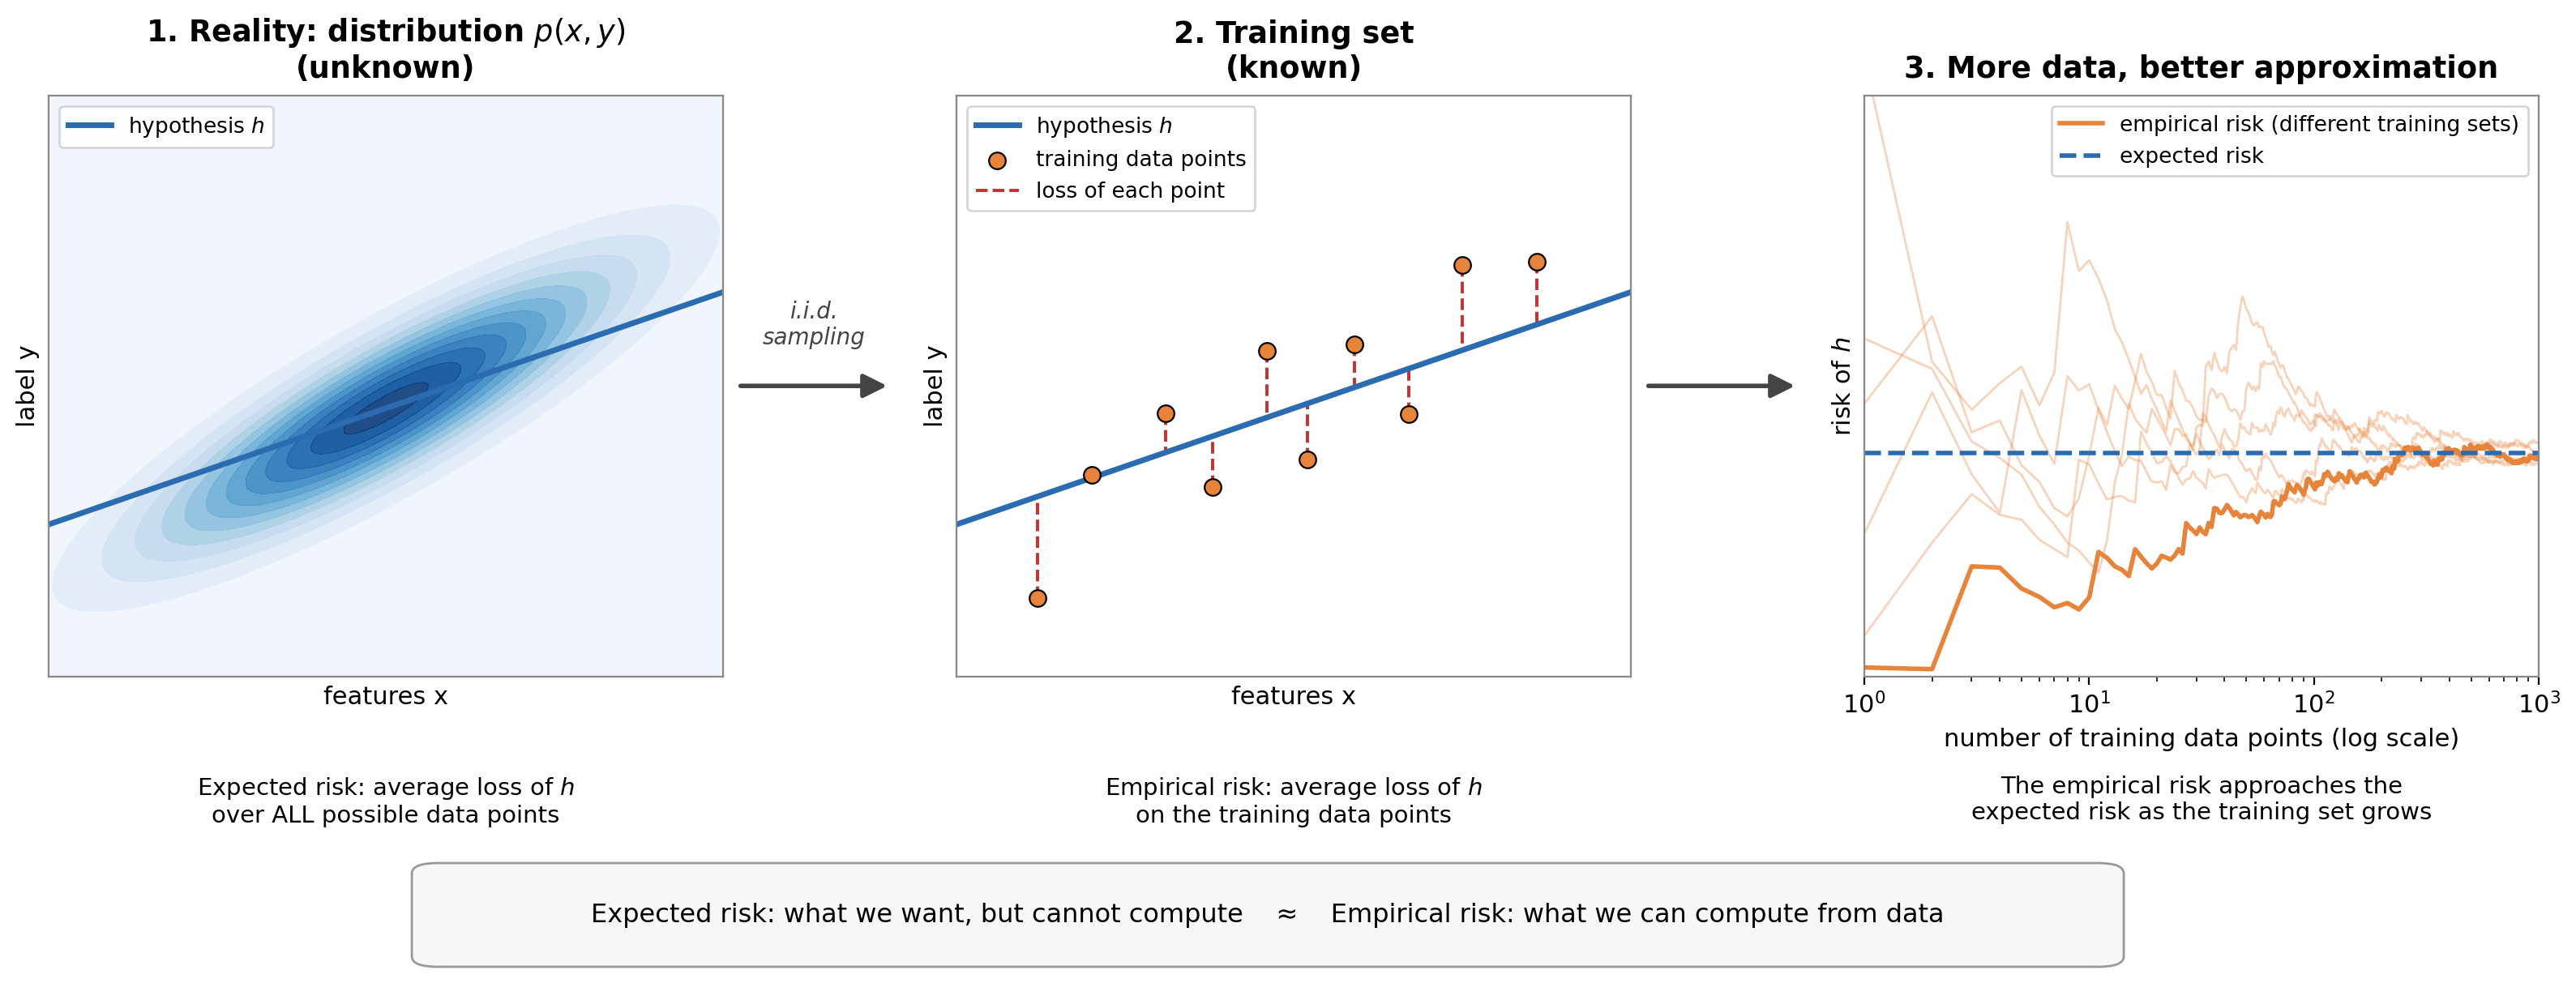
\includegraphics[width=1\textwidth]{images/chapter_6/ch_empirical_risk.png}
    \caption{From the unknown distribution $p(x,y)$ to the training set: the empirical risk approximates the expected risk, and the approximation improves as the training set grows.}
\end{figure}

In short, the expected risk is what we would like to minimize but cannot compute, while the empirical risk is what we can compute and use in its place.

\section{Empirical Risk Minimization}
\textbf{Empirical Risk Minimization} (ERM) turns the idea of the previous section into a learning principle. Among all hypotheses of the \textbf{hypothesis space} (the model), we choose the one with the \textbf{smallest empirical risk}, i.e. the one that makes the smallest average loss when predicting the \textbf{labels} of the training data points from their \textbf{features}.

When the hypotheses are described by a parameter vector (for instance the weights of a linear map), choosing the best hypothesis means choosing the best parameter vector. Learning therefore becomes an \textbf{optimization problem}: find the parameters that minimize the empirical risk.

It is important to keep in mind that ERM only looks at the training data. It works well as long as the empirical risk is a good approximation of the expected risk; when the two differ, the hypothesis that is best on the training set may not be the best on new data.

\begin{figure}[h]
    \centering
    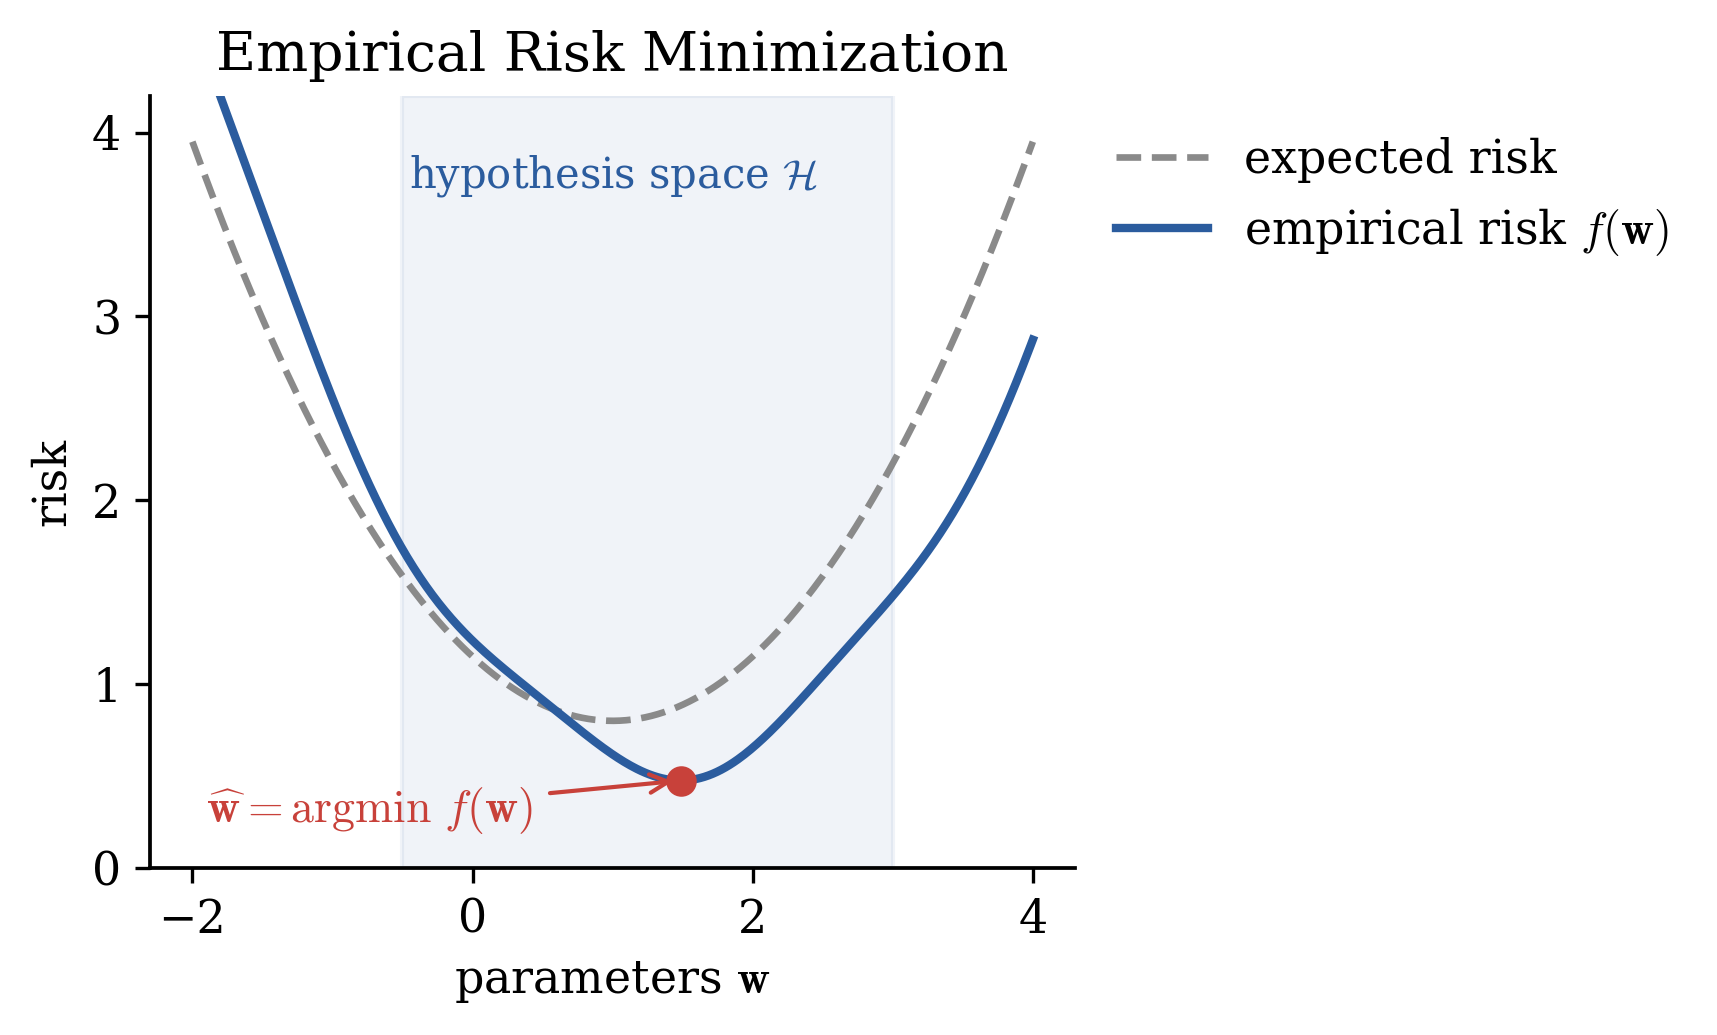
\includegraphics[width=0.8\textwidth]{images/chapter_6/sec_erm.png}
    \caption{Empirical risk vs expected risk and optimal parameter vector}
\end{figure}

\section{ERM for regression}
ERM can be applied to different kinds of problems, which mainly differ in the type of label:

\begin{itemize}
    \item \textbf{Regression}: the label is a \textbf{number} that can take continuous values (e.g. a price or a temperature). The loss measures the \textbf{distance} between the predicted number and the true one.
    \item \textbf{Classification}: the label is a \textbf{category}, chosen among two classes (binary) or more (multi-class). Since we cannot measure a ``distance'' between categories, the loss is based on how \textbf{confident} the prediction is and whether it is correct.
\end{itemize}

\begin{figure}[h]
    \centering
    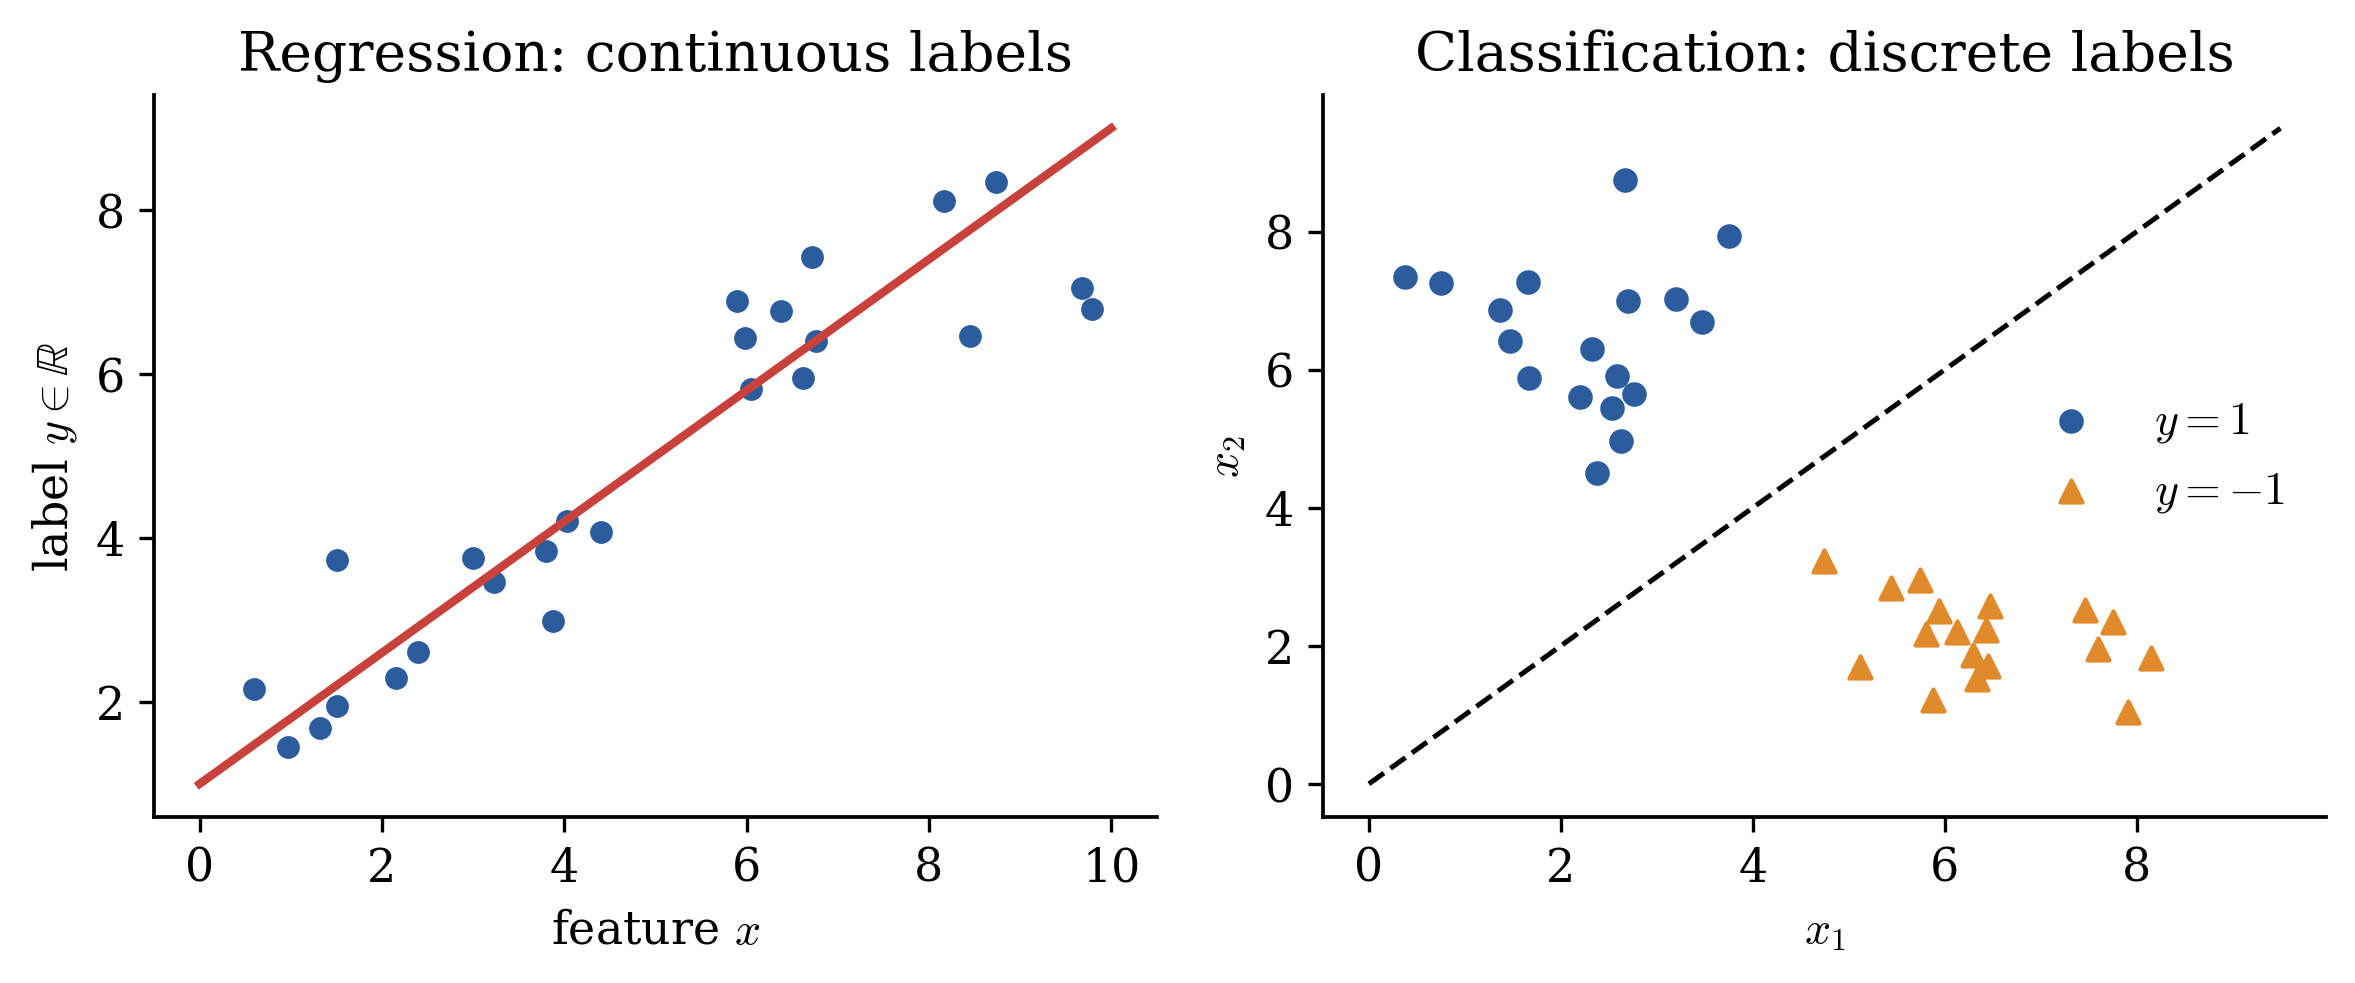
\includegraphics[width=0.9\textwidth]{images/chapter_6/sec_erm_regression.png}
    \caption{Regression vs Classification}
\end{figure}

\subsection{Linear Regression}
Linear regression is ERM with the following three choices:

\begin{itemize}
    \item \textbf{Data}: each data point has a \textbf{numeric feature vector} and a \textbf{numeric label}.
    \item \textbf{Model}: \textbf{linear hypothesis maps}, i.e. the prediction is a weighted sum of the features.
    \item \textbf{Loss}: \textbf{squared error loss}.
\end{itemize}

A straight line is often too simple to describe the data. \textbf{Polynomial Regression} solves this by first transforming the features into their powers ($x, x^2, \dots, x^n$) and then applying ordinary linear regression to these new features. The resulting hypothesis is a polynomial of degree $n$ in the original feature, but it is still \emph{linear in the parameters}. In other words, the model becomes larger and more flexible, while the method stays exactly the same.

\begin{figure}[h]
    \centering
    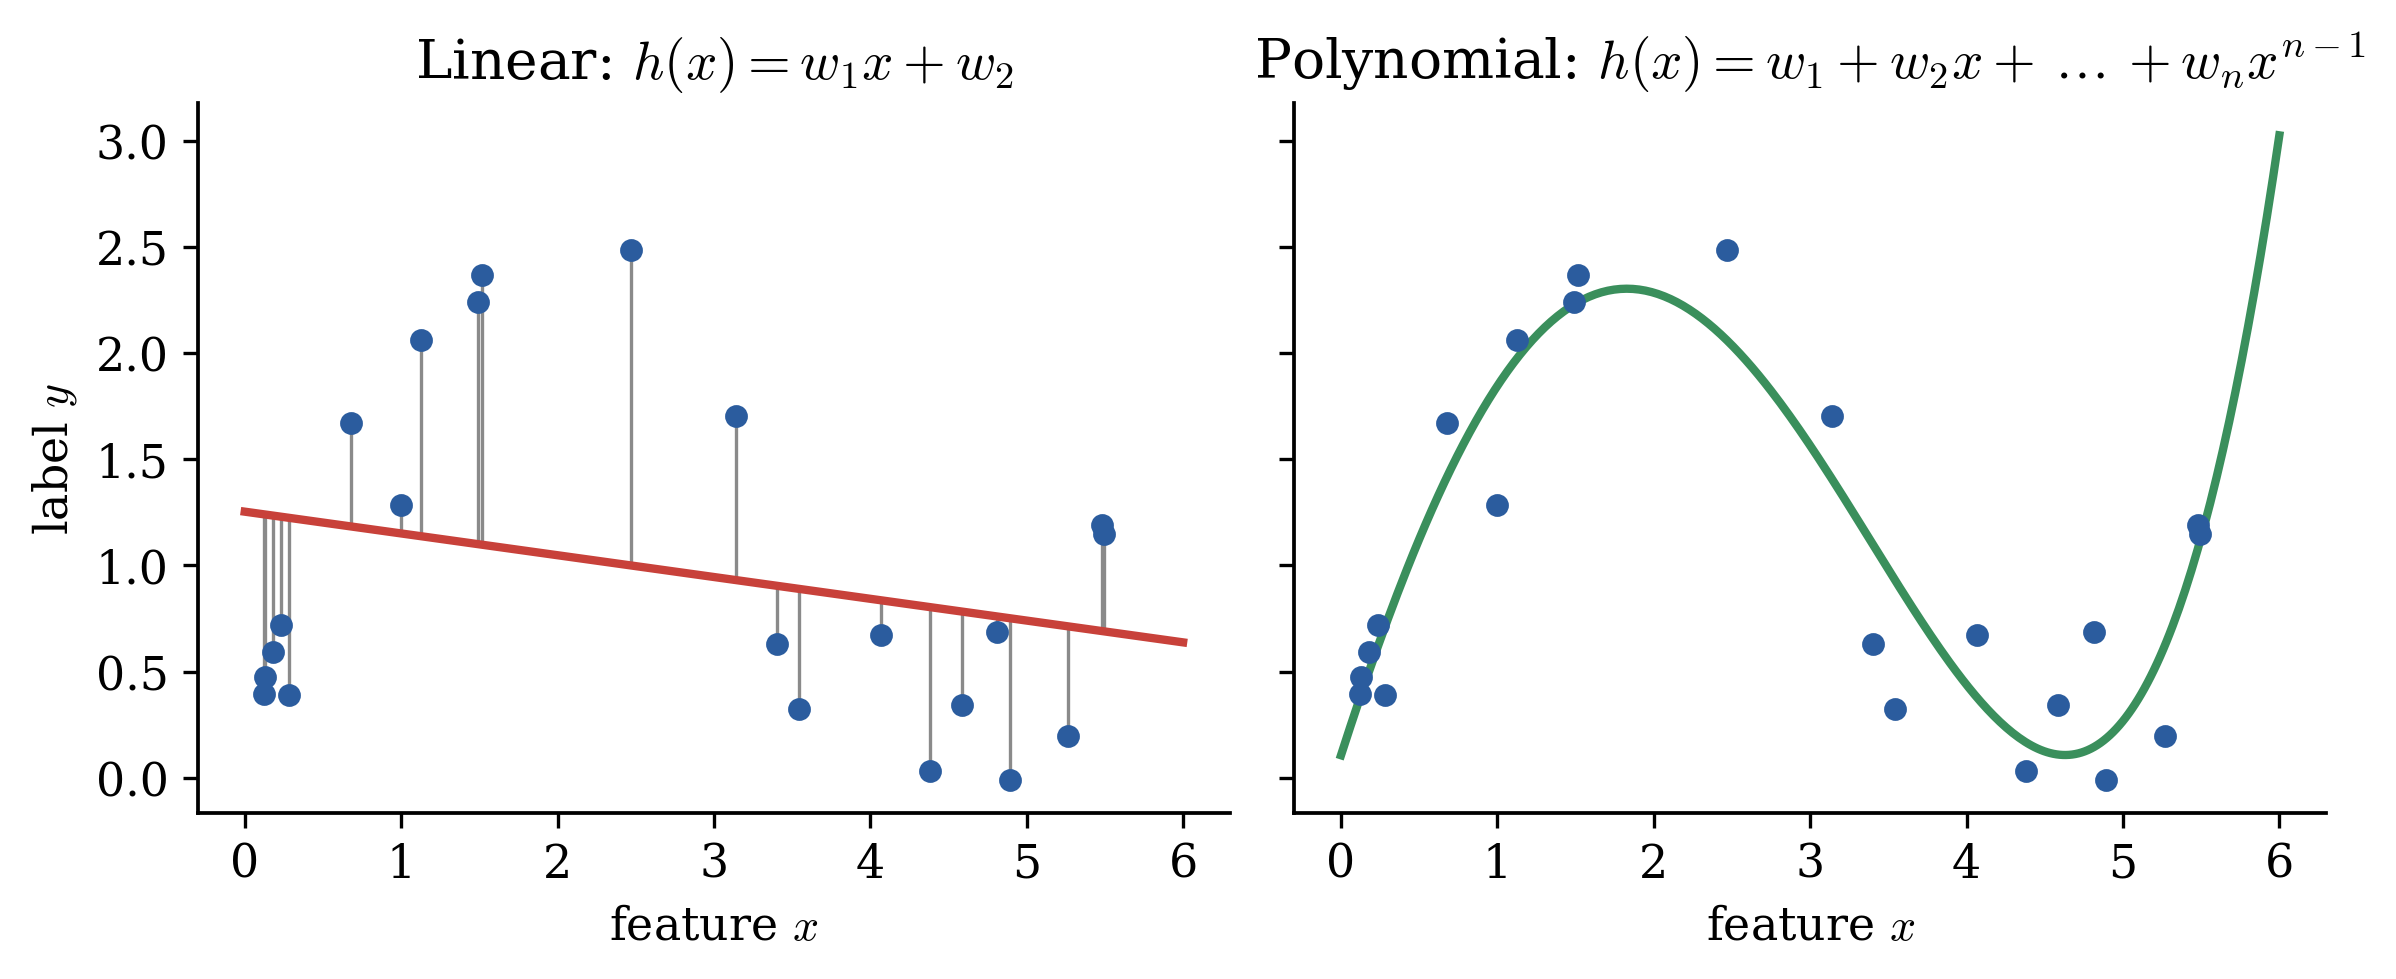
\includegraphics[width=0.9\textwidth]{images/chapter_6/sub_linear_regression.png}
    \caption{Linear Regression vs Polynomial Regression}
\end{figure}

\subsection{Loss Functions for regression}
The loss function decides \textbf{how much each error counts}. All regression losses are zero when the prediction is exact and grow as the prediction moves away from the true label; what changes is \textbf{how fast they grow}, and therefore how they treat large errors such as those caused by \textbf{outliers}. We consider three of them:

\begin{itemize}
    \item Squared Error Loss
    \item Absolute Error Loss
    \item Huber Loss
\end{itemize}

\begin{figure}[h]
    \centering
    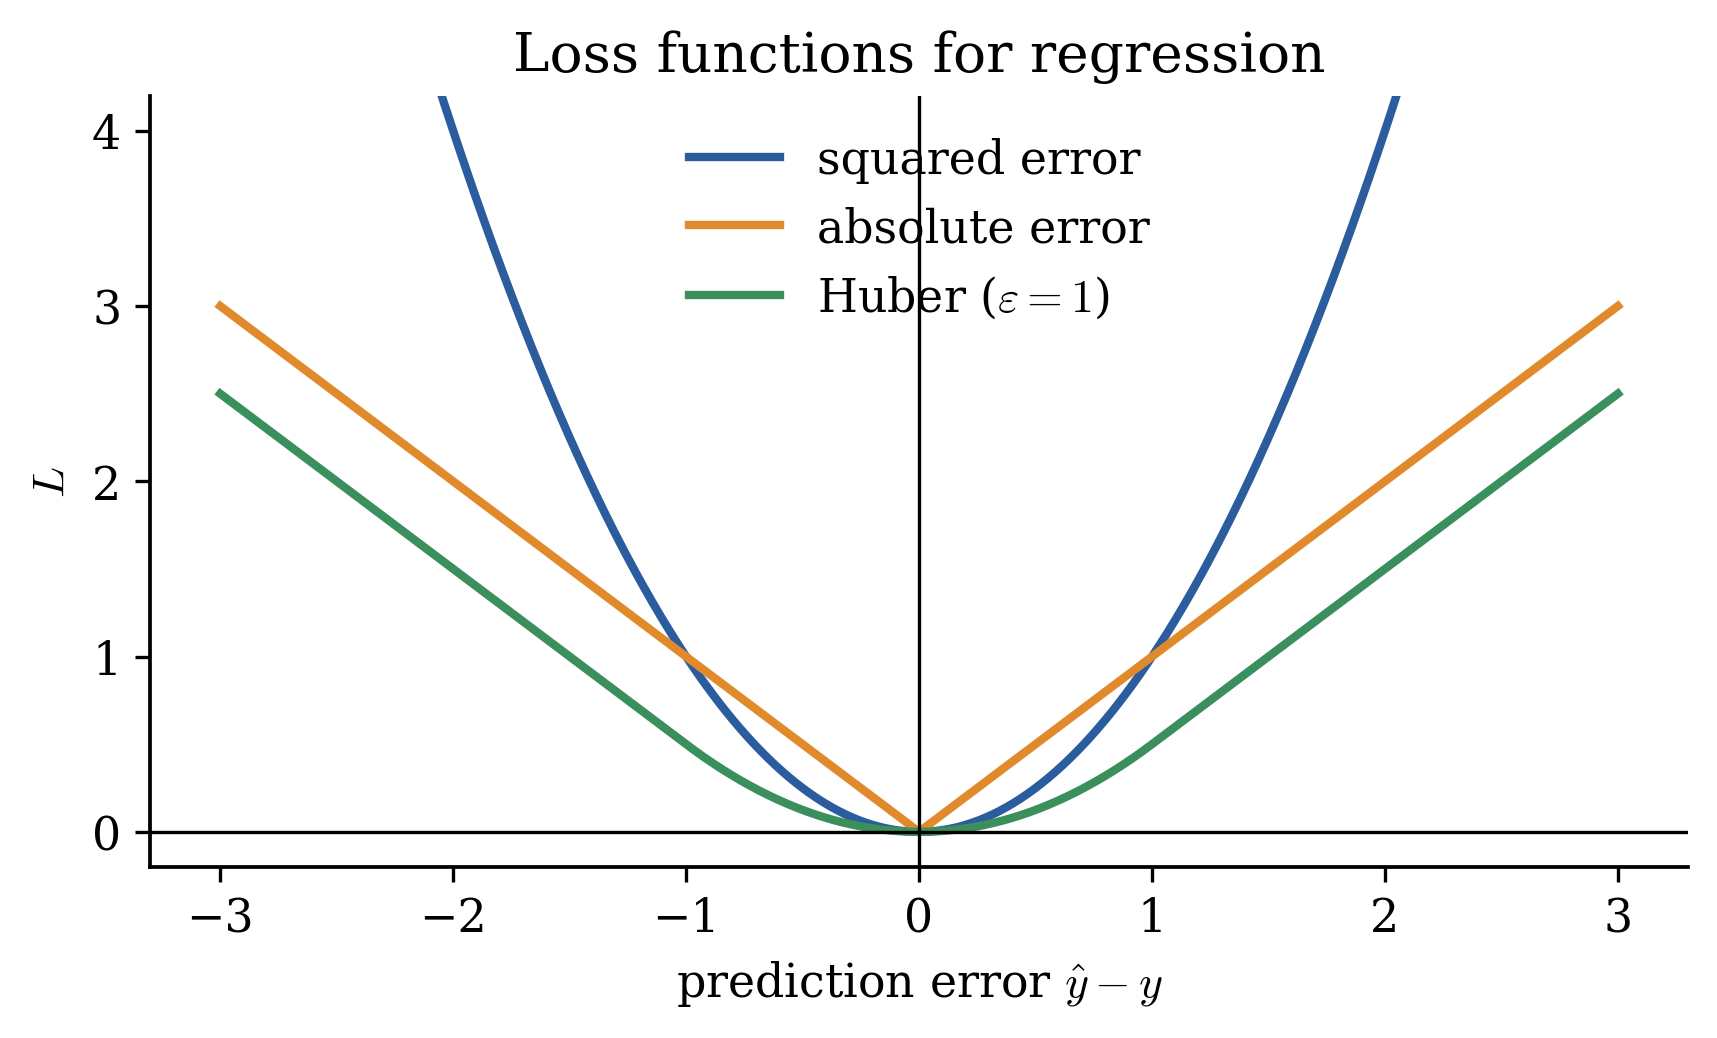
\includegraphics[width=0.65\textwidth]{images/chapter_6/sub_losses_regression.png}
    \caption{Loss functions for regression}
\end{figure}

\subsection{Squared Error Loss}
The squared error loss is defined as:
\[
L := (\widehat{y} - y)^2
\]

\begin{figure}[h]
    \centering
    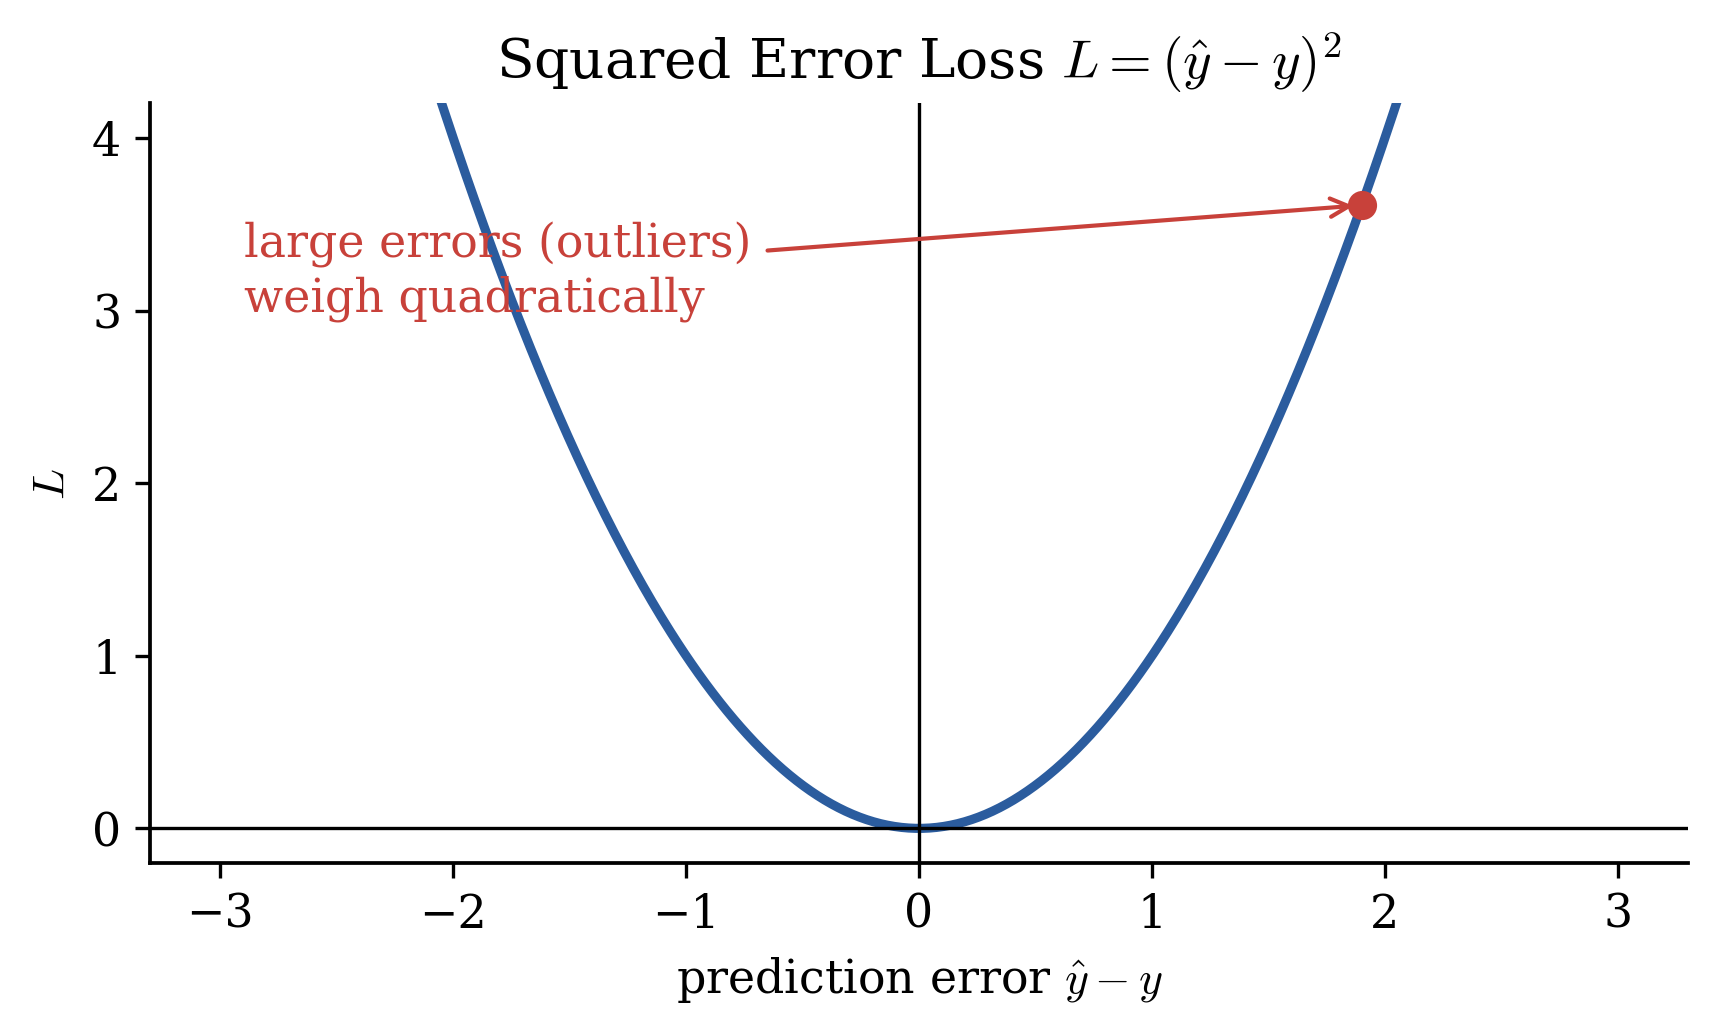
\includegraphics[width=0.65\textwidth]{images/chapter_6/sub_squared_loss.png}
    \caption{Squared Error Loss}
\end{figure}

Squaring makes large errors weigh much more than small ones: an error of 10 costs 100, while an error of 1 costs only 1. As a consequence, a single outlier can dominate the empirical risk and \textbf{pull the predictor towards itself}. On the other hand, the squared error is convex and differentiable, so it is easy to minimize. It is a good choice when the data contain \textbf{no outliers}.

\subsection{Absolute Error Loss}

The absolute error loss is defined as:
\[
L := |\widehat{y} - y|
\]

\begin{figure}[h]
    \centering
    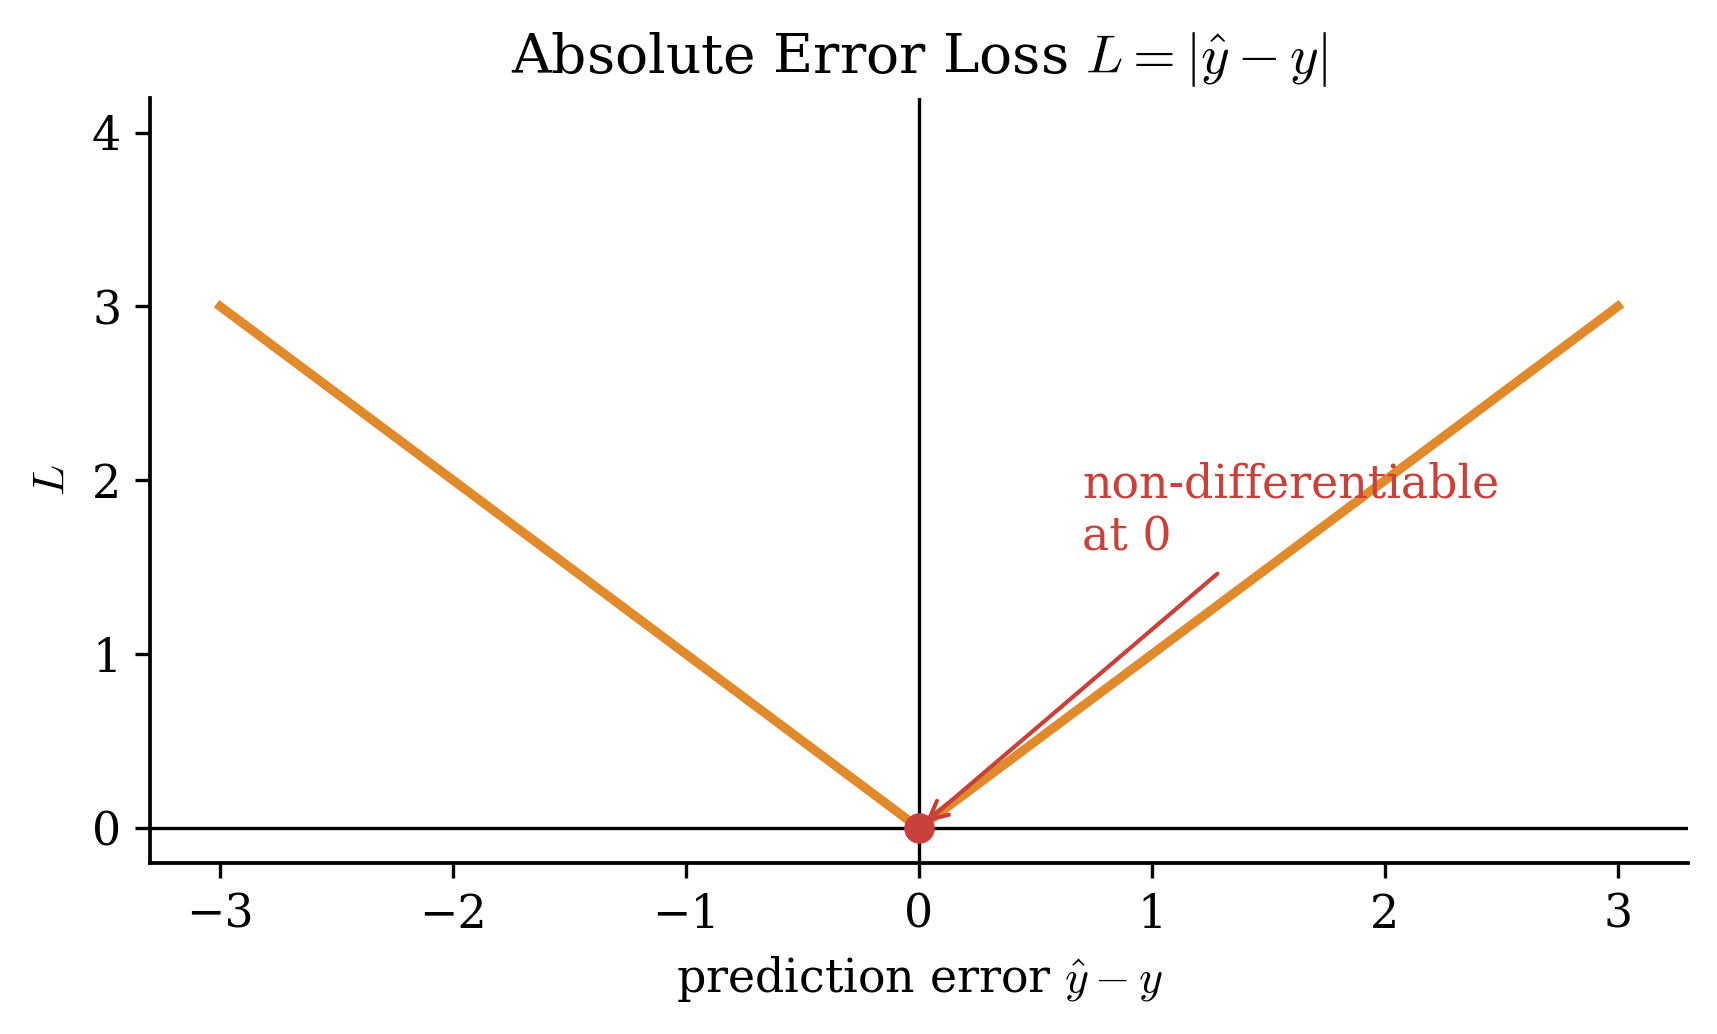
\includegraphics[width=0.65\textwidth]{images/chapter_6/sub_absolute_loss.png}
    \caption{Absolute Error Loss}
\end{figure}

Here the loss grows only \textbf{linearly} with the error, so an outlier counts in proportion to its distance and cannot dominate the others: the absolute error is \textbf{robust to outliers}. Its drawback is the corner at zero error, where the function is \textbf{not differentiable}. At that point the gradient is not defined, so gradient-based methods do not know in which direction to move.

\subsection{Huber Loss}
The Huber loss is defined as:
\[
L\big((\mathbf{x},y),h\big) =
\begin{cases}
(1/2)(y - h(\mathbf{x}))^2 & \text{for } |y - h(\mathbf{x})| \leq \varepsilon \\
\varepsilon(|y - h(\mathbf{x})| - \varepsilon/2) & \text{else.}
\end{cases}
\]

\begin{figure}[h]
    \centering
    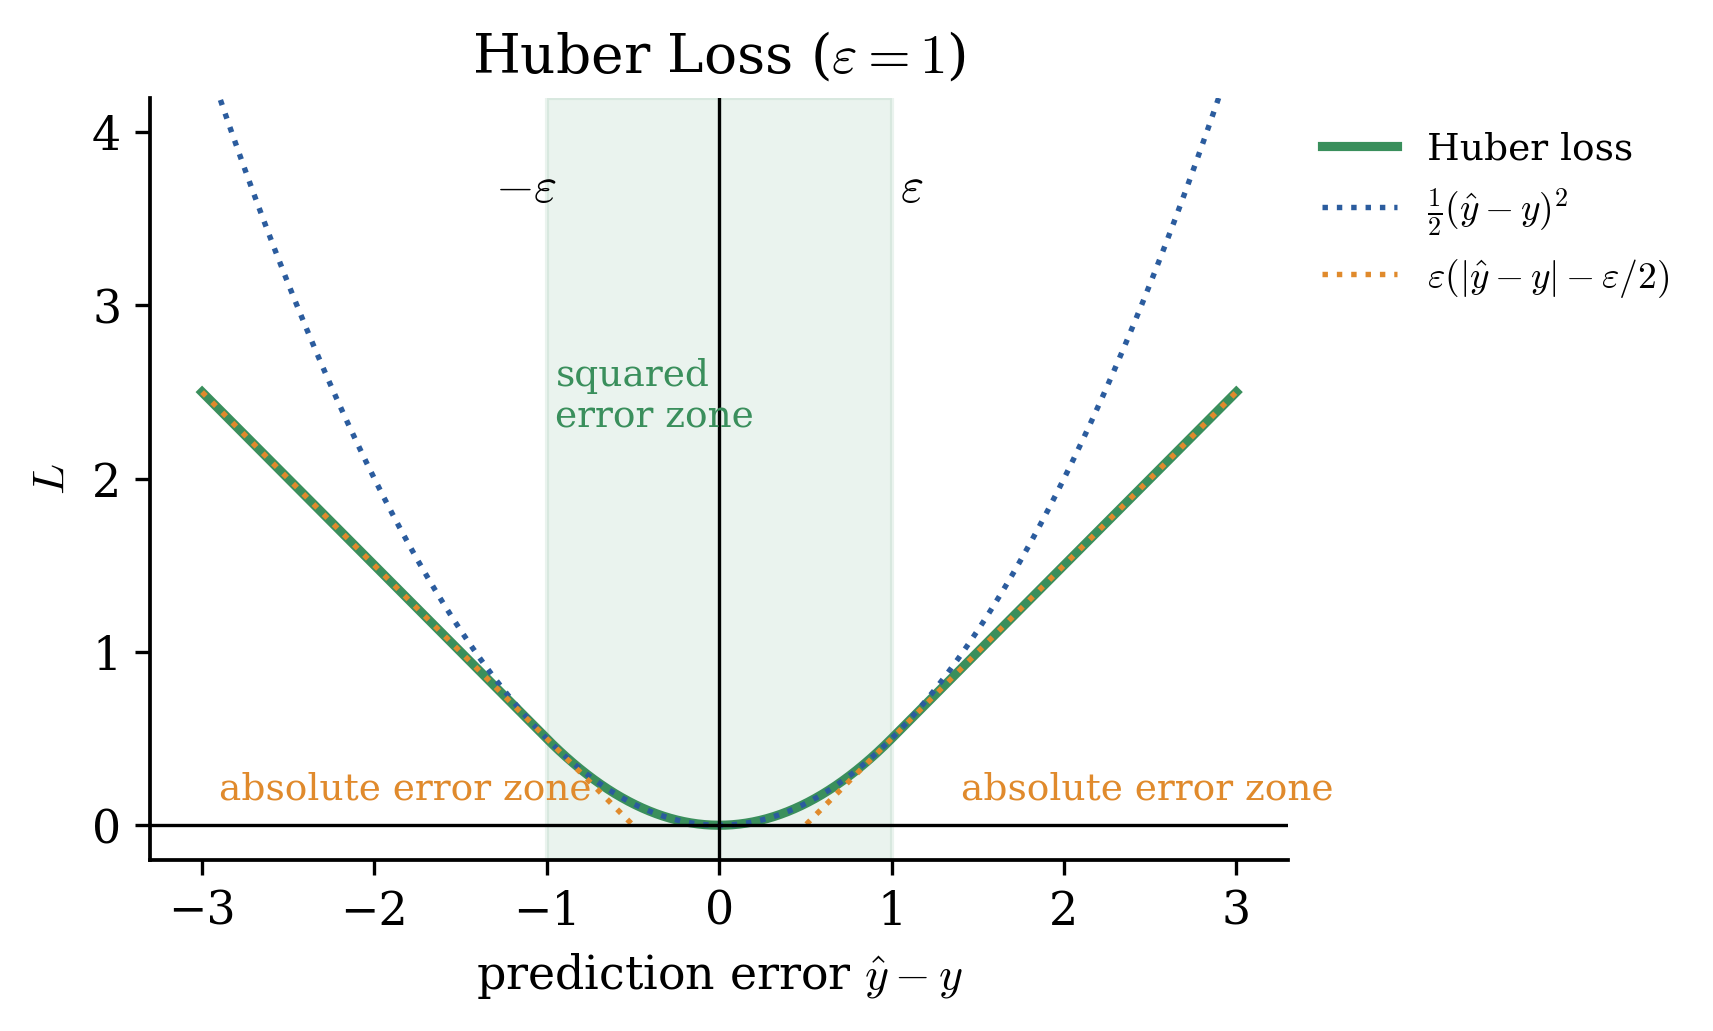
\includegraphics[width=0.8\textwidth]{images/chapter_6/sub_huber_loss.png}
    \caption{Huber Loss}
\end{figure}

The Huber loss combines the strengths of the previous two. For \textbf{small errors} (inside the $\varepsilon$ interval) it behaves like the squared error, so it is smooth and differentiable around zero. For \textbf{large errors} (outside the interval) it behaves like the absolute error, so outliers are tolerated. The constants $1/2$ and $\varepsilon/2$ make the two pieces join smoothly, so the function is differentiable everywhere.

To conclude, here is a comparison of the loss functions for regression:

\begin{center}
    \begin{tabular}{l|c|c|c}
        & \textbf{Robust to outliers} & \textbf{Insensitive to noise} & \textbf{Differentiable} \\ \hline
        Squared Error  & no  & yes & yes \\
        Absolute Error & yes & no  & no  \\
        Huber          & yes & yes & yes \\
    \end{tabular}
\end{center}

\textbf{Insensitive to noise} means that small deviations between the label $y$ and the prediction $h(\mathbf{x})$ have little effect on the loss. Squaring a small number makes it even smaller, which is why the squared error and the Huber loss have this property. All three losses are convex. Loss functions are preferred to be both \textbf{convex} and \textbf{differentiable}, since this makes them easier to minimize.


\section{ERM for Classification}
In classification the label is a \textbf{category}, for instance $y \in \{-1, +1\}$ in binary classification. Between categories there is no meaningful notion of distance, so the losses used for regression cannot be applied directly. The trick is to let the hypothesis still output a \textbf{real number} $h(\mathbf{x})$ and to read it in two parts:

\begin{itemize}
    \item its \textbf{sign} gives the predicted class: positive means $+1$, negative means $-1$;
    \item its \textbf{absolute value} $|h(\mathbf{x})|$ measures the \textbf{confidence} of the prediction: the farther from zero, the more sure the classifier is.
\end{itemize}
A classification loss is then built from this confidence: it should be small when the prediction is correct and confident, and large when it is wrong and confident.

\begin{figure}[h]
    \centering
    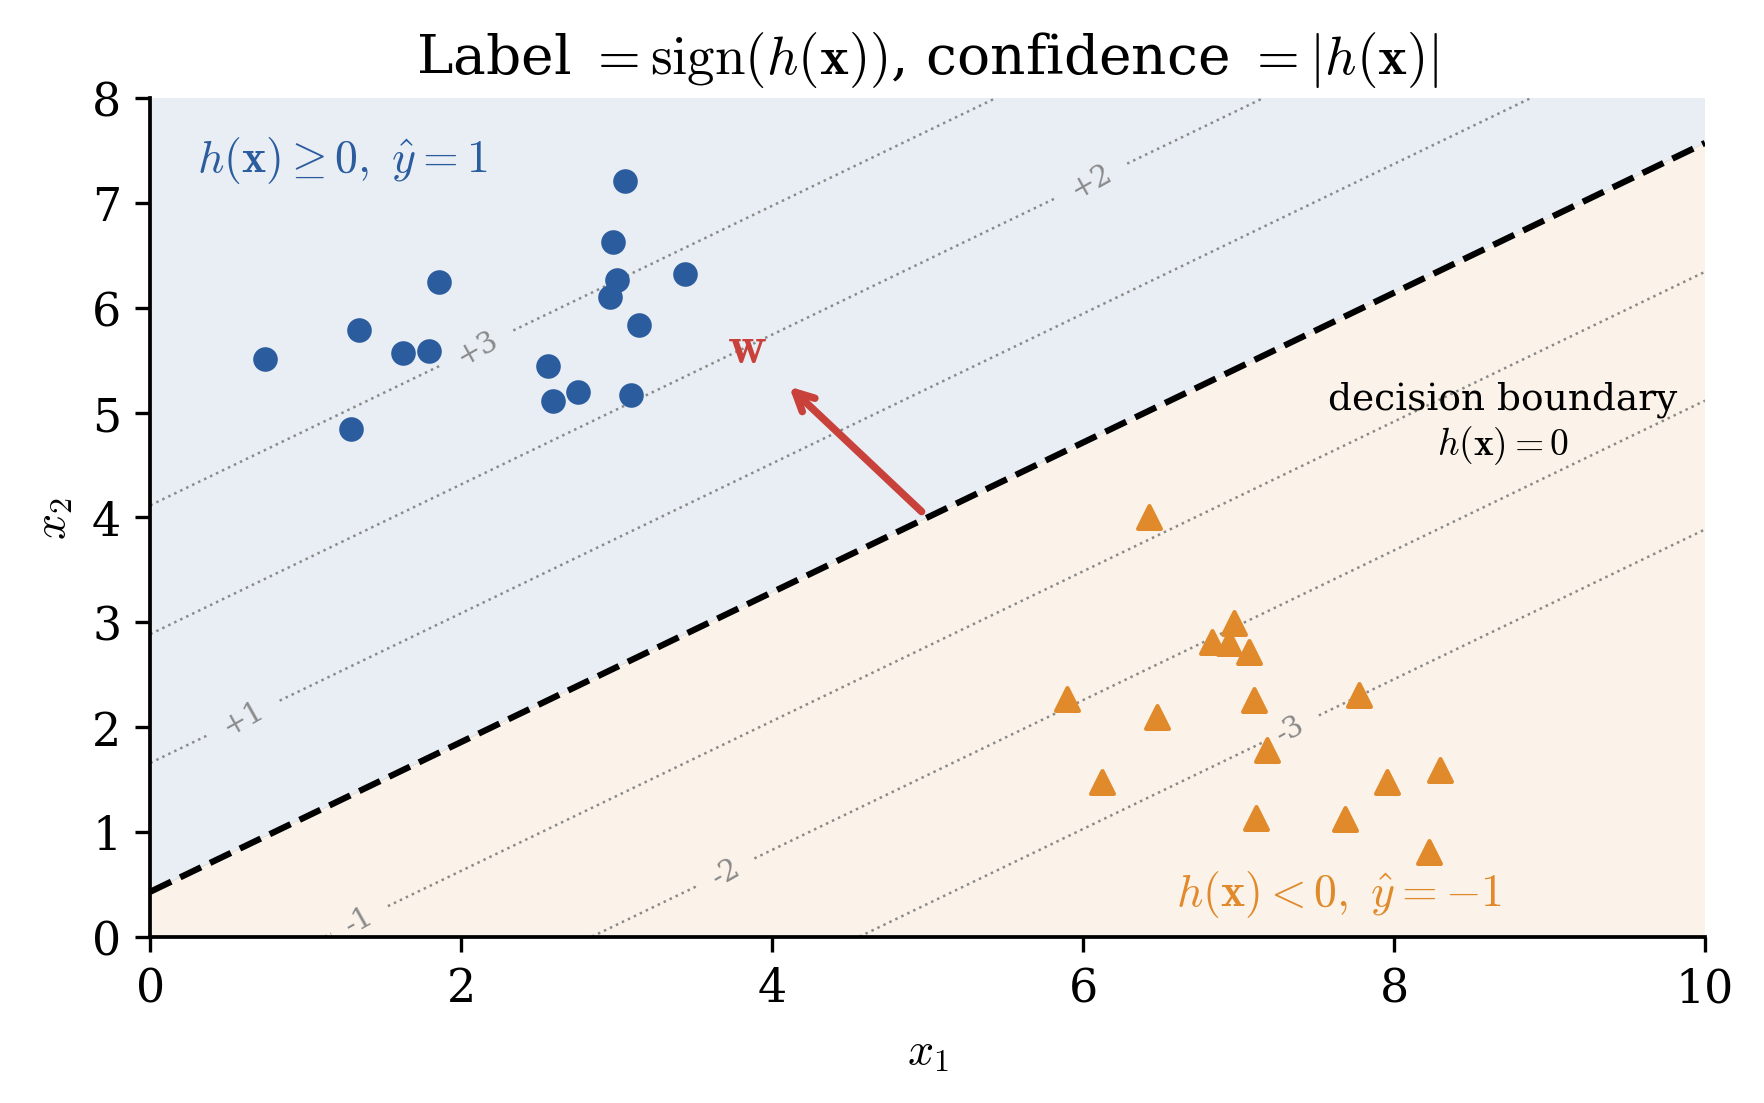
\includegraphics[width=0.7\textwidth]{images/chapter_6/sec_erm_classification.png}
    \caption{Linear classifier: label prediction and confidence}
\end{figure}

\subsection{Logistic Regression}
\textbf{Logistic Regression} is a binary classification method, and it is a clear example of the ERM recipe. It uses the same \textbf{data} (numeric features) and the same \textbf{model} (linear maps) as linear regression; the only thing that changes is the \textbf{loss}, which is the \textbf{logistic loss}:

\[
L\big((\mathbf{x},y),h\big) := \log\big(1 + \exp(-y h(\mathbf{x}))\big).
\]
The loss only depends on the product $y\,h(\mathbf{x})$. This product is positive when the predicted sign matches the true label (correct prediction) and negative otherwise. As a result:
\begin{itemize}
    \item correct and confident prediction ($y\,h(\mathbf{x})$ large and positive): the loss is close to zero;
    \item wrong prediction ($y\,h(\mathbf{x})$ negative): the loss grows, and it grows more the more confident the mistake is.
\end{itemize}

\begin{figure}[h]
    \centering
    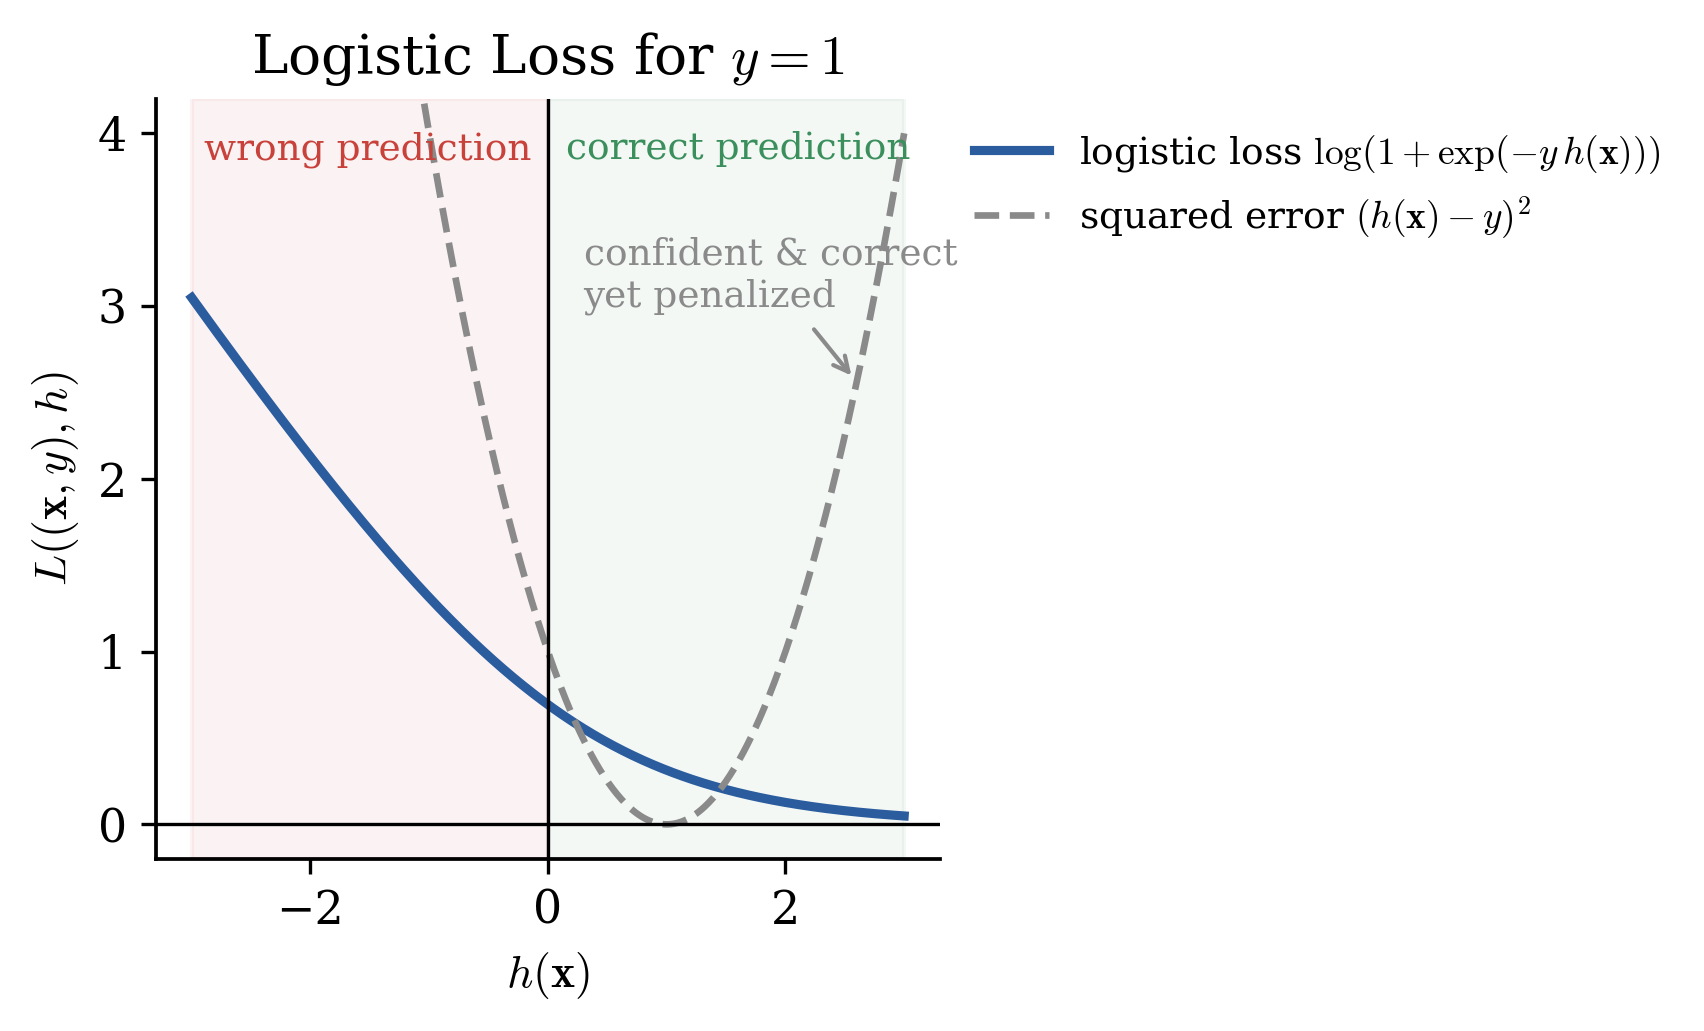
\includegraphics[width=0.85\textwidth]{images/chapter_6/sub_logistic_regression.png}
    \caption{Logistic Loss vs Squared Error Loss in classification}
\end{figure}

The logistic loss is \textbf{convex} and \textbf{differentiable}, so it is easy to minimize. The squared error loss, instead, is not suitable for classification. For example, if $y = 1$ and $h(\mathbf{x}) = 5$, the prediction is correct and very confident, yet the squared error is $(1-5)^2 = 16$. It \textbf{punishes the model for being confident and right}.

The \textbf{decision boundary}, i.e. the set of points where the classifier switches from one class to the other, is given by $h(\mathbf{x}) = 0$. Since $h$ is linear, this boundary is a straight line for two features (and a hyperplane in general).

\subsection{Loss Functions in Classification}
Besides the logistic loss, two other losses are common in classification:

\begin{itemize}
    \item \textbf{0/1 Loss}: it is $0$ if the prediction is correct and $1$ otherwise, so the empirical risk is simply the fraction of misclassified points. It measures exactly what we care about, but it ignores confidence and it is flat almost everywhere: it is \textbf{non-convex} and \textbf{non-differentiable}, and its gradient gives no direction to follow. For this reason it is used to \emph{evaluate} a classifier, not to train it.
    \item \textbf{Hinge Loss}: defined as $\max\big(0,\, 1 - y\,h(\mathbf{x})\big)$. It is zero when the prediction is correct with enough confidence ($y\,h(\mathbf{x}) \geq 1$) and grows linearly otherwise, so it also penalizes correct predictions that are not confident enough. It is \textbf{convex} but \textbf{not differentiable} at $y\,h(\mathbf{x}) = 1$. It is the loss used by Support Vector Machines.
\end{itemize}

\begin{figure}[h]
    \centering
    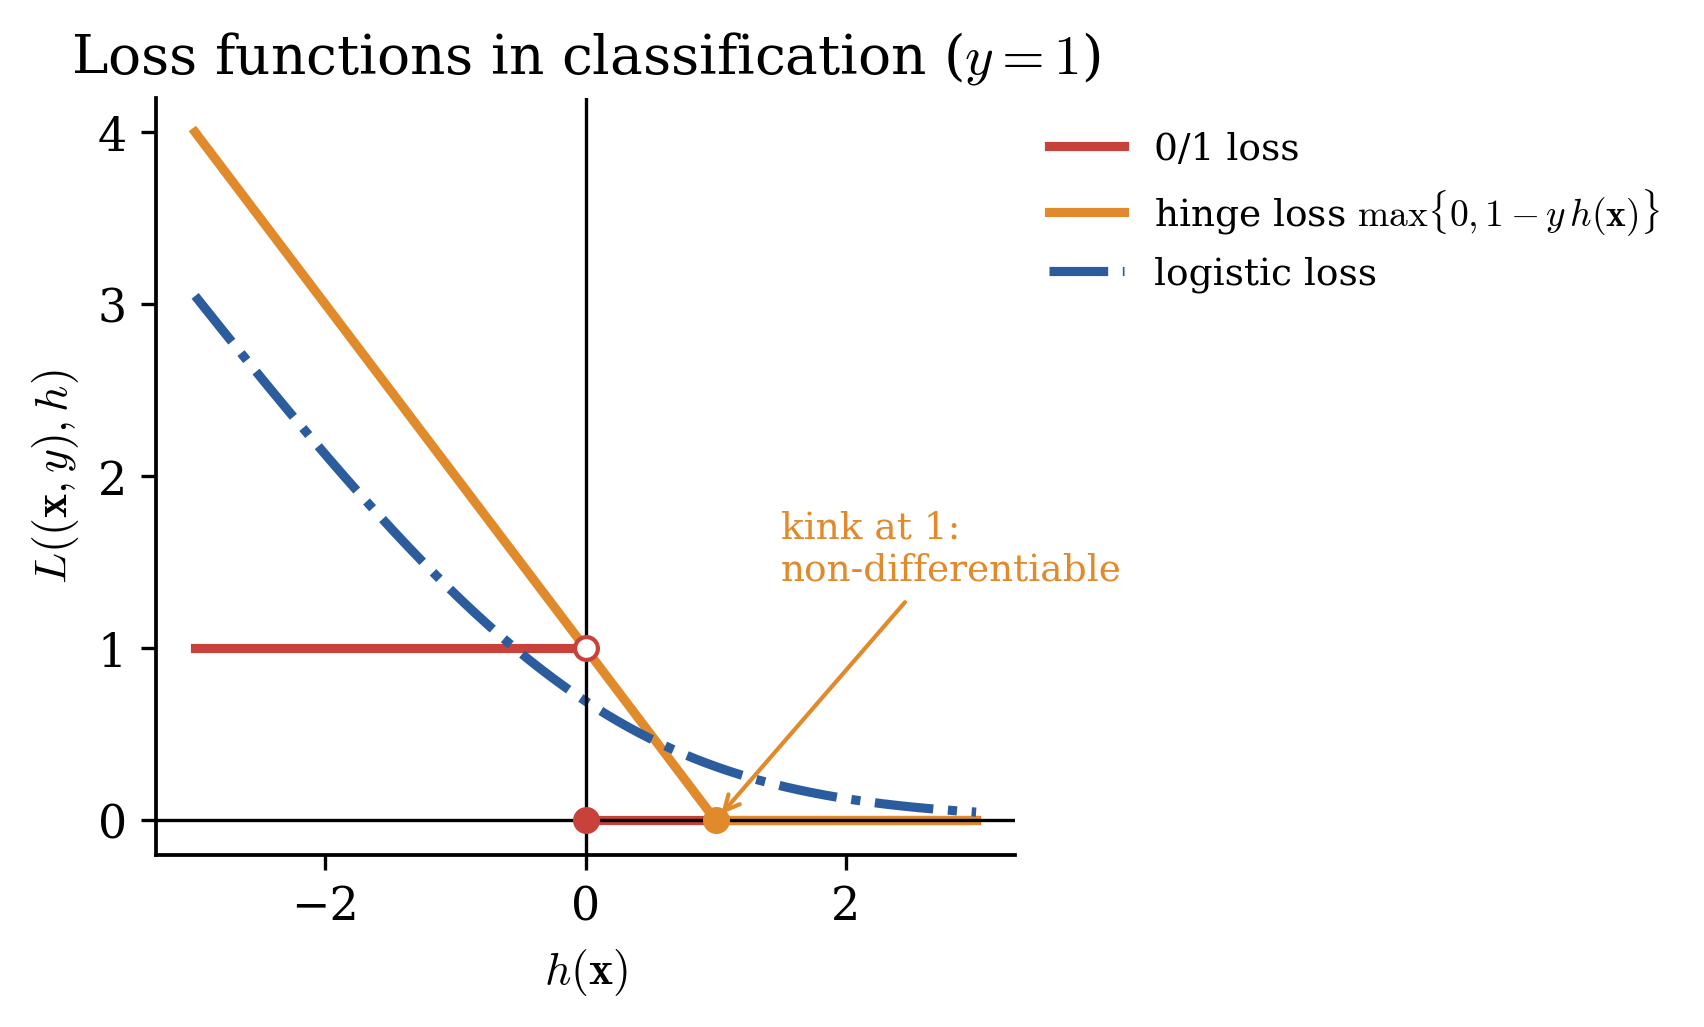
\includegraphics[width=0.6\textwidth]{images/chapter_6/sub_losses_classification.png}
    \caption{Loss functions in classification}
\end{figure}

\begin{center}
    \begin{tabular}{l|c|c|c}
        & \textbf{Uses confidence} & \textbf{Convex} & \textbf{Differentiable} \\ \hline
        0/1 Loss      & no  & no  & no  \\
        Hinge Loss    & yes & yes & no  \\
        Logistic Loss & yes & yes & yes \\
    \end{tabular}
\end{center}


\section{Summary}
\begin{figure}[h]
    \centering
    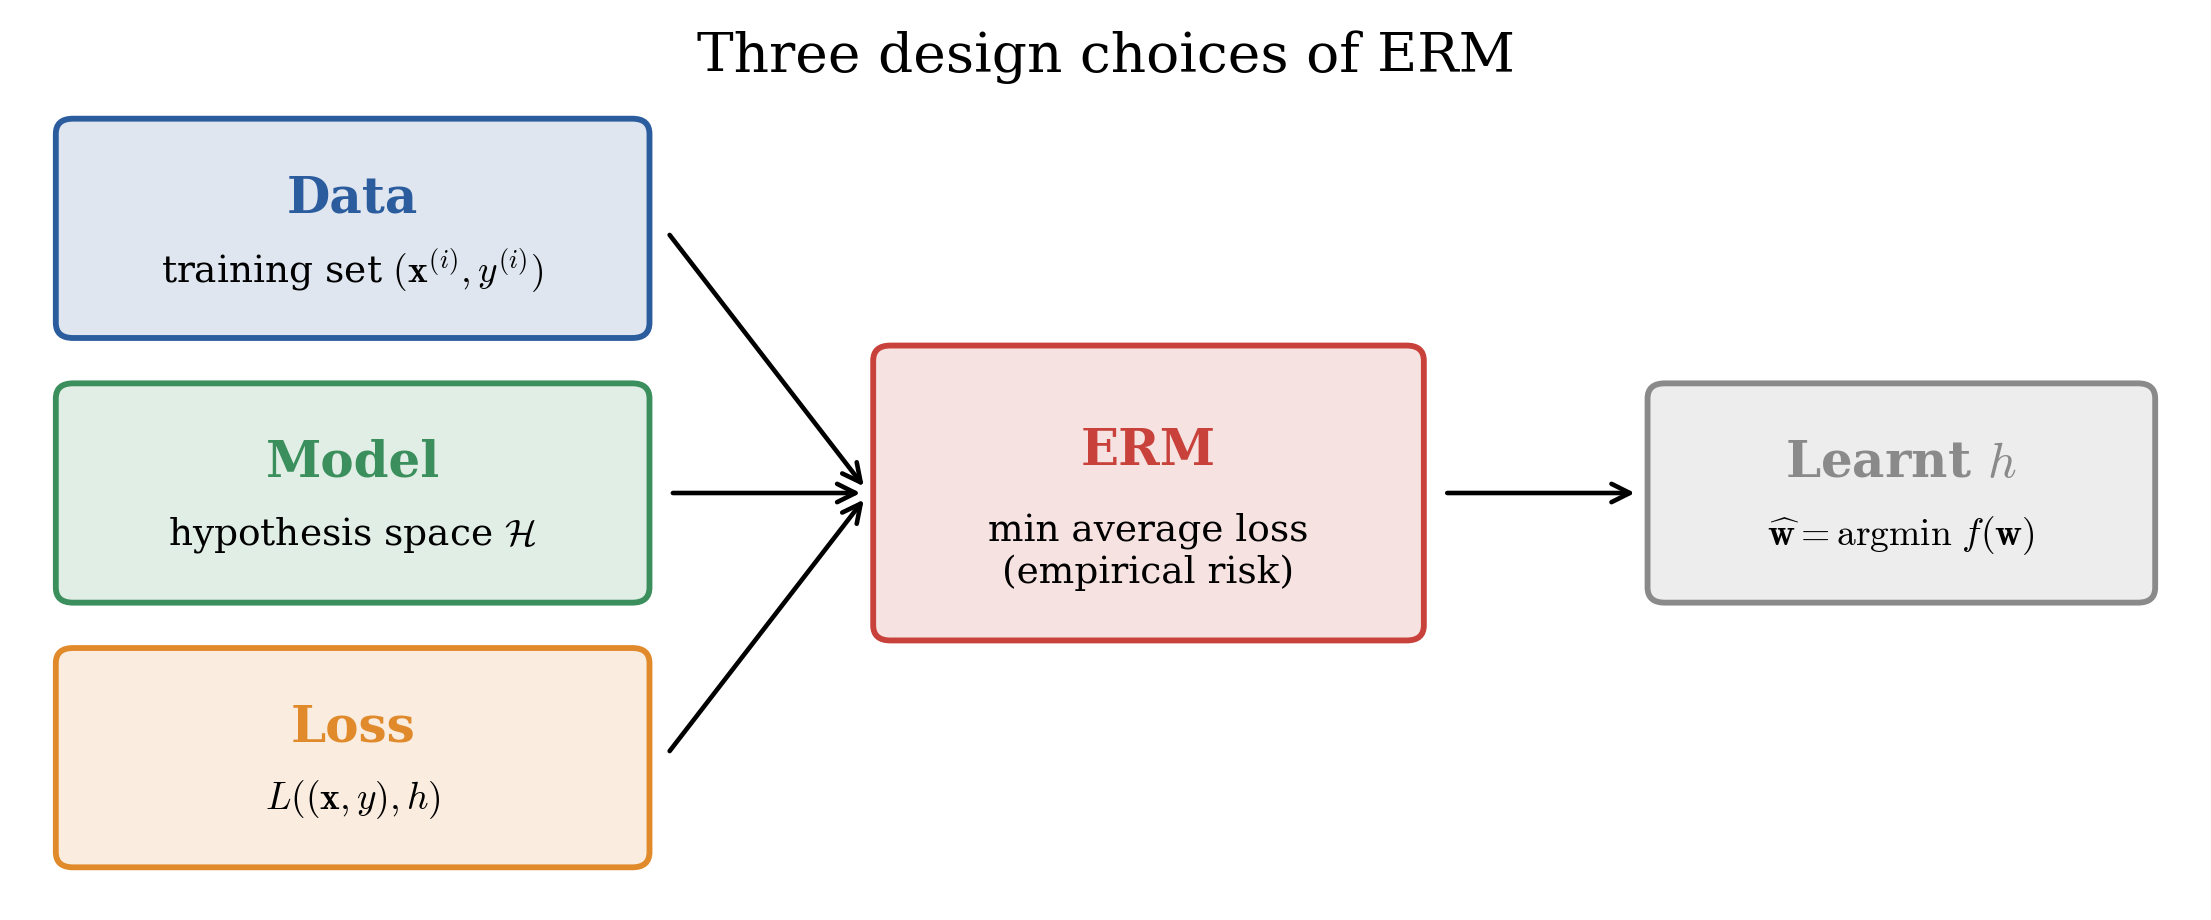
\includegraphics[width=0.5\textwidth]{images/chapter_6/sec_summary.png}
    \caption{Three design choices of ERM}
\end{figure}

\begin{itemize}
    \item The expected risk cannot be computed, so it is approximated by the \textbf{empirical risk}, the average loss on the training data.
    \item \textbf{ERM} learns the hypothesis with the smallest empirical risk. It can fail when the empirical risk is far from the expected risk.
    \item ERM is a general recipe based on \textbf{three design choices}: data, model and loss. Many ML methods are instances of ERM.
    \item Linear regression, polynomial regression and logistic regression are examples of ERM that differ only in some of these choices.
    \item In regression the loss measures a \textbf{distance} between numbers; in classification it is built from the \textbf{confidence} of the prediction.
    \item Convex and differentiable losses are preferred, since they are easier to minimize.
\end{itemize}





\section{A prova di coglione}

\subsection*{Il problema di fondo: non conosciamo la realtà}
Quello che vorremmo davvero è un'ipotesi $h$ che sbagli il meno possibile su \emph{qualsiasi} dato futuro, cioè che minimizzi il \textbf{rischio atteso}. Ma per calcolarlo servirebbe la distribuzione $p(x,y)$ da cui nascono i dati, e questa non la conosciamo mai. L'unica cosa che abbiamo è un campione: il training set.

L'idea centrale del capitolo è quindi una sostituzione: \textbf{al posto del rischio atteso usiamo la media delle loss sul training set}, il \textbf{rischio empirico}. Se i dati sono i.i.d. e abbastanza numerosi, la media sul campione è una buona stima della media sulla realtà. L'ERM consiste nello scegliere l'ipotesi che rende minima questa stima.

\begin{center}
    \fbox{\parbox{0.85\textwidth}{\centering
    \textbf{ERM è una scommessa:} che ciò che funziona bene sui dati di training funzioni bene anche sui dati che non abbiamo visto. Quando il rischio empirico si allontana da quello reale (pochi dati, dati non rappresentativi, modello troppo flessibile), la scommessa si perde.}}
\end{center}

\subsection*{ERM come ricetta: tre ingredienti}
L'ERM non è un singolo algoritmo ma uno \textbf{schema generale}. Per ottenere un metodo concreto bisogna fare tre scelte:
\begin{itemize}
    \item \textbf{Dati}: come rappresentiamo un punto (feature) e cosa vogliamo prevedere (label).
    \item \textbf{Modello}: lo spazio di ipotesi $\mathcal{H}$ tra cui cerchiamo, ad esempio tutte le funzioni lineari.
    \item \textbf{Loss}: come misuriamo quanto è grave un errore.
\end{itemize}

Cambiando anche uno solo degli ingredienti si ottiene un metodo diverso, ed è per questo che tanti metodi di ML sono in realtà casi particolari di ERM:

\begin{center}
    \begin{tabular}{l|l|l|l}
        & \textbf{Label} & \textbf{Modello} & \textbf{Loss} \\ \hline
        Linear Regression & numerica & mappe lineari & squared error \\
        Polynomial Regression & numerica & polinomi di grado $n$ & squared error \\
        Logistic Regression & binaria ($\pm 1$) & mappe lineari & logistic loss \\
    \end{tabular}
\end{center}

Notare che la Polynomial Regression non è un metodo nuovo: è la stessa regressione lineare applicata a feature trasformate ($x, x^2, \dots$). Si allarga il modello senza cambiare la ricetta.

Quando il modello è parametrizzato, cercare la migliore ipotesi equivale a cercare il miglior vettore di pesi: l'apprendimento diventa un \textbf{problema di ottimizzazione}, $\widehat{\mathbf{w}} = \operatorname{argmin}_{\mathbf{w}} f(\mathbf{w})$. Da qui l'importanza di loss \textbf{convesse} (un solo minimo, nessuna trappola) e \textbf{differenziabili} (il gradiente indica sempre la direzione in cui scendere).

\subsection*{La loss è dove decidiamo cosa conta}
La scelta della loss non è un dettaglio tecnico: \textbf{definisce che cosa significa ``sbagliare''}.

Nella \textbf{regressione} l'errore è una distanza tra numeri, e le tre loss viste sono tre atteggiamenti diversi verso gli errori grandi:
\begin{itemize}
    \item la \textbf{squared error} li punisce in modo quadratico, quindi è comoda da ottimizzare ma si lascia trascinare dagli outlier;
    \item la \textbf{absolute error} li tratta in proporzione, quindi è robusta agli outlier ma ha un punto angoloso in cui il gradiente non è definito;
    \item la \textbf{Huber loss} è il compromesso: quadratica per errori piccoli, lineare per quelli grandi. Prende il meglio delle altre due.
\end{itemize}

Nella \textbf{classificazione} la prospettiva cambia. Il modello produce comunque un numero $h(\mathbf{x})$, ma lo leggiamo in due parti: il \textbf{segno} dice la classe, il \textbf{modulo} dice quanto il modello ne è sicuro. Il confine tra le classi è dove $h(\mathbf{x}) = 0$, che per un modello lineare è una retta (o un iperpiano).

Una buona loss di classificazione deve quindi \textbf{premiare la sicurezza quando è giusta e punirla quando è sbagliata}. È esattamente qui che la squared error fallisce: penalizza un $h(\mathbf{x})$ molto grande anche quando la previsione è corretta, cioè punisce il modello per essere sicuro e nel giusto. La \textbf{logistic loss} invece decresce man mano che la previsione corretta diventa più sicura, ed è convessa e differenziabile. La \textbf{0/1 loss} conta semplicemente gli errori, ed è ciò che in fondo vogliamo misurare, ma è inutilizzabile come obiettivo da ottimizzare perché non è né convessa né differenziabile. La \textbf{hinge loss} è convessa ma ha un punto angoloso.

\subsection*{Il messaggio da portare a casa}
\begin{center}
    \fbox{\parbox{0.85\textwidth}{\centering
    Imparare significa \textbf{minimizzare l'errore medio sui dati che abbiamo}, sperando che rifletta l'errore sui dati che non abbiamo. Ogni metodo di ML nasce da tre scelte (dati, modello, loss), e la loss è quella che più di tutte decide sia \emph{cosa} il modello impara sia \emph{quanto facilmente} riusciamo a fargliela imparare.}}
\end{center}



\end{document}
% -----------------------------------------------------------------
